\documentclass[a4paper,11pt]{book}
\usepackage[dvipsnames]{xcolor}
%********************************************************
%**************** Chargement des paquets ****************
%********************************************************
%-------------------------------------%******************
%-------------------------------------%   MISE EN PAGE  *
%-------------------------------------%******************
\usepackage[a4paper, left=2.5cm, width=16cm, height=25.4cm, includehead, includefoot, headheight=13.6pt]{geometry}
\usepackage{multicol}                 % Ecrire en colones \begin{multicols}{2} \end{multicols}
\usepackage[explicit]{titlesec}	  	  % Titres personalisables
\usepackage{titletoc}                 % Table des matières
\usepackage[hidelinks]{hyperref}      % Lien vers les chapitres en table de matières
\usepackage{fancyhdr}		          % En-tête et pied de page
\usepackage{enumitem}                 % Enumérations
\usepackage{fancyvrb}                 % Augmente les possibilités de verbatim
%-------------------------------------%******************
%-------------------------------------%    CARACTERES   * 
%-------------------------------------%******************
\usepackage[utf8]{inputenc}           % Encodage du fichier source en utf8
\usepackage[T1]{fontenc}	          % Encodage du fichier de sortie
\usepackage{lmodern}				  % Police vectoriel
\usepackage[francais]{babel}          % Conventions typographiques
\usepackage{eurosym}                  % Le symbole € par \euro{}
%-------------------------------------%******************
%-------------------------------------%  MATHEMATIQUES  *
%-------------------------------------%******************
\usepackage{amsmath,                  % Mise en forme de formules, équations
            amsfonts,                 % Symboles, tailles adaptées, Fraktur, Cyrillic
            amssymb,                  % Symboles mathématiques (e.g. \mathbb{R} )
            amsthm}                   % Personalisation des théorèmes
\usepackage{mathrsfs}                 % Pour l'écriture cursive \mathscr{C}
\usepackage[np]{numprint}	          % Pour l'écriture des nombres \np{3250.58}
%-------------------------------------%******************
%-------------------------------------%     TABLEAUX    *
%-------------------------------------%******************
\usepackage{array,                    % Tableaux plus riches que tabular simple
            multirow,                 % Pour fusionner des lignes
            makecell}	              % Autres macro de manipulation des lignes
\usepackage{colortbl}	              % Couleurs de fond
%-------------------------------------%******************
%-------------------------------------%    GRAPHIQUES   *
%-------------------------------------%******************
\usepackage{color}
%-------------- TIKZ -----------------
\usepackage{pgf,tikz}			 	  % Dessinner avec tikz
\usetikzlibrary{shapes,               % d'autres formes
           decorations.pathreplacing, % pour les accolades
           calc,                      % Calculs de coordonnées entre $ $
           patterns,                  % Pour les remplissages
           intersections,             % Calcul d'intersections de chemins
           automata,
           positioning,
           graphs,
           matrix,
           shadows.blur,
           shadings,
           shapes.callouts,
           shapes.arrows,
           angles}
\pgfdeclarelayer{background}
\pgfsetlayers{background,main}
\usepackage[tikz]{bclogo}             % Les boites avec logo ( dans \Cours )
\usepackage{graphicx}	              % Inclusion d'images
\usepackage[oldvoltagedirection]{circuitikz} % Pour les portes logiques

%********************************************************
%************ PERSONALISATIONS ET RACOURCIS *************
%********************************************************
\usepackage{xifthen}                  % pour les tests \isempty des commandes
%------------------ Table des matières ------------------
%--------------------------------------------------------
\renewcommand{\thepart}{\Alph{part} }
\renewcommand{\chaptermark}[1]{\markboth{\bsc{#1}}{}}
\makeatletter\@addtoreset{chapter}{part}\makeatother
\titlecontents{part}[0em]             % Titre de partie, centrée
  {\bigskip\bfseries\large\centering} % Grand espacé, gras, grand, centrée
  {}
  {}
  {}
\titlecontents{chapter}[2em]          % Titre de chapitre
  {\contentsmargin{10mm}\medskip\bfseries}                 % Espacé, gras
  {\contentslabel{1.5em}}             % Réservation de l'espace du n°
  {}
  {\hfill\contentspage}               % Avec le n° de page
\titlecontents{section}[3.5em]        % Titre de section
  {\smallskip}                        % Petit espacé
  {\contentslabel{1.5em}}             % Réservation de l'espace du n°
  {}
  {\titlerule*[0.75em]{.}\contentspage}% N° de page au bout de pointillés
%--------------------------------------------------------
%---- Commande \partie{...} à substituer à \part{...} ---
\newcommand{\partie}[2][]{
  % Le paramètre optionnel est un titre court -----------
  \ifthenelse{\isempty{#1}}{\def\nom{#2}}{\def\nom{#1}}
  % Définition des en-têtes -----------------------------
  \pagestyle{fancy}
  \lhead[\bsc{#2 (\thechapter\!)}]{}  % Nom de la partie en petite maj. page de gauche
  \chead{}                            % Centre du pied de l'entête vide
  \rhead[]{\leftmark}                 % Nom du Chapitre en petite maj. page de droite
  \renewcommand{\headrulewidth}{0.5pt}% souligné d'une barre de 0.5pt
  \lfoot[\thepage]{}                  % numéro de page, page de gauche à gauche
  \cfoot{}                            % Centre du pied de page vide
  \rfoot[]{\thepage}                  % numéro de page, page de droite à droite
  % Formatage des titres de chapitre -------------------
  % Ici pour ne pas être effectif pour la table des matières et l'avant propos.
  \renewcommand{\thechapter}{\Roman{chapter} }
  \titleformat{\chapter}[display] 
    {\LARGE \bfseries}
    {\mbox{\nom (\thechapter\!)}\\
    \vspace{-1em}\hrule\vspace{-1ex}
    \flushright\mbox{##1}}
    {0pt}
    {\tiny}[]
  \titlespacing*{\chapter}{0cm}{-1.5cm}{-0.2cm}[0pt]
  % Début de la partie ---------------------------------
  \part*{#2}                           % Sans numérotation visible
  \stepcounter{part}                   % Mais tout de même numéroté
  \setcounter{chapter}{0}              % Avec réinitialisation des n° de chapitre
  \addcontentsline{toc}{part}{#2}      % Et affichage en table des matières
  \newpage\ifodd\thepage\else\thispagestyle{empty}\fi
}
%--------------------------------------------------------
%--------------- Formatage des sections -----------------
\renewcommand{\thesection}{\arabic{section}}
\titleformat{\section}  
  {\gdef\sectionlabel{}\Large\bfseries}
  {\gdef\sectionlabel{\thesection }}{0pt}
  {\begin{tikzpicture}[remember picture, overlay]
       \node[anchor=west,xshift=-1,rectangle,draw,line width=0.5pt,
              rounded corners=2pt,inner sep=4pt]
              {\color{black}\sectionlabel~-~#1};
       \end{tikzpicture}}
\titlespacing*{\section}{2pt}{\baselineskip}{\baselineskip}
%--------------------------------------------------------
%------------ Formatage des sous-sections ---------------
\renewcommand{\thesubsection}{\alph{subsection})~}
\titleformat{\subsection}  
  {\large\bfseries}
  {\thesubsection}{0pt}
  {#1}
\titlespacing*{\subsection}{2pt}{1em}{0.5em}
%--------------------------------------------------------
%--------------- Formatage des listes -------------------
\setlist[itemize,1]{label=$\star$}     % Remplace la pastille de niveau 1 par une étoile
%--------------------------------------------------------
%------- espacement verticaux d'un multicols ------------
\multicolsep\itemsep                   % Comme pour les listes
%********************************************************
%-------------- La commande \Cours{...} -----------------
%--------------------------------------------------------
\renewcommand\bcStyleTitre[1]{\hspace{0.6cm}\bfseries#1}
\newcommand\bccours{
\includegraphics[width=\logowidth]{loupe}}
\newcommand{\Cours}[1]{
  \begin{bclogo}[logo=\bccours, noborder, epBarre=1, couleurBarre=black,marge=0]
    {}\vspace{-.5cm}\hspace{\parindent}#1
  \end{bclogo}
}
%-------------- La commande \date{...} ------------------
%--------------------------------------------------------
\renewcommand\date[1]{\begin{tikzpicture}[baseline = (A.base)]
\node(A)[draw,line width=0.5pt, rounded corners=2pt,inner sep=2pt,single arrow]{\color{black}#1};
\end{tikzpicture}}
%********************************************************
%----------------------- Tableaux -----------------------
%--------------------------------------------------------
%------- Pour spécifier la largeur d'une case -----------
\newcolumntype{R}[1]{>{\raggedleft\arraybackslash }m{#1}}
\newcolumntype{L}[1]{>{\raggedright\arraybackslash }m{#1}}
\newcolumntype{C}[1]{>{\centering\arraybackslash }m{#1}}
\newcolumntype{T}[1]{>{\raggedright\arraybackslash }p{#1}}
%********************************************************
%----------------------- Couleurs -----------------------
%--------------------------------------------------------
\definecolor{rouge}{RGB}{155,0,0}
\definecolor{vert}{RGB}{0,176,80}
\definecolor{bleu}{RGB}{0,112,192}
\definecolor{jaune}{RGB}{255,255,0}
\definecolor{bo}{RGB}{23,129,142}

%\newlength{\currentparindent}%

%********************************************************
%--------------------- Informatique ---------------------
%--------------------------------------------------------
%--------------------- Python ---------------------
\usepackage{minted} %[cache=true]
\setminted{python3=true,fontsize=\small,frame=leftline,numbers=left,numbersep=2pt,resetmargins=true,xleftmargin=1em, style = xcode,bgcolor=black!5}
%liste des styles : pygmentize -L styles
\newmintinline{python}{python3, fontsize=\small, style = xcode,bgcolor=black!5}
\newmintinline{asm}{fontsize=\small, style = xcode,bgcolor=black!5}

%--------------------- Algorithmes ---------------------
\usepackage[french,boxed,vlined,longend,linesnumbered]{algorithm2e} 
% lined peut être 
% ----- vlined ce qui fait dispaitre les << fin ... >>
% ----- noline pour ne pas tracer les lignes des blocs
% longend peut être shortend (par défaut) ou noend
\DontPrintSemicolon                            % n'affiche pas les << ; >> de fin d'instruction
\SetKw{Retour}{renvoyer}                       % Redéfinition possible de tous les mots clefs
\SetKwProg{Fct}{fonction}{}{fin fonction}      % Définition possible d'autres environnements

%--------------------- Shell ---------------------
\newcommand{\cmd}[1]{\tikz[baseline=(C.base)]\node[fill=black, inner sep =0pt](C){\strut\texttt{\color{white}\bfseries #1}};}
\newsavebox{\FVerbBox}
\newenvironment{shell}{\VerbatimEnvironment%
\begin{lrbox}{\FVerbBox}%
\begin{minipage}{\linewidth-2\fboxsep-\parindent}%-2\fboxrule
\color{white}%
\begin{Verbatim}}%
{\end{Verbatim}%
\end{minipage}%
\end{lrbox}%
\colorbox{black}{\usebox{\FVerbBox}}}%\fcolorbox{black}{black!10}{\usebox{\FVerbBox}}}


\begin{document}

%---------------------- logos ---------------------


\def\serveur{\begin{tikzpicture}[scale=0.25]
\draw[rounded corners=1pt, fill=white](-2.5,-2)rectangle(1,4);
\draw(0.5,3.5)circle(0.3);
\foreach \y in {0,-1.2,-2.4} {
\draw[yshift=\y cm](-2,2)rectangle(0.5,3);
\draw[yshift=\y cm](-1.7,2.7)--(-1.7,2.3)-|(0.2,2.7);}
\foreach \y in {-0.5,-0.1,0.3}
\fill[black!15,yshift=\y cm](-2,-1)rectangle(0.5,-1.2);
\end{tikzpicture}}

\def\imprimante{\begin{tikzpicture}[scale=0.2]
\draw[rounded corners=2pt,fill=black!15](0,0)rectangle(4,2);
\draw[fill=white](3.5,1.5)circle(0.3);
\draw[fill=white](0.5,0.75)rectangle(3.5,-0.5);
\draw[fill=white](0.5,2)rectangle(3.5,3.5);
\foreach \y in {0,-0.25,...,-0.75}
\fill[yshift=\y cm](0.75,0.5)rectangle(3.25,0.55);
\end{tikzpicture}}

\def\telephone{\begin{tikzpicture}[scale=0.1]
\draw[rounded corners=2pt,fill=white](-0.5,-0.8)rectangle(2.5,4.5);
\draw[rounded corners=1pt,fill=black](0,0)rectangle(2,4);
\draw(1,-0.4)circle(0.2);
\end{tikzpicture}}

\def\ordinateur{\begin{tikzpicture}[scale=0.15]
\draw(3.5,-2)ellipse(2 and 0.25);
\draw[fill=white](3,-2)rectangle(4,0);
\draw[rounded corners=1pt, fill = white](-2.5,-2)rectangle(1,4);
\draw(-0.75,3)circle(0.3);
\draw(-2,1.5)rectangle(0.5,2.5);
\foreach \y in {0,0.5,1}
\fill[black!15,yshift=\y cm](-2,-1)rectangle(0.5,-1.2);
\draw[rounded corners=2pt,fill=white](-0.5,-0.8)rectangle(7.5,4.5);
\draw[rounded corners=1pt,fill=black](0,0)rectangle(7,4);
\draw(3.5,-0.4)circle(0.2);
\end{tikzpicture}}

\def\routeur{\begin{tikzpicture}[xscale=0.12,yscale=0.06]
\def\fleche{(0,-0.5)-|(2,-1)--(3,0)--(2,1)|-(0,0.5)--cycle}
\draw[fill=black!15](0,-2)circle(4);
\draw[fill=black!15](-4,-2)--(-4,0)-|(4,-2);
\draw[fill=black!15](0,0)circle(4);
\draw[rotate=-30,xshift=-3.5cm,fill=white] \fleche;
\draw[rotate=150,xshift=-3.5cm,fill=white] \fleche;
\draw[rotate=60,xshift=0.5cm,fill=white] \fleche;
\draw[rotate=240,xshift=0.5cm,fill=white] \fleche;
\end{tikzpicture}}

\def\switch{\begin{tikzpicture}[xscale=0.07,yscale=0.06]
\def\fleche{(0,-0.5)--(4,-0.5)--(3.9,-1)--(5.5,0)--(4.3,1)--(4.2,0.5)--(0.2,0.5)--cycle}
\draw[fill=black!15](-7,-6)rectangle(5.6,-3);
\draw[fill=black!15](5.6,-3)--(5.6,-6)--(7,1)--(7,4)--cycle;
\draw[fill=black!15](-7,-3)--(-5.6,4)--(7,4)--(5.6,-3)--cycle;
\draw[fill=white] \fleche;
\draw[yshift=2.5cm,xshift=0.5cm,fill=white] \fleche;
\draw[yshift=1.25cm,fill=white,rotate=180] \fleche;
\draw[yshift=-1.25cm,xshift=-0.5cm,fill=white,rotate=180] \fleche;
\end{tikzpicture}}

\def\accesWiFi{\begin{tikzpicture}[scale=0.25]
\draw[color=black,fill=black!15,rounded corners=3pt](-2,0)rectangle(2,1);
\draw[color=white,fill=white,rounded corners=3pt](0,0.1)rectangle(1.9,0.9);
\draw[color=white,fill=white,rounded corners=3pt](-1,0.1)rectangle(1,0.5);
\draw[color=black!15,fill=black!15,rounded corners=3pt](0,0.1)rectangle(-1.9,0.9);
\draw[line width = 1pt](-1.8,-0.2)--(1.8,-0.2);
\draw[line width = 2pt](-1.6,1.2)--(-1.6,2.2);
\draw[line width = 1pt](-1.6,2.2)--(-1.6,3);
\draw[line width = 1pt](-1.6,3)++(45:0.33) arc (45:135:0.33);
\draw[line width = 1pt](-1.6,3)++(45:0.66) arc (45:135:0.66);
\draw[line width = 1pt](-1.6,3)++(45:1) arc (45:135:1);
\end{tikzpicture}}

%--------------------------------------------------------
%------ vide la page pour le titre et le sommaire -------
\pagestyle{empty}
\fancypagestyle{plain}{%
  \fancyhf{}
  \fancyfoot[C,L,R]{}
  \renewcommand{\headrulewidth}{0pt}
}

{\centering
\begin{tikzpicture}[line width=2pt,rounded corners=1pt,cap=round,scale=3]\huge
\draw[fill=black!5] (0,0)rectangle++(1,1)node[midway,scale=2]{N};
\draw[fill=black!5] (1.15,0)rectangle++(1,1)node[midway,scale=2]{S};
\draw[fill=black!5] (2.3,0)rectangle++(1,1)node[midway,scale=2]{I};
\draw[fill=black!5] (0,-1.15)rectangle++(1,1)node[midway,scale=0.66]{Numétique};
\draw[fill=black!5] (1.15,-1.15)rectangle++(1,1)node[midway,scale=0.66]{\& Sciences};
\draw[fill=black!5] (2.3,-1.15)rectangle++(1,1)node[midway,scale=0.6]{\texttt{Informatiques}};
\node[scale=1]at(1.65,1.5){Synthèse de cours 2019-2020 de};
\node[scale=1,inner sep = 2mm](S)at(1.65,-1.65){Spécilialité de première générale};
\draw[line width=1pt](S.north east)--(S.north west)(S.south east)--(S.south west);
\end{tikzpicture}\par}


\chapter*{Avant-propos}


\vspace{\stretch{4}}
Dans le programme officiel :

\smallskip 

<< Le programme est organisé autour de huit rubriques. Il ne constitue cependant pas un plan de cours. Il appartient aux professeurs de choisir leur progression, sans faire de chaque partie un tout insécable et indépendant des autres. Au contraire, les mêmes notions peuvent être développées et éclairées dans différentes rubriques, en mettant en lumière leurs interactions. >>

\vspace{\stretch{2}}

L'objectif de ce document n'est pas de proposer une progression ni de faire de longues explications de cours, mais au contraire d'apporter une vue synthétique de chaque notion. Ainsi, et mise à part la dimension historique, trop transversale, cette présentation conserve l'organisation en parties du programme officiel. Il a fallu régulièrement faire des choix dans les développements, mais le principal était ici d'apporter le vocabulaire et les mots clés nécessaires à des recherches et des approfondissements personnels.

\vspace{\stretch{1}}
J'espère que ce document pourra être une ressource utile aux élèves qui y trouveront une sorte de lexique détaillé des connaissances à acquérir en première NSI. 

\vspace{\stretch{2}}

\begin{flushright}
Mickaël BARRAUD

mickael.barraud@ac-nantes.fr

Lycée Jean de Lattre De Tassigny

85000 La Roche-sur-Yon
\end{flushright}

\vspace{\stretch{8}}
\newpage\ifodd\thepage\else\thispagestyle{empty}\fi

\setcounter{tocdepth}{1}
\begin{small}
\tableofcontents
\end{small}

\newpage\ifodd\thepage\else\thispagestyle{empty}\fi

\partie{Types et valeurs de base}
\chapter*{Programme officiel}

\section*{Programme officiel}

Toute machine informatique manipule une représentation des données dont l'unité minimale est le bit 0/1, ce qui permet d'unifier logique et calcul. Les données de base sont représentées selon un codage dépendant de leur nature : entiers, flottants, caractères et chaînes de caractères. Le codage conditionne la taille des différentes valeurs en mémoire.

{\centering\begin{tabular}{|L{3cm}|L{5.5cm}|L{6cm}|}\hline
\cellcolor{bo}\bfseries\textcolor{white}{Contenus}&
\cellcolor{bo}\bfseries\textcolor{white}{Capacités attendues}&
\cellcolor{bo}\bfseries\textcolor{white}{Commentaires}\\ \hline
Écriture d'un entier positif dans une base $b \geqslant 2$
&
Passer de la représentation d'une base dans une autre.
&
Les bases 2, 10 et 16 sont privilégiées.\\ \hline
Représentation binaire d'un entier relatif
&
Évaluer le nombre de bits nécessaires à l'écriture en base 2 d'un entier, de la somme ou du produit de deux nombres entiers.

Utiliser le complément à 2.
&
Il s'agit de décrire les tailles courantes des entiers (8, 16, 32 ou 64 bits).

Il est possible d'évoquer la représentation des entiers de taille arbitraire de Python.\\ \hline
Représentation approximative des nombres réels : notion de nombre flottant
&
Calculer sur quelques exemples la représentation de nombres réels : \np{0.1}, \np{0.25} ou $1/3$.
&
 $\np{0.2} + \np{0.1}$ n'est pas égal à  \np{0.3}.
 
Il faut éviter de tester l'égalité de deux flottants.

Aucune connaissance précise de la norme IEEE-754 n'est exigible.\\ \hline
Valeurs booléennes : 0, 1. Opérateurs booléens : and, or, not.

Expressions booléennes
&
Dresser la table d'une expression booléenne.
&
Le ou exclusif (xor) est évoqué.

Quelques applications directes comme l'addition binaire sont présentées.

L'attention des élèves est attirée sur le caractère séquentiel de certains opérateurs booléens.\\ \hline
Représentation d'un texte en machine.

Exemples des encodages ASCII, ISO-8859-1, Unicode
&
Identifier l'intérêt des différents systèmes d'encodage.

Convertir un fichier texte dans différents formats d'encodage.
&
Aucune connaissance précise des normes d'encodage n'est exigible.\\ \hline
\end{tabular}\par}


\chapter{Représentation des nombres}

\section{Codage des entiers naturels}

La première règle pour savoir compter est d'être capable de donner l'entier suivant n'importe quel autre. En partant de 0 cela donne :

\begin{multicols}{3}\small\centering
\begin{tabular}{ccc}
$b=2$ &  $10$ & $16$ \\
\hline
\texttt{0} & 0 & \texttt{0} \\
\texttt{1} & 1 & \texttt{1} \\
\texttt{10} & 2 & \texttt{2} \\
\texttt{11} & 3 & \texttt{3} \\
\texttt{100} & 4 & \texttt{4} \\
\texttt{101} & 5 & \texttt{5} \\
\texttt{110} & 6 & \texttt{6} \\
\texttt{111} & 7 & \texttt{7} \\
\texttt{1000} & 8 & \texttt{8} \\
\texttt{1001} & 9 & \texttt{9} \\
\texttt{1010} & 10 & \texttt{A} \\
\texttt{1011} & 11 & \texttt{B} \\
\texttt{1100} & 12 & \texttt{C} \\
\texttt{1101} & 13 & \texttt{D} \\
\texttt{1110} & 14 & \texttt{E} \\
\texttt{1111} & 15 & \texttt{F} \\
\end{tabular}

\begin{tabular}{ccc}
$b=2$ &  $10$ & $16$ \\
\hline
\texttt{1}\,\texttt{0000} & 16 & \texttt{10} \\
\texttt{1}\,\texttt{0001} & 17 & \texttt{11} \\
\texttt{1}\,\texttt{0010} & 18 & \texttt{12} \\
\texttt{1}\,\texttt{0011} & 19 & \texttt{13} \\
\texttt{1}\,\texttt{0100} & 20 & \texttt{14} \\
\texttt{1}\,\texttt{0101} & 21 & \texttt{15} \\
\texttt{1}\,\texttt{0110} & 22 & \texttt{16} \\
\texttt{1}\,\texttt{0111} & 23 & \texttt{17} \\
\texttt{1}\,\texttt{1000} & 24 & \texttt{18} \\
\texttt{1}\,\texttt{1001} & 25 & \texttt{19} \\
\texttt{1}\,\texttt{1010} & 26 & \texttt{1A} \\
\texttt{1}\,\texttt{1011} & 27 & \texttt{1B} \\
\texttt{1}\,\texttt{1100} & 28 & \texttt{1C} \\
\texttt{1}\,\texttt{1101} & 29 & \texttt{1D} \\
\texttt{1}\,\texttt{1110} & 30 & \texttt{1E} \\
\texttt{1}\,\texttt{1111} & 31 & \texttt{1F} \\
\end{tabular}

\begin{tabular}{ccc}
$b=2$ &  $10$ & $16$ \\
\hline
\texttt{10}\,\texttt{0000} & 32 & \texttt{20} \\
\texttt{10}\,\texttt{0001} & 33 & \texttt{21} \\
\texttt{10}\,\texttt{0010} & 34 & \texttt{22} \\
\texttt{10}\,\texttt{0011} & 35 & \texttt{23} \\
\texttt{10}\,\texttt{0100} & 36 & \texttt{24} \\
\ldots & \ldots & \ldots \\
\texttt{1111}\,\texttt{0110} & 246 & \texttt{F6} \\
\texttt{1111}\,\texttt{0111} & 247 & \texttt{F7} \\
\texttt{1111}\,\texttt{1000} & 248 & \texttt{F8} \\
\texttt{1111}\,\texttt{1001} & 249 & \texttt{F9} \\
\texttt{1111}\,\texttt{1010} & 250 & \texttt{FA} \\
\texttt{1111}\,\texttt{1011} & 251 & \texttt{FB} \\
\texttt{1111}\,\texttt{1100} & 252 & \texttt{FC} \\
\texttt{1111}\,\texttt{1101} & 253 & \texttt{FD} \\
\texttt{1111}\,\texttt{1110} & 254 & \texttt{FE} \\
\texttt{1111}\,\texttt{1111} & 255 & \texttt{FF} \\
\end{tabular}
\end{multicols}

\begin{center}
<< Il n'y a que 10 sortes de personnes : celles qui savent compter en binaire et les autres ! >>
\end{center}

\subsection{Lire un entier naturel écrit en base 2 ou 16}

{\bfseries En base 10} : les chiffres ont chacun une signification selon leur position. 

$125 =$
\begin{tabular}{ccc}
centaines & dizaines & unités \\
\hline
1 & 2 & 5\\
\end{tabular}$=$\begin{tabular}{ccc}
$10^2$ & $10^1$ & $10^0$ \\
\hline
1 & 2 & 5\\
\end{tabular} $=1\times10^2+2\times10^1+5\times10^0=125$

{\bfseries En base 2} : $\texttt{11001}_2=$ \begin{tabular}{ccccc}
 $2^4$ & $2^3$ & $2^2$ & $2^1$ & $2^0$ \\
\hline
\texttt{1} & \texttt{1} & \texttt{0} &\texttt{0} & \texttt{1} \\
\end{tabular} $=1\times2^4+1\times2^3+0\times2^2+0\times2^1+1\times2^0=25$

De tête, on calcule d'abord les puissances : $\texttt{11001}_2=$ \begin{tabular}{ccccc}
 $16$ & $8$ & $4$ & $2$ & $1$ \\
\hline
\texttt{1} & \texttt{1} & \texttt{0} &\texttt{0} & \texttt{1} \\
\end{tabular} $=16+8+1=25$

À la machine, on évite les puissances : $\texttt{11001}_2=(((1 \times 2+ 1) \times 2 +0)\times 2 + 0)\times2+1 =25$ 

{\bfseries En base 16} : $\texttt{C9}_{16}=$ \begin{tabular}{cc}
$16^1$ & $16^0$ \\
\hline
\texttt{12} & \texttt{9} \\
\end{tabular} $=12\times16+9=81$

Les trois écritures sont utilisables avec Python : \pythoninline{0b11001} vaut 25 et \pythoninline{0xC9} vaut 81.

\subsection{Écrire un entier naturel en base 2 ou 16}

\subsubsection{De la base 10 vers la base 2} On part de l'astuce de factorisation vue plus haut :

\begin{tabular}{c@{\,$=$\,}c@{\,$\times$\,}lll}
$25$ & $12$ & $2 + 1$ & donc & $25=12\times2 + 1  = \texttt{?...?1}_2$\\

$12$ & $6$ & $2 + 0$ & donc & $25=(6\times2+0)\times2 + 1  = \texttt{?...?01}_2$\\

$6$ & $3$ & $2 + 0$ & donc & $25=((3\times2+0)\times2+0)\times2 + 1  = \texttt{?...?001}_2$\\

$3$ & $1$ & $2 + 1$ & donc & $25=(((1\times2+1)\times2+0)\times2+0)\times2 + 1  = \texttt{?...?1001}_2$\\

$1$ & $0$ & $2 + 1$ & donc & $25=(((1\times2+1)\times2+0)\times2+0)\times2 + 1  = \texttt{11001}_2$\\
\end{tabular}

On vient de procéder par divisions euclidiennes par 2 successives, jusqu'à trouver un quotient nul. L'écriture binaire est la succession des restes trouvés (à l'envers).

Avec Python : \pythoninline{bin(25)} donne bien \pythoninline{'0b11001'}.

\medskip

\subsubsection{De la base 10 vers la base 16} On peut procéder de même par division euclidienne par 16.

\begin{tabular}{c@{\,$=$\,}c@{\,$\times$\,}lll}
$2019$ & $126$ & $16 + 3$ & donc & $2019=126\times16 + 3  = \texttt{?...?3}_{16}$\\

$126$ & $7$ & $16 + 14$ & donc & $2019=(7\times16+14)\times16 + 3  = \texttt{?...?E3}_{16}$\\

$7$ & $0$ & $16 + 7$ & donc & $2019=(7\times16+14)\times16 + 3  = \texttt{7E3}_{16}$\\
\end{tabular}

Avec Python : \pythoninline{hex(2019)} donne bien \pythoninline{'0x7e3'}.

\subsubsection{De la base 2 vers la base 16} On fait des paquets de 4 !

$\texttt{1011\,0110}_2
=1\times2^7+0\times2^6+1\times2^5+1\times2^4+0\times2^3+1\times2^2+1\times2^1+0\times2^0$

$\texttt{1011\,0110}_2
=(1\times2^3+0\times2^2+1\times2^1+1\times2^0)\times2^4+(0\times2^3+1\times2^2+1\times2^1+0\times2^0)$

\fbox{$\texttt{1011\,0110}_2=\texttt{1011}_2\times 16 +\texttt{0110}_2$}

$\texttt{1011\,0110}_2=\texttt{B}_{16}\times 16 +\texttt{6}_{16}$

$\texttt{1011\,0110}_2=\texttt{B6}_{16}$

Avec Python : \pythoninline{hex(0b10110110)} donne bien \pythoninline{'0xb6'}.

\section{Codage des entiers relatifs}

\subsection{Recours au bit de signe}

Pour représenter les entiers relatifs en binaire, la première démarche est de réserver un bit pour coder son signe.

\begin{itemize}
	\item \tikz[baseline=(O.base)]\node[circle, inner sep=1pt, draw,fill=black!5](O){\texttt{0}};\!\texttt{101\,1101} est un entier positif (premier bit à gauche égal à 0)
	\item \tikz[baseline=(O.base)]\node[circle, inner sep=1pt, draw,fill=black!5](O){\texttt{1}};\!\texttt{101\,1101} est un entier négatif (premier bit à gauche égal à 1)
\end{itemize}

\medskip

Le bit de signe étant à gauche il convient de normaliser la taille du mot binaire représentant ces entiers. On utilise généralement 8, 16, 32 ou 64 bits (1, 2, 4 ou 8 octets).

Pour simplifier les explications dans ce cours, on les représentera sur 4 bits seulement, mais on ne perd pas en généralité.

\medskip

On peut alors se servir du reste des bits pour coder l'entier naturel correspondant.

Si l'entier est positif on retrouve le codage d'un entier naturel :

\begin{center}
\begin{tabular}{cccccccc}
0 &1 &2 &3 &4 &5 &6 &7 \\ \hline
\texttt{0000} &\texttt{0001} &\texttt{0010} &\texttt{0011} &\texttt{0100} &\texttt{0101} &\texttt{0110} &\texttt{0111}\\
\end{tabular}\end{center}

mais si on utilise le même raisonnement pour coder les nombres négatifs, on se heurte à différents problèmes :



\begin{center}
\begin{tabular}{cccccccc}
$-0$ ? &$-1$ ? &$-2$ ? &$-3$ ? &$-4$ ? &$-5$ ? &$-6$ ? &$-7$ ? \\ \hline
\texttt{1000} &\texttt{1001} &\texttt{1010} &\texttt{1011} &\texttt{1100} &\texttt{1101} &\texttt{1110} &\texttt{1111}\\
\end{tabular}\end{center}

\begin{itemize}
	\item \texttt{1000} voudrait dire $-0$ donc on aurait deux représentations différentes de 0.
	\item Ajouter 1 au nombre binaire ferait diminuer l'entier négatif de 1 !
\end{itemize}

On a donc opté pour le codage suivant :
\begin{center}
\begin{tabular}{cccccccc}
$-8$ &$-7$ &$-6$ &$-5$ &$-4$ &$-3$ &$-2$ &$-1$ \\ \hline
\texttt{1000} &\texttt{1001} &\texttt{1010} &\texttt{1011} &\texttt{1100} &\texttt{1101} &\texttt{1110} &\texttt{1111}\\
\end{tabular}\end{center}

On peut en donner une représentation circulaire :

\begin{center}
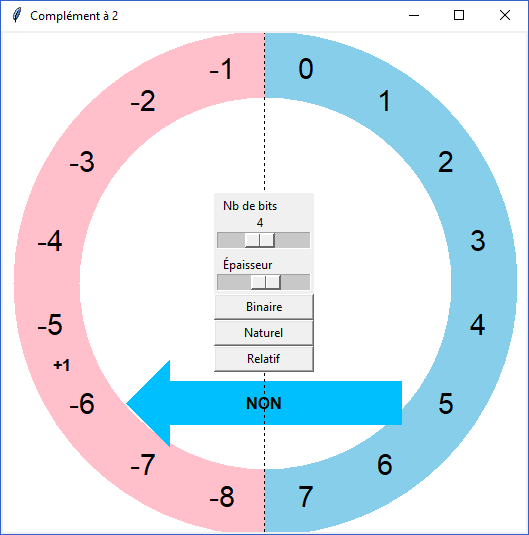
\includegraphics[scale=0.33]{images/complementa2rel.png}\quad
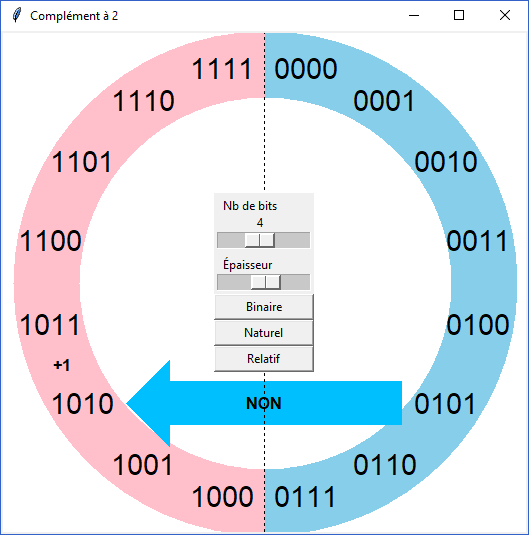
\includegraphics[scale=0.33]{images/complementa2bin.png}
\end{center}

Les nombres binaires et les nombres relatifs sont écrits dans l'ordre en tournant dans le sens des aiguilles d'une montre, tout en conservant la signification du bit de signe. 

Comme on n'a pas de << $-0$ >> il y a un décalage de 1 dans la symétrie entre entiers positifs et négatifs alors qu'elle est parfaite pour les binaires.

\subsection{Complément à 2}

Les résultats précédents permettent de dégager une méthode de codage  :

\begin{center}
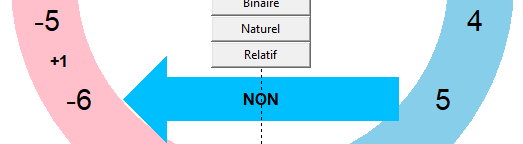
\includegraphics[scale=0.45]{images/complementa2relzoom.png}\quad
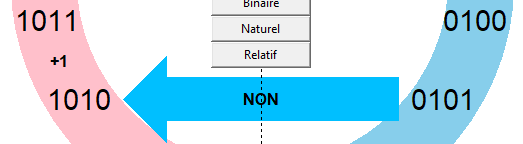
\includegraphics[scale=0.45]{images/complementa2binzoom.png}
\end{center}

Pour coder un entier négatif ($-5$) par complément à 2 sur $n$($=4$) bits, 

\begin{center}\begin{tikzpicture}
\node[draw, text width = 1.5cm,align = center](N)at(-2,2){$-5$};
\node[draw, text width = 1.5cm,align = center](P)at(2,1.5){$5$};
\draw[-latex](N)--(P)node[pos = 0.2, above right, inner sep = 0]{\tikz[baseline=(O.base)]\node[inner sep = 1pt,circle,draw](O){1}; on passe en positif};
\node[draw, text width = 1.5cm,align = center](B1)at(2,0.5){\texttt{0101}};
\draw[-latex](P)--(B1)node[midway, right]{\tikz[baseline=(O.base)]\node[inner sep = 1pt,circle,draw](O){2}; on code en binaire};
\node[draw, text width = 1.5cm,align = center](B2)at(-2,0){\texttt{1010}};
\draw[-latex](B1)--(B2)node[pos = 0.8, below right, inner sep = 0]{\tikz[baseline=(O.base)]\node[inner sep = 1pt,circle,draw](O){3}; on opère une négation de chaque bit};
\node[draw, text width = 1.5cm,align = center](B3)at(-2,1){\texttt{1011}};
\draw[-latex](B2)--(B3)node[midway, left]{on ajoute 1 \tikz[baseline=(O.base)]\node[inner sep = 1pt,circle,draw](O){4};};
\path(B3)--(N)node[midway,sloped]{$=$}; 
\end{tikzpicture}\end{center}

Pour décoder un nombre binaire (\texttt{1011}), on peut suivre un cycle similaire :

\begin{center}\begin{tikzpicture}
\node[draw, text width = 1.5cm,align = center](B1)at(-2,1.5){\texttt{1011}};
\node[draw, text width = 1.5cm,align = center](B2)at(2,2){\texttt{0100}};
\draw[-latex](B1)--(B2)node[pos = 0.8,above left, inner sep = 0]{on opère une négation  de chaque bit \tikz[baseline=(O.base)]\node[inner sep = 1pt,circle,draw](O){1};};
\node[draw, text width = 1.5cm,align = center](B3)at(2,1){\texttt{0101}};
\draw[-latex](B2)--(B3)node[midway, right]{\tikz[baseline=(O.base)]\node(O)[inner sep = 1pt,circle,draw]{2}; on ajoute 1};
\node[draw, text width = 1.5cm,align = center](P)at(2,0){$5$};
\draw[-latex](B3)--(P)node[midway, right]{\tikz[baseline=(O.base)]\node[inner sep = 1pt,circle,draw](O){3}; on décode l'entier positif};
\node[draw, text width = 1.5cm,align = center](N)at(-2,0.5){$-5$};
\draw[-latex](P)--(N)node[pos = 0.2, below left, inner sep = 0]{on passe en négatif \tikz[baseline=(O.base)]\node[inner sep = 1pt,circle,draw](O){4};};
\path(B1)--(N)node[midway,sloped]{$=$}; 
\end{tikzpicture}\end{center}

En fait, pour coder l'entier $-5$, on cherche le nombre $n$ qui vérifie $n+5=0$

\begin{center}\begin{tabular}{cccccl}
{\footnotesize {\footnotesize $1$}} & {\footnotesize $1$} & {\footnotesize $1$} & {\footnotesize $1$} &  & {\footnotesize $\leftarrow$ retenues}\\
 & $0$ & $1$ & $0$ & $1$ &  $\leftarrow 5$\\
$+$ & $1$ & $0$ & $1$ & $1$ & $\leftarrow -5$\\
\cline{1-5}
$(1)$ & $0$ & $0$ & $0$ & $0$ & $\leftarrow 16=2^4$\\
\end{tabular}\end{center}

D'un point de vue des écritures binaires, cela revient à provoquer une retenue qui dépasse le nombre $n$ de bits de l'écriture pour n'obtenir (lui mis à part) que des bits à 0 : on cherche le nombre $n$ qui vérifie $n+5=2^4$ c'est à dire le complément de $5$ à $2^4$.

\Cours{{\bfseries Complément à 2}

L'écriture d'un nombre binaire négatif $m$ en complément à 2 sur $n$ bits est l'écriture binaire du nombre positif $p$ tel que $p + (-m) = 2^n$, c'est à dire, le complément à $2^n$ de $-m$.
}

\subsection{Nombre de bits nécessaires aux opérations}

Un nombre codé sur $n$ bits peut s'écrire de $2^n$ façons. $n$ bits permettent donc de coder 
 tous les {\bfseries entiers naturels} de $\texttt{00...0}_{2}=0$ à $\texttt{11...1}_{2}=2^n-1$.

\begin{center}
\begin{tabular}{ccc}
codage en & plus grand entier  & exemple\\
\hline
8 bits  = 1 octet & \np{255} & primaire RVB \\
16 bits  = 2 octets & \np{65535} & \\
24 bits  = 3 octets & \np{16777215} & couleur RVB \\
32 bits  = 4 octets & \np{4294967295} & IPv4\\
64 bits  = 8 octets & \np{18446744073709551615} & SE actuels \\
\end{tabular}
\end{center}

	Comme $1_2=2^0$, $10_2=2^1$, $100_2=2^2$, $1000_2=2^3$, $10000_2=2^4$, ... 
	
	\begin{center}
	
	Un nombre $n$ a au plus $k$ bits significatifs si et seulement si $n < 2^k$.
	
	\end{center}
	
	({\bfseries Pour aller plus loin : } Il existe une fonction mathématique définissant le réel $y$ tel que $n = 2^y$. Il s'agit de $\text{log}_2$, le logarithme à base 2 : $n = 2^{\text{log}_2(n)}$.)
	
	\begin{itemize}
		\item Additionner deux entiers naturels $n$ et $p$ avec au plus $k$ bits significatifs en nécessite au plus $k+1$ (en effet :  $n < 2^k$ et  $p < 2^k$ donnent  $n + p < 2^k + 2^k = 2\times 2^k = 2^{k+1}$)
		
		(Ce << $+1$ >> correspondant à une éventuelle retenue.)
		\item Multiplier deux entiers naturels $n$ et $p$ avec respectivement au plus $k$ et $l$ bits significatifs en nécessite au plus $k+l$ (en effet :  $n < 2^k$ et  $p < 2^l$ donnent  $n \times p < 2^k \times 2^l = 2^{k+l}$)
	\end{itemize}
	
	\medskip
	
	Un nombre codé sur $n$ bits peut s'écrire de $2^n$ façons. $n$ bits permettent donc de coder 
 tous les {\bfseries entiers relatifs} de $\texttt{10...0}_{2}=-2^{n-1}$ à $\texttt{01...1}_{2}=-2^{n-1}-1$.

\begin{center}
\begin{tabular}{ccc}
codage en & plus petit entier & plus grand entier \\
\hline
8 bits  =  1 octet & \np{-128} & \np{127} \\
16 bits  = 2 octets & \np{-32768} & \np{32 767}\\
32 bits  = 4 octets & \np{-2147483648} & \np{2147483647}\\
64 bits = 8 octets & \np{-9223372036854775808} & \np{9223372036854775807} \\
\end{tabular}
\end{center}

	\begin{itemize}
		\item Additionner un négatif avec un positif ne pose jamais de problème.
		\item Ajouter deux positifs trop grands risque de donner un résultat négatif.
		
		(la retenue se déportant sur le bit de signe.)
		\item Ajouter deux négatifs trop grands risque de donner un résultat positif (même raison).
	\end{itemize}
	
	Il est difficile de mettre en évidence ces dépassements avec Python qui définit des entiers de taille arbitraire. On peut en avoir un aperçu avec la calculatrice de windows en mode programmeur, si on essaie de calculer $\np{9223372036854775807}+1$ on trouve $\np{-9223372036854775808}$, les entiers relatifs étant codés sur 64 bits.

\section{Codage des << réels >>}

Les nombres irrationnels (comme $\sqrt{2}$ ou $\pi$) \emph{ne} peuvent \emph{pas} être représentés car ils contiennent une infinité de chiffres significatifs sans répétition pour les décrire. Et même si c'était possible, n'importe quel intervalle, aussi petit soit-il, contient une infinité de réels donc impossible à distinguer avec un nombre fini de bits. Tout ce que l'on peut faire, c'est coder quelques nombres rationnels choisis.

\subsection{Codage en virgule flottante}

{\bfseries L'écriture décimale} d'un nombre se fait en deux parties finies séparées par une virgule. Par exemple : $\np{324.125} = 3\times 10^2 + 2\times 10^1 + 4\times 10^0 + 1\times 10^{-1} + 2\times 10^{-2} + 5\times 10^{-3}$.

On peut utiliser la même notation en binaire : 

$\np{101.001}_2 = 1\times 2^2 + 0\times 2^1 + 1\times 10^0  + 0\times 2^{-1} + 0\times 2^{-2} + 1\times 2^{-3} (= \np{5.125})$

\medskip

{\bfseries L'écriture scientifique} permet de standardiser l'écriture décimale : $\np{324.125} = \np{3.24125}\times 10^2$

L'avantage pour un nombre binaire ($\neq0$), est que le premier chiffre est toujours 1. Par exemple $101,001_2 = 1,01001_2 \times 10_2\,^{10_2}$. On parle d'écriture normalisée. Il suffit donc de se souvenir de la mantisse (chiffres après la virgule) et de l'exposant. Sans entrer plus dans les détails, voilà comment on procède :

\begin{tikzpicture}[scale=0.5]
\node[](N){\strut Écriture normalisée :~};
\node[draw, right, inner sep = 2pt](S)at(N.east){\strut\texttt{+}};
\node[right, inner sep = 1pt](U)at(S.east){\texttt{1},};
\node[draw, right, inner sep = 2pt](M)at(U.east){\strut\texttt{0100}\,\texttt{1}};
\node[right, inner sep = 1pt](P)at(M.east){\strut $\times 10$};
\node[draw, right, inner sep = 2pt](E)at(P.east){\strut $^{10}$};
%
\node[below left=0.5cm, inner sep = 2pt](C)at(N.south){\strut Codage d'un double (64 bits) :~};
\node[draw, right, inner sep = 2pt](CS)at(C.east){\strut 1 bit : signe};
\node[draw, right, inner sep = 2pt](CE)at(CS.east){\strut 11 bits : exposant};
\node[draw, right, inner sep = 2pt](CM)at(CE.east){\strut 52 bits : mantisse};
%
\draw[-latex](S)to[out=-90, in=90](CS);
\draw[-latex](M)to[out=-45, in=135](CM);
\draw[-latex](E)to[out=-135, in=60](CE);
\end{tikzpicture}

\subsection{Problème d'arrondis}

On peut coder la partie décimale d'un nombre par soustractions successives des puissances de 2 d'exposant négatifs :

\begin{tabular}{c@{\,$=$\,}c@{\,$+$\,}l@{\, donc : \,}l}
$\np{0.625}$ & $\np{0.125}$ & $1\times2^{-1}$ & $\np{0.625}= \texttt{0,1?...}_2$\\

$\np{0.125}$ & $\np{0.125}$ & $0\times2^{-2}$ & $\np{0.625}= \texttt{0,10?...}_2$\\

$\np{0.125}$ & $0$ & $1\times2^{-3}$ & $\np{0.625}= \texttt{0,101}_2$\\
\end{tabular}

Si on essaie de déterminer l'écriture binaire de \np{0.1} :

\begin{tabular}{c@{\,$=$\,}c@{\,$+$\,}l@{\, donc : \,}l}
$\np{0.1}$ & $\np{0.0375}$ & $1\times2^{-4}$ & $\np{0.1}= \texttt{0,0001?...}_2$\\

$\np{0.0375}$ & $\np{0.00625}$ & $1\times2^{-5}$ & $\np{0.1}= \texttt{0,00011?...}_2$\\

$\np{0.00625}$ & $\np{0.00625}$ & $0\times2^{-6}$ & $\np{0.1}= \texttt{0,000110?...}_2$\\

$\np{0.00625}$ & $\np{0.00625}$ & $0\times2^{-7}$ & $\np{0.1}= \texttt{0,0001100?...}_2$\\

$\np{0.00625}$ & $\np{0,00234375}$ & $1\times2^{-8}$ & $\np{0.1}= \texttt{0,00011001?...}_2$\\

$\np{0,00234375}$ & $\np{0,000390625}$ & $1\times2^{-9}$ & $\np{0.1}= \texttt{0,000110011?...}_2$\\

$\np{0,000390625}$ & $\np{0,000390625}$ & $0\times2^{-10}$ & $\np{0.1}= \texttt{0,0001100110?...}_2$\\

$\np{0,000390625}$ & $\np{0,000390625}$ & $0\times2^{-11}$ & $\np{0.1}= \texttt{0,00011001100?...}_2$\\

$\np{0,000390625}$ & $\np{0,000146484375}$ & $1\times2^{-12}$ & $\np{0.1}= \texttt{0,000110011001?...}_2$\\
\end{tabular}

... $\np{0.1}= \texttt{0,0001100110011001100110011001100110011001100110011001100110011...}_2$

Donc \np{0.1} \emph{n'}est \emph{pas} représentable par le codage binaire en virgule flottante !

L'écriture en Python : \pythoninline{x = 0.1} fait donc un arrondi (56 bits après la virgule).

Il n'est donc pas étonnant d'obtenir des résultats approchés par ce codage :

\pythoninline{print(0.1 + 0.2)} affiche \pythoninline{0.30000000000000004}

\pythoninline{print(0.1 + 0.2 == 0.3)} affiche \pythoninline{False}

Ce n'est donc \emph{jamais} une bonne idée de faire des tests d'égalité avec des nombres à virgules flottantes. On préfèrera toujours, quand c'est possible, utiliser des entiers.



\chapter{Expressions booléennes}

\section{Valeurs booléennes}
L'ensemble des booléens comporte exactement deux valeurs : << vrai >> ou << faux >>.

Le type \pythoninline{bool} de Python les note \pythoninline{True} et \pythoninline{False}.

Les variables booléennes servent aux instructions conditionnelles.

\begin{multicols}{2}
\begin{minted}{python3}
if test :
    print('Le test est vrai')
else :
    print('Le test est faux')
\end{minted}  


\begin{minted}{python3}
while test :
    print('Le test est vrai')
    fait_un_truc()
\end{minted}  
\end{multicols}

Les autres types peuvent aussi être évalués comme un booléen :

\begin{minted}{python3}
for test in [True, False, 0, 1, 127, '0', 0.0, 12.34, [], [0], print] :
    if test:
        print(type(test),test,"= vrai.")
    else :
        print(type(test),test,"= faux.")
\end{minted}

\begin{itemize}
	\item {\bfseries FAUX} : \pythoninline{False}, $0$ ou vide.
	\item {\bfseries VRAI} : Tout le reste (ce qui n'est pas faux est vrai).
\end{itemize}

Pour simplifier nous confondrons en particulier \pythoninline{False} avec $0$ et \pythoninline{True} avec $1$.

Dans un souci de lisibilité, on évitera d'écrire des conditionnelles d'un autre type.

\section{Opérateurs booléens}

Comme il n'y a que deux valeurs booléennes, il suffit, pour décrire n'importe quelle fonction ou opérateur booléen, de dresser son tableau de valeurs, appelé : {\bfseries table de vérité}.

\subsection{Une variable}

Il n'existe que $2^2=4$ tables de vérité portant sur une seule variable :

\begin{multicols}{4}

\begin{tabular}{c|cc}
$a$ & \texttt{0} & \texttt{1} \\
\hline
$f_0(a)$ & \texttt{0} & \texttt{0} \\
\end{tabular}


\begin{tabular}{c|cc}
$a$ & \texttt{0} & \texttt{1} \\
\hline
$f_1(a)$ & \texttt{0} & \texttt{1} \\
\end{tabular}


\begin{tabular}{c|cc}
$a$ & \texttt{0} & \texttt{1} \\
\hline
$f_2(a)$ & \texttt{1} & \texttt{0} \\
\end{tabular}


\begin{tabular}{c|cc}
$a$ & \texttt{0} & \texttt{1} \\
\hline
$f_3(a)$ & \texttt{1} & \texttt{1} \\
\end{tabular}

\end{multicols}

$f_0 = 0$ et $f_3 = 1$ et $f_1(a)=a$ n'ont pas besoin d'être nommées pour être utilisées.

$f_2$ par contre permet d'échanger \pythoninline{True} et \pythoninline{False} : c'est une négation.

Python la note \pythoninline{not} et elle s'utilise sans parenthèses. L'équivalent binaire est \pythoninline{~}.

\begin{center}
\begin{tabular}{c|cc}
\pythoninline{a} & \pythoninline{False} & \pythoninline{True} \\
\hline
\pythoninline{not a} & \pythoninline{True} &  \pythoninline{False} \\
\end{tabular} \qquad \qquad
\begin{tabular}{c|cc}
\pythoninline{a} & \pythoninline{0b0} & \pythoninline{0b1} \\
\hline
\pythoninline{~a} & \pythoninline{0b1} &  \pythoninline{0b0} \\
\end{tabular} 
\end{center}

\subsection{Deux variables}

Il existe $2^4=16$ fonctions à 2 variables booléennes. Les trois plus utilisées sont :

\begin{tabular}{c|cccc}
$a$ & \texttt{0} & \texttt{0} & \texttt{1} & \texttt{1} \\
$b$ & \texttt{0} & \texttt{1} & \texttt{0} & \texttt{1} \\
\hline
{\bfseries et}& \texttt{0} & \texttt{0} & \texttt{0} & \texttt{1} \\
\end{tabular} \qquad
\begin{tabular}{c|cccc}
$a$ & \texttt{0} & \texttt{0} & \texttt{1} & \texttt{1} \\
$b$ & \texttt{0} & \texttt{1} & \texttt{0} & \texttt{1} \\
\hline
{\bfseries ou}& \texttt{0} & \texttt{1} & \texttt{1} & \texttt{1} \\
\end{tabular} \qquad
\begin{tabular}{c|cccc}
$a$ & \texttt{0} & \texttt{0} & \texttt{1} & \texttt{1} \\
$b$ & \texttt{0} & \texttt{1} & \texttt{0} & \texttt{1} \\
\hline
{\bfseries ou exclusif}& \texttt{0} & \texttt{1} & \texttt{1} & \texttt{0} \\
\end{tabular}

Python note << et >> : \pythoninline{and} et << ou >> : \pythoninline{or}, mais n'a pas de notation dédiée au << ou exclusif >>. Les équivalents binaires sont respectivement \pythoninline{&}, \pythoninline{|} et \pythoninline{^}.



\begin{center}
\begin{tabular}{c|cccc}
\pythoninline{a} & \pythoninline{False} & \pythoninline{False} & \pythoninline{True} & \pythoninline{True} \\
\pythoninline{a} & \pythoninline{False} & \pythoninline{True} & \pythoninline{False} & \pythoninline{True} \\
\hline
\pythoninline{a and b} & \pythoninline{False} &  \pythoninline{False} & \pythoninline{False} &  \pythoninline{True} \\
\end{tabular} \quad
\begin{tabular}{c|cccc}
\pythoninline{a} & \pythoninline{0b0} & \pythoninline{0b0} & \pythoninline{0b1} & \pythoninline{0b1} \\
\pythoninline{b} & \pythoninline{0b0} & \pythoninline{0b1} & \pythoninline{0b0} & \pythoninline{0b1} \\
\hline
\pythoninline{a & b} & \pythoninline{0b0} &  \pythoninline{0b0} & \pythoninline{0b0} &  \pythoninline{0b1} \\
\end{tabular}

\medskip

\begin{tabular}{c|cccc}
\pythoninline{a} & \pythoninline{False} & \pythoninline{False} & \pythoninline{True} & \pythoninline{True} \\
\pythoninline{a} & \pythoninline{False} & \pythoninline{True} & \pythoninline{False} & \pythoninline{True} \\
\hline
\pythoninline{a or b} & \pythoninline{False} &  \pythoninline{True} & \pythoninline{True} &  \pythoninline{True} \\
\end{tabular} \quad
\begin{tabular}{c|cccc}
\pythoninline{a} & \pythoninline{0b0} & \pythoninline{0b0} & \pythoninline{0b1} & \pythoninline{0b1} \\
\pythoninline{b} & \pythoninline{0b0} & \pythoninline{0b1} & \pythoninline{0b0} & \pythoninline{0b1} \\
\hline
\pythoninline{a | b} & \pythoninline{0b0} &  \pythoninline{0b1} & \pythoninline{0b1} &  \pythoninline{0b1} \\
\end{tabular}

\medskip

\begin{tabular}{c|cccc}
\pythoninline{a} & \pythoninline{0b0} & \pythoninline{0b0} & \pythoninline{0b1} & \pythoninline{0b1} \\
\pythoninline{b} & \pythoninline{0b0} & \pythoninline{0b1} & \pythoninline{0b0} & \pythoninline{0b1} \\
\hline
\pythoninline{a ^ b} & \pythoninline{0b0} &  \pythoninline{0b1} & \pythoninline{0b1} &  \pythoninline{0b0} \\
\end{tabular}
\end{center}

\pythoninline{not}, \pythoninline{and} et \pythoninline{or} sont appelés {\bfseries opérateurs logiques}.

\pythoninline{~}, \pythoninline{&}, \pythoninline{|}, \pythoninline{^} sont des {\bfseries opérateurs  binaires}.

Comme les booléens sont identifiés aux binaires 0 et 1, on peut utiliser  \pythoninline{^}.

\pythoninline{True ^ True} vaut bien \pythoninline{False}, \pythoninline{True ^ False} vaut bien \pythoninline{True}, etc...

Mais il faut faire attention aux priorités de calcul. Le calcul binaire est prioritaire par rapport au calcul booléen. Dans le doute : surcharger de parenthèses ; ne pas mélanger les types ; ou passer par une fonction (dont l'évaluation est encore plus prioritaire mais qui oblige les parenthèses).

\begin{multicols}{2}

On pourra par exemple définir une fonction \pythoninline{xor()} pour les booléens (ci-contre).

\begin{minted}{python3}
def xor(a, b):
    return a ^ b
\end{minted}

\end{multicols}

\section{Caractère séquentiel des opérateurs logiques}

Pour évaluer \pythoninline{a and b}, Python évalue d'abord \pythoninline{a}. 

\begin{itemize}
	\item S'il est \pythoninline{False}, quelque soit \pythoninline{b}, la réponse sera \pythoninline{False}, donc \pythoninline{b} n'est pas évalué.
	
	C'est très pratique, par exemple quand on veut évaluer une valeur d'un tableau :
	
	\pythoninline{if i < len(T) and T[i] > 0 :} si l'indice sort du tableau, \pythoninline{T[i]} ne sera pas évalué.
	
	\item S'il est \pythoninline{True}, \pythoninline{b} détient la réponse : c'est sa valeur qui est renvoyée (sans être testée).
	
	Cela permet un autre raccourci d'écriture : 
	
	\pythoninline{b =  0 <= i < len(T) and T[i]} vaut \pythoninline{False} si \pythoninline{i} sort du tableau et \pythoninline{T[i]} sinon.
\end{itemize}

\begin{multicols}{2}

Grossièrement \pythoninline{a and b} revient à :

\begin{minted}{python3}
def et(a,b):
    if a :
        resultat = b
    else :
        resultat = False
    return resultat
\end{minted}

De même,  \pythoninline{a or b} revient à :

\begin{minted}{python3}
def ou(a,b):
    if a :
        resultat = True
    else :
        resultat = b
    return resultat
\end{minted}

\end{multicols}

On voit en particulier que \pythoninline{a and b} et \pythoninline{b and a} n'ont pas vraiment la même signification (alors que \pythoninline{a & b} et \pythoninline{b & a} si, en binaire)

En utilisant ces deux opérateurs, on arrive parfois à des instructions conditionnelles très courtes (qui ne sont spécialement à rechercher mais à savoir lire) comme :  

\pythoninline{parite = x % 2 == 0 and "pair" or "impair"}


\section{Expressions booléennes}

Une expression booléenne est une expression dont les variables sont booléennes, les opérateurs << non >>,  << ou >> et  << et >> avec éventuellement des parenthèses pour les priorités.

Exemple : \pythoninline{a and not b or not a and b}

Comme toute variable ne peut prendre que 2 valeurs, on peut toujours dresser un tableau de valeurs complet d'une expression booléenne, appelée table de vérité. 

{\bfseries Priorité : } \pythoninline{not} puis \pythoninline{and} puis \pythoninline{or}.

{\centering
\begin{tabular}{c|cccc}
\pythoninline{a} & \texttt{0} & \texttt{0} & \texttt{1} & \texttt{1} \\
\pythoninline{b} & \texttt{0} & \texttt{1} & \texttt{0} & \texttt{1} \\
\hline
\pythoninline{not a} & \texttt{1} & \texttt{1} & \texttt{0} & \texttt{0} \\
\pythoninline{not b} & \texttt{1} & \texttt{0} & \texttt{1} & \texttt{0} \\
\hline
\pythoninline{a and not b} & \texttt{0} & \texttt{0} & \texttt{1} & \texttt{0} \\
\pythoninline{not a and b} & \texttt{0} & \texttt{1} & \texttt{0} & \texttt{0} \\
\hline
\pythoninline{a and not b or not a and b}& \texttt{0} & \texttt{1} & \texttt{1} & \texttt{0} \\
\end{tabular}\par}

Donc \pythoninline{a and not b or not a and b} est une  expression booléenne du << ou exclusif >>.

\medskip

Les {\bfseries règles de calculs} (pour \pythoninline{a} et \pythoninline{b} booléens) :

\begin{multicols}{2}\begin{itemize}
	\item Associativité : 
	
	\pythoninline{(a or b) or c} =  \pythoninline{a or (b or c)}
	
	\pythoninline{(a and b) and c} = \pythoninline{a and (b and c)}
    \item Commutativité : 
    
    \pythoninline{a or b} = \pythoninline{b or a}
    
    \pythoninline{a and b} = \pythoninline{b and a}
    \item Distributivité :
    
     \pythoninline{(a or b) and c} 
     
     \qquad = \pythoninline{(a and c) or (b and c)} 
     
     \pythoninline{(a and b) or c} 
     
     \qquad = \pythoninline{(a or c) and (b or c)}
     
     \columnbreak
    \item Élément neutre : 
    
    \pythoninline{a or False} = \pythoninline{a}
    
    \pythoninline{a and True} = \pythoninline{a}
    \item Élément absorbant : 
    
    \pythoninline{a or True} = \pythoninline{True}
    
    \pythoninline{a and False} = \pythoninline{False}
    \item Négation : 
    
    \pythoninline{a or not a} = \pythoninline{True}
    
    \pythoninline{a and not a} = \pythoninline{False}
    \item Loi de De Morgan : 
    
    \pythoninline{not (a or b)} = \pythoninline{not a and not b}
    
    \pythoninline{not (a and b)} = \pythoninline{not a or not b}
\end{itemize}\end{multicols}

\section{Application au calcul binaire}

On écrit ici $1$ pour \pythoninline{True} et $0$ pour \pythoninline{False} et on va réécrire les opérations binaires avec des formules logiques. Posons les additions à un bit :

\begin{center}
\begin{multicols}{5}
\begin{tabular}{c@{\,}c@{\,}c}
    &   & $0$ \\
$+$ &   & $0$ \\
\hline
    &   & $0$\\
\end{tabular}


\begin{tabular}{c@{\,}c@{\,}c}
    &   & $1$ \\
$+$ &   & $0$ \\
\hline
    &   & $1$\\
\end{tabular}


\begin{tabular}{c@{\,}c@{\,}c}
    &   & $0$ \\
$+$ &   & $1$ \\
\hline
    &   & $1$\\
\end{tabular}


\begin{tabular}{c@{\,}c@{\,}c}
    &   & $1$ \\
$+$ &   & $1$ \\
\hline
    &$1$& $0$\\
\end{tabular}


\begin{tabular}{c@{}c@{}c}
    &   & \pythoninline{a} \\
$+$ &   & \pythoninline{b} \\
\hline
    &\pythoninline{r}& \pythoninline{s}\\
\end{tabular}
\end{multicols}
\end{center}

Il n'y a une retenue que si les deux bits sont à 1 : \pythoninline{r = a and b}

Sans la retenue, le résultat est 1 seulement si un seul bit est 1 : \pythoninline{s = xor(a,b)}

\medskip
Pour additionner deux entiers écrits en binaire, il est nécessaire de tenir compte des retenues à chaque addition de deux bits :

\begin{center}
\begin{multicols}{2}
\begin{tabular}{ccccc}
    & {\scriptsize$0$} & {\scriptsize$1$} & {\scriptsize$1$} &   \\
    & $1$ & $0$ & $1$ & $1$ \\
$+$ & $0$ & $0$ & $1$ & $1$ \\
\hline
    & $1$ & $1$ & $1$ & $0$\\
\end{tabular}

\begin{tabular}{c@{}c@{~}c@{~}c@{~}c@{~}c}
&    & \pythoninline[fontsize=\scriptsize]{r2} & \pythoninline[fontsize=\scriptsize]{r1} & \pythoninline[fontsize=\scriptsize]{r0} & \pythoninline[fontsize=\scriptsize]{0}   \\
&   & \pythoninline{a3} & \pythoninline{a2} & \pythoninline{a1} & \pythoninline{a0} \\
\pythoninline{+}& & \pythoninline{b3} & \pythoninline{b2} & \pythoninline{b1} & \pythoninline{b0} \\
\hline
&\pythoninline{r3}    & \pythoninline{s3} & \pythoninline{s2} & \pythoninline{s1} & \pythoninline{s0} \\
\end{tabular}

\end{multicols}
\end{center}

On veut ajouter \pythoninline{r0} à la somme de \pythoninline{a1} et \pythoninline{b1}.

Cela revient à l'ajouter à \pythoninline{xor(a1,b1)} avec une retenue \pythoninline{a1 and b1}.

On trouve donc \pythoninline{xor(r0,xor(a1,b1))} et une retenue si \pythoninline{a1 and b1} ou \pythoninline{r0 and xor(a1,b1))}.

\begin{center} \pythoninline{s1 = xor(r0,xor(a1,b1))} \qquad et \qquad
\pythoninline{r1 = a1 and b1 or r0 and xor(a1,b1)}
\end{center}

\begin{minted}{python3}
def somme1(r,a,b) :
    return a and b or r and xor(a,b), xor(r,xor(a,b))
\end{minted}

La somme de deux binaires serait alors :

\begin{minted}{python3}
def somme(a,b) :
    """ Calcule la somme des binaires a et b 
    
    a et b sont sous la forme de tableaux de booléens de même taille,
    le bit de poids le plus faible en premier"""
    s = []
    r = False
    for k in range(len(a)):
        r, somme = somme1(r,a[k],b[k])
        s.append(somme)
    return r, s
\end{minted}

\chapter{Représentation d'un texte}

\date{1940} À partir du moment où il est clairement apparu que les ordinateurs n'allaient plus servir à traiter que des informations numériques brutes, le problème du codage des caractères s'est posé.

\section{ASCII}
	 
\Cours{{\bfseries ASCII} : American Standart Code for Information Interchange : 


C'est la première norme, adoptée après de nombreuses révisions, par l'<< American National Standards Institute >> (ANSI) dans les années 1960. 
}
 

À l'époque les ordinateurs fonctionnaient en 8 bits, et, 1 bit de parité étant conservé pour la détection des erreurs de transmission, $2^7=128$ caractères étaient suffisants pour coder les lettres majuscules, minuscules, chiffres et ponctuations.

\medskip

Le document ci-dessous date de 1972 :

\begin{center}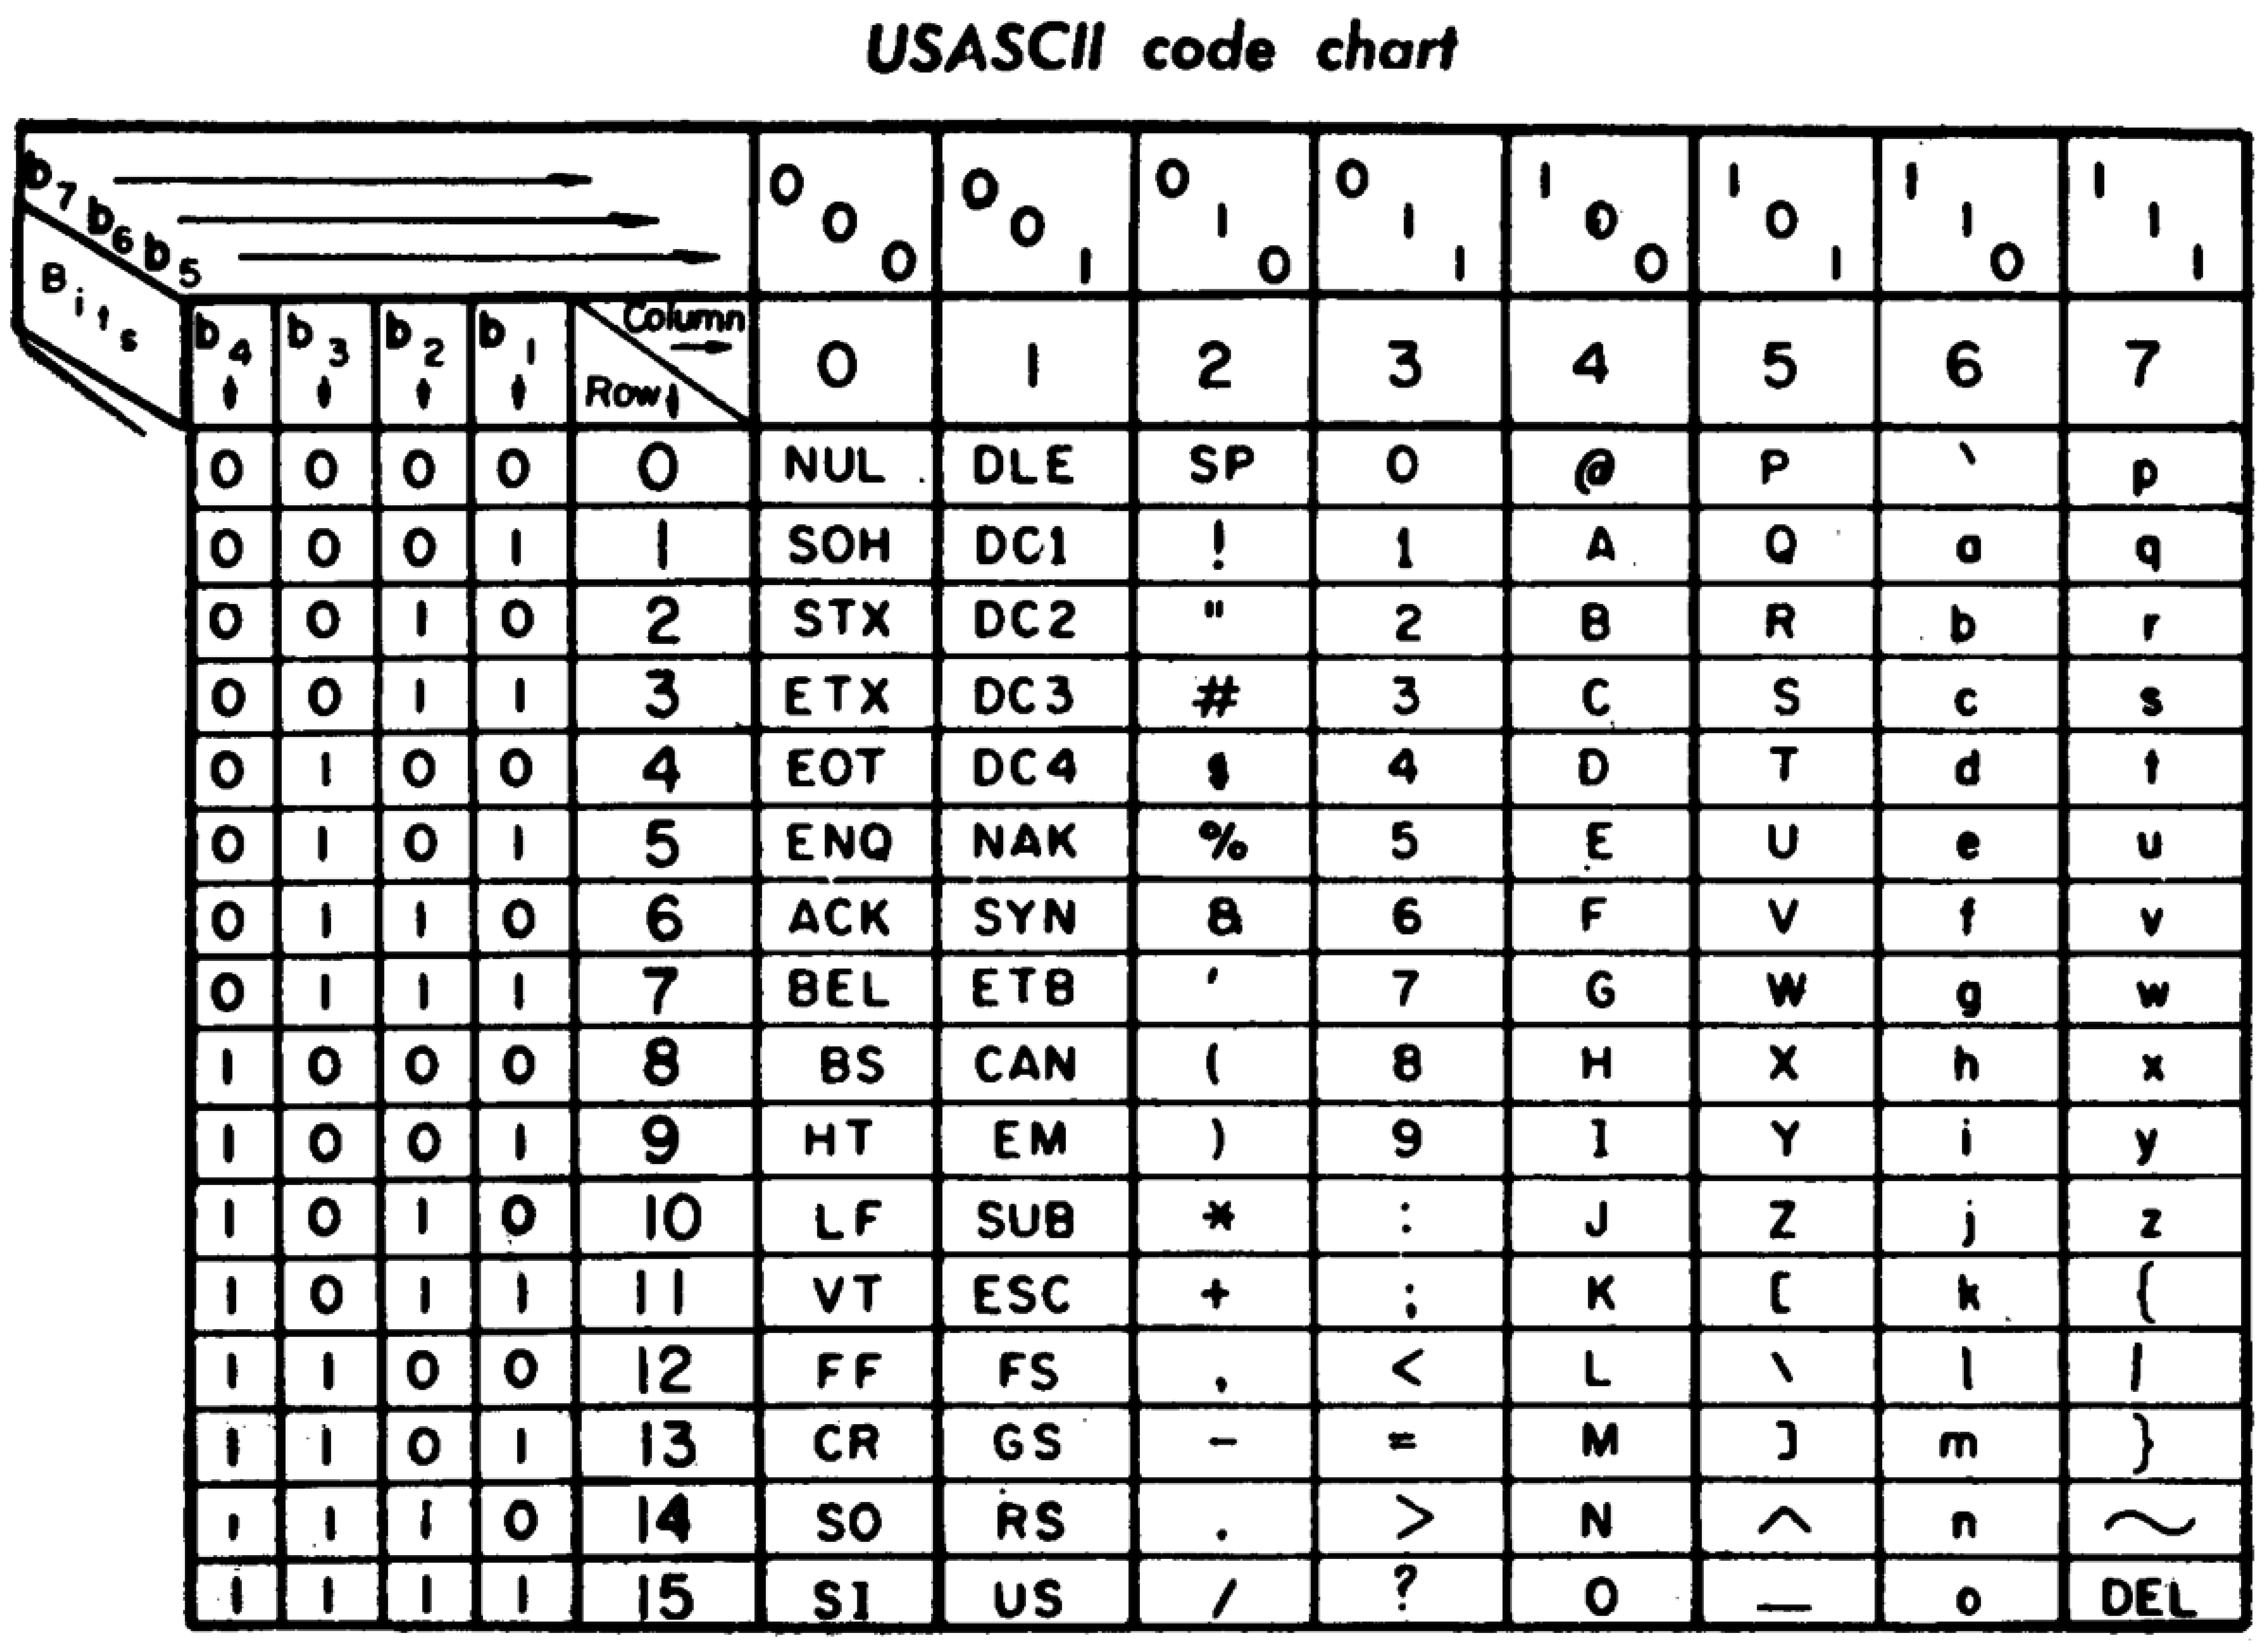
\includegraphics[scale=0.12]{images/US-ASCII_code_chart}

\footnotesize Source : https://en.wikipedia.org/wiki/ASCII\#/media/File:US-ASCII\_code\_chart.png
\end{center}

Par exemple, le caractère \pythoninline{'A'}, est le caractère numéro \mintinline{text}{100 0001}.

C'est-à-dire : \texttt{1}$\times2^6+$\texttt{0}$\times2^5+\ldots+$\texttt{0}$\times2^1+$\texttt{1}$\times2^0=65$ en décimal. 

Le tableau permet d'en lire l'écriture hexadécimale : \texttt{41}.

On peut vérifier par le calcul : \texttt{4}$\times16^1+$\texttt{1}$\times16^0=65$.

\medskip

Comme l'ASCII est la base de notre codage actuel, on obtient donc << A >> indifféremment par \pythoninline{'A'} ou \pythoninline{chr(65)} ou \pythoninline{chr(0x41)} ou encore \pythoninline{chr(0b1000001)}, et son code par \pythoninline{ord('A')}.

\section{Formats ISO}

L'amélioration de la fiabilité des transmissions et les besoins des européens, par exemple d'accentuer les lettres, ont abouti à l'utilisation du 8$^\text{ème}$ bit et donc à doubler le nombre de caractères codés. 
	
\Cours{{\bfseries latin-1}

\medskip C'est la norme ISO 8859-1 pour l'encodage des caractères. Elle contient les caractères accentués utilisés dans les langues latines.
}

On peut citer également :

\begin{itemize}
	\item l'ISO 8859-7 qui contient les caractères grecs.
    \item l'ISO 8859-15 ou latin 9, presque identique au latin 1 à 8 caractères près (le latin 9 contient par exemple les caractères œ, Œ et € qui ne sont pas dans la table latin 1).
\end{itemize}
	
L'encodage utilisé ne fait pas partie du contenu des fichier textes. Si on se trompe sur l'encodage utilisé, certains caractères seront donc mal interprétés. On voit encore apparaître des caractères sur des pages ou courriels dont l'encodage est mal spécifié. La phrase << C'est très raté ! >> par exemple devient << C'est très raté ! >>.

\section{Format Unicode}

\date{1990} Apparaît la norme Unicode, codée sur 2 octets (16 bits), pour réunir tous les caractères dans une seule table. On peut l'utiliser pour notre \pythoninline{'A'} :\pythoninline{'\u0041'}.

\medskip

Cette norme est encore en construction aujourd'hui, et contient actuellement plus de \np{135000} symboles codé sur 21 bits. Le code unicode n'est pas utilisé directement comme encodage de fichiers (sous peine de voir la taille des fichiers texte multipliée par 3). Ce sont des encodages comme UTF-8 qui permettent d'utiliser Unicode. 

\Cours{{\bfseries UTF-8}

\medskip C'est un encodage des caractères sur un seul octet, qui utilise des séquences d'échappement pour accéder à d'autres parties de la table. En UTF-8, tous les caractères n'occupent donc pas la même place. Certains sont codés sur 1 octet, et d'autres sur 2 à 4 octets.
} 

Pour expliquer le problème << C'est très raté ! >>, regardons comment est encodé << è >> :

\pythoninline{'è'.encode('utf8')} donne \pythoninline{b'\xc3\xa8'}.

On voit que le caractère d'échappement a le code hexadécimal : \texttt{C3}.

S'il n'était pas considéré comme échappement il serait \pythoninline{chr(0xc3)} qui donne \pythoninline{Ã}

\medskip

Et pour le << é >> ? 

\pythoninline{'é'.encode('utf8')} donne \pythoninline{b'\xc3\xa9'}. C'est le même échappement.

\medskip

Pour le << € >> il faut aller plus loin, l'échappement est différent : 

\pythoninline{'€'.encode('utf8')} donne \pythoninline{b'\xe2\x82\xac'}.

\medskip

Actuellement, la bonne pratique est d'utiliser UTF-8 dès que c'est possible.

\begin{minted}{python3}
# Supposons que fichier.txt soit encodé en latin1 !
with open('fichier.txt', encoding="latin1") as fichier :
    text = fichier.read()
with open('fichier.txt', mode="w", encoding="utf8") as fichier :
    fichier.write(text)
# Le problème est réglé.
\end{minted}

\partie{Types construits}
\chapter*{Programme officiel}

\section*{Programme officiel}

À partir des types de base se constituent des types construits, qui sont introduits au fur et à mesure qu'ils sont nécessaires.

Il s'agit de présenter tour à tour les p-uplets (tuples), les enregistrements qui collectent des valeurs de types différents dans des champs nommés et les tableaux qui permettent un accès calculé direct aux éléments. En pratique, on utilise les appellations de Python, qui peuvent être différentes de celles d'autres langages de programmation.

{\centering\begin{tabular}{|L{3cm}|L{5.5cm}|L{6cm}|}\hline
\cellcolor{bo}\bfseries\textcolor{white}{Contenus}&
\cellcolor{bo}\bfseries\textcolor{white}{Capacités attendues}&
\cellcolor{bo}\bfseries\textcolor{white}{Commentaires}\\ \hline
p-uplets.

p-uplets nommés
&
Écrire une fonction renvoyant un p-uplet de valeurs.
& \\ \hline
Tableau indexé, tableau donné en compréhension
&
Lire et modifier les éléments d'un tableau grâce à leurs index.

Construire un tableau par compréhension.

Utiliser des tableaux de tableaux pour représenter des matrices : notation a [i] [j].

Itérer sur les éléments d'un tableau.
&
Seuls les tableaux dont les éléments sont du même type sont présentés.

Aucune connaissance des tranches (slices) n'est exigible.

L’aspect dynamique des tableaux de Python n'est pas évoqué. Python identifie listes et tableaux.

Il n'est pas fait référence aux tableaux de la bibliothèque NumPy.\\ \hline
Dictionnaires par clés et valeurs
&
Construire une entrée de dictionnaire.

Itérer sur les éléments d'un dictionnaire.
&
Il est possible de présenter les données EXIF d'une image sous la forme d'un enregistrement.

En Python, les p-uplets nommés sont implémentés par des dictionnaires.

Utiliser les méthodes keys(), values() et items().\\ \hline
\end{tabular}\par}


\chapter{Tableaux indexés}

\section{Définition et lecture}

\Cours{{\bfseries Tableau}

D'un point de vue algorithmique, un \emph{tableau} est une structure de données définie par une séquence finie d'éléments de même type, auxquels on accède par leur position (entière positive) dans la séquence, appelé indice. 
}

Le langage Python n'implémente pas directement ce type. On utilisera le type \pythoninline{list}, plus permissif (par exemple qui autorise des valeurs de types différents).

\begin{itemize}
	\item On peut définir un tableau par la séquence de ses valeurs : \pythoninline{Tableau = [15,18,20]}.
	\item Sa taille est donnée par la fonction \pythoninline{len()} : \pythoninline{len(Tableau)} vaut 3.
	\item On accède à chaque valeur par son indice (entre 0 et 2) : \pythoninline{Tableau[1]} vaut 18.
	\item Ses valeurs sont modifiables (le type tableau est mutable) : \pythoninline{Tableau[1]=12}.
	\item C'est comme si on avait trois variables : \pythoninline{Tableau[0]}, \pythoninline{Tableau[1]} et \pythoninline{Tableau[2]}.
\end{itemize}

\begin{multicols}{2}
Représentation humaine :

\begin{tabular}{|c|c|c|c|}
\hline
Tableau & 15 & 18 & 20 \\
\hline
\end{tabular}

\medskip
Implémentation (liste Python) :

\pythoninline{Tableau = [15,18,20]}.

\columnbreak
Représentation en mémoire :

\begin{tikzpicture}
\node(T){\pythoninline{Tableau}};
\node[inner sep = 5pt, right, draw](Tc)at(T.east){\footnotesize$\bullet$};
\node[inner sep = 5pt, draw, below right = 1.5cm](L0)at(Tc){\footnotesize$\bullet$};
\draw[-latex](Tc.center)to[out = -45, in = 180](L0.west);
\node[inner sep = 1pt, below right]at(L0.north west){\scriptsize\texttt{0}};
\node[inner sep = 1pt, above]at(L0.north){\pythoninline[fontsize=\scriptsize]{list}};
\node[inner sep = 5pt, draw, right = -0.4pt](L1)at(L0.east){\footnotesize$\bullet$};
\node[inner sep = 1pt, below right]at(L1.north west){\scriptsize\texttt{1}};
\node[inner sep = 5pt, draw, right = -0.4pt](L2)at(L1.east){\footnotesize$\bullet$};
\node[inner sep = 1pt, below right]at(L2.north west){\scriptsize\texttt{2}};
\node[inner sep = 0pt,right=2.25cm, yshift=-0.3cm](V0)at(Tc){\pythoninline[fontsize=\footnotesize]{15}};
\node[inner sep = 0pt, above]at(V0.north){\pythoninline[fontsize=\scriptsize]{int}};
\node[inner sep = 0pt,below right=0.3cm, xshift=0.3cm](V1)at(V0){\pythoninline[fontsize=\footnotesize]{18}};
\node[inner sep = 0pt, above]at(V1.north){\pythoninline[fontsize=\scriptsize]{int}};
\node[inner sep = 0pt,below right=0.3cm, xshift=0.3cm](V2)at(V1){\pythoninline[fontsize=\footnotesize]{20}};
\node[inner sep = 0pt, above]at(V2.north){\pythoninline[fontsize=\scriptsize]{int}};
\draw[-latex](L0.center)to[out = 45, in = 180](V0.west);
\draw[-latex](L1.center)to[out = 25, in = 180](V1.west);
\draw[-latex](L2.center)to[out = 5, in = 180](V2.west);
\end{tikzpicture}
\end{multicols}

On peut obtenir des représentations sur : \href{http://pythontutor.com/live.html#mode=edit}{http://pythontutor.com/live.html\#mode=edit}.


\section{Itération}

Pour parcourir les valeurs d'un tableau, on peut utiliser leur indice.

\begin{multicols}{2}
Par exemple le code ci-contre affiche les valeurs du tableau en passant à la ligne après chaque bloc de quatre valeurs.

\begin{minted}{python}
valeur = [0,1,1,0,1,0,1,0,1,0,1,1]
for i in range(len(valeur)):
    print(valeur[i], end = '')
    if i % 4 == 3 : print()
\end{minted}
\end{multicols}

Mais les indices peuvent ne pas avoir d'importance et seulement surcharger l'écriture du code. Dans ce cas, on peut itérer directement sur les éléments du tableau :


\begin{multicols}{2}
Avec les indices :

\vspace{-2ex}
\begin{minted}{python}
valeur = [10,13,15,11,12]
somme = 0
for i in range(len(valeur)):
    somme = somme + valeur[i]
\end{minted}

Sans les indices :

\vspace{-2ex}
\begin{minted}{python}
valeur = [10,13,15,11,12]
somme = 0
for val in valeur:
    somme = somme + val
\end{minted}
\end{multicols}

{\bfseries Pour aller plus loin :} Il peut se produire des cas où l'on aimerait avoir les deux avantages. (Notamment si l'itération ne porte pas sur un tableau mais sur un autre itérable dont on ne sait pas déterminer facilement la taille.) On peut les obtenir avec la syntaxe suivante :


\vspace{-2ex}
\begin{minted}{python}
valeur = [10,13,15,11,12]
for (i,val) in enumerate(valeur):
    print('valeur[', i, '] = ',val, sep='')
\end{minted}

\section{Tableaux en compréhension}

On peut construire une liste Python à l'aide de la méthode \pythoninline{append()}.

\begin{multicols}{2}
Par exemple pour dresser le tableau des 10 premiers carrés d'entiers naturels, on peut écrire le code Python ci-contre.

\begin{minted}{python}
carre = []
for x in range(10):
    carre.append(x ** 2)
\end{minted}
\end{multicols}

Il existe une manière condensée de faire la même chose :\pythoninline{carre = [x**2 for x in range(10)]}

\begin{multicols}{2}
Dans l'exemple ci-contre, on utilise cette façon de faire pour appliquer un traitement à tous les éléments d'un autre tableau.

\begin{minted}{python}
lettres = ['a', 'e', 'i', 'o', 'u']
lettres = [ord(l) for l in lettres]
\end{minted}
\end{multicols}

On peut également imposer une condition à l'inclusion de la valeur : 

\pythoninline{chiffresPairs = [n for n in range(10) if n%2 == 0]}

\Cours{{\bfseries Tableau en compréhension}

On définit un tableau en compréhension en utilisant une description de ses termes.

Avec Python, elle prend la forme suivante :

\pythoninline{[fonction(item) for item in iterable if condition(item)]}

}

\section{Tableau de tableaux}

L'idée des tableaux de tableaux est de pouvoir représenter des tableaux à 2 dimensions. Par exemple, la grille d'un jeu de morpion est une grille $3\times3$. Voici deux codages possibles : \hfill\begin{tikzpicture}[scale=0.66,overlay,xshift = -3cm, yshift=-3.5cm]
\foreach \i in {0,1,2,3} \draw(0,\i)--(3,\i)(\i,0)--(\i,3);
\draw[rouge](1,1)--(2,2)(1,2)--(2,1);
\draw[bleu](1.5,2.5)circle(0.4);
\foreach \i in {1, 2, 3} \node[inner sep = 1pt, below right]at({\i-1},1){\footnotesize \texttt{\i}};
\foreach \i in {4, 5, 6} \node[inner sep = 1pt, below right]at({\i-4},2){\footnotesize \texttt{\i}};
\foreach \i in {7, 8, 9} \node[inner sep = 1pt, below right]at({\i-7},3){\footnotesize \texttt{\i}};
\end{tikzpicture}
\begin{itemize}
	\item On fait correspondre un numéro de case à un indice :
	
	     \pythoninline{[-1,0,0,0,0,1,0,0,2,0]} (1 : joueur 1 et 2 : joueur 2)

    \item On dresse la liste des cases jouées, la parité des indices donne le joueur :
    
        \pythoninline{[5,8,0,0,0,0,0,0,0]}
\end{itemize}

Voici maintenant une autre possibilité, utilisant un tableau de tableaux :\hfill\begin{tikzpicture}[scale=0.66,overlay,xshift = -3cm, yshift=-3.5cm]
\node[]at(1.5,{2.5-0}){\pythoninline{grille[0]}};
\node[]at(1.5,{2.5-1}){\pythoninline{grille[1]}};
\node[]at(1.5,{2.5-2}){\pythoninline{grille[2]}};
\foreach \i in {0,1,2,3} \draw(0,\i)--(3,\i)(\i,0)--(\i,3);
\draw[rouge](1,1)--(2,2)(1,2)--(2,1);
\draw[bleu](1.5,2.5)circle(0.4);
\end{tikzpicture}

\begin{itemize}
	\item La grille est un tableau de lignes  :
	
	\pythoninline{grille[0] = [0,2,0]}, \pythoninline{grille[1] = [0,1,0]},\pythoninline{grille[2] = [0,0,0]}
	
	C'est à dire \pythoninline{grille = [ [0,2,0], [0,1,0], [0,0,0] ]}
	
	Et on accède par exemple à la valeur 2 par : \pythoninline{grille[0][1]}.
	
\end{itemize}

Ce ne sont évidemment pas les seules options (chaque élément du tableau pourrait être une colonne, ou avec des indices dans l'autre sens, etc.)

\medskip
On peut écrire des tableaux de tableaux en compréhension :

\vspace{-2ex}
\begin{minted}{python}
grille = [[3 * ligne + colonne for colonne in range(3)] for ligne in range(3)]
\end{minted}

Et on peut itérer sur ses indices ou ses éléments par une double boucle :

\vspace{-2ex}
\begin{multicols}{2}
\begin{minted}{python}
for i in len(grille) :
    for j in len(grille[i]) :
        grille[i][j] = 0
\end{minted}

\begin{minted}{python}
for ligne in grille :
    for valeur in ligne :
        valeur = 0
\end{minted}
\end{multicols}


\chapter{p-uplets (tuples) et Dictionnaires}

Le chapitre précédent présentait les tableaux : une structure de données de taille fixe, dont les éléments sont de même type, ordonnés et accessibles par leur indice. Comme de plus ils peuvent être modifiés, on dit que c'est un type \emph{mutable}. On utilise les listes pour les représenter car elles ont des propriétés similaires avec certaines restrictions en moins. Mais d'autres types s'adaptent à d'autres situations :

\begin{center}\begin{tabular}{l|c|ccc}
type construit       & tableau & \pythoninline{list} & \pythoninline{tuple} & \pythoninline{dict} \\
\hline
valeurs de même type&\checkmark &  \textsf{X}   &   \textsf{X}   &   \textsf{X}   \\
ordonné et indicé   &\checkmark &  \checkmark   &   \checkmark   &   \textsf{X}   \\
champs nommés       &\textsf{X} &  \textsf{X}   &   \textsf{X}   &   \checkmark   \\
mutable             &\checkmark &  \checkmark   &   \textsf{X}   &   \checkmark   \\
taille fixe         &\checkmark &  \textsf{X}   &   \checkmark   &   \textsf{X}   \\
\end{tabular}\end{center}

Il existe aussi des p-uplets nommés, qui ont les mêmes caractéristiques que les p-uplets mais dont on peut nommer des champs. Dans la pratique au lycée, nous utiliserons préférentiellement les dictionnaires dans ce cas.

\section{p-uplets}

\subsection{Définition}

\Cours{{\bfseries p-uplets}

Un \emph{p-uplet} est une structure de données définie par une séquence finie d'éléments non modifiables, auxquels on accède par leur position (entière positive) dans la séquence, appelé indice.
}

 Un 2-uplet est un couple, par exemple (latitude, longitude). Un 3-uplet est un triplet, par exemple les coordonnées d'un point dans l'espace. Un 4-uplet est un quadruplet, etc.

\subsection{Fonctionnalité}

Le langage Python implémente ce type sous la dénomination \pythoninline{tuple}.

\begin{itemize}
	\item On peut définir un p-uplet par la séquence de ses valeurs : \pythoninline{point = ('A',3)}.
	\item Les parenthèses ne sont pas obligatoires, on peut aussi écrire : \pythoninline{point = 'A',3}.
	\item Pour un 1-uplet, l'absence de virgule ne permettrait pas de savoir si les parenthèses sont de simples parenthèses de calcul, ou la définition d'une structure. Python permet de terminer la séquence de valeurs par une virgule pour lever toute ambiguïté : \pythoninline{point = 'A',3,}, et pour un  1-uplet : \pythoninline{lettre = 'A',}.
	\item Pour un 0-uplet, cette notation ne suffit plus. On utilise alors : \pythoninline{vide = tuple()}.
	\item C'est, pour les mêmes raisons, la notation à utiliser pour une définition en compréhension : \pythoninline{chiffresPairs = tuple(n for n in range(10) if n%2 == 0)}
	\item Sa taille est donnée par la fonction \pythoninline{len()} : \pythoninline{len(point)} vaut 2.
	\item On accède à chaque valeur par son indice : \pythoninline{point[1]} vaut 3.
	\item Ses valeurs ne sont pas modifiables : \pythoninline{point[1]=12} provoquera une erreur.
	\item C'est comme si on avait deux constantes : \pythoninline{point[0]} et \pythoninline{point[1]}.

    \item On peut \emph{itérer} un p-uplet.


\begin{multicols}{2}
Avec les indices :

\vspace{-2ex}
\begin{minted}{python}
valeur = (10,13,15,11,12)
somme = 0
for i in range(len(valeur)):
    somme = somme + valeur[i]
\end{minted}

Sans les indices :

\vspace{-2ex}
\begin{minted}{python}
valeur = (10,13,15,11,12)
somme = 0
for val in valeur:
    somme = somme + val
\end{minted}
\end{multicols}
\end{itemize}

\subsection{Utilisation}

Le fait que ce type ne soit pas mutable peut être la propriété recherchée. 

Cela fait des données des constantes.

\medskip

Les éléments d'un p-uplet peuvent être des noms de variables (ou de fonctions). 

C'est ce qui permet les affections multiples donc les écritures comme :

\vspace{-2ex}
\begin{minted}{python}
x, y = 1, 2 # Le tuple n'est pas mutable, la variable x est toujours la variable x.
x, y = y, x # C'est la valeur que pointe (représente) x qui change !
\end{minted}

\medskip

On utilise cette structure pour permettre à une fonction de renvoyer plusieurs valeurs.

\vspace{-2ex}
\begin{minted}{python}
def divisionEuclidienne(x,y):
    return x//y, x%y
    
quotient, reste = divisionEuclidienne(7,2)
\end{minted}


\medskip
{\bfseries Pour aller plus loin : Unpacking}

On peut aussi vouloir se servir de cette structure pour passer un nombre indéterminé de valeurs à une fonction : 

\vspace{-2ex}
\begin{minted}{python}
def produit(valeurs):
    produit = 1
    for val in valeurs:
        produit = produit * val
    return produit

p = produit((1,2,3))
\end{minted}

Mais cela surcharge l'écriture de l'appel de la fonction.

On utilise alors l'opérateur \emph{splat} \pythoninline{*} pour récupérer les arguments en surnombre dans un seul un p-uplet :

\vspace{-2ex}
\begin{minted}{python}
def produit(*valeurs):
    produit = 1
    for val in valeurs:
        produit = produit * val
    return produit

p = produit(1,2,3)
\end{minted}

Dans l'appel de chacune des fonctions précédentes, la variable locale \pythoninline{valeurs} vaut la même chose : le triplet \pythoninline{(1,2,3)}.

\medskip

Cet opérateur permet de << dépacker >> un tuple. Si par exemple on dispose d'un n-uplet et qu'on souhaite l'utiliser pour les dernières valeurs d'un (n+1)-uplet :

\vspace{-2ex}
\begin{minted}{python}
coord = (3, -5)
point = ('A',*coord)  # revient à point = ('A', 3, -5)
\end{minted}

\section{Dictionnaires}

\subsection{Définition}

\Cours{{\bfseries Dictionnaire}

Un dictionnaire est une structure de données définie par un ensemble d'éléments, auxquels on accède par mot clé.}

Exemple : \pythoninline{{'nom' : 'A', 'x' : 3, 'y' :-5}} ou \pythoninline{{'nom' : 'A', 'coord' : (3, -5)}} ou encore \pythoninline{{(3, -5) : 'A'}}...

\subsection{Fonctionnalité}

Le langage Python implémente ce type sous la dénomination \pythoninline{dict}.

\begin{itemize}
	\item il est défini par l'ensemble de ses éléments (clé : valeurs) : \pythoninline{point = {'x' : 3, 'y' :-5}}. Une clé doit être unique (une clé comme un indice de liste ne référence qu'une valeur).
	\item Le dictionnaire vide s'écrit : \pythoninline{vide = dict()}.
	\item Un dictionnaire en compréhension s'écrit : \pythoninline{{n : n ** 3 for n in range(10) if n > 0}}
	\item Sa taille est donnée par la fonction \pythoninline{len()} : \pythoninline{len(point)} vaut 2.
	\item La liste des clés est \pythoninline{list(point.keys())}.
	\item La liste des valeurs est \pythoninline{list(point.values())}.
	\item La liste des couples (clé, valeur) est \pythoninline{list(point.items())}.
	\item On accède à chaque valeur par sa clé : \pythoninline{point['x']} vaut 3.
	
	Si une clé peut ne pas être présente, on utilise la méthode \pythoninline{get()} :
	
	 \pythoninline{point.get('z',0)]} renvoie \pythoninline{point['z']} si \pythoninline{'z'} est bien une clé ;  \pythoninline{0} sinon (par défaut).
	 
	 ( On peut tester la présence d'une clé avec la méthode \pythoninline{has_key()}. )
	 
	\item C'est comme si on avait plusieurs variables : \pythoninline{point['x']}, \pythoninline{point['y']}.

    \item On peut \emph{itérer} un dictionnaire par ses clés :


\begin{multicols}{2}
De manière implicite :

\vspace{-2ex}
\begin{minted}{python3}
for clef in point :
    print(clef, ':', point[clef])
\end{minted}

De manière explicite :

\vspace{-2ex}
\begin{minted}{python3}
for clef in point.key() :
    print(clef, ':', point[clef])
\end{minted}
\end{multicols}

\begin{multicols}{2}
    \item On peut itérer sur les valeurs :
    
\vspace{-2ex}
\begin{minted}{python3}
for valeur in point.values() :
    print(valeur)
\end{minted}

    \item On peut itérer sur les éléments :
    
\vspace{-2ex}
\begin{minted}{python3}
for clef, valeur in point.items() :
    print(clef, ':', valeur)
\end{minted}
    
\end{multicols}
\end{itemize}

\subsection{Exemple d'utilisation}

Cet exemple suppose que la bibliothèque \mintinline{text}{pillow} soit installée, et la présence d'une image dans le dossier de travail.

Les données EXIF d'une image sont de la forme \mintinline{text}{clé-numérique : valeur}.

Pillow contient un dictionnaire \pythoninline{TAGS} d'éléments  \mintinline{text}{clé-numérique : signification}.

\begin{minted}{python3}
from PIL import Image
from PIL.ExifTags import TAGS
 
with Image.open('image.jpg') as img:
    exif = img._getexif()
    for tag in exif :
        print(TAGS.get(tag, tag),':',exif[tag])
\end{minted}



\partie{Traitement de données en tables}
\chapter*{Programme officiel}

\section*{Programme officiel}

Les données organisées en table correspondent à une liste de p-uplets nommés qui partagent les mêmes descripteurs. La mobilisation de ce type de structure de données permet de préparer les élèves à aborder la notion de base de données qui ne sera présentée qu'en classe terminale. Il s'agit d'utiliser un tableau doublement indexé ou un tableau de p-uplets, dans un langage de programmation ordinaire et non dans un système de gestion de bases de données.

{\centering\begin{tabular}{|L{3cm}|L{5.5cm}|L{6cm}|}\hline
\cellcolor{bo}\bfseries\textcolor{white}{Contenus}&
\cellcolor{bo}\bfseries\textcolor{white}{Capacités attendues}&
\cellcolor{bo}\bfseries\textcolor{white}{Commentaires}\\ \hline
Indexation de tables
&
Importer une table depuis un fichier texte tabulé ou un fichier CSV.
& Est utilisé un tableau doublement indexé ou un tableau de p-uplets qui partagent les mêmes descripteurs.\\ \hline
Recherche dans une table
&
Rechercher les lignes d'une table vérifiant des critères exprimés en logique propositionnelle.
&
La recherche de doublons, les tests de cohérence d'une table sont présentés.\\ \hline
Tri d'une table
&
Trier une table suivant une colonne.
&
Une fonction de tri intégrée au système ou à une bibliothèque peut être utilisée.\\ \hline
Fusion de tables
&
Construire une nouvelle table en combinant les données de deux tables.
&
La notion de domaine de valeurs est mise en évidence.\\ \hline
\end{tabular}\par}


\chapter{Indexation de tables}

\section{Open data}

\Cours{{\bfseries Open data}

Un contenu est dit en \emph{open data} s'il est librement utilisable, modifiable et partageable par n'importe qui et pour n'importe quelle raison.}

\begin{itemize}
	\item En France, \href{https://www.etalab.gouv.fr/}{Etalab} s'occupe de \href{https://www.data.gouv.fr/fr/}{data.gouv.fr}, site de partage des données publiques.
	
	%\item Citoyenneté. Par exemple : ce que les laboratoires pharmaceutiques donnent à nos médecins, \href{http://www.regardscitoyens.org/sunshine/}{regardscitoyens.org/sunshine/}.
	\item Des données sont également disponibles localement, par exemple : \href{data.larochesuryon.fr}{data.larochesuryon.fr}.
    \item Certaines données sont collaboratives, par exemple : \href{https://fr.openfoodfacts.org/}{fr.openfoodfacts.org} autour des produits alimentaires ou \href{https://www.openstreetmap.fr/}{openstreetmap.fr} sur la cartographie.
\end{itemize}

Les formats de données les plus courants sont CSV et JSON.

Prenons l'exemple de \href{https://www.data.gouv.fr/fr/datasets/fete-de-la-musique-2019/}{https://www.data.gouv.fr/fr/datasets/fete-de-la-musique-2019/}

Ce sont deux fichiers lisibles par n'importe quel éditeur de texte... 
	
	{\centering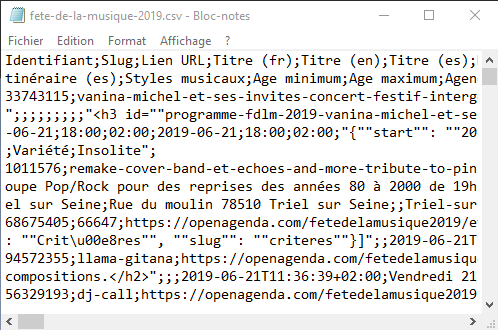
\includegraphics[height=4cm]{images/fetecsv.png} \qquad 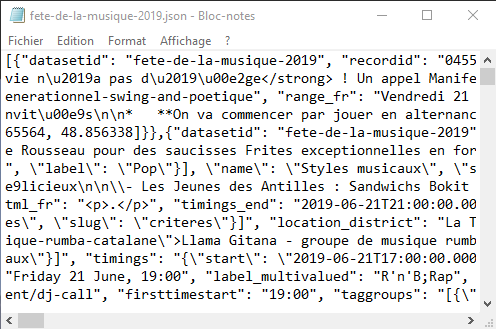
\includegraphics[height=4cm]{images/fetejson.png}\par}
	
	mais difficilement pour un humain, il y a un peu de travail !

Il existe cependant des outils pour nous aider (tableur : CSV, et navigateur web : JSON) :
	
	{\centering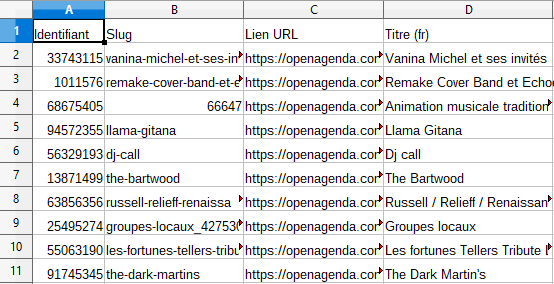
\includegraphics[height=3.5cm]{images/fetecsv2.png} \qquad 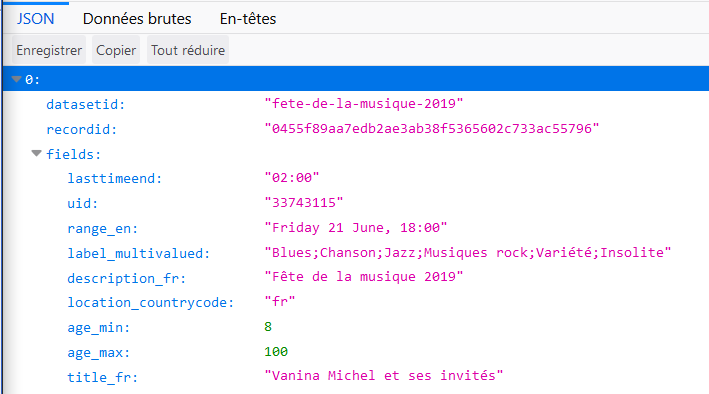
\includegraphics[height=3.5cm]{images/fetejson2.png}\par}

Si on regarde la première ligne du JSON : 

\texttt{[\{"datasetid": "fete-de-la-musique-2019", "recordid": "0455f89aa7edb2ae3}$\cdots$

on peut reconnaitre les formatage de listes et de dictionnaires Python. C'est ça qui permet de comprendre ce format. Si on regarde les deux premières lignes du CSV :

\texttt{Identifiant;Slug;Lien URL;Titre (fr);Titre (en);Titre (es);}$\cdots$

\texttt{33743115;vanina-michel-et-ses-invi}$\cdots$\texttt{ique;https://open}$\cdots$

La structure est beaucoup plus pauvre : 

\begin{itemize}
 \item Il n'y a qu'un séparateur (ici le << \texttt{;} >>).  
 \item La première ligne est réservée aux \emph{descripteurs}.
 \item Chacune des lignes suivantes correspond à une donnée définie par les valeurs correspondantes à ces descripteurs.
\end{itemize}

\medskip

Le but de cette partie est de traiter les données en tables donc au format CSV. Pour le format JSON, comme dit plus haut, on utilise un dictionnaire.

\section{Lecture/écriture d'un fichier texte}

Une table CSV est avant tout un fichier texte avec un certain format. 

Le langage Python dispose d'une fonction \pythoninline{open()} pour ouvrir un fichier en mode texte. 

Il dispose également d'une méthode \pythoninline{close()} pour le fermer :

\begin{multicols}{2}
\begin{minted}{python}
fichier = open('fichier.txt', 'w')
for i in range(1,4):
    fichier.write('Ligne '+srt(i)+'\n')
fichier.close()
\end{minted}

L'argument \pythoninline{'w'} pour << write >> ouvre (quitte à le créer) le fichier en écriture. Cet argument est \pythoninline{'r'} pour << read >> (ouverture en lecture) par défaut, et peut aussi être \pythoninline{'a'} pour << append >> (ouverture en ajout).
\end{multicols}

Pour éviter les problèmes de non-fermeture de fichier ouvert (si par exemple l'exécution du programme s'interrompt avant) on utilise le mot clé \pythoninline{with} qui gère le problème :

\begin{minted}{python}
with open('fichier.txt') as fichier :
    print(fichier.read())
\end{minted}

\begin{itemize}
	\item \pythoninline{fichier.read()} revoit une chaine de caractère contenant le fichier entier.
	\item \pythoninline{fichier.readlines()} aurait séparé chaque ligne dans une liste.
	
	\item On peut aussi itérer sur le fichier pour ne charger qu'une ligne en mémoire à la fois :

\begin{minted}{python}
with open('grosfichier.txt') as fichier :
    for ligne in fichier :
        print(ligne)
\end{minted}
\end{itemize}


Supposons disposer du fichier \texttt{notes.txt} contenant les trois lignes ci-dessous.

\begin{multicols}{2}

\vspace{-2ex}
\begin{minted}{text}
Nom;DS1;DS2;DS3;DS4;DS5
Bob;10;12;5;14;13 
Rick;12;10;ABS;12;11
\end{minted}

Si on perçoit les données comme un tableau à deux dimensions, on peut les extraire comme présenté ci-contre.

\pythoninline{ligne.rstrip('\r\n')} permet de nettoyer les fins de lignes et \pythoninline{ligne.split(';')} permet de créer une liste en séparant la chaîne au niveau des \pythoninline{';'}.

\begin{minted}{python}
# Extraction
notes = []
with open('notes.txt') as fnotes :
    for ligne in fnotes :
        ligne = ligne.rstrip('\r\n')
        notes.append(ligne.split(';'))

# Génération de l'index
index = {}
for (i, idx) in enumerate(notes[0]) :
    index[idx] = i
del(notes[0])
\end{minted}

\end{multicols}

La première ligne contenait les index. On répertorie leurs indices dans le dictionnaire \pythoninline{index} ( \pythoninline|= {'Nom' : 0, 'DS1' : 1,|...) et on la supprime du tableau de données \pythoninline{del(notes[0])}.

A présent la note de Bob au DS3 est \pythoninline{notes[0][index['DS3']]}.

\section{Importer une table CSV}

Les séparateurs \pythoninline{';'} et \pythoninline{'\r\n'} ne sont pas les seuls possibles. De plus, une des données à séparer pourrait être un texte comportant ces symboles... Une << bonne >> écriture d'extraction d'un fichier CSV est donc bien plus délicate à produire. Heureusement elle existe déjà dans la bibliothèque du même nom.

\medskip

Avec notre fichier \texttt{notes.txt}, cela donne :

\begin{minted}{python}
# Extraction
import csv

notes = []
with open('notes.csv') as fnotes:
    csvnotes = csv.reader(fnotes, delimiter=';')
    for ligne in csvnotes:
        notes.append(ligne)
\end{minted}

Les traitements comme  \pythoninline{ligne.replace('\n','')} ou
\pythoninline{ligne.split(';')} sont tous contenues dans \pythoninline{csv.reader()} et le rendu correspond aux listes attendues. 

\medskip


On peut avoir besoin de préciser l'encodage du texte en argument de la fonction \pythoninline{open()}. Pour le fichier \texttt{fete-de-la-musique-2019.csv} donné en exemple au début on pourra écrire :
\pythoninline{open('fete-de-la-musique-2019.csv', encoding='utf8')}

\medskip

{\bfseries Pour aller plus loin :}
Avec un fichier JSON, on peut utiliser la bibliothèque du même nom, et on obtient une liste de dictionnaires avec :

\vspace{-2ex}
\begin{minted}{python3}
import json

with open('fete-de-la-musique-2019.json', encoding='utf8') as ffete:
    fete = json.loads(ffete.read())
\end{minted}

\chapter{Manipulation de tables}

Il existe des modules pour le traitement de données issues de tables, comme \pythoninline{pandas}. Le parti pris pour la suite est de ne pas les utiliser. On considèrera donc les << tables >> de données comme étant des listes de listes ou de p-uplets Python  (on peut inclure les dictionnaires, si l'ordre n'a pas d'importance). 

L'exemple utilisé vient du fichier \texttt{fete-de-la-musique-2019.csv}, téléchargeable sur :

\href{https://www.data.gouv.fr/fr/datasets/r/49234ba7-00cd-401a-bb7c-70b81806b3eb}{https://www.data.gouv.fr/fr/datasets/fete-de-la-musique-2019/}

Et on suppose avoir fait l'indexation suivante :

\vspace{-2ex}
\begin{minted}{python}
import csv

table = []
with open('fete-de-la-musique-2019.csv', encoding='utf8') as ffete:
    csvfete = csv.reader(ffete, delimiter=';')
    for ligne in csvfete:
        table.append(ligne)

index = {}
for (i, idx) in enumerate(table[0]) :
    index[idx] = i
del(table[0])
\end{minted}

\section{Recherche dans une table}



En open data, on a souvent de gros fichiers, apportant beaucoup plus d'informations que ce que l'on cherche réellement. Il est donc important de pouvoir les sélectionner. Sur l'exemple de la fête de la musique, on peut vouloir ne s'intéresser qu'à une ville. On parcourt toutes les lignes de données et on récupère celles qui satisfont à ce critère : 

\begin{minted}{python}
laRocheSurYon = []
for ligne in table :
    if ligne[index['Ville']] == 'La Roche-sur-Yon' :
        laRocheSurYon.append(ligne)
\end{minted}

Il suffit de pouvoir exprimer ce critère avec des expression booléennes (en logique propositionnelle) : on emploie à loisir les \pythoninline{and},  \pythoninline{or},  \pythoninline{not}...

\medskip

On peut également vouloir filtrer certains index et donc supprimer certaines colonnes. Pour ce faire, on peut par exemple reconstruire une liste en sélectionnant ceux que l'on veut garder :

\begin{minted}{python}
simple = []
for ligne in laRocheSurYon :
    simple.append([ ligne[index['Titre (fr)']],
                    ligne[index['Nom du lieu']],
                    ligne[index['Première ouverture']] ])
\end{minted}

Une fois ces sélections effectuées (ou d'autres opérations), il peut arriver que certaines lignes soient identiques (par exemple, s'il ne reste plus que les valeurs de \texttt{Première ouverture} dans chaque ligne). On peut alors avoir besoin d'identifier/supprimer ces doublons.

On peut pour cela parcourir les données en recopiant celles qui ne l'ont pas déjà été :

\begin{minted}{python3}
unique = []
for ligne in simple:
    if ligne not in unique:
        unique.append(ligne)
\end{minted}

On peut améliorer ce code si la table était triée (les valeurs identiques seraient alors côte à côte.)

%%%%%%%%%%%%%%%%
%%%%%%|  |%%%%%%
%%%%%%|  |%%%%%%
%%%%%%|  |%%%%%%
%%%%\      /%%%%
%%%%%\    /%%%%%
%%%%%%\  /%%%%%%
%%%%%%%\/%%%%%%%
%%%%%%%%%%%%%%%%

{\color{rouge}\bfseries Tests de cohérence ?}

\section{Tri d'une table}

Des algorithmes de tri sont expliqués dans la partie algorithmique et peuvent bien sûr être appliqués. Pour ne pas surcharger, on propose ici d'utiliser la méthode \pythoninline{sort()} qui s'applique à une liste pour la trier selon une clé. Cette clé est une fonction qui prend en paramètre l'élément à trier et renvoie la valeur de cet élément dans ce tri :

\begin{minted}{python}
# On va trier selon la colonne d'indice 2
def valeurPourTrier(ligne):
    return ligne[2]

simple.sort(key = valeurPourTrier)
\end{minted}

On peut trier selon plusieurs critères, en faisant renvoyer un p-uplet comme clé.

On obtient un ordre total selon toutes les colonnes dans l'ordre si on ne précise pas de clé.
(L'amélioration de la suppression de doublon est alors possible...)

%
%Si hachable
%
%liste = [7, 8, 9, 5, 1, 7, 9, 5, 6, 2, 5, 3, 1, 4, 3, 2, 1]
%dictemp = {}
%newlist = [dictemp.setdefault(e,e) for e in liste if e not in dictemp]

\section{Fusion de tables}

On suppose disposer de deux tables comportant un champ en commun. Leur fusion consiste à les réunir en une seule table regroupant toutes les informations.

Prenons un exemple simple de deux tables déjà chargées et filtrées :

\begin{multicols}{2}

\begin{minted}[firstnumber=1]{python3}
index1 = ['Prénom', 'age']
table1 = [['Pierre', 12],
          ['Paulette', 14],
          ['Jack', 13]]
\end{minted}

\begin{minted}[firstnumber=5]{python3}
index2 = ['nom', 'Prénom']
table2 = [['Dupond','Pierre'],
          ['Pagnol','Pauline'],
          ['Potter','Jack']]
\end{minted}
\end{multicols}

Le champ commun est \pythoninline{'Prénom'}.

Un premier algorithme pour répondre à cette demande : 

On prépare la fusion en créant les champs nécessaires à partir d'une de table,

\begin{minted}[firstnumber=10]{python3}
index = [*index2, index1[1]]
fusion = []
for i in range(len(table2)):
    fusion.append([*table2[i],-1])
\end{minted}

 puis on parcourt l'autre table en cherchant pour chaque enregistrement s'il y en a un qui correspond pour les fusionner.
 
\begin{minted}[firstnumber=14]{python3}
for i in range(len(table1)):
    fusionOK = False
    for j in range(len(fusion)):
        if fusion[j][1] == table1[i][0]:
            fusion[j][2] = table1[i][1]
            fusionOK = True
    if not fusionOK :
        fusion.append(['',*table1[i]])
\end{minted}

\begin{itemize}
	\item S'il y avait eu deux prénoms identiques, la construction serait faussée.
	
	Il est important que le champ commun identifie clairement chaque enregistrement.
	
	Il est sinon possible de prendre plusieurs champs commun pour assurer cette unicité.
	\item On voit que la première partie complète le champ vide avec \pythoninline{-1} alors que dans la seconde, il est complété avec \pythoninline{''}. Il est important pour des traitements  ultérieurs de conserver le type de donnée associé à un champ. En proposant \pythoninline{-1} pour un âge qui devrait être positif et \pythoninline{''} pour un Nom qui devrait être au moins un caractère, on se place juste en dehors du domaine de valeurs du champ, pour spécifier qu'il n'est pas connu.
\end{itemize} 

\medskip

Si les deux tables étaient triées selon la valeur du champ commun, un algorithme de fusion beaucoup plus efficace existe : il parcourt les deux tables en même temps et ajoute à la fusion, à chaque étape, l'enregistrement le plus petit s'ils diffèrent entre les deux tables, ou leur fusion s'ils sont identiques.

\partie[IHM sur le Web]{Interactions entre l'homme et la machine sur le Web}
\chapter*{Programme officiel}

\section*{Programme officiel}

Lors de la navigation sur le Web, les internautes interagissent avec leur machine par le biais des pages Web.

L'Interface Homme-Machine (IHM) repose sur la gestion d'événements associés à des éléments graphiques munis de méthodes algorithmiques.

La compréhension du dialogue client-serveur déjà abordé en classe de seconde est consolidée, sur des exemples simples, en identifiant les requêtes du client, les calculs puis les réponses du serveur traitées par le client.

Il ne s'agit pas de décrire exhaustivement les différents éléments disponibles, ni de développer une expertise dans les langages qui permettent de mettre en œuvre le dialogue tels que PHP ou JavaScript.

{\centering\begin{tabular}{|L{3cm}|L{5.5cm}|L{6cm}|}\hline
\cellcolor{bo}\bfseries\textcolor{white}{Contenus}&
\cellcolor{bo}\bfseries\textcolor{white}{Capacités attendues}&
\cellcolor{bo}\bfseries\textcolor{white}{Commentaires}\\ \hline
Modalités de l'interaction entre l'homme et la machine

Événements
&
Identifier les différents composants graphiques permettant d'interagir avec une application Web.

Identifier les événements que les fonctions associées aux différents composants graphiques sont capables de traiter.
&
Il s'agit d'examiner le code HTML d'une page comprenant des composants graphiques et de distinguer ce qui relève de la description des composants graphiques en HTML de leur comportement (réaction aux événements) programmé par exemple en JavaScript.\\ \hline
Interaction avec l'utilisateur dans une page Web
&
Analyser et modifier les méthodes exécutées lors d'un clic sur un bouton d'une page Web.
&
\\ \hline
Interaction client-serveur.

Requêtes HTTP, réponses du serveur
&
Distinguer ce qui est exécuté sur le client ou sur le serveur et dans quel ordre.

Distinguer ce qui est mémorisé dans le client et retransmis au serveur.

Reconnaître quand et pourquoi la transmission est chiffrée.
&
Il s'agit de faire le lien avec ce qui a été vu en classe de seconde et d'expliquer comment on peut passer des paramètres à un site grâce au protocole HTTP.\\ \hline
Formulaire d'une page Web
&
Analyser le fonctionnement d'un formulaire simple.

Distinguer les transmissions de paramètres par les requêtes POST ou GET.
&
Discuter les deux types de requêtes selon le type des valeurs à transmettre et/ou leur confidentialité.\\ \hline
\end{tabular}\par}


\chapter{Les langages : HTML, CSS et JavaScript}

\section{Balises HTML}

\Cours{{\bfseries HTML} : HyperText Markup Language

C'est un langage de description de page web.

Un fichier HTML est un fichier texte, qui utilise des \emph{balises} pour définir la structure et le contenu d'une page Web (indépendamment de la façon de l'afficher).
}

Tout fichier HTML en français, devrait contenir au moins les dix lignes proposées ci-dessous.

\begin{multicols}{2}
Les éléments commençant et terminant par les chevrons \mintinline{html}{<} et \mintinline{html}{>} sont des \emph{balises}.

\begin{itemize}
	\item \mintinline{html}{<balise>} est une balise ouvrante,
	\item \mintinline{html}{</balise>} une balise fermante et
	\item \mintinline{html}{<balise />} une balise auto-fermante.
\end{itemize}

Toute balise ouverte doit être fermée.

Pour afficher les caractères < et > on utilise les entités : \mintinline{html}{&lt;} et \mintinline{html}{&gt;}.

\begin{minted}{HTML}
<!DOCTYPE html>
<html lang="fr">
  <head>
    <meta charset="UTF-8" />
    <title><!-- Un titre --></title>
  </head>
  <body>
    <!-- Du contenu -->
  </body>
</html>
\end{minted}
\end{multicols}

Quelques balises << indispensables >> :

\begin{multicols}{2}
\begin{tabular}{|ll|}
\hline
\multicolumn{2}{|c|}{Structurer le contenu}\\
\hline
\mintinline{html}{<h1>} & Titre principal \\
\mintinline{html}{<h2>} & Titre secondaire \\
\multicolumn{1}{|c}{\vdots} & \multicolumn{1}{c|}{\vdots} \\
\mintinline{html}{<h6>} & Plus petit sous-titre\\
\mintinline{html}{<p>}  & Paragraphe\\
\mintinline{html}{<br />} & Retour à la ligne\\
\hline
\end{tabular}


\begin{minted}[breaklines]{HTML}
<h1>Langage HTML</h1>

<h2>Les balises</h2>

<p>Ce sont les éléments commençant par
  &lt; et terminant par &gt;.<br />
  Exemple : &lt;br /&gt;</p>
\end{minted}
\end{multicols}

Les balises \mintinline{html}{<p>} et \mintinline{html}{<h1>}, ... sont de type \emph{block} : leur contenu prend toute la largeur disponible sur la page. Elles provoquent donc automatiquement un passage à la ligne. La balise générique de ce type est : \mintinline{html}{<div>}

\medskip

\begin{multicols}{2}
\begin{tabular}{|ll|}
\hline
\multicolumn{2}{|c|}{Faire des liens}\\
\hline
\mintinline{html}{<a>} & Lien hypertexte\\
\mintinline{html}{<img />} & Inclure une image \\
\hline
\end{tabular}


\begin{minted}[breaklines]{HTML}
<p>Cliquez l'image ci-dessous pour 
  aller sur mon site.<br />
  <a href="www.monsite.fr">
    <img src="../images/logo.png" />
  </a></p>
\end{minted}
\end{multicols}

Les balises \mintinline{html}{<a>} et \mintinline{html}{<img />}, ... sont de type \emph{inline} : leur contenu prend seulement la place dont il a besoin (pas de passage à la ligne). La balise générique de ce type est : \mintinline{html}{<span>}

\medskip

\begin{multicols}{2}
\begin{tabular}{|ll|}
\hline
\multicolumn{2}{|c|}{Faire une liste}\\
\hline
\mintinline{html}{<ul>} & Liste non numérotée\\
\mintinline{html}{<ol>} & Liste numérotée\\
\mintinline{html}{<li>} & Élément d'une liste\\
\hline
\end{tabular}


\begin{minted}{HTML}
<ul>
  <li> les balises <em>block</em></li>
  <li> les balises <em>inline</em></li>
</ul>
\end{minted}
\end{multicols}

La  balise \mintinline{html}{<em>} permet de mettre du texte en valeur (emphase). Il existe beaucoup d'autres balises dont on trouve facilement des listes et descriptions par exemple sur \href{https://www.w3schools.com/}{www.w3schools.com/}.

\section{Éléments de CSS}

\Cours{{\bfseries CSS} : Cascading Style Sheets

Un fichier CSS, appelé souvent << feuille de style >> est un fichier texte permettant de décrire la manière d'afficher ce qui est défini dans une page HTML.
}

Pour lier la feuille de style \texttt{style.css}, on inclut un lien dans l'entête de la page :

\begin{minted}{HTML}
<head>
  <!-- entête -->
  <link rel="stylesheet" type="text/css" href="chemin/style.css"/>
</head>
\end{minted}



\begin{multicols}{2}

La feuille de style permet alors de décrire l'affichage de chaque balise.

Par exemple on peut préciser la couleur d'un élément par un nom (dans une liste prédéfinie), par ses composantes \texttt{rgb} ou par son code hexadécimal.

\begin{minted}{CSS}
/* ---- généralités --- */
body {
  background-color : AliceBlue;
  color : rgb(128,128,255);
  border-color : #A1BBFF;
  border-style : solid;
}
\end{minted}
\end{multicols}

\medskip

Pour associer un style particulier à une seule balise du fichier HTML, on associe à cette balise un identifiant unique par le sélecteur \mintinline{html}{id} :

\begin{multicols}{2}
\begin{minted}{HTML}
<p id="particulier">Ce paragraphe 
  est traité de manière très 
  particulière.</p>
  
<p>Celui-ci ne change pas </p>

\end{minted}

\begin{minted}{CSS}
/* ---- cas particulier --- */
#particulier {
  text-align : center;
  font-size : 1.5vw; /* ou px ou em*/
}
\end{minted}
\end{multicols}

Pour associer un style particulier à plusieurs balises (éventuellement différentes) du fichier HTML, on associe à ces balises une classe commune par le sélecteur \mintinline{html}{class} :

\begin{multicols}{2}
\begin{minted}{HTML}
<h2 class="important"> Ce titre est 
important.</h2>
<p> Voila pourquoi </p>
<p class="important">Ce paragraphe 
  est important.</p>
\end{minted}
\begin{minted}{CSS}
/* ---- classe --- */
.important {
  text-decoration : underline;
  font-weight : bold;
}
\end{minted}

\end{multicols}

On peut préciser le style d'une balise selon son état. En particulier pour les liens :

\begin{multicols}{2}
\begin{minted}{HTML}
Pour la définition, voir le
<a href="mapage.html#chapitre1">
chapitre 1</a>.
\end{minted}

\begin{minted}{CSS}
/* ---- états --- */
a:link { color: red; }
a:visited { color: green; }
a:hover { color: hotpink; }
a:active { color: blue; }
\end{minted}

\end{multicols}

L'état \mintinline{html}{:hover}, en particulier, est utilisable pour les autres balises. 

\section{Notions de JavaScript}

\Cours{{\bfseries JavaScript}

C'est un langage de programmation, interprété par les navigateurs web.}

\mintinline{HTML}{<script>/* instructions */</script>} permet d'inclure des instructions JavaScript dans un document html. Mais on privilégie l'inclusion de fichiers : \mintinline{HTML}{<script src="script.js"></script>} pour garder la lisibilité de structure HTML. On peut, en sortie,  écrire dans 
\begin{itemize}
	\item la console du navigateur avec la fonction \mintinline{js}{console.log()} ;
	\item le document en train de s'afficher avec la fonction \mintinline{js}{document.write()} ;
	\item une fenêtre d'alerte avec la fonction \mintinline{js}{window.alert()} ;
	\item un élément de la page déjà affiché par son attribut \mintinline{js}{innerHTML}.
\end{itemize} 

\begin{multicols}{2}

\begin{minted}{HTML}
<!DOCTYPE html>
<html lang="fr">
  <head>
    <meta charset="UTF-8" />
    <title>Tests de sorties</title>
  </head>
  <body>
    <p>Paragraphe 1</p>
    <p id="fin">Paragraphe 2</p>
    <script src="script.js"></script>
  </body>
</html>
\end{minted}

Les instructions JavaScript, comme le contenu HTML, est interprété dans l'ordre des lignes.

\begin{minted}{js}
/* Fichier script.js*/
document.write("<strong>FIN</strong>");
var e = document.getElementById("FIN")
e.innerHTML = "Dernier paragraphe.";
console.log("Modification : OK.")
window.alert("Paragraphe 2 modifié !");
\end{minted}

\noindent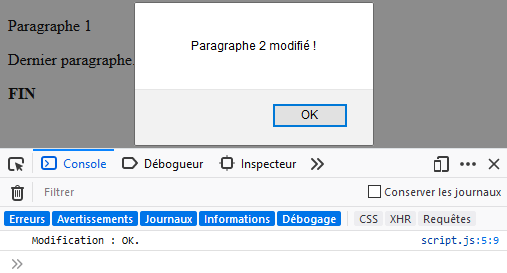
\includegraphics[width=\linewidth]{images/jslog.png}

\end{multicols}

Une fois un élément de la page HTML portant un identifiant récupéré par la fonction \mintinline{JS}{document.getElementById()}, on peut :

\begin{itemize}
	\item modifier ses attributs : \mintinline{JS}{e.setAttribute("attribut", "valeur");},
	\item supprimer ses attributs : \mintinline{JS}{e.removeAttribute("attribut");},
	\item agir sur sa classe (donc son style) : \mintinline{JS}{e.className = 'classe';}.
\end{itemize}

Et comme c'est un langage de programmation, on a les structures habituelles :

\begin{multicols}{3}\centering
Variables

\vspace{-2ex}
\begin{minted}[fontsize=\footnotesize]{js}
var x, y;
x = 7;
y = 7 ** 2;
\end{minted}

Appels de fonction

\vspace{-2ex}
\begin{minted}[fontsize=\footnotesize]{js}
function double(x) {
  return 2 * x;
}
console.log(double(7));
\end{minted}

Boucles bornées

\vspace{-2ex}
\begin{minted}[fontsize=\footnotesize]{js}
for (var i=0; i<9; i++) {
  console.log(i);
}
\end{minted}

Boucles non bornées

\vspace{-2ex}
\begin{minted}[fontsize=\footnotesize]{js}
var n = 0;
while (n < 3) {
  n++; console.log(n);
}
\end{minted}

Conditionnelles

\vspace{-2ex}
\begin{minted}[fontsize=\footnotesize]{js}
if (x < y) {
  console.log("ok");
} else {
  console.log("!!");
}
\end{minted}

(Chaque instruction étant terminée par un point-virgule.)
\end{multicols}

\section{Réaction aux événements}

\Cours{{\bfseries Événement}

Un événement est un changement d'état de l'environnement. Il peut être créé par l'utilisateur (avec le clavier, la souris...), par le document lui-même (fin de chargement d'une image, ou de la page...) ou encore par l'exécution d'un code JavaScript.}

\Cours{{\bfseries Gestionnaire d'événements}

Un événement une fois créé va se propager aux différents niveaux de définition de la page (document, html, body, jusqu'à l'élément cible et retour). Le rôle d'un gestionnaire d'événement est de l'intercepter et de réagir (souvent par un appel à une fonction JavaScript).}

Un gestionnaire d'événement peut être directement placé dans une balise HTML :

\vspace{-2ex}
\begin{minted}{html}
<!-- Dans l'en-tête -->
<script src="script.js"></script>
<link rel="stylesheet" type="text/css" href="style.css"/>
<!-- Dans le corps -->
<spam onmouseover="rouge(event)" onmouseout="noir(event)">Survolez-moi</spam>
\end{minted}

\vspace{-2ex}
\begin{multicols}{2}
avec dans \texttt{style.css} :

\vspace{-2ex}
\begin{minted}{css}
.noir { 
  color : black; 
}
.rouge { 
  color : red; 
}
\end{minted}


et dans \texttt{script.js} :

\vspace{-2ex}
\begin{minted}{css}
function rouge(e) {
  e.target.className = 'rouge'
} 
function noir(e) {
  e.target.className = 'noir'
}
\end{minted}

\end{multicols}

Dans cet exemple, passer sur les mots \texttt{Survolez-moi} ou les quitter avec la souris génère un événement. Il est capté par \mintinline{JS}{onmouseover} ou \mintinline{JS}{onmouseout} qui le transmettent aux fonctions JavaScript qui agissent sur le style graphique de ces mots. On peut citer de plus :

\begin{itemize}
	\item \mintinline{JS}{onchange} : un élément a changé.
	\item \mintinline{JS}{onclick} :  l'utilisateur a cliqué sur un élément.
	\item \mintinline{JS}{onkeydown} :  l'utilisateur a appuyé sur une touche.
	\item \mintinline{JS}{onload} : la page a fini d'être chargée.
\end{itemize}

L'élément cliquable par excellence est le bouton :

\vspace{-2ex}
\begin{minted}{html}
<button type="button" onclick="alert(event.target.innerHTML)">GO !</button>
\end{minted}

\chapter{Client, serveur et protocole HTTP}

\section{Modèle client/serveur}

Pour présenter ce modèle, on se place dans un réseau et sous le protocole de communication TCP/IP (voir partie Architectures matérielles). On ne considère que deux ordinateurs en train de communiquer.

\Cours{{\bfseries Modèle client/serveur}
\begin{multicols}{2}
C'est un modèle de communication dissymétrique entre deux ordinateurs sur un réseau.

\begin{itemize}
	\item Le client envoie une requête au serveur.
	\item Le serveur répond au client.
\end{itemize}

\begin{tikzpicture}
\node[](O){\ordinateur};\node[below]at(O.south){\small Client};
\node[right=2cm](S)at(O.east){\serveur};\node[below]at(S.south){\small Serveur};
\draw[-latex]($(O.east)+(0,0.3cm)$)--($(S.west)+(0,0.3cm)$)node[midway, above]{\small requête};
\draw[-latex]($(S.west)-(0,0.3cm)$)--($(O.east)-(0,0.3cm)$)node[midway, below]{\small réponse};
\end{tikzpicture}
\end{multicols}}

Voici une proposition minimaliste d'un client et d'un serveur en Python.

\begin{minted}{python}
import socket

hote = "localhost"
port = 12800

connexion = socket.socket(socket.AF_INET, socket.SOCK_STREAM)
connexion.connect((hote, port))
print("Connexion établie avec le serveur sur le port",port)

msg_a_envoyer = input("> ").encode()
connexion.send(msg_a_envoyer)
msg_recu = connexion.recv(1024)
print(msg_recu.decode())

connexion.close()
\end{minted}
\begin{tikzpicture}[overlay, xshift = 15cm, yshift=6.5cm]
\node[](O){\ordinateur};\node[below]at(O.south){\small Client};
\end{tikzpicture}

\vspace{-3ex}
On utilise un socket pour spécifier, selon le protocole TCP/IP, l'adresse du serveur et son port de communication. Ici, le serveur test est sur le même ordinateur que le client (\mintinline{python}{"localhost"}) et utilise le port 12800.

On peut observer les trois actions principales d'un client.

\begin{enumerate}
	\item La connexion avec le serveur (lignes 7)
	\item L'échange de messages (lignes 11 et 12)
	\item La déconnexion du serveur (ligne 15)
\end{enumerate}

Les messages échangés sont du domaine des applications (plus haute couche du modèle). Cela concerne par exemple les pages html (protocoles http ou https), l'échange de fichiers (protocole ftp) ou de mails (protocole smtp)...

\medskip

La requête (message envoyé au serveur) peut contenir des informations que le serveur traitera pour envoyer une réponse adaptée et personnelle à l'utilisateur (on parle de site dynamique, à opposer aux sites statiques qui ont un contenu indépendant de l'utilisateur). Ce traitement se fait à l'aide de programmation (avec différents langages : php ou python ou ...).

La réponse peut également contenir des éléments dynamiques pour l'utilisateur (en JavaScript par exemple).

\begin{minted}{python}
import socket

hote = ''
port = 12800

serveur = socket.socket(socket.AF_INET, socket.SOCK_STREAM)
serveur.bind((hote, port))
serveur.listen(5)
print("Le serveur écoute sur le port",port)

client, infos = serveur.accept()

msg_recu = client.recv(1024)
print(msg_recu.decode())
client.send(b"5 / 5")

client.close()
serveur.close()
\end{minted}
\begin{tikzpicture}[overlay, xshift = 15cm, yshift=7.5cm]
\node[](O){\serveur};\node[below]at(O.south){\small Serveur};
\end{tikzpicture}

\vspace{-2ex}
On peut observer les quatre actions principales d'un serveur.

\begin{enumerate}
	\item L'attente d'une connexion avec le client (lignes 8)
	\item La connexion avec un client (ligne 11)
	\item L'échange de messages (lignes 13 et 15)
	\item La déconnexion du client (ligne 17)
\end{enumerate}

Les réponses ne sont en général pas générées directement par le serveur. Il peut lui-même faire des requêtes à une base de données, récupérer des modèles et/ou demander à un autre programme de générer la vue à transmettre au client (le Modèle-Vue-Contrôleur : MVC).

\section{Protocole HTTP}

\Cours{{\bfseries HTTP} (HyperText Transfert Protocol)

C'est un protocole de la couche application (la plus haute sur modèle TCP/IP) permettant la demande et l'envoi de ressources. Il a été conçu pour la communication entre un navigateur web (client) et un serveur web.
}

Pour les premiers tests, on utilisera le serveur HTTP à l'adresse \href{http://httpbin.org/}{http://httpbin.org/} qui renvoie en écho les données utilisées dans la requête.

\subsection{Requête HTTP}

Une requête HTTP est de la forme :

\begin{minted}{text}
VERBE URI HTTP/X.X
En-têtes
Corps
\end{minted}

\begin{itemize}
	\item Le \mintinline{text}{VERBE} est le plus souvent \mintinline{text}{GET} pour \emph{obtenir} une ressource, ou \mintinline{text}{POST} pour \emph{envoyer}, par exemple, le contenu d'un formulaire.
	\item L'\mintinline{text}{URI} (Uniform Ressource Identifier) est l'URL (Uniform Ressource Locator) complété pour préciser la ressource visée à cette adresse.
	\item \mintinline{text}{HTTP/X.X} indique la version du protocole : \texttt{HTTP/1.1}
	\item \mintinline{text}{En-tête} (optionnel) permet de préciser la ressource et le comportement du client/serveur.
	
	Chaque ligne est composée d'un nom, de deux points \mintinline{text}{:} et de valeurs.

    Par exemple : \pythoninline{Accept-Language: fr,fr-FR;q=0.8,en-US;q=0.5,en;q=0.3}
	\item \mintinline{text}{Corps} contient des données précisant la demande de ressource. Cette partie est vide pour la méthode GET (qui peut tout de même préciser sa demande via l'URI).
\end{itemize}

En Python, on utilisera la bibliothèque \pythoninline{requests} (à installer).

Code minimal pour une requête GET, avec précisions au bout de l'URL :

\vspace{-2ex}
\begin{minted}{python}
import requests

ressource = requests.get('http://httpbin.org/get?test=True&valeur=2')
print(ressource.text)
\end{minted}

Affiche :

\vspace{-2ex}
\begin{minted}{text}
{
  "args": {
    "test": "True", 
    "valeur": "2"
  }, 
  "headers": {
    "Accept": "*/*", 
    "Accept-Encoding": "gzip, deflate", 
    "Host": "httpbin.org", 
    "User-Agent": "python-requests/2.22.0"
  }, 
  "origin": "xxx.xxx.xxx.xxx, xxx.xxx.xxx.xxx", 
  "url": "https://httpbin.org/get?test=True&valeur=2"
}
\end{minted}

On peut observer quelques éléments d'en-tête et que les précisions en bout d'URL ont bien été captées.

\medskip

Code minimal pour une requête POST, avec envoi de données encodées comme si elles venaient d'un formulaire HTML :

\vspace{-2ex}
\begin{minted}{python}
import requests

donnees = {'clef1': 'valeur1', 'clef2': 'valeur2'}
ressource = requests.post('http://httpbin.org/post', data = donnees)
print(ressource.text)
\end{minted}

Les données ont bien été transmises comme venant d'un formulaire :


\vspace{-2ex}
\begin{minted}{text}
{
  "args": {}, 
  "data": "", 
  "files": {}, 
  "form": {
    "test": "True", 
    "valeur": "2"
  }, 
  ...
\end{minted}

Si ces données ne sont pas trop importantes, elles peuvent être envoyées par la méthode GET mais seront visibles dans l'URI. Celles transmises par la méthode POST ne le sont pas, mais restent transmises en clair, dans le corps de la requête. Si on souhaite une transmission sécurisée, il faudra en plus utiliser un système de chiffrement.

\medskip

{\bfseries Pour aller plus loin :} D'autres façons de transmettre les données sont possibles.

Par exemple en JSON :

\vspace{-2ex}
\begin{minted}{python}
import requests
import json

donnees = {'test': True, 'valeur': 2}
donneesJSON = json.dumps(donnees)
ressource = requests.post('http://httpbin.org/post', data = donneesJSON)
\end{minted}

Ou sinon directement en chaîne de caractères :

\vspace{-2ex}
\begin{minted}{python}
import requests

donnees = "Ma structure"
ressource = requests.post('http://httpbin.org/post', data = donnees)
\end{minted}



\subsection{Réponse HTTP}

Une réponse HTTP a la même forme qu'une requête sauf pour la première ligne :

\begin{minted}{text}
HTTP/X.X CODE MESSAGE
En-têtes
Corps
\end{minted}

\begin{itemize}
	\item \pythoninline{CODE} et  \pythoninline{MESSAGE} indiquent le statut de la communication.
	
	Exemples : \mintinline{text}{200 OK} ou le fameux \mintinline{text}{404 Not Found}. Voir \href{https://httpstatuses.com/}.{https://httpstatuses.com/}
	
	On peut obtenir le CODE d'une réponse par : \pythoninline{ressource.status_code}.
	\item On peut obtenir l'\mintinline{text}{en-tête} par : \pythoninline{ressource.headers} (donne un dictionnaire).
	\item On peut obtenir le \mintinline{text}{corps} au format texte par : \pythoninline{ressource.text}.
	      
	      En précisant \emph{avant} l'encodage si besoin : \pythoninline{ressource.encoding = 'utf-8'}.
	
	\item On peut obtenir le corps au format JSON par : \pythoninline{ressource.json}.
\end{itemize}

\chapter{Formulaires}

Les formulaires permettent facilement de faire des requêtes directement depuis une page HTML. Pour y répondre, un autre langage (Python, PHP, JavaScript, ...) sera nécessaire.

\section{Construction et envoi d'une requête}

Un formulaire HTML est délimité par la balise \mintinline{html}{<form>} en précisant deux attributs :

\begin{itemize}
	\item \mintinline{html}{method} égal à \mintinline{html}{"get"} ou \mintinline{html}{"post"} selon le type de requête.
	\item \mintinline{html}{action} égal à l'URL de la page ou du programme qui devra traiter cette requête.
\end{itemize}

Le bouton d'envoi peut s'écrire : \mintinline{html}{<input type="submit" value="Envoyer" />}

Un formulaire minimal provoquant une requête GET pourrait être :

\vspace{-2ex}
\begin{minted}{html}
<!doctype html>
<html lang="fr">
    <head>
        <meta charset="utf-8">
        <title>Le formulaire GET</title>
    </head>
    <body>
        <form action="http://httpbin.org/get" method="get">
            <input type="submit" value="GET !" />
        </form>
    </body>
</html>
\end{minted}

\mintinline{html}{<a href="http://httpbin.org/get">GET !</a>} aurait tout aussi bien fait l'affaire !

Un formulaire n'a effectivement de sens que si l'utilisateur peut sélectionner ses entrées.

C'est encore la balise \mintinline{html}{<input />} qui joue ce rôle.

\mintinline{html}{<input type="text" name="nom" />} par exemple permet à l'utilisateur d'entrer une chaine de caractères, qui sera envoyé sous le nom \pythoninline{"nom"}.

Pour une interface graphique claire, on peut lier un tel champ d'entrée (s'il est identifié par un \mintinline{html}{id}) avec une description en utilisant la balise \mintinline{html}{<label>} (en donnant à son attribut \mintinline{html}{for} l'identifiant en question) :

\vspace{-2ex}
\begin{minted}[firstline=8,lastline=12]{html}
<!doctype html>
<html lang="fr">
    <head>
        <meta charset="utf-8">
        <title>Le formulaire GET</title>
    </head>
    <body>
        <form action="http://httpbin.org/get" method="get">
            <label for="nom">Nom</label> :
            <input type="text" name="nom" id="nom" />
            <input type="submit" value="GET !" />
        </form>
    </body>
</html>
\end{minted}

L'équivalent avec la méthode POST :

\vspace{-2ex}
\begin{minted}[firstline=8,lastline=12]{html}
<!doctype html>
<html lang="fr">
    <head>
        <meta charset="utf-8">
        <title>Le formulaire GET</title>
    </head>
    <body>
        <form action="http://httpbin.org/post" method="post">
            <label for="nom">Nom</label> :
            <input type="text" name="nom" id="nom" />
            <input type="submit" value="POST !" />
        </form>
    </body>
</html>
\end{minted}

On peut préciser la taille du champ avec l'attribut \mintinline{html}{size}, le nombre maximum de caractères à saisir avec  \mintinline{html}{maxlength}, une valeur prédéfinie par  \mintinline{html}{value}ou une simple indication de contenu par  \mintinline{html}{placeholder}. On peut rendre un champ obligatoire avec l'attribut \mintinline{html}{required}, non modifiable avec \mintinline{html}{readonly}...

Valeurs possibles de l'attribut \mintinline{html}{type} :

\begin{itemize}
	\item \mintinline{html}{<input type="password" name="psw" />} (La valeur n'apparait pas.)
	\item \mintinline{html}{<input type="reset" />} (Le formulaire est réinitialisé.)
	\item \mintinline{html}{<input type="radio" name="genre" value="homme" checked /> Homme<br />}.
	
	      \mintinline{html}{<input type="radio" name="genre" value="femme" /> Femme<br />}.
	      
	      (Un seul peut être sélectionné à la fois.)
	\item \mintinline{html}{<input type="checkbox" name="finrepas" value="fromage" /> Fromage<br />}.
	
	      \mintinline{html}{<input type="checkbox" name="finrepas" value="dessert" checked /> Dessert<br />}.
	      
	      (Sélection libre.)
	\item \mintinline{html}{ <input type="button" onclick="alert('Bonjour !')" value="Bonjour !"> } 
	\item et des types << text enrichi >> (ramenés à text simple si non pris en charge par le navigateur) : \mintinline{html}{"color"}, \mintinline{html}{"date"}, \mintinline{html}{"datetime-local"}, \mintinline{html}{"email"}, \mintinline{html}{"month"}, \mintinline{html}{"number"}, \mintinline{html}{"range"}, \mintinline{html}{"search"}, \mintinline{html}{"tel"}, \mintinline{html}{"time"}, \mintinline{html}{"url"} ou \mintinline{html}{"week"}

\end{itemize}

\section{Réponse ?}

Pour répondre, on sous-entend être du côté serveur. Déjà, il faut arriver à capter la demande. Le langage dédié sur le web est le PHP : 

\begin{multicols}{2}
\begin{minted}{php}
<?php
$nom = htmlspecialchars($_GET["nom"]);
?>
\end{minted}

\begin{minted}{php}
<?php
$nom = htmlspecialchars($_POST["nom"]);
?>
\end{minted}
\end{multicols}

Mais ce langage n'est pas un objectif de première.

On peut proposer un serveur minimal en Python (navigateur en \texttt{Localhost:8765/valeur}) :

\begin{minted}{python3}
from http.server import BaseHTTPRequestHandler, HTTPServer

class Gestionnaire(BaseHTTPRequestHandler):

    def do_GET(self):
        html = """<!doctype html><html>
<head><meta charset="utf-8"><title>Serveur minimal GET</title></head>
<body><p>""" + str(self.path) + "</p></body></html>"
        self.send_response(200)
        self.send_header("Content-Type", "text/html; charset=utf-8")
        self.end_headers()
        self.wfile.write(html.encode("utf-8"))

if __name__ == "__main__":
    print("Lancement du serveur minimal")
    httpd = HTTPServer(('', 8765), Gestionnaire)
    httpd.serve_forever()
    httpd.server_close()
\end{minted}

% Pour do_POST(self)
% length = int(self.headers['Content-Length'])
% data = self.rfile.read(length).decode('utf-8')

mais là encore, on dépasse les attendus de première !

\medskip

On ne s'étendra donc pas sur le sujet.

\partie[Architectures matérielles et SE]{Architectures matérielles et systèmes d'exploitation}
\chapter*{Programme officiel}

\section*{Programme officiel}

Exprimer un algorithme dans un langage de programmation a pour but de le rendre exécutable par une machine dans un contexte donné. La découverte de l'architecture des machines et de leur système d'exploitation constitue une étape importante.

Les circuits électroniques sont au cœur de toutes les machines informatiques. Les réseaux permettent de transmettre l'information entre machines. Les systèmes d'exploitation gèrent et optimisent l'ensemble des fonctions de la machine, de l'exécution des programmes aux entrées-sorties et à la gestion d'énergie.

On étudie aussi le rôle des capteurs et actionneurs dans les entrées-sorties clavier, interfaces graphiques et tactiles, dispositifs de mesure physique, commandes de machines, etc.

{\centering\begin{tabular}{|L{3cm}|L{5.5cm}|L{6cm}|}\hline
\cellcolor{bo}\bfseries\textcolor{white}{Contenus}&
\cellcolor{bo}\bfseries\textcolor{white}{Capacités attendues}&
\cellcolor{bo}\bfseries\textcolor{white}{Commentaires}\\ \hline
Modèle d'architecture séquentielle (von Neumann)
&
Distinguer les rôles et les caractéristiques des différents constituants d'une machine.

Dérouler l'exécution d'une séquence d'instructions simples du type langage machine.
&
La présentation se limite aux concepts généraux.

On distingue les architectures monoprocesseur et les architectures multiprocesseur.

Des activités débranchées sont proposées.

Les circuits combinatoires réalisent des fonctions booléennes.\\ \hline
Transmission de données dans un réseau

Protocoles de communication

Architecture d'un réseau

&
Mettre en évidence l'intérêt du découpage des données en paquets et de leur encapsulation.

Dérouler le fonctionnement d'un protocole simple de récupération de perte de paquets (bit alterné).

Simuler ou mettre en œuvre un réseau.
&
Le protocole peut être expliqué et simulé en mode débranché.

Le lien est fait avec ce qui a été vu en classe de seconde sur le protocole TCP/IP.

Le rôle des différents constituants du réseau local de l'établissement est présenté.\\ \hline
Systèmes d'exploitation
&
Identifier les fonctions d'un système d'exploitation.

Utiliser les commandes de base en ligne de commande.

Gérer les droits et permissions d'accès aux fichiers.
&
Les différences entre systèmes d'exploitation libres et propriétaires sont évoquées.

Les élèves utilisent un système d'exploitation libre.

Il ne s'agit pas d'une étude théorique des systèmes d'exploitation.\\ \hline
Périphériques d'entrée et de sortie

Interface Homme-Machine (IHM)
&
Identifier le rôle des capteurs et actionneurs.

Réaliser par programmation une IHM répondant à un cahier des charges donné.
&
Les activités peuvent être développées sur des objets connectés, des systèmes embarqués ou robots.\\ \hline
\end{tabular}\par}


\chapter{Modèle d'architecture}

\section{Qu'est-ce qu'un ordinateur ?}


\noindent\date{1945} Le mathématicien John von Neumann élabore la première description d'un ordinateur. On peut la simplifier ainsi :

\begin{center}\begin{tikzpicture}
\node[text width = 3cm, draw, align=center](A){\raisebox{-1ex}{\rule{0pt}{4ex}}Processeur};
\node[text width = 3cm, draw, align=center, xshift=2.5cm](B)at(A.east){\raisebox{-1ex}{\rule{0pt}{4ex}}Mémoire};
\node[text width = 3cm, draw, align=center, xshift=2.5cm](C)at(B.east){\raisebox{-1ex}{\rule{0pt}{4ex}}Entrées/Sorties};
\node[text width = 12cm, draw, align=center, yshift=-1cm, double arrow](D)at(B.south){Bus de communication};
\draw(A.south)--++($(D.north)-(B.south)$);
\draw(B.south)--++($(D.north)-(B.south)$);
\draw(C.south)--++($(D.north)-(B.south)$);
\end{tikzpicture}\end{center}

\Cours{{\bfseries Ordinateur}

Un ordinateur est une machine \emph{électronique} capable d'exécuter des \emph{instructions} effectuant des \emph{opérations} sur des \emph{nombres}.}

\subsection{Entrées/sorties}

\Cours{{\bfseries Entrées/sorties}

\begin{itemize}
    \item Un périphérique d'entrée permet de fournir des informations au système. 
    
    Exemples : Clavier, souris, scanner, micro, etc.
    \item Un périphérique de sortie permet de faire sortir des informations du système.
    
    Exemples : Écran, imprimante, haut-parleurs, etc.
    \item Un périphérique d'entrée/sortie permet l'échange d'informations dans les deux sens.
    
    Exemples : Clé USB, Carte son, carte réseau, etc.
\end{itemize}}

\subsection{Mémoires}

\Cours{{\bfseries Mémoire vie / Mémoire morte}

\begin{itemize}
    \item La mémoire vive ou temporaire est celle des barrettes de RAM (Random Access Memory), qui ne persiste pas hors tension.
    \item La mémoire morte ou persistante est celle du disque dur (Hard Drive), qui permet une mémorisation permanente.
\end{itemize}}

La mémoire vive est indispensable pour sa vitesse d'accès ($\approx 10$ns contre $\approx 5$ms pour la mémoire morte) et la mémoire morte est indispensable pour sa persistance.

De nos jours, les processeurs eux-mêmes sont dotés de leur propre petite mémoire vive, dite mémoire cache, pour augmenter les vitesses d'accès ($\approx 5$ns). Ils fonctionnent par ailleurs en manipulant de touts petits espaces mémoires appelés registres, encore plus rapides ($\approx 1$ns).



\subsection{Processeur}

\Cours{{\bfseries Processeur}

Le processeur est le composant électronique qui permet d'effectuer les calculs.
}

L'élément constitutif de base est le \emph{transistor}, sorte d'interrupteur, contrôlé, qui permet, ou non, de laisser passer le courant, donc aboutissant à deux états possibles : 0 ou 1. Le processeur ne travaille fondamentalement qu'avec \emph{deux chiffres}, donc avec des \emph{nombres binaires}.

\begin{center}\begin{tikzpicture}
\node(A){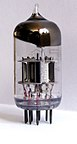
\includegraphics[scale=0.5]{images/tube.jpg}};
\node[yshift=-1.5cm]at(A){tube};
\node[xshift=3cm](B)at(A){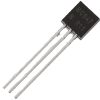
\includegraphics[scale=0.5]{images/transistor.png}};
\node[yshift=-1.5cm]at(B){transistor};
\node[xshift=3cm](C)at(B){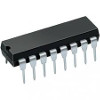
\includegraphics[scale=0.5]{images/ci.jpg}};
\node[yshift=-1.5cm]at(C){circuit itégré};
\end{tikzpicture}\end{center}

\noindent\date{1943} Le premier ordinateur, le Colossus était conçu à partir de tubes électroniques.

De nos jours, les transistors des processeurs ne font que quelques nanomètres et se comptent en milliards.
Combiner plusieurs transistors permet la création de \emph{circuits logiques}. Il en existe de deux types :

\begin{itemize}
	\item les circuits combinatoires, si les sorties ne sont fonction que des entrées.
	\item les circuits séquentiels, si les sorties dépendent également du temps et des états antérieurs.
\end{itemize}
\section{Circuits combinatoires}

\subsection{Porte non}
Le circuit combinatoire le plus simple celui qui permet de changer d'état :

\begin{itemize}
	\item Si l'entrée est $E=1$ alors la sortie est $S = 0$
	\item Si l'entrée est $E=0$ alors la sortie est $S = 1$
\end{itemize}

On identifie 0 à << faux >> et 1 à << vrai >> et ce circuit correspond alors à une négation : ce qui était vrai devient faux et ce qui était faux devient vrai. On appelle ce circuit une << porte non >> :


\begin{center}
\begin{multicols}{2}
Porte non

\begin{tikzpicture}
    \draw node[not port](not) {}; 
    \draw (not.out)--++(0.25,0)node[right]{$S$}; 
    \draw (not.in)--++(-0.25,0)node[left]{$E$};
\end{tikzpicture}

Table de vérité :

\begin{tabular}{c|c}
$E$ & $S$ \\
\hline
$0$ & $1$ \\
$1$ & $0$ \\
\end{tabular}
\end{multicols}
\end{center}

{\bfseries Pour aller plus loin : } ce circuit n'est composé que de deux transistors :

\ctikzset{tripoles/mos style/arrows}

nMOS \quad \begin{tikzpicture}[baseline=(G.base)]
\node[nmos](nmos){};
\node[left](G)at(nmos.G){$G$};
\node[above]at(nmos.D){$D$};
\node[below]at(nmos.S){$S$};
\end{tikzpicture}
\qquad équivalent à : \quad
\begin{tikzpicture}[baseline=(G.base)]
\draw[](0,0)node[above]{D}--++(0,-0.5cm)node[inner sep = 0,circle,draw,fill=black](I){\rule{3pt}{0pt}};
\draw(I)--++(-120:0.5cm);
\draw[](0,-1.5cm)node[below]{S}--++(0,0.5cm)node[inner sep = 0,circle,draw,fill=black]{\rule{3pt}{0pt}};
\node[left](G)at(-0.25cm,-0.75cm){$G=0$};
\node[right](G)at(0.25cm,-0.75cm){OFF};
\end{tikzpicture}
\qquad
\begin{tikzpicture}[baseline=(G.base)]
\draw[](0,0)node[above]{D}--++(0,-0.5cm)node[inner sep = 0,circle,draw,fill=black](I){\rule{3pt}{0pt}};
\draw(I)--++(-90:0.5cm);
\draw[](0,-1.5cm)node[below]{S}--++(0,0.5cm)node[inner sep = 0,circle,draw,fill=black]{\rule{3pt}{0pt}};
\node[left](G)at(-0.25cm,-0.75cm){$G=1$};
\node[right](G)at(0.25cm,-0.75cm){ON};
\end{tikzpicture}


pMOS \quad \begin{tikzpicture}[baseline=(G.base)]
\node[pmos,emptycircle](pmos){};
\node[left](G)at(pmos.G){$G$};
\node[below]at(pmos.D){$D$};
\node[above]at(pmos.S){$S$};
\end{tikzpicture}
\qquad équivalent à : \quad
\begin{tikzpicture}[baseline=(G.base)]
\draw[](0,0)node[above]{S}--++(0,-0.5cm)node[inner sep = 0,circle,draw,fill=black](I){\rule{3pt}{0pt}};
\draw(I)--++(-90:0.5cm);
\draw[](0,-1.5cm)node[below]{D}--++(0,0.5cm)node[inner sep = 0,circle,draw,fill=black]{\rule{3pt}{0pt}};
\node[left](G)at(-0.25cm,-0.75cm){$G=0$};
\node[right](G)at(0.25cm,-0.75cm){ON};
\end{tikzpicture}
\qquad
\begin{tikzpicture}[baseline=(G.base)]
\draw[](0,0)node[above]{S}--++(0,-0.5cm)node[inner sep = 0,circle,draw,fill=black](I){\rule{3pt}{0pt}};
\draw(I)--++(-120:0.5cm);
\draw[](0,-1.5cm)node[below]{D}--++(0,0.5cm)node[inner sep = 0,circle,draw,fill=black]{\rule{3pt}{0pt}};
\node[left](G)at(-0.25cm,-0.75cm){$G=1$};
\node[right](G)at(0.25cm,-0.75cm){OFF};
\end{tikzpicture}

\begin{tikzpicture}[baseline=(E.base)]
\node[pmos,emptycircle](pmos){};
\node[nmos, yshift=-1.5cm](nmos)at(pmos){};
\node[above]at(pmos.S){1 (alim)};
\node[below]at(nmos.S){0 (mass)};
\draw(pmos.G)--(nmos.G);
\draw($0.5*(pmos.G)+0.5*(nmos.G)$)--++(-0.25cm,0)node(E)[left]{$E$};
\draw($0.5*(pmos.D)+0.5*(nmos.D)$)--++(0.25cm,0)node[right]{$S$};
\end{tikzpicture}\qquad donne : \quad
\begin{tikzpicture}[baseline=(E.base)]
\draw[](0,0)node[above]{1}--++(0,-0.5cm)node[inner sep = 0,circle,draw,fill=black](I){\rule{3pt}{0pt}};
\draw(I)--++(-90:0.5cm)node[inner sep = 0,circle,draw,fill=black]{\rule{3pt}{0pt}}
     --++(0cm,-0.5cm)node[left=1cm](E){$E=0$}
     --++(0cm,-0.5cm)node[inner sep = 0,circle,draw,fill=black]{\rule{3pt}{0pt}}
     --++(-120:0.5cm);
\draw(0cm,-2.5cm)node[inner sep = 0,circle,draw,fill=black]{\rule{3pt}{0pt}}--++(0,-0.5cm)node[below]{0};
\draw(E.east)--++(0.25cm,0)|-++(0.25,0.75)node[inner sep = 0,circle,draw,fill=white](I){\rule{3pt}{0pt}};
\draw(E.east)++(0.25cm,0)|-++(0.25,-0.75);
\draw(E.east)++(1cm,0)--++(0.5cm,0)node[right]{$S=1$};
\end{tikzpicture}
\qquad
\begin{tikzpicture}[baseline=(E.base)]
\draw[](0,0)node[above]{1}--++(0,-0.5cm)node[inner sep = 0,circle,draw,fill=black](I){\rule{3pt}{0pt}};
\draw(I)--++(-120:0.5cm);
\draw(I)++(0,-0.5cm)node[inner sep = 0,circle,draw,fill=black]{\rule{3pt}{0pt}}
     --++(0cm,-0.5cm)node[left=1cm](E){$E=1$}
     --++(0cm,-0.5cm)node[inner sep = 0,circle,draw,fill=black]{\rule{3pt}{0pt}}
     --++(-90:0.5cm);
\draw(0cm,-2.5cm)node[inner sep = 0,circle,draw,fill=black]{\rule{3pt}{0pt}}--++(0,-0.5cm)node[below]{0};
\draw(E.east)--++(0.25cm,0)|-++(0.25,0.75)node[inner sep = 0,circle,draw,fill=white](I){\rule{3pt}{0pt}};
\draw(E.east)++(0.25cm,0)|-++(0.25,-0.75);
\draw(E.east)++(1cm,0)--++(0.5cm,0)node[right]{$S=0$};
\end{tikzpicture}


\subsection{Portes et / ou / ou exclusif}

Les portes logiques suivantes admettent deux entrées et une sortie.

\begin{center}
\begin{multicols}{3}
Porte et

\medskip

\begin{tikzpicture}
    \draw node[and port](and) {}; 
    \draw (and.out)--++(0.25,0)node[right]{$S$}; 
    \draw (and.in 1)--++(-0.25,0)node[left]{$E_1$};
    \draw (and.in 2)--++(-0.25,0)node[left]{$E_2$};
\end{tikzpicture}

\pythoninline{S = E1 & E2}

\medskip

\begin{tabular}{cc|c}
$E_1$ & $E_2$ & $S$ \\
\hline
$0$ & $0$ & $0$ \\
$0$ & $1$ & $0$\\
$1$ & $0$ & $0$ \\
$1$ & $1$ & $1$\\
\end{tabular}

\columnbreak
Porte ou

\medskip

\begin{tikzpicture}
    \draw node[or port](or) {}; 
    \draw (or.out)--++(0.25,0)node[right]{$S$}; 
    \draw (or.in 1)--++(-0.25,0)node[left]{$E_1$};
    \draw (or.in 2)--++(-0.25,0)node[left]{$E_2$};
\end{tikzpicture}

\pythoninline{S = E1 | E2}

\medskip

\begin{tabular}{cc|c}
$E_1$ & $E_2$ & $S$ \\
\hline
$0$ & $0$ & $0$ \\
$0$ & $1$ & $1$\\
$1$ & $0$ & $1$ \\
$1$ & $1$ & $1$\\
\end{tabular}

\columnbreak

Porte ou  exclusif

\medskip

\begin{tikzpicture}
    \draw node[xor port](xor) {}; 
    \draw (xor.out)--++(0.25,0)node[right]{$S$}; 
    \draw (xor.in 1)--++(-0.25,0)node[left]{$E_1$};
    \draw (xor.in 2)--++(-0.25,0)node[left]{$E_2$};
\end{tikzpicture}

\pythoninline{S = E1 ^ E2}
\medskip

\begin{tabular}{cc|c}
$E_1$ & $E_2$ & $S$ \\
\hline
$0$ & $0$ & $0$ \\
$0$ & $1$ & $1$\\
$1$ & $0$ & $1$ \\
$1$ & $1$ & $0$\\
\end{tabular}
\end{multicols}
\end{center}

Sur ce modèle, on pourrait dresser $2^4=16$ tables de vérité différentes (même si certaines n'ont pas d'intérêt : $S$ toujours à 0 ou toujours à 1...). Pour arriver à faire des additions (binaires), ces trois portes suffisent.

\subsection{Demi additionneur (half adder)}

Posons les additions à un bit :

\begin{center}
\begin{multicols}{4}
\begin{tabular}{ccc}
    &   & $0$ \\
$+$ &   & $0$ \\
\hline
    &   & $0$\\
\end{tabular}


\begin{tabular}{ccc}
    &   & $1$ \\
$+$ &   & $0$ \\
\hline
    &   & $1$\\
\end{tabular}


\begin{tabular}{ccc}
    &   & $0$ \\
$+$ &   & $1$ \\
\hline
    &   & $1$\\
\end{tabular}


\begin{tabular}{ccc}
    &   & $1$ \\
$+$ &   & $1$ \\
\hline
    &$1$& $0$\\
\end{tabular}
\end{multicols}
\end{center}

Il n'y a une retenue que si les deux bit sont à 1 ($\Rightarrow$ porte et)

Mise à part la retenue, le résultat est 1 seulement si un seul bit est 1 ($\Rightarrow$ porte ou exclusif)

\begin{center}
\begin{multicols}{3}
\begin{tikzpicture}
    \node[xor port](xor){}; 
    \draw (xor.out)--++(0.25,0)node[right]{$S$}; 
    \draw (xor.in 1)--++(-0.5,0)node[left]{$A$};
    \draw (xor.in 2)--++(-0.5,0)node[left]{$B$};
    \node[and port, yshift=-1.5cm](and)at(xor){}; 
    \draw (and.out)--++(0.25,0)node[right]{$R$}; 
    \draw (xor.in 2)node{$\bullet$}--(and.in 1);
    \draw (xor.in 1)++(-0.25cm,0)node{$\bullet$}|-(and.in 2);
\end{tikzpicture}

La somme :

\pythoninline{S = A ^ B}

\smallskip

La retenue :

\pythoninline{R = A & B}

\begin{tabular}{cc|c|c}
$A$ & $B$ & $R$ & $S$ \\
\hline
$0$ & $0$ & $0$ & $0$ \\
$0$ & $1$ & $0$ & $1$\\
$1$ & $0$ & $0$ & $1$ \\
$1$ & $1$ & $1$ & $0$\\
\end{tabular}
\end{multicols}
\end{center}

\subsection{Plein additionneur (full adder)}

Pour additionner deux entiers écrits en binaire, il est nécessaire de tenir compte des retenues à chaque addition de deux bits :

\begin{center}
\begin{tabular}{ccccc}
    & {\scriptsize$0$} & {\scriptsize$1$} & {\scriptsize$1$} &   \\
    & $1$ & $0$ & $1$ & $1$ \\
$+$ & $0$ & $0$ & $1$ & $1$ \\
\hline
    & $1$ & $1$ & $1$ & $0$\\
\end{tabular}
\end{center}

Notons $R_0$ la retenue dont il faut tenir compte. 

On peut compléter la table de vérité (ci-dessous).

Pour calculer $S$ on utilise de nouveau un demi additionneur pour ajouter $R_0$ ; et la retenue $R$ vaut 1 dès que l'un des deux demi additionneurs renvoie une retenue à 1. 
\begin{center}
\begin{multicols}{2}

\begin{tabular}{ccc|c|c}
$R_0$ & $A$ & $B$ & $R$ & $S$ \\
\hline
$0$ & $0$ & $0$ & $0$ & $0$ \\
$0$ & $0$ & $1$ & $0$ & $1$ \\
$0$ & $1$ & $0$ & $0$ & $1$ \\
$0$ & $1$ & $1$ & $1$ & $0$ \\
$1$ & $0$ & $0$ & $0$ & $1$ \\
$1$ & $0$ & $1$ & $1$ & $0$ \\
$1$ & $1$ & $0$ & $1$ & $0$ \\
$1$ & $1$ & $1$ & $1$ & $1$ \\
\end{tabular}

\medskip

\pythoninline{S = A ^ B ^ R0}

\pythoninline{R = (A & B) | (R0 & (A ^ B))}

~

\begin{tikzpicture}
    \node[xor port](xor1){}; 
    \node[and port, yshift=-1.5cm](and1)at(xor1){}; 
    \draw (xor1.in 2)node{$\bullet$}--(and1.in 1);
    \draw (xor1.in 1)++(-0.25cm,0)node{$\bullet$}|-(and1.in 2);
    \draw[dotted]($(xor1.in 1)+(-0.5cm,0.5cm)$)rectangle($(and1.in 2)+(1.5cm,-0.5cm)$);
    \node[xor port, xshift=2.75cm](xor2)at(xor1){};
    \node[and port, yshift=-1.5cm](and2)at(xor2){}; 
    \draw (xor.out)--++(0.25cm,0)|-(xor2.in 2)node{$\bullet$}--(and2.in 1);
    \draw (xor2.in 1)++(-0.25cm,0)node{$\bullet$}|-(and2.in 2);
    \draw[dotted]($(xor2.in 1)+(-0.5cm,0.5cm)$)rectangle($(and2.in 2)+(1.5cm,-0.5cm)$);
    \node[or port, rotate=-90](or)at($(and1.out)+(0.5cm,-2.5cm)$){};
    \draw (and1.out)-|(or.in 2);
    \draw (and2.out)--++(0.25cm,0)|-(or.in 1);
    \draw (xor1.in 1)--++(-0.75cm,0)node[left]{$A$};
    \draw (xor1.in 2)--++(-0.75cm,0)node[left]{$B$};
    \draw (xor2.in 1)-|($(or.out)+(0,5.25cm)$)node[above]{$R_0$};
    \draw (xor2.out)--++(0.5cm,0)node[right]{$S$};
    \draw (or.out)--++(0,-0.25cm)node[below]{$R$};
\end{tikzpicture}

\end{multicols}
\end{center}

Enfin, pour additionner des nombres binaires, il suffit de mettre plusieurs plein additionneurs en cascade :

\begin{tikzpicture}
\node[rotate=-90,inner sep = 0, scale = 0.5](C0){\begin{tikzpicture}
    \node[xor port](xor1){}; 
    \node[and port, yshift=-1.5cm](and1)at(xor1){}; 
    \draw (xor1.in 2)node{$\bullet$}--(and1.in 1);
    \draw (xor1.in 1)++(-0.25cm,0)node{$\bullet$}|-(and1.in 2);
    \draw[dotted]($(xor1.in 1)+(-0.5cm,0.5cm)$)rectangle($(and1.in 2)+(1.5cm,-0.5cm)$);
    \node[xor port, xshift=2.75cm](xor2)at(xor1){};
    \node[and port, yshift=-1.5cm](and2)at(xor2){}; 
    \draw (xor.out)--++(0.25cm,0)|-(xor2.in 2)node{$\bullet$}--(and2.in 1);
    \draw (xor2.in 1)++(-0.25cm,0)node{$\bullet$}|-(and2.in 2);
    \draw[dotted]($(xor2.in 1)+(-0.5cm,0.5cm)$)rectangle($(and2.in 2)+(1.5cm,-0.5cm)$);
    \node[or port, rotate=-90](or)at($(and1.out)+(0.5cm,-2.5cm)$){};
    \draw (and1.out)-|(or.in 2);
    \draw (and2.out)--++(0.25cm,0)|-(or.in 1);
    \draw (xor1.in 1)--++(-0.75cm,0);%node[left]{$A$};
    \draw (xor1.in 2)--++(-0.75cm,0);%node[left]{$B$};
    \draw (xor2.in 1)-|($(or.out)+(0,5.25cm)$);%node[above]{$R_0$};
    \draw (xor2.out)--++(0.5cm,0);%node[right]{$S$};
    \draw (or.out)--++(0,-0.25cm);%node[below]{$R$};
\end{tikzpicture}};
\draw[dotted](C0.south west)rectangle(C0.north east);
\draw(C0.south)--++(-0.25,0)node[left]{$R_4$};
\draw(C0.east)++(0.825,0)--++(0,-0.25)node[below]{$S_4$};
\draw(C0.west)++(0.7,0)--++(0,0.25)node[above, xshift=-0.125cm]{$B_4$};
\draw(C0.west)++(0.95,0)--++(0,0.25)node[above, xshift=0.125cm]{$A_4$};
%
\draw(C0.north)--++(0.75,0)node[midway, above]{$R_3$};
\node[rotate=-90,inner sep = 0, scale = 0.5](C1)at($(C0)+(3.5cm,0)$){\begin{tikzpicture}
    \node[xor port](xor1){}; 
    \node[and port, yshift=-1.5cm](and1)at(xor1){}; 
    \draw (xor1.in 2)node{$\bullet$}--(and1.in 1);
    \draw (xor1.in 1)++(-0.25cm,0)node{$\bullet$}|-(and1.in 2);
    \draw[dotted]($(xor1.in 1)+(-0.5cm,0.5cm)$)rectangle($(and1.in 2)+(1.5cm,-0.5cm)$);
    \node[xor port, xshift=2.75cm](xor2)at(xor1){};
    \node[and port, yshift=-1.5cm](and2)at(xor2){}; 
    \draw (xor.out)--++(0.25cm,0)|-(xor2.in 2)node{$\bullet$}--(and2.in 1);
    \draw (xor2.in 1)++(-0.25cm,0)node{$\bullet$}|-(and2.in 2);
    \draw[dotted]($(xor2.in 1)+(-0.5cm,0.5cm)$)rectangle($(and2.in 2)+(1.5cm,-0.5cm)$);
    \node[or port, rotate=-90](or)at($(and1.out)+(0.5cm,-2.5cm)$){};
    \draw (and1.out)-|(or.in 2);
    \draw (and2.out)--++(0.25cm,0)|-(or.in 1);
    \draw (xor1.in 1)--++(-0.75cm,0);%node[left]{$A$};
    \draw (xor1.in 2)--++(-0.75cm,0);%node[left]{$B$};
    \draw (xor2.in 1)-|($(or.out)+(0,5.25cm)$);%node[above]{$R_0$};
    \draw (xor2.out)--++(0.5cm,0);%node[right]{$S$};
    \draw (or.out)--++(0,-0.25cm);%node[below]{$R$};
\end{tikzpicture}};
\draw[dotted](C1.south west)rectangle(C1.north east);
\draw(C1.east)++(0.825,0)--++(0,-0.25)node[below]{$S_3$};
\draw(C1.west)++(0.7,0)--++(0,0.25)node[above, xshift=-0.125cm]{$B_3$};
\draw(C1.west)++(0.95,0)--++(0,0.25)node[above, xshift=0.125cm]{$A_3$};
%
\draw(C1.north)--++(0.75,0)node[midway, above]{$R_2$};
\node[rotate=-90,inner sep = 0, scale = 0.5](C2)at($(C1)+(3.5cm,0)$){\begin{tikzpicture}
    \node[xor port](xor1){}; 
    \node[and port, yshift=-1.5cm](and1)at(xor1){}; 
    \draw (xor1.in 2)node{$\bullet$}--(and1.in 1);
    \draw (xor1.in 1)++(-0.25cm,0)node{$\bullet$}|-(and1.in 2);
    \draw[dotted]($(xor1.in 1)+(-0.5cm,0.5cm)$)rectangle($(and1.in 2)+(1.5cm,-0.5cm)$);
    \node[xor port, xshift=2.75cm](xor2)at(xor1){};
    \node[and port, yshift=-1.5cm](and2)at(xor2){}; 
    \draw (xor.out)--++(0.25cm,0)|-(xor2.in 2)node{$\bullet$}--(and2.in 1);
    \draw (xor2.in 1)++(-0.25cm,0)node{$\bullet$}|-(and2.in 2);
    \draw[dotted]($(xor2.in 1)+(-0.5cm,0.5cm)$)rectangle($(and2.in 2)+(1.5cm,-0.5cm)$);
    \node[or port, rotate=-90](or)at($(and1.out)+(0.5cm,-2.5cm)$){};
    \draw (and1.out)-|(or.in 2);
    \draw (and2.out)--++(0.25cm,0)|-(or.in 1);
    \draw (xor1.in 1)--++(-0.75cm,0);%node[left]{$A$};
    \draw (xor1.in 2)--++(-0.75cm,0);%node[left]{$B$};
    \draw (xor2.in 1)-|($(or.out)+(0,5.25cm)$);%node[above]{$R_0$};
    \draw (xor2.out)--++(0.5cm,0);%node[right]{$S$};
    \draw (or.out)--++(0,-0.25cm);%node[below]{$R$};
\end{tikzpicture}};
\draw[dotted](C2.south west)rectangle(C2.north east);
\draw(C2.east)++(0.825,0)--++(0,-0.25)node[below]{$S_2$};
\draw(C2.west)++(0.7,0)--++(0,0.25)node[above, xshift=-0.125cm]{$B_2$};
\draw(C2.west)++(0.95,0)--++(0,0.25)node[above, xshift=0.125cm]{$A_2$};
%
\draw(C2.north)--++(0.75,0)node[midway, above]{$R_1$};
\node[rotate=-90,inner sep = 0, scale = 0.5](C3)at($(C2)+(3.5cm,0)$){\begin{tikzpicture}
    \node[xor port](xor1){}; 
    \node[and port, yshift=-1.5cm](and1)at(xor1){}; 
    \draw (xor1.in 2)node{$\bullet$}--(and1.in 1);
    \draw (xor1.in 1)++(-0.25cm,0)node{$\bullet$}|-(and1.in 2);
    \draw[dotted]($(xor1.in 1)+(-0.5cm,0.5cm)$)rectangle($(and1.in 2)+(1.5cm,-0.5cm)$);
    \node[xor port, xshift=2.75cm](xor2)at(xor1){};
    \node[and port, yshift=-1.5cm](and2)at(xor2){}; 
    \draw (xor.out)--++(0.25cm,0)|-(xor2.in 2)node{$\bullet$}--(and2.in 1);
    \draw (xor2.in 1)++(-0.25cm,0)node{$\bullet$}|-(and2.in 2);
    \draw[dotted]($(xor2.in 1)+(-0.5cm,0.5cm)$)rectangle($(and2.in 2)+(1.5cm,-0.5cm)$);
    \node[or port, rotate=-90](or)at($(and1.out)+(0.5cm,-2.5cm)$){};
    \draw (and1.out)-|(or.in 2);
    \draw (and2.out)--++(0.25cm,0)|-(or.in 1);
    \draw (xor1.in 1)--++(-0.75cm,0);%node[left]{$A$};
    \draw (xor1.in 2)--++(-0.75cm,0);%node[left]{$B$};
    \draw (xor2.in 1)-|($(or.out)+(0,5.25cm)$);%node[above]{$R_0$};
    \draw (xor2.out)--++(0.5cm,0);%node[right]{$S$};
    \draw (or.out)--++(0,-0.25cm);%node[below]{$R$};
\end{tikzpicture}};
\draw[dotted](C3.south west)rectangle(C3.north east);
\draw(C3.north)--++(0.25,0)node[right]{$R_0$};
\draw(C3.east)++(0.825,0)--++(0,-0.25)node[below]{$S_1$};
\draw(C3.west)++(0.7,0)--++(0,0.25)node[above, xshift=-0.125cm]{$B_1$};
\draw(C3.west)++(0.95,0)--++(0,0.25)node[above, xshift=0.125cm]{$A_1$};
\end{tikzpicture}

\section{Processeur et langage machine}

On peut distinguer trois constituants pour un processeur.

\begin{itemize}
	\item L'\emph{unité arithmétique et logique} (UAL ou ALU en anglais).
	
	Elle est chargée des calculs. 
	
	On y retrouve par exemple des circuits du type de l'additionneur.
	\item L'\emph{unité de commande}.
	
	Elle est chargée de lire et décoder les instructions en mémoire.
	\item Les \emph{registres}.
	
	Ils sont chargés de mémoriser de l'information (instructions ou données). 
\end{itemize}

On peut visionner une simulation d'un processeur RISC (Reduced instruction set computer) sur \href{http://www.peterhigginson.co.uk/RISC/}{peterhigginson.co.uk/RISC}.

\Cours{{\bfseries Langage machine et assembleur}

Le \emph{langage machine} est le langage compris et exécutable par le processeur. C'est une suite de mots binaires écrits en mémoire. Chaque type de processeur << parle >> son propre langage machine.

Le \emph{langage assembleur} est le langage de bas niveau permettant une correspondance (1 pour 1) entre une instruction compréhensible par un humain et la même en langage machine.}

Sur le simulateur RISC proposé à l'étude, on retrouve les éléments énoncés plus haut.

\begin{center}
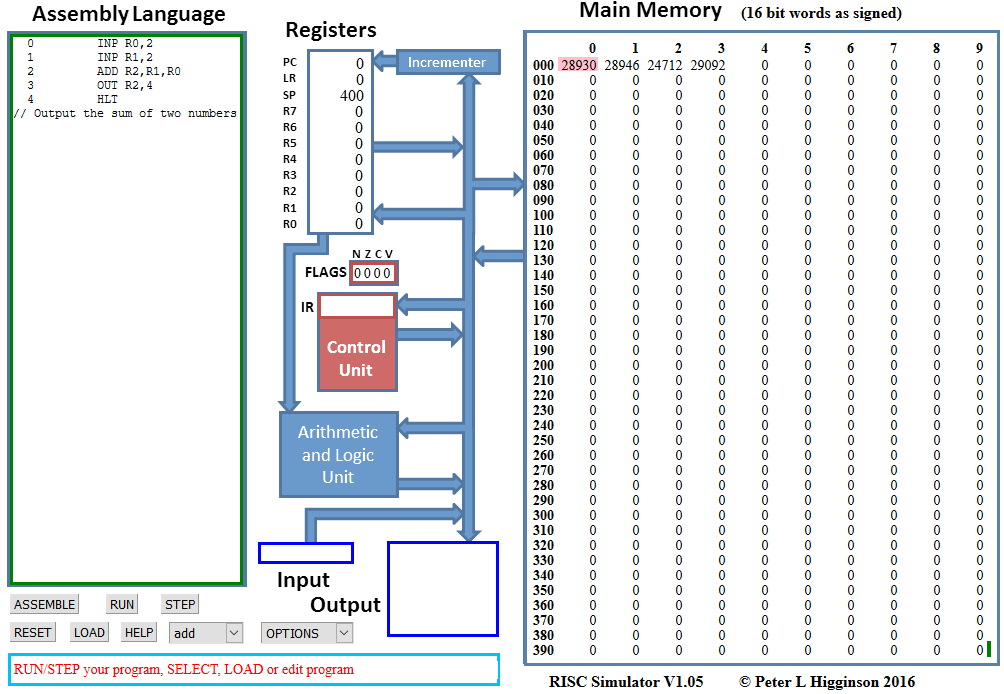
\includegraphics[scale=0.5]{images/RISC.png}
\end{center}

Trois registres ont des fonctions précises.

\begin{itemize}
	\item Le registre PC : Compteur Programme (adresse de la prochaine instruction).
	\item Le registre LR : Adresse de retour (Link Register).
	\item Le registre SP : Pointeur de pile (Stack Pointer).
\end{itemize}

Quatre drapeaux sont représentés (N : Négatif, Z : zéro, C : retenue, V : Dépassement).

\begin{multicols}{3}
\centering

Algorithme

Assembleur

Machine
\end{multicols}

\begin{multicols}{3}
\centering

\begin{algorithm}[H]
$R_1\leftarrow10$\;
\Tq {$R_1\neq0$}
  {   $R_1\leftarrow R_1-1$\;
      Affiche $R_1$\;
  }
\end{algorithm}

\begin{minted}{asm}
        MOV R1,#10
debut:  CMP R1,#0
        BEQ fin
        SUB R1,#1
        OUT R1,4
        BRA debut
fin:    HLT
\end{minted}

\begin{minted}{asm}
0010100100001010
0010000100000000
1000001000000110
0001100100000001
0111000110010100
1000000000000001
0000000000000000
\end{minted}
\end{multicols}

Certaines opérations fondamentales sont disponibles dans la plupart des jeux d'instructions.

\begin{itemize}
	\item Pour le traitement des données. (Calculs arithmétiques, logiques et comparaisons.)
	
	\item Pour le transfert des données (des registres depuis ou vers la mémoire).
	
	\item Pour réaliser des << branchements >>. (Saut non incrémentale d'adresses dans le programme.)
\end{itemize}

Exemples disponibles avec le simulateur : 

(liste complète \href{peterhigginson.co.uk/RISC/instruction_set.pdf}{peterhigginson.co.uk/RISC/instruction\_set.pdf})

\begin{itemize}
	\item Traitement des données.
	
	\asminline{ADD R1,#10} ajoute le nombre 10 au registre R1 ($R_1 \leftarrow R_1+10$),
	
	\asminline{ADD R1,R2,R3} ajoute R3 à R2 et place la somme dans R1 ($R_1 \leftarrow R_1+R_2$),
	
	\asminline{MOV R1, R2} place la valeur de R2 dans R1  ($R_1 \leftarrow R_2$),
	
	\asminline{CMP R1, #27} compare la valeur de R1 avec 27 (Résultats dans les drapeaux).
	
	\item Transfert des données.
   	
	\asminline{STR R1,10} enregistre le contenu du registre R1 en mémoire à l'adresse 10.
   	
	\asminline{LDR R1,10} charge dans le registre R1 le contenu de la mémoire à l'adresse 10.
	
	\item Branchements.
	
	\asminline{BRA 7} saute à l'instruction en mémoire à l'adresse mémoire 7.
	
	\asminline{BRA ici} saute à l'instruction en mémoire à l'adresse du label \asminline{ici:}.
	
	À partir de la valeur des drapeaux, saut d'instruction si
	
	\quad \asminline{BEQ ici} il y a égalité ; \asminline{BNE ici} il n'y a pas égalité
	
	\quad \asminline{BGT ici} la valeur est plus grande ; \asminline{BLT ici} la valeur est plus plus petite.
\end{itemize}


\chapter{Réseau}

\section{Introduction}

\Cours{{\bfseries Réseaux}

Un réseau est un ensemble de \emph{matériels}, connectés de manière à pouvoir \emph{échanger} des données numériques et \emph{partager} des ressources.}


\begin{center}
\begin{tikzpicture}[xscale=1.5]
\coordinate(I)at(0,0);
\coordinate(R0)at($(I)+(1.5cm, 0)$);
\coordinate(C0)at($(R0)+(2cm, -1cm)$);
\coordinate(R)at($(C0)+(-0.75cm, 2cm)$);
\coordinate(C)at($(C0)+(1.5cm, -0.75cm)$);
\coordinate(S0)at($(C0)+(1cm, 1.5cm)$);
\coordinate(S)at($(C0)+(2.5cm, 0.75cm)$);
\coordinate(W)at($(C0)+(-1.5cm, -0.75cm)$);
\coordinate(T)at($(W)+(-1cm, -1.5cm)$);
\coordinate(P)at($(C)+(1.5cm, 0)$);
\coordinate(O1)at($(C)+(-2cm, -1.5cm)$);
\coordinate(O2)at($(C)+(0, -1.5cm)$);
\coordinate(O3)at($(C)+(2cm, -1.5cm)$);
%
\draw(I)--(R0)--(C0)--(S0)(C0)--(S)++(-0.25,1.25)node[right]{\bfseries\large\emph{Réseau local (LAN)}}
     (C0)--(R)--++(-1cm,0)node[left]{liaison étendue WAN}(W)--(C0)--(C)--(P)(C)--(O1)(C)--(O2)(C)--(O3);
\node[cloud, cloud puffs = 15, draw, minimum width = 1.5cm, minimum height = 1.25cm, fill = white]at(I){};
\node[]at(I){\footnotesize Internet};
\node[]at(R0){\routeur};\node[right = 0.5cm]at(R0){routeur};
\node[]at(C0){\switch};\node[right = 0.5cm]at(C0){commutateur};
\node[]at(R){\routeur};\node[right = 0.5cm]at(R){routeur};
\node[]at(C){\switch};\node[left = 0.5cm]at(C){commutateur};
\node[]at(S0){\serveur};\node[right = 0.4cm]at(S0){serveur};
\node[]at(S){\serveur};\node[right = 0.4cm]at(S){serveur};
\node[]at(P){\imprimante};\node[right = 0.4cm, text width=2.5cm]at(P){imprimante\\réseau};
\node[]at(O1){\ordinateur};\node[below = 0.4cm]at(O1){ordinateur};
\node[]at(O2){\ordinateur};\node[below = 0.4cm]at(O2){ordinateur};
\node[]at(O3){\ordinateur};\node[below = 0.4cm]at(O3){ordinateur};
\node[yshift=0.5cm]at(W){\accesWiFi};\node[left = 0.5cm,yshift=0.1cm]at(W){concentrateur WiFi};
\node[]at(T){\telephone};\node[below = 0.4cm]at(T){téléphone};
\draw[](T)++(0.1,0.25)++(20:0.25) arc (20:80:0.25);
\draw[](T)++(0.1,0.25)++(20:0.5) arc (20:80:0.5);
\draw[](T)++(0.1,0.25)++(20:0.75) arc (20:80:0.75);
\end{tikzpicture}
\end{center}

On distingue différents types de réseaux selon leurs tailles (nombre de matériels connectés), leurs structures (façon de les connecter), leurs étendues géographiques (LAN < WAN )...

\noindent\date{1969} Transmission du premier message << login >> sur ARPANET.

(ARPANET - Advanced Research Projects Agency Network - est le premier réseau, développé aux États-Unis, entre des universités.)

\begin{itemize}
	\item en 1981 : 213 machines connectés sur Internet.
	\item en 1989: \np{100000} machines connectés - $1^{\text{er}}$ navigateur web graphique (par le CERN).

(CERN : Conseil européen pour la recherche nucléaire.)
	\item De nos jours, il y en a des dizaines de milliards.
\end{itemize}

\section{Réseaux locaux}

\subsection{Définition}

\Cours{{\bfseries Réseau local (RL) - Local Area Network (LAN)}

C'est un réseau de taille réduite couvrant un domaine privé (entreprises, administrations, universités,...)}

\noindent\date{02/1980} Constitution du comité IEEE  802, pour standardiser les transmissions d'informations.

(IEEE : Institute of Electrical and Electronics Engineers)

En particulier, pour les réseaux locaux :
\begin{multicols}{2}
\begin{itemize}
	\item Ethernet - filaire (IEEE 802.3) ;
	\item 1996 Fast Ethernet (IEEE 802.14) ;
	\item WLAN - réseau sans fil (IEEE 802.11) ;
	\item 2002 Bluetooth (802.15) ; ...
\end{itemize}
\end{multicols}

\subsection{Matériel}

Les réseaux Ethernet sont constitués d'ordinateurs et autres machines possédant une carte réseau, reliés, par des câbles Ethernet, à un ou plusieurs commutateurs (switchs), eux-mêmes reliés entre eux.

\begin{center}\begin{tabular}{ccc}
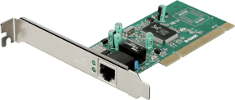
\includegraphics[height=2cm]{images/carteEths.jpg} & 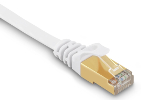
\includegraphics[height=2cm]{images/rj45s.jpg} & 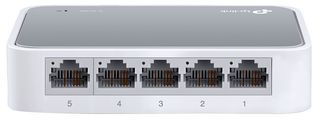
\includegraphics[height=2cm]{images/switch.jpg} \\
carte réseau & câble Ethernet & commutateur (switch) \\
\end{tabular}\end{center}

{\bfseries Pour aller plus loin : } 

Pour relier de tels réseaux entre eux, on utilise des routeurs, possédant, eux, plusieurs cartes réseaux. D'autres supports existent alors, comme la fibre optique.

\begin{center}\begin{tabular}{ccc}
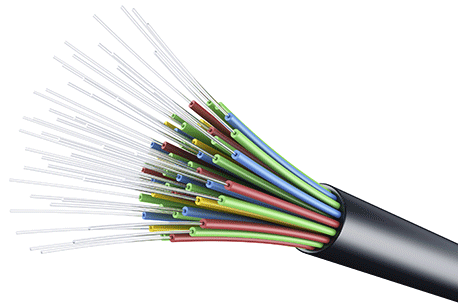
\includegraphics[height=2cm]{images/fibre.png} & 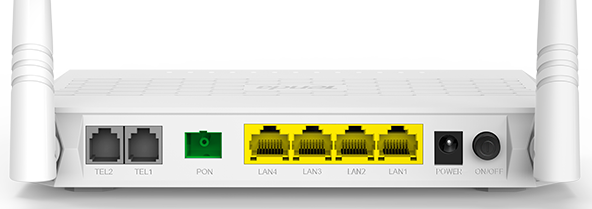
\includegraphics[height=2cm]{images/routeur.png} & 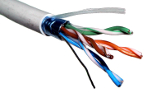
\includegraphics[height=2cm]{images/torsades.jpg}\\
fibre optique & routeur & câble Ethernet \\
\end{tabular}\end{center}

\subsection{Adressage physique (couche Réseau)}

\Cours{{\bfseries Adresse physique (MAC)} (MAC : Media Access Control) 

C'est un identifiant, unique dans le monde, pour chaque carte réseau.}

Elle se présente sous la forme de 6 octets (48 bits), en notation hexadécimale, séparés par un double point ou un tiret. Exemple : \texttt{88-AD-43-F7-26-F8}.

\medskip

Les adresses physiques désignent, dans une \emph{trame}, les protagonistes directs d'un transport de datagramme sur le réseau.

Trame : \fbox{$\cdots$ @MAC-source ; @MAC-destination $\cdots$ \fbox{datagramme} $\cdots$}

C'est chaque bit de cette trame qui est transmis physiquement sur le réseau.

Un \emph{commutateur} (switch) \raisebox{-1ex}{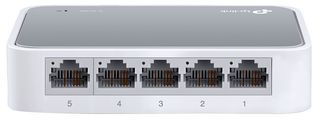
\includegraphics[height=1.5em]{images/switch.jpg}} \raisebox{-1.5ex}{\tikz\node[scale=0.9]{\switch};} est capable de décoder cette trame.
\begin{itemize}
    \item Il met à jour sa liste, appelée \emph{table SAT}, des machines qui lui sont connectées.
    \item Il ne transmet la trame qu'au destinataire.
\end{itemize}


\subsection{Adressage réseaux (couche Internet)}

\Cours{{\bfseries Adresse IP} (IP : Internet Protocol)

 C'est un identifiant (l'adresse), unique dans un réseau (le réseau public : internet, ou un réseau privé), pour chaque carte réseau.}
 
Elle se présente (en version 4) sous la forme de 4 octets (32 bits), en notation décimale, séparés par un  point. Exemple : \texttt{192.168.1.67}

\medskip

On peut demander ses propres identifiants en ligne de commande :

\smallskip

\cmd{ipconfig} (Windows)

\begin{shell}
C:\>ipconfig /all

Carte Ethernet Ethernet:

   Adresse physique . . . . . . . . . . . : 88-AD-43-F7-26-F8
   Adresse IPv4. . . . . . . . . . . . . .: 192.168.1.67
\end{shell}

\smallskip

\cmd{ip} (Unix)

\begin{shell}
moi@ici:~$ ip addr show

2: enp0s3:
    link/ether 88:AD:43:F7:26:F8 brd ff:ff:ff:ff:ff:ff
    inet 192.168.1.67/24 brd 192.168.1.255 scope global dynamic enp0s3
\end{shell}
%$

\medskip

Pour tester si un équipement est joignable sur un réseau IP, on peut utiliser :

\smallskip

\cmd{ping} (Windows / Unix)

\begin{shell}
C:\>ping 192.168.1.1

Envoi d’une requête 'Ping'  192.168.1.1 avec 32 octets de données :
Réponse de 192.168.1.1 : octets=32 temps<1ms TTL=64
...

C:\>ping 192.168.1.7

Envoi d’une requête 'Ping'  192.168.1.7 avec 32 octets de données :
Réponse de 192.168.1.67 : Impossible de joindre l’hôte de destination.
\end{shell}


\medskip

Elle désigne, dans un \emph{datagramme}, les protagonistes initiateur et final et permettent l'acheminement (le routage) de paquets de données. 

Datagramme : \fbox{$\cdots$ @IP-initiale ; @IP-finale $\cdots$ \fbox{paquet}}

C'est l'assemblage de plusieurs paquets qui forme le message envoyé et reçu par les applications.
\subsection{Communication entre applications}


Le but de tout réseau est de pouvoir faire communiquer des logiciels sur des ordinateurs distants. Pour transporter ses données :

\begin{itemize}
	\item l'application fait appel à un protocole de transport : TCP (Transmission Control Protocol) qui va faire des paquets de données (numérotés) à envoyer.
	\item Chaque paquet reçoit l'adresse IP source et l'adresse IP destination,  pour former un datagramme, routable sur internet.
	\item Chaque échange sur les réseaux se fait par trames de données, en identifiant les voisins, de proche en proche, par leur adresse MAC.
\end{itemize}  

\begin{center}\begin{tikzpicture}[align=center, inner sep=1pt]
\node[text width = 3.5cm, inner sep=1ex](T2){{\bfseries Modèle TCP/IP} \\ (Protocole possible)};
\node[text width = 3.5cm, xshift = -5cm](T1){\bfseries Ordinateur A};
\node[text width = 3.5cm, xshift = 5cm](T3){\bfseries Ordinateur B};
%
\node[text width = 5cm, yshift = -1.5cm](A1)at(T1){message \\ \rule{2cm}{0.25cm}};
\node[text width = 4cm, yshift = -1.5cm, draw, inner sep=1ex](A2)at(T2){Application \\ (HTTP)};
\node[text width = 4cm, yshift = -1.5cm](A3)at(T3){Données utilisateur};
%
\node[text width = 5cm, yshift = -1.5cm](P1)at(A1){paquets \\ \fbox{1\rule{0.35cm}{0.25cm}} \fbox{2\rule{0.35cm}{0.25cm}} \fbox{3\rule{0.35cm}{0.25cm}}};
\node[text width = 4cm, yshift = -1.5cm, draw, inner sep=1ex](P2)at(A2){Transport \\ (TCP)};
\node[text width = 4cm, yshift = -1.5cm](P3)at(A3){Gestion des flux};
%
\node[text width = 5cm, yshift = -1.5cm](I1)at(P1){datagrammes \\ \fbox{@ipA. @ipB. \fbox{2\rule{0.35cm}{0.25cm}}}};
\node[text width = 4cm, yshift = -1.5cm, draw, inner sep=1ex](I2)at(P2){Internet \\ (IP)};
\node[text width = 4cm, yshift = -1.5cm](I3)at(P3){Adressage origine/but};
%
\node[text width = 6cm, yshift = -1.5cm](R1)at(I1){trames \\ \fbox{@MAC \fbox{2a} -} \fbox{@MAC \fbox{2b} -}};
\node[text width = 6cm, yshift = -2.5cm](B)at(I2){$100101101010010010111010101$};
\node[text width = 4cm, yshift = -1.5cm, draw, fill = white, inner sep=1ex](R2)at(I2){Accès Réseau \\ (Ethernet)};
\node[text width = 4cm, yshift = -1.5cm](R3)at(I3){Envoi et reception des données};
%
\draw[latex-latex] (A1.south) -- (P1);
\draw[latex-latex] (A1.south) -- (P1.45);
\draw[latex-latex] (A1.south) -- (P1.135);
\draw[latex-latex] (P1) -- (I1);
\draw[latex-latex] (I1.south) -- (R1.45); 
\draw[latex-latex] (I1.south) -- (R1.135); 
\draw[latex-latex] (R1) to[out=-45,in=180] (B); 
\draw[latex-latex] (A3) -- (P3);
\draw[latex-latex] (P3) -- (I3);
\draw[latex-latex] (I3) -- (R3); 
\draw[latex-latex] (R3) to[out=-90,in=0] (B); 
\end{tikzpicture}\end{center}

{\bfseries Pour aller plus loin : } 

\Cours{{\bfseries Numéro de port} 

 C'est l'identifiant d'une application. Associé à l'adresse IP de l'ordinateur, ils définissent un \emph{socket} qui permet une connexion TCP (Transmission Control Protocol).}
 
 Exemples de ports pré-définis :
 
 \begin{itemize}
 	\item 25 : SMTP (Simple Mail Transfert Protocol)
 	\item 80 : HTTP (HyperText Transfer Protocol)
 	\item 110 : POP3 (Post Office Protocol, version 3) 
 \end{itemize}
 
\subsection{Masque de réseau}

Une adresse IP contient toujours au moins deux informations distinctes : 
\begin{itemize}
	\item l'identifiant du réseau sur lequel est la machine,
	\item et l'identifiant de la machine elle-même sur ce réseau.
\end{itemize}
 
\begin{center}\begin{tikzpicture}
\node[inner sep = 0](IP){\Large\texttt{192.168.1.67}};
\draw[decorate,decoration={brace,raise=0.1cm}](IP.north west) 
     -- ($0.25*(IP.north west)+0.75*(IP.north east)$) node[above=0.2cm,pos=0.2] {Réseau \texttt{192.168.1.0}};
\draw[decorate,decoration={brace,raise=0.1cm}]($0.2*(IP.north west)+0.8*(IP.north east)$)
    node[above right,yshift=0.2cm] {machine  \texttt{67}} -- (IP.north east)  ;
\end{tikzpicture}\end{center}

Plus précisément :

\begin{center}\begin{tikzpicture}
\node[inner sep = 0](IP){\Large\texttt{1100 0000 . 1010 1000 . 0000 0001 . 0100 0011}};
\draw[decorate,decoration={brace,raise=0.1cm}](IP.north west) 
     -- ($0.26*(IP.north west)+0.74*(IP.north east)$) node[above=0.2cm,pos=0.5] {Réseau \texttt{192.168.1.0}};
\draw[decorate,decoration={brace,raise=0.1cm}]($0.205*(IP.north west)+0.795*(IP.north east)$)
     -- (IP.north east)node[above=0.2cm,pos=0.5] {machine  \texttt{67}}  ;
\end{tikzpicture}\end{center}

Mais le nombre de bits attribués au réseau peut être différent, par exemple :

\begin{center}\begin{tikzpicture}
\node[inner sep = 0](IP){\Large\texttt{1100 0000 . 1010 1000 . 0000 0001 . 0100 0011}};
\draw[decorate,decoration={brace,raise=0.1cm}](IP.north west) 
     -- ($0.105*(IP.north west)+0.895*(IP.north east)$) node[above=0.2cm,pos=0.5] {Réseau \texttt{192.168.1.64}};
\draw[decorate,decoration={brace,raise=0.1cm}]($0.095*(IP.north west)+0.905*(IP.north east)$)
     -- (IP.north east)node[above=0.2cm,pos=0.5] {machine  \texttt{3}}  ;
\end{tikzpicture}\end{center}

\Cours{{\bfseries Masque de réseau} 

Le masque d'un réseau se présente sous la forme d'une adresse IP pour laquelle tous les bits composant le réseau sont égaux à 1 et tous les autres égaux à 0.

Elle permet, avec l'opération binaire \pythoninline{&} de déterminer le réseau correspondant à l'adresse IP d'une machine.}

\begin{center}\begin{tikzpicture}
\node[inner sep = 0](IP){\large\texttt{1100 0000 . 1010 1000 . 0000 0001 . 0100 0011}};
\node[inner sep = 0,below=1ex](M)at(IP.south){\large\texttt{1111 1111 . 1111 1111 . 1111 1111 . 1111 0000}};
\node[left=1em]at(M.west){\large\texttt{\&}};
\node[inner sep = 0,below=2ex](R)at(M.south){\large\texttt{1100 0000 . 1010 1000 . 0000 0001 . 0100 0000}};
\draw($(M.south west)+(-2em,-1ex)$)--($(M.south east)+(1em,-1ex)$);
\end{tikzpicture}\end{center}

Sur l'exemple ci-dessus, le masque est \texttt{255.255.255.240}.

Pour simplifier, on peut juste donner le nombre de bits à 1 pour le masque. Par rapport à l'exemple précédent, on peut distinguer \texttt{192.168.1.67/24} et \texttt{192.168.1.67/28} qui ne sont pas sur le même réseau.

Cette distinction est importante car seules les machines partageant le même réseau peuvent communiquer directement ou à travers un commutateur.

\section{Contrôle de flux}

Les messages qui transitent sur les réseaux sont découpés en morceaux (dès la prise en charge par le protocole TCP, qui en fait des paquets). Il peut donc s'avérer important que la source s'assure de la bonne réception de chaque morceau dans le bon ordre pour valider l'envoi (et sinon renvoyer l'information).

On représente la situation par deux axes verticaux représentant l'écoulement du temps au niveau de la source et du destinataire des messages, séparé par un espace représentant le réseau de communication. On symbolise le routage des données par des flèches allant d'une verticale à l'autre. Idéalement :

\begin{center}\begin{tikzpicture}\small
\fill[black!5](-1.5cm,-4cm)rectangle(1.5cm,0);
\node{Réseau};
\draw[line width = 2pt](-1.5cm,-4cm)--(-1.5cm,0)node[above]{Source};
\draw[line width = 2pt](1.5cm,0)node[above]{Destinataire}--(1.5cm,-4cm);
\draw[-latex](-1.5cm,-0.5cm)node{$\bullet$}node[left]{Émet morceau 1}--(1.5cm,-1cm)node[right]{Reçoit morceau 1};
\draw[-latex](-1.5cm,-1.5cm)node{$\bullet$}node[left]{Émet morceau 2}--(1.5cm,-2cm)node[right]{Reçoit morceau 2};
\draw[-latex](-1.5cm,-2.5cm)node{$\bullet$}node[left]{Émet morceau 3}--(1.5cm,-3cm)node[right]{Reçoit morceau 3};
\draw[-latex](-5,0)--(-5,-4)node[midway,above,sloped]{écoulement du temps};
\node[]at(0,-3.75){\checkmark};
\end{tikzpicture}\end{center}

On souhaite éviter la perte d'un morceau ou l'arrivée des morceaux dans le désordre :

\begin{center}\begin{tikzpicture}\small
\fill[black!5](-1.5cm,-4cm)rectangle(1.5cm,0);
\draw[line width = 2pt](-1.5cm,-4cm)--(-1.5cm,0)node[above]{Source};
\draw[line width = 2pt](1.5cm,0)node[above]{Destinataire}--(1.5cm,-4cm);
\draw[-latex](-1.5cm,-0.5cm)node{$\bullet$}node[left]{1}--(1.5cm,-1cm)node[right]{1};
\draw[-](-1.5cm,-1.5cm)node{$\bullet$}node[left]{2}--(0cm,-1.75cm)node{\textsf{X}};
\draw[-latex](-1.5cm,-2.5cm)node{$\bullet$}node[left]{3}--(1.5cm,-3cm)node[right]{3};
\node[]at(0,-3.75){\textsf{X}};
\end{tikzpicture} \qquad \begin{tikzpicture}\small
\fill[black!5](-1.5cm,-4cm)rectangle(1.5cm,0);
\draw[line width = 2pt](-1.5cm,-4cm)--(-1.5cm,0)node[above]{Source};
\draw[line width = 2pt](1.5cm,0)node[above]{Destinataire}--(1.5cm,-4cm);
\draw[-latex](-1.5cm,-0.5cm)node{$\bullet$}node[left]{1}--(1.5cm,-2.5cm)node[right]{1};
\draw[-latex](-1.5cm,-1.5cm)node{$\bullet$}node[left]{2}--(1.5cm,-2cm)node[right]{2};
\draw[-latex](-1.5cm,-2.5cm)node{$\bullet$}node[left]{3}--(1.5cm,-3cm)node[right]{3};
\node[]at(0,-3.75){\textsf{X}};
\end{tikzpicture}\end{center}

\subsection{Envoyer et attendre (Send and Wait)}

Le principe est le suivant.

\begin{itemize}
	\item La source n'envoie qu'un morceau à la fois et attend un \emph{aquittement} (ACK) du destinataire.
	\item Le destinataire n'envoie un ACK que s'il reçoit un morceau en bon état.
	\item Après un délai pré-établi (timeout) sans ACK, la source renvoie le même morceau.
	\item Après réception d'un ACK, la source envoie le morceau suivant.
\end{itemize}
\begin{center}\begin{tikzpicture}\small
\fill[black!5](-1.5cm,-4cm)rectangle(1.5cm,0);
\draw[line width = 2pt](-1.5cm,-4cm)--(-1.5cm,0)node[above]{Source};
\draw[line width = 2pt](1.5cm,0)node[above]{Destinataire}--(1.5cm,-4cm);
\draw[-latex](-1.5cm,-0.5cm)node{$\bullet$}node[left]{1}--(1.5cm,-0.7cm)node[right]{1};
\draw[-latex](1.5cm,-0.75cm)--(-1.5cm,-0.95cm)node[midway,sloped,inner sep=1pt,fill=black!5,draw]{\footnotesize ACK};
\draw[-](-1.5cm,-1cm)node{$\bullet$}node[left]{2}--(0cm,-1.2cm)node{\textsf{X}};
\draw[-latex](-2,-1)--(-2,-2)node[left]{timeout}--(-1.8,-2);
\draw[-latex](-1.5cm,-2cm)node{$\bullet$}node[left]{2}--(1.5cm,-2.2cm)node[right]{2};
\draw[-latex](1.5cm,-2.25cm)--(-1.5cm,-2.45cm)node[midway,sloped,inner sep=1pt,fill=black!5,draw]{\footnotesize ACK};
\draw[-latex](-1.5cm,-2.5cm)node{$\bullet$}node[left]{3}--(1.5cm,-2.7cm)node[right]{3};
\node[]at(0,-3.75){\checkmark};
\end{tikzpicture} \qquad \begin{tikzpicture}\small
\fill[black!5](-1.5cm,-4cm)rectangle(1.5cm,0);
\draw[line width = 2pt](-1.5cm,-4cm)--(-1.5cm,0)node[above]{Source};
\draw[line width = 2pt](1.5cm,0)node[above]{Destinataire}--(1.5cm,-4cm);
\draw[-latex](-1.5cm,-0.5cm)node{$\bullet$}node[left]{1}--(1.5cm,-2cm)node[right]{1};
\draw[-latex](-2,-0.5)--(-2,-1.5)node[left]{timeout}--(-1.8,-1.5);
\draw[-latex](-1.5cm,-1.5cm)node{$\bullet$}node[left]{1}--(1.5cm,-1.7cm)node[right]{1};
\draw[-latex](1.5cm,-1.75cm)--(-1.5cm,-2.2cm)node[midway,sloped,inner sep=1pt,fill=black!5,draw]{\footnotesize ACK};
\draw[-latex](-1.5cm,-2.25cm)node{$\bullet$}node[left]{2}--(1.5cm,-2.45cm)node[right]{2};
\draw[-latex](1.5cm,-2cm)--(-1.5cm,-2.65cm)node[midway,sloped,inner sep=1pt,fill=black!5,draw]{\footnotesize ACK};
\node[]at(0,-3.75){\textsf{X}};
\end{tikzpicture}\end{center}

Ça ne solutionne qu'une partie du problème.

\subsection{Le bit alterné}

Pour mettre de l'ordre dans les morceaux reçus, on ne peut pas vraiment se passer de les numéroter. L'idée du bit alterné, est de ne les numéroter que sur un bit (par économie) que l'on fait alterner entre 0 et 1, en envoi et dans les acquittements.

Notons \texttt{T0} (ou \texttt{T1}) une trame envoyée avec le bit à 0 (ou 1).

L'acquittement demandera la trame suivante en renvoyant le bit opposé: \texttt{A1} (ou \texttt{A0}) l'acquittement correspondant : 

\begin{multicols}{2}
\begin{center}
On résout le problème précédent :

\begin{tikzpicture}\small
% Mise en place
\fill[black!5](-1.5cm,-4cm)rectangle(1.5cm,0);
\draw[line width = 2pt](-1.5cm,-4cm)--(-1.5cm,0)node[above]{Source};
\draw[line width = 2pt](1.5cm,0)node[above]{Destinataire}--(1.5cm,-4cm);
% Première trame
\draw[-latex](-1.5cm,-0.5cm)node{$\bullet$}node[left]{1}--(1.5cm,-2cm)node[pos=0.33,sloped,inner sep=1pt,fill=white,draw]{\footnotesize T0}node[right]{\textsf{X}};
\draw[-latex](-2,-0.5)--(-2,-1.5)node[left]{timeout}--(-1.8,-1.5);
% Première trame bis
\draw[-latex](-1.5cm,-1.5cm)node{$\bullet$}node[left]{1}--(1.5cm,-1.7cm)node[pos=0.33,sloped,inner sep=1pt,fill=white,draw]{\footnotesize T0}node[right]{1};
\draw[-latex](1.5cm,-1.75cm)--(-1.5cm,-2.2cm)node[pos=0.33,sloped,inner sep=1pt,fill=white,draw]{\footnotesize A1};
\draw[-latex](1.5cm,-2.05cm)--(-1.5cm,-2.6cm)node[pos=0.33,sloped,inner sep=1pt,fill=white,draw]{\footnotesize A1};
% Seconde trame
\draw[-latex](-1.5cm,-2.25cm)node{$\bullet$}node[left]{2}--(1.5cm,-2.6cm)node[pos=0.25,sloped,inner sep=1pt,fill=white,draw]{\footnotesize T1}node[right]{2};
\draw[-latex](1.5cm,-2.65cm)--(-1.5cm,-3cm)node[pos=0.33,sloped,inner sep=1pt,fill=white,draw]{\footnotesize A0};
\node[]at(0,-3.75){\checkmark};
\end{tikzpicture}


Mais pas tous les problèmes :

\begin{tikzpicture}\small
% Mise en place
\fill[black!5](-1.5cm,-4cm)rectangle(1.5cm,0);
\draw[line width = 2pt](-1.5cm,-4cm)--(-1.5cm,0)node[above]{Source};
\draw[line width = 2pt](1.5cm,0)node[above]{Destinataire}--(1.5cm,-4cm);
% Première trame
\draw[-latex](-1.5cm,-0.5cm)node{$\bullet$}node[left]{1}--(1.5cm,-2cm)node[pos=0.33,sloped,inner sep=1pt,fill=white,draw]{\footnotesize T0}node[right]{\textsf{X}};
\draw[-latex](-2,-0.5)--(-2,-1.5)node[left]{timeout}--(-1.8,-1.5);
% Première trame bis
\draw[-latex](-1.5cm,-1.5cm)node{$\bullet$}node[left]{1}--(1.5cm,-1.7cm)node[pos=0.33,sloped,inner sep=1pt,fill=white,draw]{\footnotesize T0}node[right]{1};
\draw[-latex](1.5cm,-1.75cm)--(-1.5cm,-2.2cm)node[pos=0.33,sloped,inner sep=1pt,fill=white,draw]{\footnotesize A1};
\draw[-latex](1.5cm,-2.05cm)--(-1.5cm,-2.6cm)node[pos=0.33,sloped,inner sep=1pt,fill=white,draw]{\footnotesize A1};
% Seconde trame
\draw[-latex](-1.5cm,-2.25cm)node{$\bullet$}node[left]{2}--(1.5cm,-2.6cm)node[pos=0.25,sloped,inner sep=1pt,fill=white,draw]{\footnotesize T1}node[right]{2};
\draw[-latex](1.5cm,-2.65cm)--(-1.5cm,-3cm)node[pos=0.33,sloped,inner sep=1pt,fill=white,draw]{\footnotesize A0};
% Seconde trame bis
\draw[-latex](-1.5cm,-2.65cm)node{$\bullet$}node[left]{2}--(1.5cm,-3.5cm)node[pos=0.15,sloped,inner sep=1pt,fill=white,draw]{\footnotesize T1}node[right]{2};
% Troisième trame
\draw[-latex](-1.5cm,-3.05cm)node{$\bullet$}node[left]{3}--(1.5cm,-3.25cm)node[pos=0.33,sloped,inner sep=1pt,fill=white,draw]{\footnotesize T0}node[right]{3};
\node[]at(0,-3.75){\textsf{X}};
\end{tikzpicture}
\end{center}
\end{multicols}

{\bfseries Pour aller plus loin : } Au niveau du protocole TCP, chaque segment porte un numéro de séquence et un numéro d'acquittement, chacun sur 32 bit pour assurer la bonne réception de l'ensemble dans le bon ordre. 

Par comparaison, le protocole UDP (sans connexion) n'en utilise aucun, pour gagner en rapidité. (Dans un flux vidéo par exemple perdre une partie d'une image est moins grave que de faire une pause pour l'attendre.)

\chapter{Système d'exploitation}

\section{Fonctions d'un système d'exploitation}

\begin{multicols}{2}\Cours{{\bfseries Système d'exploitation}


Un système d'exploitation est l'interface logicielle entre les applications et le matériel informatique. }

(Les utilisateurs utilisent les applications, qui demandent des ressources au système d'exploitation, qui pilote le matériel informatique, le partageant entre différentes applications et différents utilisateurs.)



\begin{tikzpicture}\node[scale=0.49]{\begin{tikzpicture}
\draw[fill=black!5, rounded corners = 5pt](-3,-2.25)rectangle(11,1.25);
\node[text width = 3cm, draw, align=center](A){\raisebox{-1ex}{\rule{0pt}{4ex}}Processeur};
\node[text width = 3cm, draw, align=center, xshift=2.5cm](B)at(A.east){\raisebox{-1ex}{\rule{0pt}{4ex}}Mémoire};
\node[text width = 3cm, draw, align=center, xshift=2.5cm](C)at(B.east){\raisebox{-1ex}{\rule{0pt}{4ex}}Entrées/Sorties};
\node[text width = 12cm, draw, align=center, yshift=-1cm, double arrow](D)at(B.south){Bus de communication};
\draw(A.south)--++($(D.north)-(B.south)$);
\draw(B.south)--++($(D.north)-(B.south)$);
\draw(C.south)--++($(D.north)-(B.south)$);
\node[above=0,inner sep = 0]at(B.north){\huge \bfseries Matériel informatique};
\draw[fill=black!5, rounded corners = 5pt](-3,1.75)rectangle(11,3.25);
\draw[fill=white, rounded corners = 5pt](-2.9,1.85)rectangle(10.9,3.15)node[midway]{\huge \bfseries Système d'exploitation};
\draw[fill=black!5, rounded corners = 5pt](-3,3.75)rectangle(11,5.25)node[midway]{{\huge \bfseries Applications} (processus)};
\draw[fill=black!5, rounded corners = 5pt](-3,5.75)rectangle(11,7.25)node[midway]{{\huge \bfseries Utilisateurs}};
\foreach \x in {0,0.5,...,5} \draw[-latex]({-2.25+\x},1.75)--({-2.25+\x},1.25);
\foreach \x in {0,0.5,...,5} \draw[-latex]({5.25+\x},1.25)--({5.25+\x},1.75);
\foreach \x in {0,0.5,...,5} \draw[-latex]({-2.25+\x},3.75)--({-2.25+\x},3.25);
\foreach \x in {0,0.5,...,5} \draw[-latex]({5.25+\x},3.25)--({5.25+\x},3.75);
\foreach \x in {0,0.5,...,5} \draw[-latex]({-2.25+\x},5.75)--({-2.25+\x},5.25);
\foreach \x in {0,0.5,...,5} \draw[-latex]({5.25+\x},5.25)--({5.25+\x},5.75);
\end{tikzpicture}};
\end{tikzpicture}\end{multicols}

Il existe différentes familles de systèmes d'exploitations.

\noindent\date{1970} Naissance d'UNIX, père des systèmes d'exploitation modernes (macOS, iOS
, Android, Linux sont de la famille UNIX). UNIX étant un système propriétaire (les sources appartiennent à une entreprise et ne sont pas publiques), c'est en clonant ce système (sans utiliser ses sources) que Linux a été écrit (1991).

\noindent\date{1985} Naissance de Windows (sur MS-DOS). Mais il en existe bien d'autres...

\medskip

On peut distinguer quatre grands types de fonctions (trois directement liées au matériel).

\begin{itemize}
	\item La gestion des processus.
	\item La gestion de la mémoire.
	\item La gestion des périphériques d'entrée/sortie.
	\item La gestion du système de fichiers.
\end{itemize}

\section{IHM et Ligne de commande}

\Cours{{\bfseries Interface Homme-Machine}

Une Interface Homme-Machine - IHM est un ensemble de mécanismes, à la fois matériels et logiciels, mis à la disposition des utilisateurs pour leur permettre d'interagir avec un système interactif.}

Cette interface est mise en œuvre sur un \emph{terminal}, ensemble de périphériques d'entrée / sortie, à l'extrémité d'un ordinateur ou d'un réseau. Souvent intégré (clavier, écran tactile, \ldots) mais pas toujours (Terminal bancaire), il peut aussi être virtuel (console  d'un système d'exploitation).

\begin{center}

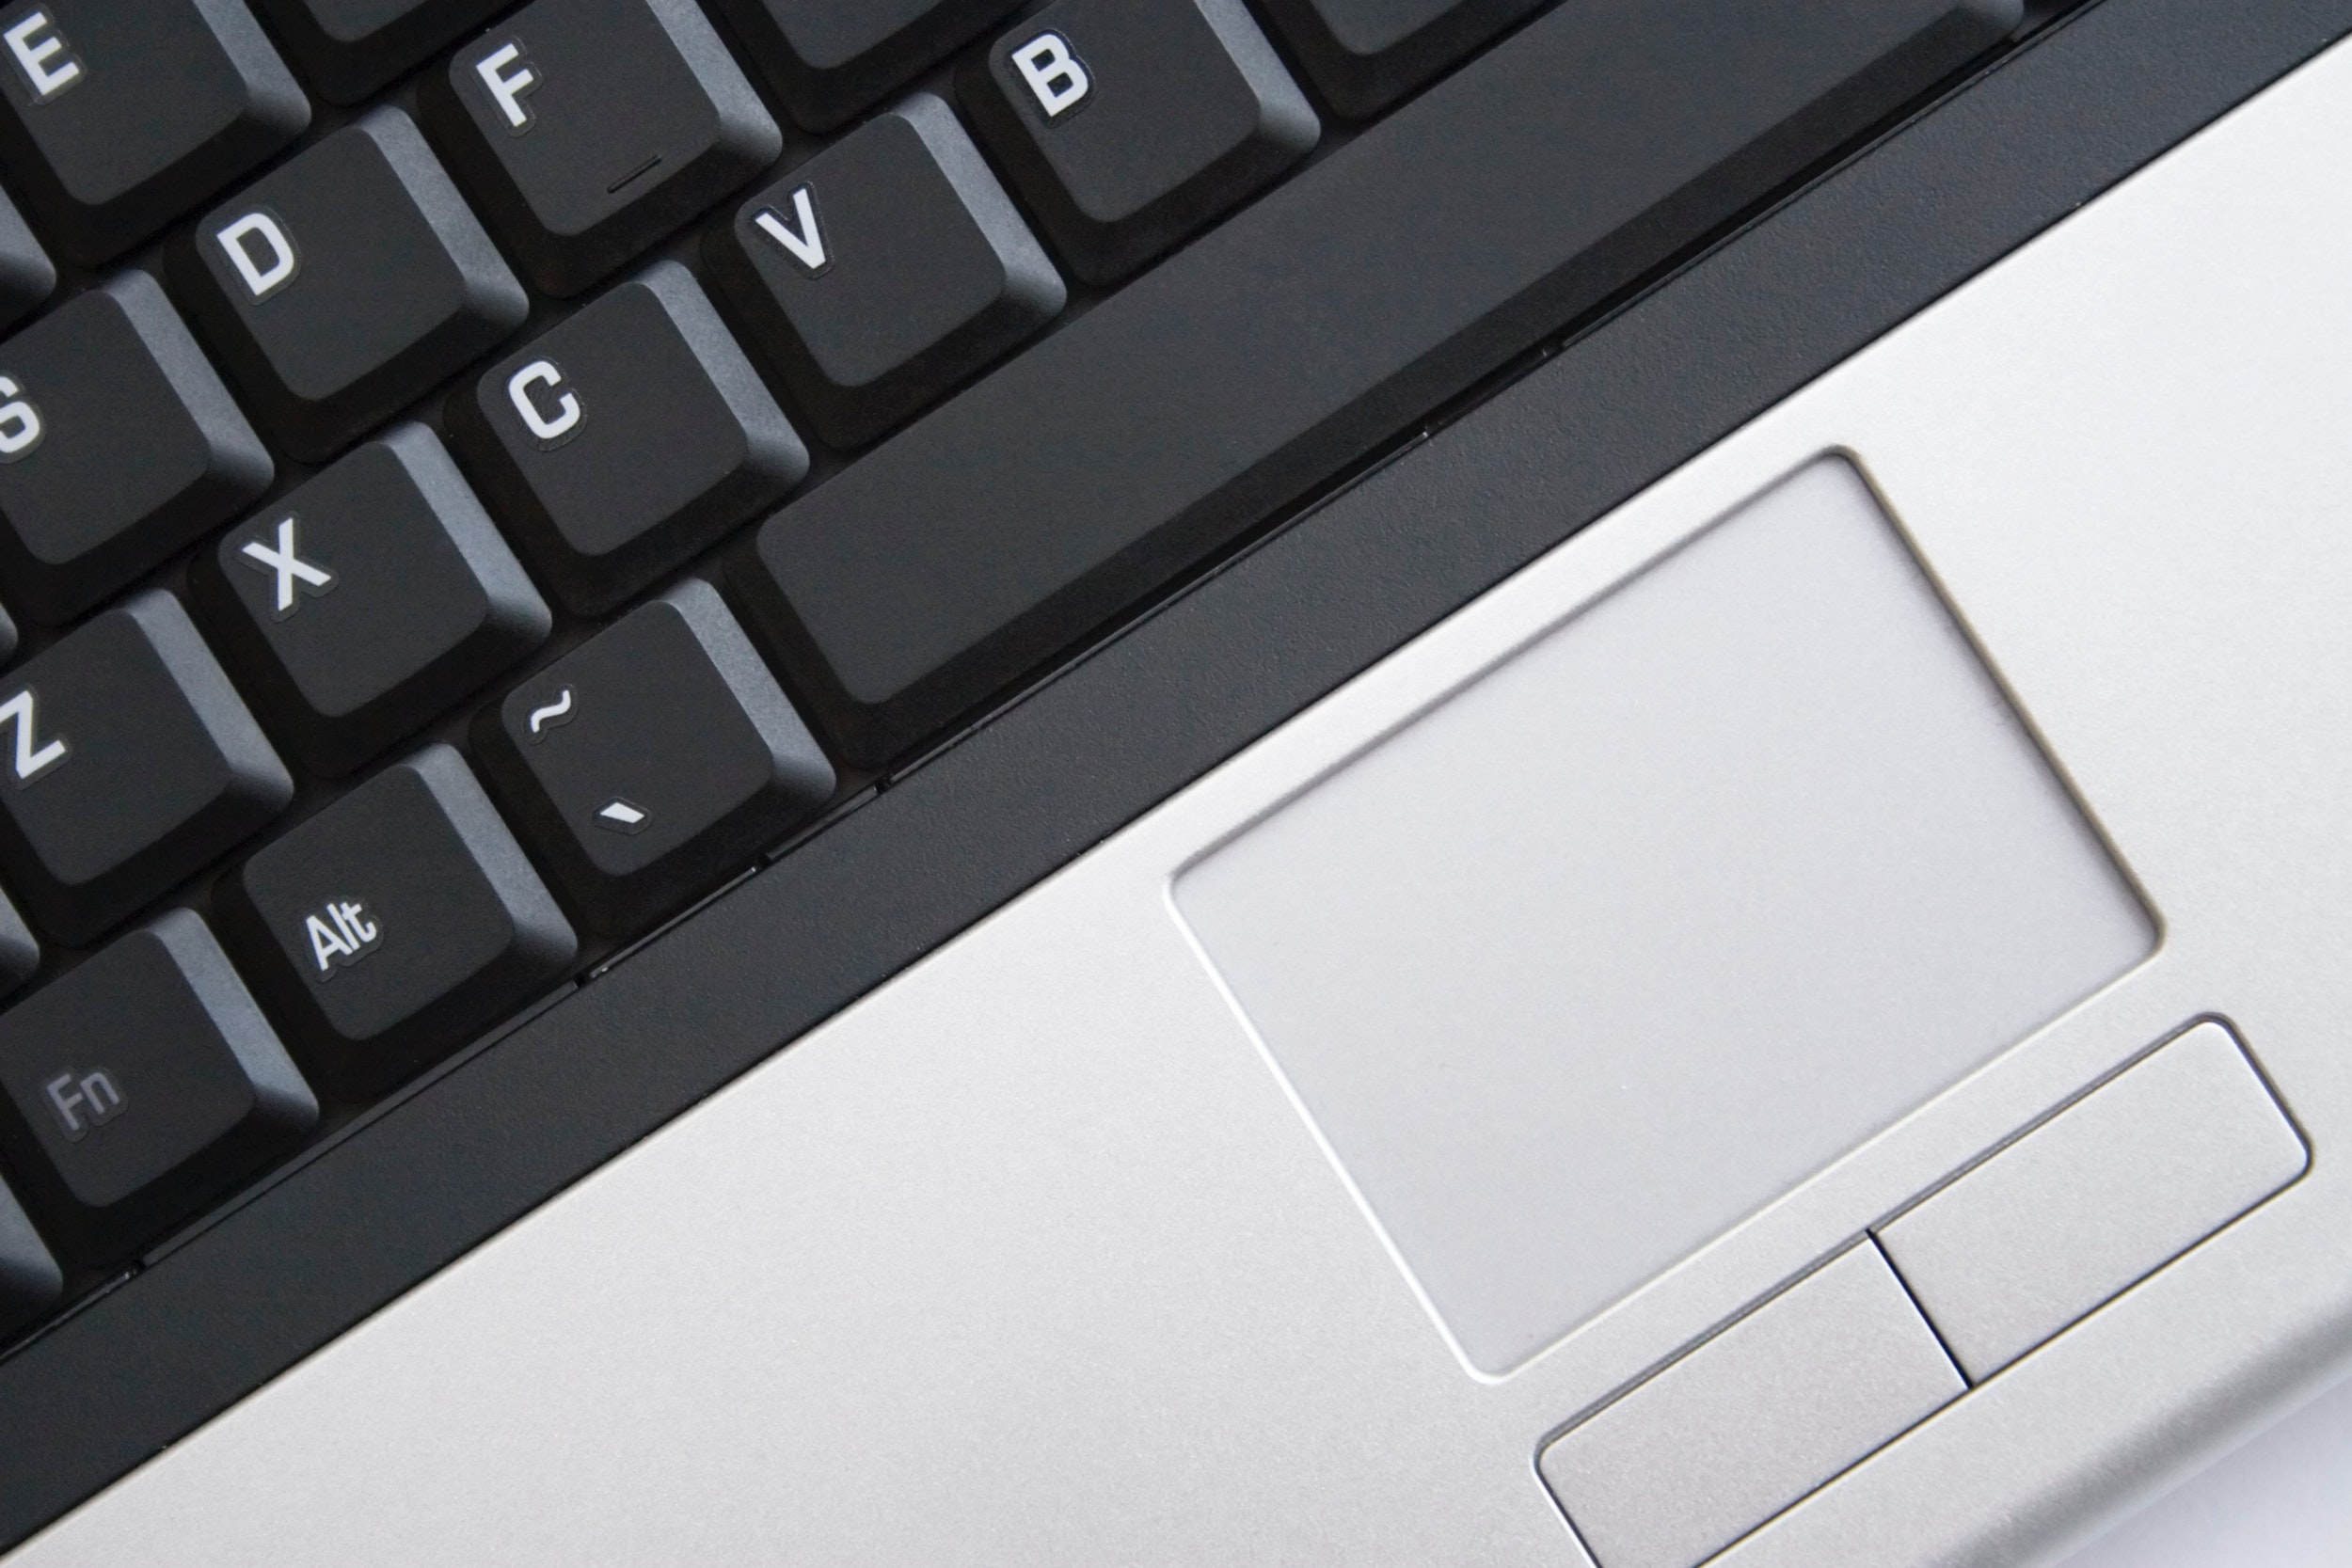
\includegraphics[height=2cm]{images/clavier-cles-ordinateur-portable-93422.jpg}\quad
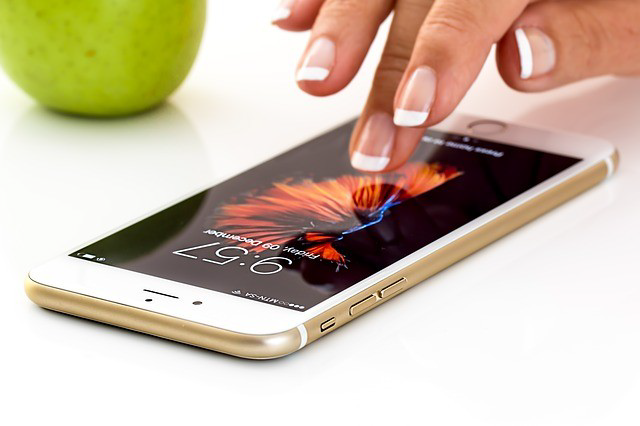
\includegraphics[height=2cm]{images/ecrant.png}\quad
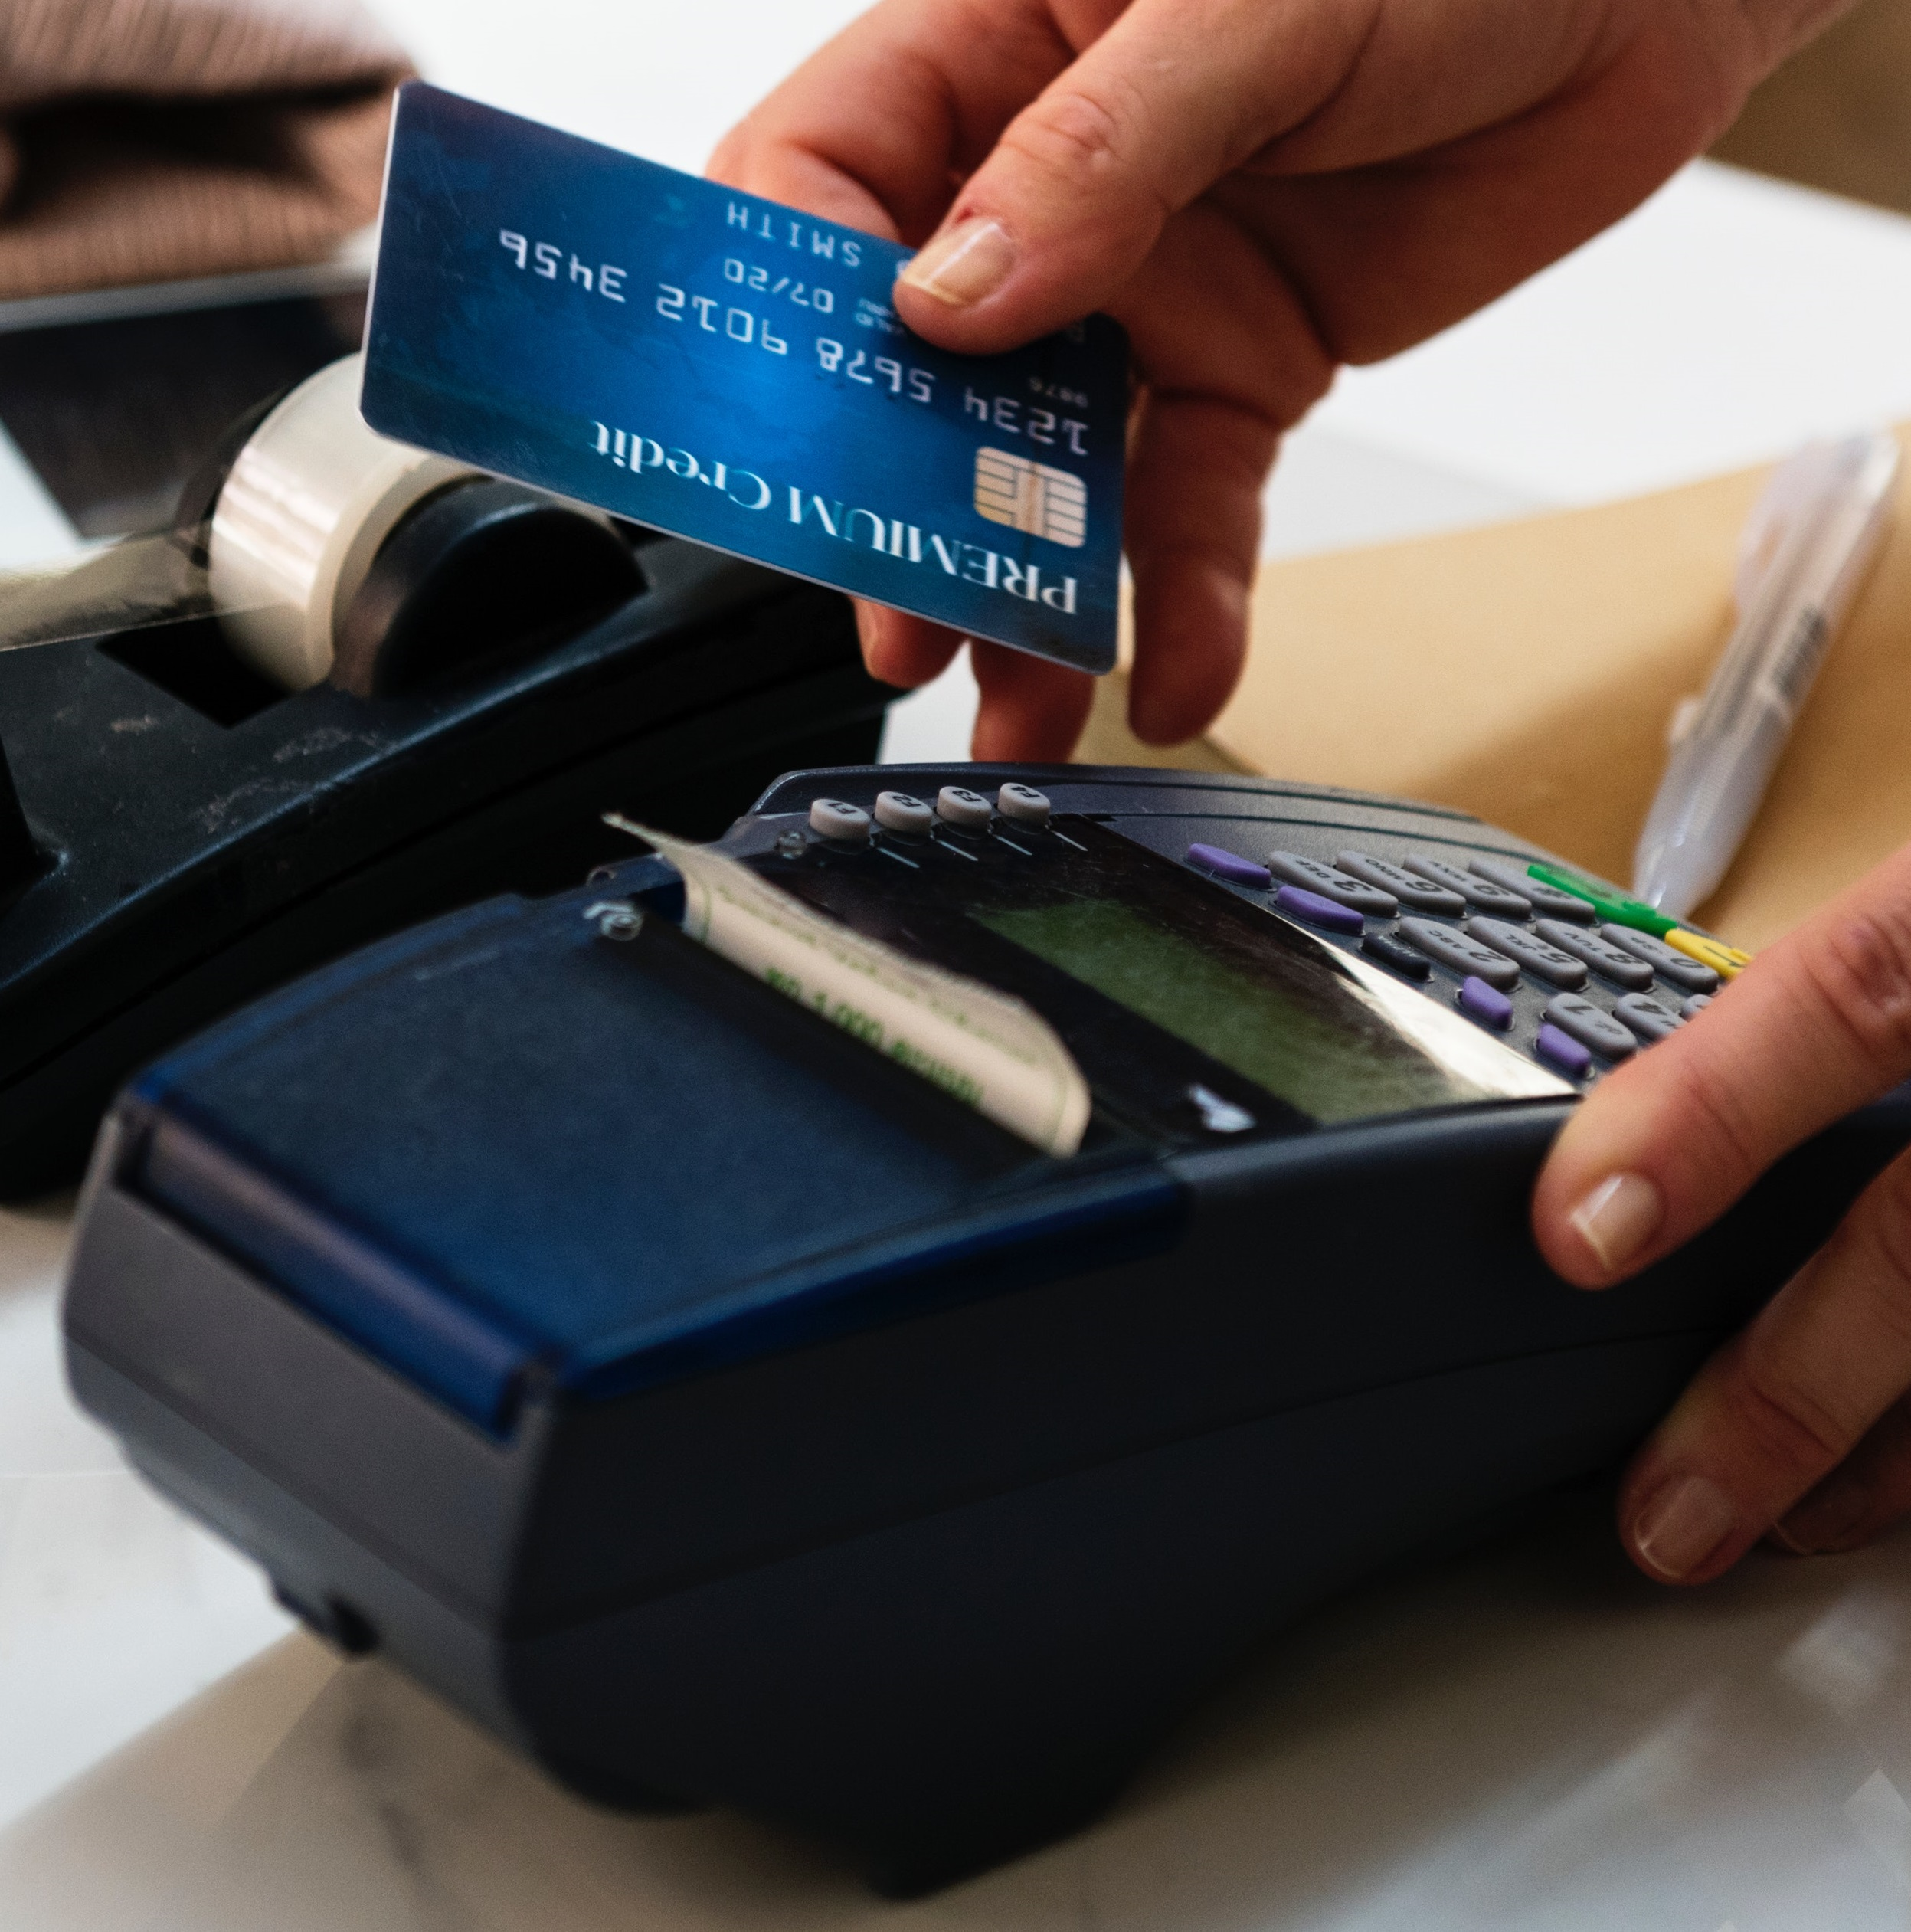
\includegraphics[height=2cm]{images/access-card-cellphone.jpg}\quad
%https://commons.wikimedia.org/wiki/File:Credit_card_terminal_in_Laos.jpg

\includegraphics[height=2cm]{images/bash-148836_960_720}
	
\end{center} 

Sous Ubuntu, c'est l'application  \mintinline{text}{Terminal} ; sous Windows, \mintinline{text}{cmd}.

\begin{multicols}{2}
\noindent\begin{shell}
moi@mongroupe:~$
\end{shell}
%$

L'invite de commande Ubuntu se compose du nom d'utilisateur, de \mintinline{text}{@} et de son groupe, suivi de \mintinline{text}{:} ,
 du répertoire courant (\mintinline{text}{~} pour le répertoire utilisateur) et termine par \mintinline{text}{$}.%$
\columnbreak

\noindent\begin{shell}
C:\Users\moi>
\end{shell}

L'invite de commande << MS-DOS >> de Windows se compose du nom du lecteur, suivi de \mintinline{text}{:}, du répertoire courant et termine par \mintinline{text}{>}.%$
\end{multicols}
%(Exemple motivant : (Win) \texttt{> ren IMG*.jpg ete2019*.jpg})

Une commande est alors composée d'un nom suivi ou non d'options. Les commandes spécifiques au système (que ce soit Ubuntu ou Windows) sont listées par la commande \cmd{help}

Pour effacer la console par exemple : \cmd{clear} (UNIX) ou \cmd{cls} (Windows).

\subsection{Navigation dans l'arborescence des fichiers}

Les données en mémoire sont répertoriées par des fichiers, caractérisés par leur nom, taille, droit d'accès, propriétaire, date de création, de modification, \ldots Ces fichiers sont eux-mêmes répertoriés dans une structure arborescente dont chaque nœud est un dossier. Dans un système UNIX, tout part d'une même racine (root) : \mintinline{text}{/}. Dans un système Windows, il y a une arborescence par disque logique, identifiée par une lettre.

\begin{multicols}{2}
\begin{center}
UNIX

\begin{tikzpicture}
\node(racine)at(0,0){\mintinline{text}{/}};
\node[below left = 1cm, xshift=-0.5cm](bin)at(racine){\mintinline{text}{bin}};
\node[below right = 1cm, xshift=0.5cm](media)at(racine){\mintinline{text}{media}};
\node(home)at($0.5*(bin)+0.5*(media)$){\mintinline{text}{home}};
\node[]at($0.5*(bin)+0.5*(home)$){\ldots};
\node[]at($0.5*(home)+0.5*(media)$){\ldots};
\draw(racine)--(bin);
\draw(racine)--(home);
\draw(racine)--(media);
\draw(bin)++(-0.2cm,-0.75cm)--++(-0.5cm,-0.5cm);
\draw(bin)++(0,-0.75cm)--++(0cm,-0.5cm);
\draw(bin)++(0.2cm,-0.75cm)--++(0.5cm,-0.5cm);
\draw(home)++(-0.2cm,-0.5cm)--++(-0.5cm,-0.75cm);
\draw(home)++(0,-0.5cm)--++(0cm,-0.75cm);
\draw(home)++(0.2cm,-0.5cm)--++(0.5cm,-0.75cm);
\draw(media)++(-0.2cm,-0.75cm)--++(-0.5cm,-0.5cm);
\draw(media)++(0,-0.75cm)--++(0cm,-0.5cm);
\draw(media)++(0.2cm,-0.75cm)--++(0.5cm,-0.5cm);
\node[below=3pt](bin1)at(bin){\scriptsize commandes};\node[below]at(bin1){\scriptsize UNIX};
\node[below=3pt]at(home){\scriptsize utilisateurs};
\node[below=3pt](media1)at(media){\scriptsize supports};\node[below]at(media1){\scriptsize amovibles};
\end{tikzpicture}

Windows

\begin{tikzpicture}
\node(C)at(0,0){\mintinline{text}{C:\}};
\node[below left = 1cm, xshift=0.2cm](W)at(C){\mintinline{text}{Windows}};
\node[below right = 1cm, xshift=-0.2cm](U)at(C){\mintinline{text}{Users}};
\node[]at($0.5*(W)+0.5*(U)$){\ldots};
\draw(C)--(W);
\draw(C)--(U);
\draw(W)++(-0.2cm,-0.5cm)--++(-0.5cm,-0.75cm);
\draw(W)++(0,-0.5cm)--++(0cm,-0.75cm);
\draw(W)++(0.2cm,-0.5cm)--++(0.5cm,-0.75cm);
\draw(U)++(-0.2cm,-0.5cm)--++(-0.5cm,-0.75cm);
\draw(U)++(0,-0.5cm)--++(0cm,-0.75cm);
\draw(U)++(0.2cm,-0.5cm)--++(0.5cm,-0.75cm);
\node[below=3pt]at(W){\scriptsize système};
\node[below=3pt]at(U){\scriptsize utilisateurs};
\node[right=2.5cm](I)at(C){\mintinline{text}{I:\}};
\draw(I)++(-0.2cm,-0.5cm)--++(-0.4cm,-0.5cm);
\draw(I)++(0,-0.5cm)--++(0cm,-0.5cm);
\draw(I)++(0.2cm,-0.5cm)--++(0.4cm,-0.5cm);
\node[below=3pt]at(I){\scriptsize support amovible};
\end{tikzpicture}\end{center}
\end{multicols}

\begin{center}
\begin{tabular}{L{1.5cm}L{3cm}L{7cm}}
UNIX & Windows & Action \\
\hline
\cmd{pwd} & \cmd{cd} & Affiche le répertoire courant \\
\cmd{cd} & \cmd{cd \%HOMEPATH\%} & Positionne au répertoire utilisateur \\
\cmd{cd ..} & \cmd{cd ..} & Positionne au répertoire parent \\
\cmd{cd /} & \cmd{cd \textbackslash } & Positionne à la racine \\
\end{tabular}
\end{center}

De manière générale : \cmd{cd} suivi d'un chemin positionne au bout du chemin.

Le chemin peut être \emph{relatif} (au répertoire courant) ou \emph{absolu} (commençant par \cmd{/} ou \cmd{C:\textbackslash}).

\cmd{..} est le répertoire précédent, \cmd{.} le répertoire courant.

La touche de tabulation permet une complétion automatique des noms de fichiers.

\medskip

\begin{center}
\begin{tabular}{L{1.5cm}L{2.5cm}L{7cm}}
UNIX & Windows & Action \\
\hline
\cmd{ls} & \cmd{dir} & Liste les fichiers du répertoire courant \\
\end{tabular}
\end{center}

En faisant suivre le nom d'une commande par \cmd{-h} ou \cmd{-{}-help} (UNIX) ou \cmd{/?} (Windows), on obtient des détails sur leurs utilisations et options. Par exemple, pour obtenir une liste récursive des fichiers du répertoire courant et de ses sous-répertoires : \cmd{ls -R}  ou \cmd{dir /S}.

\medskip

Autres actions possibles sur les dossiers :

\begin{center}
\begin{tabular}{L{3cm}L{3cm}L{7cm}}
UNIX & Windows & Action \\
\hline
\cmd{mkdir monRep} & \cmd{md monRep} & Crée le répertoire \mintinline{text}{monRep} \\
\cmd{mv monRep rep} & \cmd{ren monRep rep} & Renomme le répertoire \mintinline{text}{monRep} en \mintinline{text}{rep}  \\
\cmd{rmdir monRep} & \cmd{rd monRep} & Supprime le répertoire vide \mintinline{text}{monRep} \\
\end{tabular}
\end{center}

\subsection{Visualisation et manipulation des fichiers}

Quelques actions possibles sur les fichiers :

\begin{center}
\begin{tabular}{L{5cm}L{5cm}L{3cm}}
UNIX & Windows & Action \\
\hline
\cmd{touch fichier.txt} & Pas d'équivalent$^\star$ & Crée\\
\cmd{cat fichier.txt} & \cmd{type fichier.txt} & Affiche le contenu\\
\cmd{mv fichier.txt test.txt} & \cmd{ren fichier.txt test.txt} & Renomme\\
\cmd{mv test.txt monRep} & \cmd{move test.txt monRep} & Déplace\\
\cmd{cp test.txt monRep} & \cmd{copy test.txt monRep} & Copie\\
\cmd{rm test.txt} & \cmd{del test.txt} & Supprime \\
\end{tabular}

($^\star$ {\small Dans le cas où le fichier n'existe pas déjà on peut écrire \cmd{type Nul > fichier.txt}})
\end{center}

\medskip

On peut lancer des applications depuis la ligne de commande. 

Exemples: \cmd{gedit fichier.txt} (UNIX) ou \cmd{notepad fichier.txt} (Window).

\section{Droits et permissions d'accès aux fichiers}

Sous Windows, il n'existe pas vraiment d'équivalent aux lignes de commandes proposées ci-dessous. On ne considère donc ici que les fichiers d'un système de type UNIX. On les distingue par :

\begin{multicols}{3}
\begin{itemize}
	\item 4 types de fichier 
	
		\cmd{-} Ordinaire
		
		\cmd{d} Répertoire (directory) 
		
		\cmd{l} Lien symbolique (link)
		
		\cmd{c} ou \cmd{b} Spécial
	\item 3 catégories 
	
	d'utilisateurs 
	
	\cmd{u} Propriétaire (user)
	
	 \cmd{g} Groupe (group)
	 
	  \cmd{o} Autres (others)
	\item 3 types de droit 
	
	 \cmd{r} Lecture (read)
	 
	  \cmd{w} Écriture (write)
	  
	  \cmd{x} Exécution (execute)
\end{itemize}
\end{multicols}

On peut visualiser ces informations par un listing détaillé : \cmd{ls -l}.

\medskip Les trois types de droit pouvant ou non être accordés indépendamment, ils génèrent $2^3=8$ possibilités, que l'on numérote comme s'ils écrivaient un nombre binaire :

\begin{center}
\begin{tabular}{cccccccc}
\cmd{-{}-{}-} &\cmd{-{}-{}x} &\cmd{-w-} &\cmd{-wx} &\cmd{r-{}-} &\cmd{r-x} &\cmd{rw-} &\cmd{rwx}  \\
\hline 
$0$ & $1$ & $2$ & $3$ & $4$ & $5$ & $6$ & $7$  \\
\end{tabular}
\end{center}

En juxtaposant les droits des 3 catégories d'utilisateurs, on obtient alors un nombre écrit en octal.

Exemple : Un répertoire \cmd{d}, pour lequel le  propriétaire a tous les droits \cmd{rwx}, que le groupe n'a juste pas le droit de modifier \cmd{r-x} et qui ne laisse le droit qu'en lecture aux autres \cmd{r-{}-} est de type \cmd{drwxr-xr-{}-}. Ces droits se lisent en octal : $754$.

\medskip

On peut changer les droits en donnant sa valeur en octal :

\cmd{chmod 777 fichier.txt} donne tous les droits à tout le monde sur le fichier.

\medskip

On peut modifier les droits relativement à certains utilisateurs :

\cmd{chmod o - w fichier.txt} enlève le droit d'écriture aux autres utilisateurs.

(o peut être g ou u, - peut être + et w peut être r ou x)





\chapter{Exemple concret d'un nano-ordinateur}

On prend ici l'exemple du nano-ordinateur micro\string:bit.

\begin{center}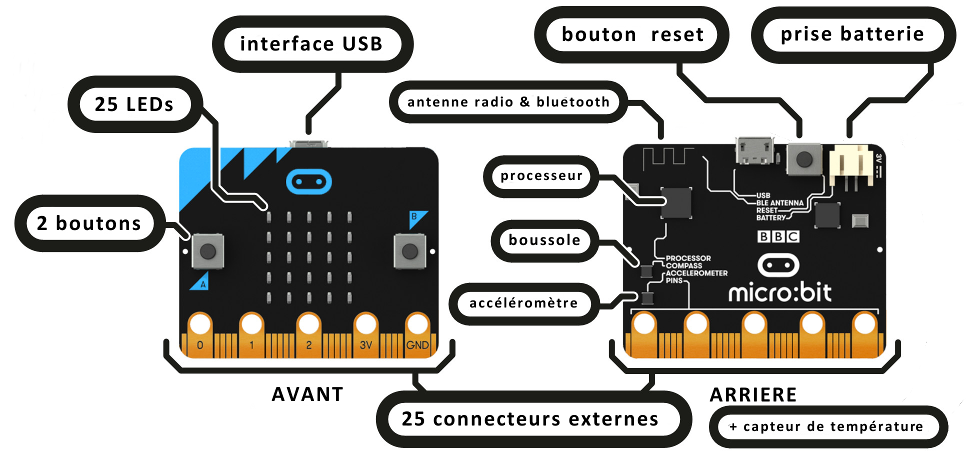
\includegraphics[width=0.95\linewidth]{images/microbit-hardware-access-fr.png}\end{center}

On utilise l'IDE Mu qui permet facilement de flasher la carte, et la bibliothèque dédiée :

\begin{minted}{python3}
from microbit import *
\end{minted}

On pourra trouver une introduction et des précisions sur le langage MicroPython utilisé :

\href{https://microbit-micropython.readthedocs.io/fr/latest/tutorials/introduction.html}{https://microbit-micropython.readthedocs.io/fr/latest/tutorials/introduction.html}

\section{Capteurs et actionneurs}

\Cours{{\bfseries Capteur}

Un capteur est un périphérique d'entrée. Il permet l'acquisition d'une grandeur physique (température, luminosité, présence, distance, \ldots), qu'il transforme en un signal électrique (logique, analogique ou numérique) qui pourra être traité par le reste du système.
}

Par exemple, avec la micro\string:bit :

\begin{itemize}
	\item Deux boutons \pythoninline{button_a} et \pythoninline{button_b} de méthodes :
	
	\begin{tabular}{ll}
	\pythoninline{is_pressed()} & renvoie \pythoninline{True} ou \pythoninline{False} selon si le bouton A est enfoncé,  \\
	\pythoninline{was_pressed()} & renvoie \pythoninline{True} ou \pythoninline{False} selon si le bouton A a été appuyé et relâché, \\
	\pythoninline{get_presses()} & renvoie et remet à zéro le nombre de fois où A a été appuyé. \\
	\end{tabular}
    \item Un accéléromètre \pythoninline{accelerometer} de méthodes :

	\begin{tabular}{ll}
	\pythoninline{get_x()} & renvoie un entier relatif indiquant la direction selon l'axe (Ox),  \\
	\pythoninline{get_y()} & renvoie un entier relatif indiquant la direction selon l'axe (Oy), \\
	\pythoninline{get_z()} & renvoie un entier relatif indiquant la direction selon l'axe (Oz), \\
	\pythoninline{get_values()} & renvoie un triplet d'entiers relatifs indiquant la direction (x,y,z),  \\
	\pythoninline{current_gesture()} & renvoie le nom du geste en cours.  \\
	\end{tabular}
	
	MicroPython comprend les gestes :  \pythoninline{"up"}, \pythoninline{"down"}, \pythoninline{"left"}, \pythoninline{"right"}, 
	
	\pythoninline{"face up"}, \pythoninline{"face down"}, \pythoninline{"freefall"}, \pythoninline{"3g"}, \pythoninline{"6g"}, \pythoninline{"8g"}, \pythoninline{"shake"}.
	
	
    \item Une boussole \pythoninline{compass} de méthodes :
    \pythoninline{calibrate()} (indispensable en début d'utilisation), \pythoninline{is_calibrated()} et \pythoninline{clear_calibration()}.
    
    \pythoninline{get_x()}, \pythoninline{get_y()}, \pythoninline{get_z()} comme pour l'accéléromètre.
    
    \pythoninline{heading()} qui renvoie un angle entier positif en degrés (0 pour le nord à 360).
    
    \pythoninline{get_field_strength()} qui renvoie un entier représentant l'intensité magnétique.
    \item Un capteur de température, donnée par \pythoninline{temperature()}.
\end{itemize}

\Cours{{\bfseries Actionneur}

Un actionneur est un périphérique de sortie. Il permet la conversion de l'énergie (électrique) en une action physique (mécanique, lumineuse, \ldots).
}

La micro\string:bit seule ne possède qu'un actionneur : une grille de LED 5$\times$5 : \pythoninline{display}.

Ses méthodes principales :

\begin{itemize}
	\item \pythoninline{get_pixel(x, y)} renvoie un entier entre 0 et 9 d'intensité lumineuse,
	\item \pythoninline{set_pixel(x, y, valeur)} règle l'intensité lumineuse par une valeur entre 0 et 9,
	\item \pythoninline{clear()} règle toutes les intensités lumineuses à 0,
	\item \pythoninline{show(value, delay=400, wait=True, loop=False, clear=False)} :
	 
	\pythoninline{value} peut être un nombre, une chaine  de caractères, une image ou une liste d'images.
	
	Une image pouvant être l'une des images prédéfinies, \pythoninline{Image.HEART}, \pythoninline{Image.HEART_SMALL}, \pythoninline{Image.HAPPY}, \pythoninline{Image.SMILE}, \pythoninline{Image.SAD} \ldots ou créée en indiquant l'intensité lumineuse de chaque LED (de gauche à droite et de haut en bas) :
	
    \pythoninline{image = Image("90009:09090:00900:09090:90009")}.
	
	\pythoninline{delay} est le temps en microsecondes entre deux images d'une liste.
	
	\pythoninline{wait} bloque l'exécution si \pythoninline{True}, affiche en tache de fond si \pythoninline{False}.
	
	\pythoninline{loop} détermine s'il y a répétition ou non.
	
	\pythoninline{clear} détermine si l'affichage est effacé après l'exécution. 
	\item \pythoninline{scroll(value, delay=150, wait=True, loop=False, monospace=False)}.
	
\end{itemize}

\section{Réalisation d'une Interface Homme Machine}

Si l'on veut faire se déplacer un point lumineux selon l'inclinaison de la carte et terminer en fixant sa position, on a besoin de :

\begin{itemize}
	\item initialiser la position. Par exemple au centre : \pythoninline{x = 3} et \pythoninline{y = 3}.
	\item utiliser une boucle qui ne s'arrête que si l'utilisateur le demande par une action,
	      
	       Par exemple : \pythoninline{while not button_a.is_pressed() :}
	\item lire les données du bon capteur.
	
	Ici : \pythoninline{accelerometer.get_x()} et \pythoninline{accelerometer.get_y()}.
	
	\item utiliser ces données pour mettre à jour les variables du programme.
	
	\item agir sur le bon actionneur en fonction de cette mise à jour.
	
	Ici : \pythoninline{display.set_pixel(int(x),int(y),9)} 
	
\end{itemize}

Ce qui donne finalement :

\begin{minted}{python}
from microbit import *

x = 3
y = 3
while not button_a.is_pressed() :
    x = x + accelerometer.get_x() / 1000
    y = y + accelerometer.get_y() / 1000
    if(x>4): x = 4
    if(x<0): x = 0
    if(y>4): y = 4
    if(y<0): y = 0
    sleep(100)
    display.clear()
    display.set_pixel(int(x),int(y),9)
\end{minted}













%(robot : Micro\string:Maqueen ? )

\partie{Langages et programmation}
\chapter*{Programme officiel}

\section*{Programme officiel}

Les langages de programmation Turing-complets sont caractérisés par un corpus de « cons-tructions élémentaires ». Sans introduire cette terminologie, il s'agit de montrer qu'il existe de nombreux langages de programmation, différents par leur style (impératif, fonctionnel, objet, logique, événementiel, etc.), ainsi que des langages formalisés de description ou de requêtes qui ne sont pas des langages de programmation.

L'importance de la spécification, de la documentation et des tests est à présenter, ainsi que l'intérêt de la modularisation qui permet la réutilisation de programmes et la mise à disposition de bibliothèques. Pour les programmes simples écrits par les élèves, on peut se contenter d'une spécification rapide mais précise.

{\centering\begin{tabular}{|L{3cm}|L{5.5cm}|L{6cm}|}\hline
\cellcolor{bo}\bfseries\textcolor{white}{Contenus}&
\cellcolor{bo}\bfseries\textcolor{white}{Capacités attendues}&
\cellcolor{bo}\bfseries\textcolor{white}{Commentaires}\\ \hline
Constructions élémentaires
&
Mettre en évidence un corpus de constructions élémentaires.
& Séquences, affectation, conditionnelles, boucles bornées, boucles non bornées, appels de fonction.\\ \hline
Diversité et unité des langages de programmation
&
Repérer, dans un nouveau langage de programmation, les traits communs et les traits particuliers à ce langage.
&
Les manières dont un même programme simple s'écrit dans différents langages sont comparées.\\ \hline
Spécification
&
Prototyper une fonction.

Décrire les préconditions sur les arguments.

Décrire des postconditions sur les résultats.
&
Des assertions peuvent être utilisées pour garantir des préconditions ou des postconditions.\\ \hline
Mise au point de programmes
&
Utiliser des jeux de tests.
&
L'importance de la qualité et du nombre des tests est mise en évidence.

Le succès d'un jeu de tests ne garantit pas la correction d'un programme.\\ \hline
Utilisation de bibliothèques
&
Utiliser la documentation d'une bibliothèque.
&
Aucune connaissance exhaustive d'une bibliothèque particulière n'est exigible.\\ \hline
\end{tabular}\par}


\chapter{Constructions élémentaires}

Cette partie est volontairement non détaillée pour tenir sur une page de référence. Ces notions ont déjà été rencontrées en particulier en mathématiques avant l'entrée en Première.

\begin{multicols}{2}

{\bfseries Valeurs}

\begin{itemize}
	\item \pythoninline{1} est de type \pythoninline{int}
	\item \pythoninline{1.0} est de type \pythoninline{float}
	\item \pythoninline{True} est de type \pythoninline{bool}
	\item \pythoninline{'1'} est de type \pythoninline{str}
	\item \pythoninline{[1, 2]} est de type \pythoninline{list}
	\item \pythoninline{(1, 2)} est de type \pythoninline{tuple}
	\item \pythoninline{{'un' : 1, 'deux' : 2}}  de type \pythoninline{dict}
\end{itemize}

\medskip
{\bfseries Variables}

L'affectation \fbox{$x\leftarrow 1$} : \pythoninline{x = 1}.


\medskip
{\bfseries Conditionnelle}

\begin{algorithm}[H]
$x \leftarrow 96$\;
\lSi{$x$ est pair}{$x \leftarrow \frac{x}{2}$}
\end{algorithm}

\vspace{-1ex}
\begin{minted}{python}
x = 96
if x % 2 == 2 :
    x = x // 2
\end{minted}

\begin{algorithm}[H]
$x \leftarrow 96$\;
\lSi{$x$ est pair}{$x \leftarrow \frac{x}{2}$}
\lSinon{$x \leftarrow x * 3 + 1$}
\end{algorithm}

\vspace{-1ex}
\begin{minted}{python}
x = 96
if x % 2 == 2 :
    x = x // 2
else :
    x = x * 3 + 1
\end{minted}

\begin{algorithm}[H]
$x \leftarrow $ entier aléatoire entre -5 et 5\;
\lSi{$x>0$}{ $x \leftarrow x + 1$ }
\lSinonSi{$x<0$}{$x \leftarrow x - 1$}
\lSinon{$x \leftarrow 1$ ou $-1$ au hasard}
\end{algorithm}

\vspace{-1ex}
\begin{minted}{python}
from random import randint

x = randint(-5,5)
if x > 0 :
    x = x + 1
elif x < 0 :
    x = x - 1
else :
    x = 1 - 2 * randint(0,1)
\end{minted}



\medskip
{\bfseries Boucle non bornée}

\begin{algorithm}[H]
$x \leftarrow 96$\;
\Tq {$x$ est pair}
{   
    $x \leftarrow \frac{x}{2}$\;
}
\end{algorithm}

\vspace{-1ex}
\begin{minted}{python}
x = 96
while x % 2 == 0 :
    x = x // 2
\end{minted}


\medskip
{\bfseries Boucle bornée}

\begin{algorithm}[H]
\Pour{$k$ {\normalfont\bfseries allant de} $0$ {\normalfont\bfseries à} $9$}
{ affiche($k$)\; }
\end{algorithm}

\vspace{-1ex}
\begin{minted}{python}
for k in range (10) :
    print(k)
\end{minted}

\begin{itemize}
	\item \pythoninline{range(n)} de $0$ à $n-1$
	\item \pythoninline{range(d,n)} de $d$ à $n-1$
	\item \pythoninline{range(d,n,p)} de $d$ à $n-1$ de $p$ en $p$
\end{itemize}

Avec $d$, $n$ et $p$ entiers.

Peut aussi être utilisé directement sur les types \pythoninline{str}, \pythoninline{list}, \pythoninline{tuple} et \pythoninline{dict}.


\medskip
{\bfseries Fonction}


\begin{minted}{python}
def f(x) :
    x = x * 2
    return x

x = 3
y = f(x)
print('f(',x,') = ',y, sep = '')
\end{minted}

La variable \pythoninline{x} de la fonction est dite locale. Elle copie la référence obtenue par le paramètre. Changer sa valeur ne change donc pas celle de la variable \pythoninline{x} externe à la fonction.

Pour un type construit (un tableau), cette référence donne accès aux éléments qui, si modifiés, le sont alors de manière globale.

\end{multicols}

\chapter{Différents langages}

En introduction, voici quelques façons de produire dans différents langages, l'affichage des mots << Hello, world ! >>, à commencer par Python :

\vspace{-2ex}
\begin{minted}{python}
print('Hello, world!')
\end{minted}

\begin{multicols}{2}
Langage Bash :

\vspace{-2ex}
\begin{minted}{bash}
#!/bin/bash
echo 'Hello, world!'
\end{minted}

Langage C :

\vspace{-2ex}
\begin{minted}{C}
#include <stdio.h>

int main()
{
    printf("hello, world");
    return 0;
}
\end{minted}

Langage HTML5 :

\vspace{-2ex}
\begin{minted}{html}
<!DOCTYPE html>
<html>
    <head>
        <meta charset="utf-8">
        <title>Hello, world!</title>
    </head>
    <body>
        <p>Hello, world!</p>
    </body>
</html>
\end{minted}

Langage Java :

\vspace{-2ex}
\begin{minted}[fontsize = \footnotesize]{java}
public class HelloWorld {
    public static void main(String[] args) {
        System.out.println("Hello, world!"); 
    }
}
\end{minted}

Langage JavaScript :

\vspace{-2ex}
\begin{minted}{js}
console.log("Hello, world!");
\end{minted}

Langage \LaTeX (utilisé pour ce document) :

\vspace{-2ex}
\begin{minted}{latex}
\documentclass{minimal}
\begin{document}
Hello, world!
\end{document}
\end{minted}

Langage PHP :

\vspace{-2ex}
\begin{minted}{php}
<?php
 echo "Hello, world!";
?>
\end{minted}
\end{multicols}

À première vue, ils semblent très différents, mais le plus important est qu'ils peuvent tous faire une même chose : produire un affichage de texte !
\medskip

HTML et LATEX sont deux langages à balises de définition de documents. On peut identifier \mintinline{html}{<html>...</html>} et  \mintinline{html}{\begin{document}...\end{document}}. L'un destine son résultat à l'écran et l'autre à l'impression, mais ils sont très comparables.
  
\medskip

Python, C, Java, ... sont des langages de programmation impératifs. On y retrouve
\begin{itemize}
  \item des séquences d'instructions, séparées par un simple passage à la ligne pour Python, par un point-virgule \mintinline{C}{;} dans beaucoup d'autres langages ;
  
  \item des affectations, \mintinline{C}{x = 3} en Python, C, Java, JavaScript... ; \mintinline{C}{$x = 3} en PHP ; %$
  
  ( \mintinline{C}{x := 3}, \mintinline[escapeinside=||]{C}{x |$\leftarrow$| 3} ou encore  \mintinline[escapeinside=||]{C}{3 |$\rightarrow$| x} ... dans d'autres langages. )
  
  \item des instructions conditionnelles :

\begin{multicols}{2}  
  en Python :
  
  
  \vspace{-2ex}
\begin{minted}{python3}
if (x == 3) :
    print("Ok")
\end{minted}
  
  
   en JavaScript :
  
  \vspace{-2ex}
\begin{minted}{javascript}
if (x == 3) {
    console.log("Ok");
}
\end{minted}
  \end{multicols}

Dans beaucoup de langages, les blocs d'instructions  sont délimités par des accolades  \mintinline{C}{{ ... }}, quand, en Python, ils commencent après \mintinline{python3}{:} et sont identifiés par une indentation.
  
  \item des boucles :

\begin{multicols}{2}  
  boucle \texttt{pour} en Python :
  
  
  \vspace{-2ex}
\begin{minted}{python3}
chiffres = ""
for i in range(10) :
    chiffres = chiffres + i
\end{minted}
  
  
   en JavaScript :
  
  \vspace{-2ex}
\begin{minted}{javascript}
var chiffres = "";
for (var i = 0; i < 10; i++) {
  chiffres = chiffres + i;
}
\end{minted}
\end{multicols}

En JavaScript la boucle \texttt{pour} est définie par une initialisation, une condition à vérifier pour continuer et une instruction à exécuter en fin de boucle. (Une autre syntaxe, proche de celle de Python existe en JavaScript). Certains langages sont plus proches du \texttt{pour} algorithmique.


La boucle \texttt{while} est semblable pour les langages proposés ici. On remplace \mintinline{python3}{if} par \mintinline{python3}{while} pour répéter le bloc conditionnel.
  
  \item des branchements.
  
  Il s'agit de possibilités de sauter d'une partie du programme à une autre. En particulier l'appel à une fonction.
  
  

\begin{multicols}{2}  
  Fonction en Python :
  
  
  \vspace{-2ex}
\begin{minted}{python3}
def f(x) :
    return x * x 
\end{minted}
  
  
   En JavaScript :
  
  \vspace{-2ex}
\begin{minted}{javascript}
function f(x) {
  return x * x;
}
\end{minted}


  
  
   En C :
  
  \vspace{-2ex}
\begin{minted}{c}
int f(int x)
{
    return x * x;
}
\end{minted}

Et l'appel (commun à ces langages)

\pythoninline{f(7)} renvoie 49.

\end{multicols}
  
  
  
\end{itemize} 

\medskip

Il existe d'autres types de programmation qui pourront être discutés en Terminale.


\chapter{Spécification et tests}

\section{Prototype d'une fonction}

\Cours{{\bfseries Prototype} 

Le prototype d'une fonction est sa \emph{signature}. Il définit : 

\begin{itemize}
	\item le nom de la fonction,
	\item le nombre et le type de ses paramètres,
	\item le type de la valeur qu'elle renvoie.
\end{itemize}
}

Avec les langages C ou Java par exemple, on écrit le prototype des fonctions. Cela permet par exemple d'écrire la partie principale en début de code contrairement au langage Python. La commande \pythoninline{def} définit la fonction en place ; elle n'a aucune existence pour le code la précédant.

\begin{multicols}{2}  
  Fonction en Python :
  
  (Pas de prototype)
  
  \vspace{-2ex}
\begin{minted}{python3}
def f(x) :  # Définition en place
    return x * x 
\end{minted} 
  
   En C :
  
  \vspace{-2ex}
\begin{minted}{c}
int f(int x)  // Prototype
{
    return x * x;
}
\end{minted}
\end{multicols}

Un des avantages d'une fonction sans prototype est qu'elle peut éventuellement être utilisée avec des valeurs de types différents : \pythoninline{f(3.5)} sera évalué correctement en Python, mais sera refusé par le compilateur C qui attend un argument entier.

Un des inconvénients est qu'on perd en lisibilité sur l'intention de la fonction. C'est pourquoi il est important de commenter son code, en particulier chaque fonction pour préciser sa spécification.

\section{Spécification}

\Cours{{\bfseries Spécification} 

La spécification d'un algorithme (et donc d'une fonction) définit :
  
  \vspace{-2ex}
\begin{multicols}{2}
\begin{itemize}
	\item les entrées et sorties
	\item le rôle
	\item les préconditions
	\item les postconditions
\end{itemize}
\end{multicols}
}
\begin{itemize}
	\item Les entrées et sorties sont ce qui fait le prototype d'une fonction.

	\item Le rôle est une description du problème que résout l'algorithme (la fonction).

	\item Les préconditions sont des précisions sur la nature exacte des entrées.

	\item Les postconditions sont des précisions sur la nature exacte des sorties.
\end{itemize}


Les préconisations sont les hypothèses (au sens mathématique) sur les entrées, permettant de démontrer que l'algorithme (ou la fonction) joue bien son rôle, c'est à dire produit des sorties vérifiant les postconditions.

\medskip

Avec le langage Python on écrit la spécification avec le code dans des \emph{docstring}. C'est un texte entouré de guillemets triples qui se place juste en début de code :

  
  \vspace{-2ex}
\begin{minted}{python3}
def f(x):
    """Renvoie le carré du nombre donné en argument."""
    return x * x
\end{minted}

Pour un algorithme simple comme celui-ci, une seule ligne précisant son rôle peut suffire. Mais il n'est pas rare que le \emph{docstring} soit plus long que le code lui-même :

  
  \vspace{-2ex}
\begin{minted}{python3}
def centSur(x):
    """Calcule le quotient entier de 100 par x.
    
    Cette fonction opère la division entière de 100 par x et en
    renvoie le quotient.
    
    :param x: Un entier non nul.
    :type x: int
    :return: Le quotient de la division entière de 100 par x
    :rtype: int
    """
    return 100 // x
\end{minted}

Cette exemple utilise la syntaxe RST mais ce n'est pas une obligation. 
 
 On obtient alors l'affichage de cette documentation avec la commande \pythoninline{help(centSur)}.

\section{Tests et assertions}

Un \emph{docstring} permet de documenter en écrivant la spécification des fonctions. Il permet aussi la mise au point des programmes à l'aide de jeux de tests. En effet, juste après la spécification, et avant même de réfléchir à l'algorithme, on peut mettre en place un jeu de tests qu'il devrait passer pour avoir une chance de résoudre le problème posé.

\begin{minted}{python3}
def centSur(x):
    """Calcule le quotient entier de 100 par x.
    
    >>> centSur(3)
    33
    """
    return 100 // x
\end{minted}

La bibliothèque \pythoninline{doctest} permet effectivement de lancer tous les tests par la commande \pythoninline{doctest.testmod()}. Pour voir tous les tests effectués, on peut compléter cette commande  en \pythoninline{doctest.testmod(verbose = True)}.

 La réussite à ces tests n'est pas une preuve de correction, mais permet de guider la programmation et l'utilisateur.
 
 \medskip
 
 En phase de conception ou plutôt de débogage, on peut vouloir s'assurer que les préconditions sont effectivement remplies. Dans ce cas, on utilise des assertions : on exprime chacune des préconditions après le mot clef \pythoninline{assert}. 
 
\begin{minted}{python3}
def centSur(x):
    """Calcule le quotient entier de 100 par x."""
    assert isinstance(x, int)
    assert x != 0
    return 100 // x
\end{minted}

Avec ce code, par exemple, \pythoninline{centSur(5.0)} provoquera une erreur, alors que sans la première assertion, il aurait donné une réponse.

\chapter{Utilisation de bibliothèques}

\Cours{{\bfseries Bibliothèque}

Une bibliothèque, on dit souvent un \emph{module} en Python, est un fichier contenant un ensemble de fonctions, de classes (types personnalisés), et de constantes, que l'on peut importer dans son propre programme pour les utiliser.
}

\section{Utilisation de modules existants}

Il existe de très nombreux modules en Python (c'est un des avantages de ce langage). Certains sont dits \emph{standards} et fournis avec l'installation du langage. D'autres doivent être installés manuellement.

Parmi les standards, notons :

\begin{itemize}
	\item \pythoninline{random} dont la fonction \pythoninline{randint()} permet d'obtenir un entier aléatoire dans un intervalle,
	\item \pythoninline{math} qui contient par exemple \pythoninline{cos()} et \pythoninline{sin()},
	\item \pythoninline{doctest} pour implémenter des tests automatiques de fonctions,
	\item \pythoninline{csv} pour le traitement de tables CSV,
	\item \pythoninline{json} pour le traitement de données JSON,
	\item \pythoninline{socket} pour les connexions TCP/IP,
	\item \pythoninline{os} et \pythoninline{sys} pour les fonctions système.
\end{itemize}

Parmi les autres, on peut citer :

\begin{itemize}
	\item \pythoninline{PIL} pour le traitement d'images (à charger sous le nom \pythoninline{pillow}),
	\item \pythoninline{requests} pour les requêtes HTTP GET et POST,
	\item \pythoninline{http.server} pour un serveur HTTP (réponse aux GET et POST).
\end{itemize}

\medskip

Pour utiliser une bibliothèque déjà installée, on peut employer une des méthodes suivantes :

\begin{multicols}{2}
\begin{minted}{python3}
import random

x = random.randint(1,9)
\end{minted}

\begin{minted}{python3}
import random as hasard

x = hasard.randint(1,9)
\end{minted}

\begin{minted}{python3}
from random import randint

x = randint(1,9)
\end{minted}

\begin{minted}{python3}
from random import randint as hasard

x = hasard(1,9)
\end{minted}
\end{multicols}

\medskip

Pour une bibliothèque non standard, il faut passer en ligne de commande pour la charger et l'installer avec le module \pythoninline{pip}. Par exemple pour \pythoninline{PIL} :

\noindent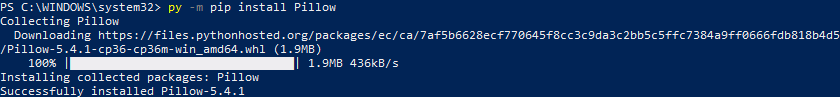
\includegraphics[width=\textwidth]{images/installPillow.png}

\section{Conception de modules}

N'importe quel fichier Python est un module dont le nom est celui du fichier. Il est donc très simple d'en concevoir un :

\begin{multicols}{2}
Fichier \texttt{Bonjour.py} :

\vspace{-2ex}
\begin{minted}{python3}
""" Ceci est le module Bonjour """

def hello():
    """ Affiche : Bonjour ! """
    print('Bonjour !')

hello()
\end{minted}

Script dans le même répertoire :

\begin{minted}{python3}
import Bonjour

Bonjour.hello()
\end{minted}

Ce second script s'exécute bien...

Mais dit bonjour deux fois !
\end{multicols}

Au moment de l'importation, le script contenu dans le module est entièrement exécuté. Comme il contient un appel à la fonction \pythoninline{hello()}, on obtient un premier affichage, puis un second dû à l'appel \pythoninline{Bonjour.hello()} du second script.

On pourrait enlever le \pythoninline{hello()} du module, mais dans la pratique, on souhaite souvent garder à un module la possibilité de s'exécuter en tant que script principal. Il suffit pour cela d'ajouter une conditionnelle :

\begin{multicols}{2}
\begin{minted}{python3}
""" Ceci est le module Bonjour """

def hello():
    """ Affiche bonjour """
    print('Bonjour !')
    
if __name__ == "__main__":
    hello()
\end{minted}

Par exemple, en phase de développement, on pourra utiliser :

\begin{minted}{python3}
if __name__ == '__main__':
   import doctest
   doctest.testmod()
\end{minted}
\end{multicols}

Si on prend l'exemple proposé pour l'explication sur les assertions, on obtient :

\begin{minted}{python3}
""" Module de test sur les assertions """

def centSur(x):
    """Calcule le quotient entier de 100 par x.
    
    Cette fonction opère la division entière de 100 par x et en
    renvoie le quotient.    
    
    :param x: Un entier non nul
    :type x: int
    :return: Le quotient de la division entière de 100 par x
    :rtype: int
    
    >>> centSur(3)
    33
    
    >>> centSur(3.0)
    Traceback (most recent call last):
        ...
    AssertionError: x doit être entier
    
    >>> centSur(0)
    Traceback (most recent call last):
        ...
    AssertionError: x ne doit pas être nul
    """
    assert isinstance(x, int), 'x doit être entier'
    assert x != 0, 'x ne doit pas être nul'
    return 100 // x

if __name__ == '__main__':
    import doctest
    doctest.testmod(verbose=True)
\end{minted}

\partie{Algorithmique}
\chapter*{Programme officiel}

\section*{Programme officiel}

Le concept de méthode algorithmique est introduit ; de nouveaux exemples seront vus en terminale. Quelques algorithmes classiques sont étudiés. L'étude de leurs coûts respectifs prend tout son sens dans le cas de données nombreuses, qui peuvent être préférentiellement des données ouvertes.

Il est nécessaire de montrer l'intérêt de prouver la correction d'un algorithme pour lequel on dispose d'une spécification précise, notamment en mobilisant la notion d'invariant sur des exemples simples. La nécessité de prouver la terminaison d'un programme est mise en évidence dès qu'on utilise une boucle non bornée (ou, en terminale, des fonctions récursives) grâce à la mobilisation de la notion de variant sur des exemples simples.

{\centering\begin{tabular}{|L{3cm}|L{5.5cm}|L{6cm}|}\hline
\cellcolor{bo}\bfseries\textcolor{white}{Contenus}&
\cellcolor{bo}\bfseries\textcolor{white}{Capacités attendues}&
\cellcolor{bo}\bfseries\textcolor{white}{Commentaires}\\ \hline
Parcours séquentiel d'un tableau
&
Écrire un algorithme de recherche d'une occurrence sur des valeurs de type quelconque.

Écrire un algorithme de recherche d'un extremum, de calcul d'une moyenne.
&
On montre que le coût est linéaire.\\ \hline
Tris par insertion, par sélection
&
Écrire un algorithme de tri.

Décrire un invariant de boucle qui prouve la correction des tris par insertion, par sélection.
&
La terminaison de ces algorithmes est à justifier.

On montre que leur coût est quadratique dans le pire cas.\\ \hline
Algorithme des k plus proches voisins
&
Écrire un algorithme qui prédit la classe d'un élément en fonction de la classe majoritaire de ses k plus proches voisins.
&
Il s'agit d'un exemple d'algorithme d'apprentissage.\\ \hline
Recherche dichotomique dans un tableau trié
&
Montrer la terminaison de la recherche dichotomique à l'aide d'un variant de boucle.
&
Des assertions peuvent être utilisées.

La preuve de la correction peut être présentée par le professeur.\\ \hline
Algorithmes gloutons
&
Résoudre un problème grâce à un algorithme glouton.
&
Exemples : problèmes du sac à dos ou du rendu de monnaie.

Les algorithmes gloutons constituent une méthode algorithmique parmi d'autres qui seront vues en terminale.\\ \hline
\end{tabular}\par}


\chapter{Recherches dans un tableau}
\newcommand{\carte}[2][white]{%
\newcount\cou%
\newcount\val%
\val=#2%
\cou=#2%
\advance\cou by-1%
\divide\cou by13%
\def\couleur{$\spadesuit$}\def\couleurtexte{black}%
\ifnum\cou=1\def\couleur{$\color{rouge}\heartsuit$}\def\couleurtexte{rouge}\fi%
\ifnum\cou=2\def\couleur{$\color{rouge}\diamondsuit$}\def\couleurtexte{rouge}\fi%
\ifnum\cou=3\def\couleur{$\clubsuit$}\fi%
\multiply\cou by-13%
\advance\val by\cou%
\def\valeur{\the\val}%
\ifnum\val=11\def\valeur{V}\fi%
\ifnum\val=12\def\valeur{D}\fi%
\ifnum\val=13\def\valeur{R}\fi%
\def\dessin{\tiny\begin{tabular}{@{}c@{}}\color{\couleurtexte}\valeur\\\couleur\end{tabular}}%
\begin{tikzpicture}%
\draw[fill=#1,rounded corners=1.5pt](0,0)rectangle(1,1.5);%
\node[below right=1pt,xscale=0.75,inner sep = 0]at(0,1.5){\dessin};%
\node[below left=1pt,xscale=0.75,inner sep = 0]at(1,1.5){\dessin};%
\node[above right=1pt,xscale=0.75,inner sep = 0]at(0,0){\rotatebox{180}{\dessin}};%
\node[above left=1pt,xscale=0.75,inner sep = 0]at(1,0){\rotatebox{180}{\dessin}};%
\node[yscale=2,xscale=1.5]at(0.5,0.75){\dessin};%
\end{tikzpicture}}

\begin{center} Comment trouver une information parmi beaucoup d'autres ?

\begin{tikzpicture}
\foreach \v in {0.02,0.04,...,2.6}
\fill[opacity=0.002](4,2)ellipse(2*\v cm and \v cm);
\foreach \v/\x/\y/\a in {10	/	1.23	/	1.05	/	256	,
32	/	2.49	/	0.59	/	46	,
41	/	3.00	/	3.94	/	296	,
40	/	4.07	/	0.96	/	334	,
42	/	1.14	/	2.93	/	283	,
46	/	3.69	/	3.01	/	336	,
43	/	2.78	/	1.07	/	157	,
4	/	6.55	/	3.98	/	115	,
49	/	7.66	/	1.28	/	85	,
5	/	4.26	/	2.32	/	311	,
12	/	4.24	/	2.39	/	355	,
48	/	4.67	/	2.69	/	171	,
25	/	5.70	/	2.17	/	156	,
26	/	4.01	/	2.33	/	98	,
38	/	3.51	/	2.04	/	235	,
31	/	4.86	/	3.61	/	322	,
52	/	0.94	/	1.29	/	79	,
45	/	5.49	/	2.29	/	158	,
7	/	3.71	/	0.43	/	202	,
13	/	1.62	/	0.95	/	334	,
44	/	7.33	/	0.85	/	229	,
21	/	7.30	/	2.05	/	140	,
9	/	1.47	/	1.15	/	182	,
34	/	7.19	/	1.46	/	266	,
11	/	0.62	/	0.65	/	11	,
17	/	2.09	/	0.02	/	234	,
16	/	4.70	/	0.09	/	187	,
50	/	7.31	/	3.84	/	302	,
23	/	7.29	/	2.69	/	75	,
28	/	7.89	/	3.57	/	343	,
37	/	0.83	/	2.06	/	346	,
51	/	2.71	/	2.14	/	250	,
36	/	6.34	/	2.62	/	183	,
24	/	0.94	/	1.84	/	59	,
27	/	3.76	/	3.50	/	53	,
20	/	3.25	/	3.02	/	17	,
15	/	6.14	/	3.85	/	50	,
8	/	1.80	/	0.42	/	185	,
39	/	3.50	/	1.06	/	151	,
29	/	6.12	/	0.76	/	116	,
47	/	6.30	/	1.58	/	296	,
30	/	4.88	/	0.19	/	304	,
33	/	5.09	/	3.27	/	283	,
19	/	2.59	/	0.49	/	71	,
6	/	5.64	/	2.80	/	156	,
14	/	5.40	/	2.95	/	47	,
1	/	7.56	/	2.71	/	343	,
18	/	0.46	/	2.49	/	41	,
3	/	7.85	/	1.85	/	293	,
22	/	1.54	/	3.46	/	34	,
35	/	0.86	/	2.21	/	279	,
2	/	4.44	/	0.82	/	137	
} \node[rotate=\a]at(\x*1cm,\y*1cm){\carte{\v}};
\end{tikzpicture}\end{center}

Une solution élémentaire est de faire un tas et de passer en revue toutes les cartes une à une.

\section{Parcours séquentiel d'un tableau}

Pour simplifier l'exemple, supposons que l'on ait tiré une main et notons les valeurs des cartes dans un tableau :

\begin{center}
\begin{tikzpicture}[baseline={([yshift=-.5ex]current bounding box.center)}]
\foreach \v/\a in {25/50,1/40,33/30,52/20,29/10,31/0,24/-10,28/-20,5/-30,34/-40} 
  \draw[shift={(90+\a:0.75)},color=black]node[rotate=\a]{\carte{\v}};
\end{tikzpicture}
\begin{minipage}{8.5cm}
\begin{tabular}{|c|c|c|c|c|c|c|c|c|c|}
\hline
\small DC &\small 1P &\small 7c &\small RT &\small 3c &\small 5c&\small VC&\small 2c&\small 5P&\small 8c\\
\hline
\end{tabular}
\end{minipage}

\pythoninline{ cartes = ['DC', '1P', '7c', 'RT', '3c', '5c', 'VC', '2c', '5P', '8c']}
\end{center}

\subsection{Spécification possible}

\begin{itemize}
	\item {\bfseries Entrée :} Tableau $T$ de longueur $n$, et une valeur $v$.
	\item {\bfseries Sortie :} Un indice $i$ de $v$ dans $T$ ou $-1$ si $v$ n'est pas dans $T$. 
	\item {\bfseries Rôle :} Recherche d'une occurrence de $v$ dans $T$.
	\item {\bfseries Précondition :} $v$ est comparable avec les éléments de $T$.
	\item {\bfseries Postcondition :} ($i=-1$ et $v$ n'est pas dans $T$) ou ($0\leqslant i < n$ et $T[i]$ est $v$).
\end{itemize}

\subsection{Algorithme}

\begin{algorithm}[H]
$i \leftarrow -1$\;
\Pour{$carte$ {\normalfont\bfseries allant de} $0$ {\normalfont\bfseries à} $n-1$}
{ \Si{$\text{\normalfont T}[carte]==v$}
  {  $i\leftarrow carte$\;  }
}
\end{algorithm}

\subsection{Correction et complexité}

\begin{itemize}
	\item {\bfseries Correction partielle :} On peut prendre comme invariant, pour la boucle \texttt{pour}, la postcondition limitée au sous-tableau déjà parcouru.
	
	Invariant : ($i=-1$ et si $0\leqslant j\leqslant carte$ alors $\text{\normalfont T}[j]\ne v$) ou ($0\leqslant i \leqslant carte$ et $\text{\normalfont T}[i]=v$).
	
	Avant la première itération $carte$ n'est pas définie et on a bien $i=-1$.
	
	Après la première itération $carte=0$ ; si la condition $\text{\normalfont T}[carte]==v$ a été vérifiée, alors on a $0= i = carte$ donc $0\leqslant i \leqslant carte$ et $\text{\normalfont T}[i]=v$ ; sinon, on a toujours $ i = -1$ et pour $0\leqslant j\leqslant carte$ c'est à dire $j=0$, on a aussi  $\text{\normalfont T}[j]\ne v$. L'invariant est donc vérifié.
	
	S'il est vérifié avant une itération, alors on peut distinguer 4 cas :
	\begin{itemize}
		\item ($i=-1$ et si $0\leqslant j\leqslant carte$ alors $\text{\normalfont T}[j]\ne v$) et la conditionnelle se réalise ;
		\item ($i=-1$ et si $0\leqslant j\leqslant carte$ alors $\text{\normalfont T}[j]\ne v$) et la conditionnelle ne se réalise pas ;
		\item ($0\leqslant i \leqslant carte$ et $\text{\normalfont T}[i]=v$)  et la conditionnelle se réalise ;
		\item ($0\leqslant i \leqslant carte$ et $\text{\normalfont T}[i]=v$)  et la conditionnelle ne se réalise pas.
	\end{itemize}
	
	Dans chaque cas, on peut vérifier comme précédemment que l'invariant est bien conservé.
	
	Enfin, l'expression de l'invariant après la dernière itération donne la postcondition.
	\item {\bfseries Terminaison :} Une boucle \texttt{pour} termine.
	\item {\bfseries Complexité :} La taille des entrées est la longueur $n$ du tableau.
	
	Le pire cas vient d'une réalisation systématique de la condition $\text{\normalfont T}[carte]=v$, c'est à dire un tableau dont toutes les valeurs sont égales à $v$.
	
	Dans ce cas, on peut compter 3 opérations par itération (mise à jour de $carte$, comparaison de la conditionnelle, et affectation de $i$). La boucle faisant $n$ itérations, on obtient en tout $3n+1$ opérations.
	
	$3n+1 = O(n)$. La complexité est linéaire.
\end{itemize}

\subsection{Applications}

Appliquons l'algorithme précédent à un tableau de nombres :

\pythoninline{tableau = [1, 5, 7, 3, 2, 9, 4, 6]}

\subsubsection{Recherche d'un maximum}

La valeur recherchée n'est pas connue, mais vérifie un critère. 

Ajoutons la {\bfseries précondition} suivante pour initialiser : $T$ n'est pas vide.

On peut alors adapter l'algorithme précédent :

\begin{algorithm}[H]
$max \leftarrow T[0]$\;
\Pour{$i$ {\normalfont\bfseries allant de} $0$ {\normalfont\bfseries à} $n-1$}
{ \Si{$\text{\normalfont T}[i]>max$}
  {  $max \leftarrow \text{\normalfont T}[i]$\;  }
}
\end{algorithm}

Une preuve similaire s'applique et la complexité est toujours linéaire.


\subsubsection{Calcul d'une moyenne}

Toutes les valeurs sont utilisées : l'algorithme est simplifié (plus de conditionnelle).

\begin{algorithm}[H]
$somme \leftarrow 0$\;
\Pour{$i$ {\normalfont\bfseries allant de} $0$ {\normalfont\bfseries à} $n-1$}
{ $somme \leftarrow somme + \text{\normalfont T}[i]$\;  }
$moyenne \leftarrow somme / n$\;
\end{algorithm}

Un invariant possible pour la correction partielle : $somme$ est la somme des valeurs de T d'indices inférieurs à $i$.

La complexité est toujours linéaire.


\section{Recherche dichotomique}

On rajoute ici une précondition importante : Le tableau est \emph{trié}.

On pourrait définir plusieurs critères (couleur / valeur / points dans un jeu ...). Dans ce qui suit, on supposera établi un ordre total qui permet la numérotation :

\begin{center}\begin{tikzpicture}
\foreach \v in {1,...,52} {
  \node at(\v*0.28cm,0cm){\carte{\v}};
  \node[scale=0.6,xshift=-0.7cm,yshift=-1.3cm,below]at(\v*0.28cm,0){\v};
 }
\end{tikzpicture}
\end{center}

On peut réécrire notre main :

\vspace{-3ex}
\begin{center}\begin{tikzpicture}[baseline={([yshift=-.5ex]current bounding box.center)}]
\foreach \v/\a in {25/50,1/40,33/30,52/20,29/10,31/0,24/-10,28/-20,5/-30,34/-40} 
  \draw[shift={(90+\a:0.75)},color=black]node[rotate=\a]{\carte{\v}};
\end{tikzpicture}
\begin{minipage}{8.5cm}
\begin{tabular}{|c|c|c|c|c|c|c|c|c|c|}
\hline
\small 25&\small 1&\small 33&\small 52&\small 29&\small 31&\small 24&\small 28&\small 5&\small 34\\
\hline
\end{tabular}
\medskip

\pythoninline{ cartes = [25,1,33,52,29,31,24,28,5,34]}
\end{minipage}\end{center}

Et la trier :

\vspace{-4ex}
\begin{center}\begin{tikzpicture}[baseline={([yshift=-.5ex]current bounding box.center)}]
\foreach \v/\a in {1/50,5/40,24/30,25/20,28/10,29/0,31/-10,33/-20,34/-30,52/-40} 
  \draw[shift={(90+\a:0.75)},color=black]node[rotate=\a]{\carte{\v}};
\end{tikzpicture}
\begin{minipage}{8.5cm}
\begin{tabular}{|c|c|c|c|c|c|c|c|c|c|}
\hline
\small 1&\small 5&\small 24&\small 25&\small 28&\small 29&\small 31&\small 33&\small 34&\small 52\\
\hline
\end{tabular}
\medskip

\pythoninline{ cartes = [1,5,24,25,28,29,31,33,34,52]}
\end{minipage}\end{center}

On ajoute à la {\bfseries précondition :} $T$ est non vide et trié.


\subsection{Algorithme}

Une recherche \emph{dichotomique} consiste, par comparaison, à éliminer au moins la moitié des possibilités à chaque étape. L'idée est donc de faire ces comparaisons avec des médianes parmi des valeurs triées. 

Sur l'exemple, cherchons le cinq de carreau (le 31). Pour la médiane du sous tableau entre les indices $min$ et $max$, on choisit la valeur d'indice $(min+max)//2$ :

\begin{center}

\begin{minipage}{9.5cm}\begin{center}
\begin{tikzpicture}
\foreach \v/\a in {1/50,5/40,24/30,25/20}  
  \draw[shift={(90+\a:0.75)},color=black]node[rotate=\a]{\carte{\v}};
\foreach \v/\a in {28/10} 
  \draw[shift={(90+\a:0.85)},color=black]node[rotate=\a]{\carte[black!30]{\v}};
\foreach \v/\a in {29/0,31/-10,33/-20,34/-30,52/-40}  
  \draw[shift={(90+\a:0.75)},color=black]node[rotate=\a]{\carte{\v}};
\end{tikzpicture}
\begin{tikzpicture}
\foreach \v/\a in {29/0,31/-10}  
  \draw[shift={(90+\a:0.75)},color=black]node[rotate=\a]{\carte{\v}};
\foreach \v/\a in {33/-20} 
  \draw[shift={(90+\a:0.85)},color=black]node[rotate=\a]{\carte[black!30]{\v}};
\foreach \v/\a in {34/-30,52/-40}  
  \draw[shift={(90+\a:0.75)},color=black]node[rotate=\a]{\carte{\v}};
\end{tikzpicture}
\begin{tikzpicture}
\foreach \v/\a in {29/0} 
  \draw[shift={(90+\a:0.85)},color=black]node[rotate=\a]{\carte[black!30]{\v}};
\foreach \v/\a in {31/-10}  
  \draw[shift={(90+\a:0.75)},color=black]node[rotate=\a]{\carte{\v}};
\end{tikzpicture}
\begin{tikzpicture}
\foreach \v/\a in {31/-10} 
  \draw[shift={(90+\a:0.85)},color=black]node[rotate=\a]{\carte[black!30]{\v}};
\end{tikzpicture}

\begin{tikzpicture}
\foreach \a in {-10}
  \fill[xshift=0.08cm*\a,color=black!30](6.1,0.2)rectangle(6.9,0.8);
\foreach \i/\v in {0/min,1/1,2/2,3/3,4/med,5/5,6/6,7/7,8/8,9/max} \node[above]at(2.5cm+\i*0.8cm,0.8){\footnotesize $\v$};
\node[below left]at(2.9cm+9*0.8cm,0.2){\small $(0+9)//2=4$ et la médiane est $28<31$};
\foreach \v/\a in {1/50,5/40,24/30,25/20,28/10,29/0,31/-10,33/-20,34/-30,52/-40}  {
  \node[xshift=-0.08cm*\a]at(6.5,0.5){\v};
  \draw[xshift=-0.08cm*\a](6.1,0.2)rectangle(6.9,0.8);
}
\end{tikzpicture}

\begin{tikzpicture}
\foreach \a in {-50,-40,...,-10}
  \fill[xshift=0.08cm*\a,color=black!15](6.1,0.2)rectangle(6.9,0.8);
\foreach \a in {20}
  \fill[xshift=0.08cm*\a,color=black!30](6.1,0.2)rectangle(6.9,0.8);
\foreach \i/\v in {5/min,6/6,7/med,8/8,9/max} \node[above]at(2.5cm+\i*0.8cm,0.8){\footnotesize $\v$};
\node[below left]at(2.9cm+9*0.8cm,0.2){\small $(5+9)//2=7$ et la médiane est $33>31$};
\foreach \v/\a in {29/0,31/-10,33/-20,34/-30,52/-40}  {
  \node[xshift=-0.08cm*\a]at(6.5,0.5){\v};
  \draw[xshift=-0.08cm*\a](6.1,0.2)rectangle(6.9,0.8);
}
\end{tikzpicture}

\begin{tikzpicture}[baseline={([yshift=-.5ex]current bounding box.center)}]
\foreach \a in {-50,-40,...,-10,20,30,40}
  \fill[xshift=0.08cm*\a,color=black!15](6.1,0.2)rectangle(6.9,0.8);
\foreach \a in {0}
  \fill[xshift=0.08cm*\a,color=black!30](6.1,0.2)rectangle(6.9,0.8);
\foreach \i/\v in {5/min,6/max} \node[above]at(2.5cm+\i*0.8cm,0.8){\footnotesize $\v$};
\node[below left]at(2.9cm+9*0.8cm,0.2){\small $(5+6)//2=5$ et la médiane est $29<31$};
\foreach \v/\a in {29/0,31/-10}  {
  \node[xshift=-0.08cm*\a]at(6.5,0.5){\v};
  \draw[xshift=-0.08cm*\a](6.1,0.2)rectangle(6.9,0.8);
}
\end{tikzpicture}

\begin{tikzpicture}[baseline={([yshift=-.5ex]current bounding box.center)}]
\foreach \a in {-50,-40,...,0,20,30,40}
  \fill[xshift=0.08cm*\a,color=black!15](6.1,0.2)rectangle(6.9,0.8);
\foreach \a in {10}
  \fill[xshift=0.08cm*\a,color=black!30](6.1,0.2)rectangle(6.9,0.8);
\foreach \i in {6} \node[above]at(2.5cm+\i*0.8cm,0.8){\footnotesize $min = max$};
\foreach \v/\a in {31/-10}  {
  \node[xshift=-0.08cm*\a]at(6.5,0.5){\v};
  \draw[xshift=-0.08cm*\a](6.1,0.2)rectangle(6.9,0.8);
}
\end{tikzpicture}\end{center}
\end{minipage}\begin{minipage}{6.5cm}\begin{algorithm}[H]
$min \leftarrow 0$\;
$med \leftarrow 0$\;
$max \leftarrow n-1$\;
\Tq{$min < max$}
{ $med\leftarrow (min+max)//2$\;
  \uSi {$T[med] < v$}{$min\leftarrow med+1$}
  \uSinonSi {$T[med] > v$}{$max\leftarrow med-1$}
  \Sinon { $max\leftarrow med$\; $min\leftarrow med$\;}
}
\eSi{$T[min] = v$}{$i \leftarrow min$}{$i \leftarrow -1$\;}
\end{algorithm}\end{minipage}
\end{center}


\subsection{Correction}

\begin{itemize}
	\item {\bfseries Correction partielle} 
	
	Montrons l'invariant : << $T[min] \leqslant v \leqslant T[max]$ ou $v$ n'est pas dans le tableau >>.
	
	Il est vrai au début de la boucle puisque tout le tableau est entre $min$ et $max$.
	
	Supposons-le vrai au début d'une itération.
	
	Comme on ne modifie jamais le tableau, si $v$ n'est pas dans le tableau, il n'y sera jamais.
	
	On va donc supposer que $v$ est dans le tableau.
	
	\begin{itemize}
		\item Comme $min < max$, le calcul (ligne 6) de $med$ donne : $min \leqslant med < max$.
		\item Cas du passage ligne 7 : 
		
		Comme le tableau est trié,  avant l'exécution : $T[min] \leqslant T[med] < v \leqslant T[max]$
		
		Si on avait $T[med+1] > v$ alors on aurait $T[med]< v <T[med+1]$ et $v$ ne serait pas dans le tableau, donc $T[med+1] \leqslant v \leqslant T[max]$ et la ligne 7 conserve l'invariant.
		\item Cas du passage ligne 9 : 
		
		Comme le tableau est trié,  avant l'exécution : $T[min] \leqslant v < T[med]  \leqslant T[max]$
		
		Si on avait $T[med-1] < v$ alors on aurait $T[med-1]< v <T[med]$ et $v$ ne serait pas dans le tableau, donc $T[min] \leqslant v \leqslant T[med-1]$ et la ligne 9 conserve l'invariant.
		
		\item Cas du passage lignes 11 et 12 : 
		
		En excluant les deux inégalités précédentes, il ne reste que  $T[med] = v$
		
		Les lignes 11 et 12 conservent donc l'invariant.
		
		
		\item L'invariant est donc bien toujours vérifié.
	\end{itemize}
	
	Si on sort de la boucle : $min \geqslant max$ donc $T[min] \geqslant T[max]$.
	
	L'invariant donne alors << $T[min] = v = T[max]$ ou $v$ n'est pas dans le tableau >>
	
	Donc $v$ est dans le tableau si et seulement si $T[min] = v$.
	
	
	\item {\bfseries Terminaison :}
	
	L'expression $max - min$ est minorée par la condition de la boucle à 0.
	
	Si on ne passe jamais par les lignes 11 et 12, $max - min$ est strictement décroissante.
	
	Dans ce cas on a bien un variant qui permet d'assurer que l'algorithme termine.
	
	Si on passe par les lignes 11 et 12 alors $max - min$ devient 0 et l'algorithme termine.
\end{itemize}

\subsection{Complexité}

La taille des entrées est la longueur $n$ du tableau.

Comme on élimine à chaque itération au moins la moitié des valeurs du tableau, si on peut déterminer pour quel entier $N$ on a $2^{N-1} < n \leqslant 2^N$, et si on note $n_k$ la longueur du tableau restant après $k$ itérations :

$n_0 = n \leqslant 2^N$ puis $n_1 \leqslant \frac{n}{2} \leqslant 2^{N-1}$ puis $n_2 \leqslant 2^{N-2}$ ... puis $n_N \leqslant 2^{N-N} = 1$.

Donc il faut au plus $N$ itérations.

\medskip

Il existe une fonction mathématique : $\text{log}_2()$ qui donne le réel vérifiant $n = 2 ^{\text{log}_2(n)}$. On peut donc majorer le nombre d'itérations par l'entier directement supérieur à $\text{log}_2(n)$.

On dit que la complexité est logarithmique et on la note simplement : $O(\text{log}(n))$



\chapter{Tris de tableaux}

A l'ère de l'open data, la difficulté n'est plus guère de trouver de l'information mais de trier les informations disponibles pour réellement trouver celles que l'on cherche. Il existe de nombreux algorithmes de tri, certains très généraux et d'autres plus spécifiques selon les préconditions du problème. Donnons une spécification générale et traitons de deux exemples : le tri par insertion et le tri par sélection.

\medskip

{\bfseries Spécification :} 


\begin{itemize}
	\item {\bfseries Entrée / Sortie :} Tableau $T$ de longueur $n$.
	\item {\bfseries Rôle :} Trier les valeur dans $T$ par ordre croissant.
	\item {\bfseries Précondition :} Les valeurs de $T$ sont toutes comparables.
	\item {\bfseries Postcondition :} Si $0 \leqslant i\leqslant j \leqslant n-1$ alors $T[i]\leqslant T[j]$.
	
	Et les valeurs de $T$ sont les mêmes (dans un autre ordre) en entrée et en sortie.
\end{itemize}

\section{Tri par insertion}

\subsection{Algorithme}

C'est un des tris les plus simples. On prend une carte à la fois dans l'ordre de la main (de gauche à droite) et on l'insère à sa place parmi les cartes que l'on a déjà rangées (à gauche).

\begin{center}
\begin{minipage}{12.5cm}
\vspace{-0.3cm}
\noindent{\flushright
\begin{tikzpicture}[baseline={([yshift=-.5ex]current bounding box.center)}]
\def\a{-40}
\fill[xshift=0.08cm*\a,color=black!30](6.1,0.2)rectangle(6.9,0.8);
\foreach \v/\a in {25/50,1/40,33/30,52/20,29/10,31/0,24/-10,28/-20,5/-30,34/-40}  {
  \draw[shift={(90+\a:0.75)},color=black]node[rotate=\a]{\carte{\v}};
  \node[xshift=-0.08cm*\a]at(6.5,0.5){\v};
  \draw[xshift=-0.08cm*\a](6.1,0.2)rectangle(6.9,0.8);
}
\draw[-latex](3.3,0.8)to[out=90,in=90](2.5,0.8);
\draw[-latex](2.5,0.2)to[out=-90,in=-90](3.3,0.2);
%
\draw[-latex](-1.25,1)|-(-1.4,1.5)node[above]{\footnotesize insertion}-|(-1.4,0.8);
\end{tikzpicture}

\vspace{-0.5cm}
\begin{tikzpicture}[baseline={([yshift=-.5ex]current bounding box.center)}]
\def\a{-30}
\fill[xshift=0.08cm*\a,color=black!30](6.1,0.2)rectangle(6.9,0.8);
\foreach \v/\a in {1/50,25/40,33/30,52/20,29/10,31/0,24/-10,28/-20,5/-30,34/-40}  {
  \node[xshift=-0.08cm*\a]at(6.5,0.5){\v};
  \draw[xshift=-0.08cm*\a](6.1,0.2)rectangle(6.9,0.8);
}
\end{tikzpicture}

\vspace{0.2cm}
\begin{tikzpicture}[baseline={([yshift=-.5ex]current bounding box.center)}]
\def\a{-20}
\fill[xshift=0.08cm*\a,color=black!30](6.1,0.2)rectangle(6.9,0.8);
\foreach \v/\a in {1/50,25/40,33/30,52/20,29/10,31/0,24/-10,28/-20,5/-30,34/-40}  {
  \node[xshift=-0.08cm*\a]at(6.5,0.5){\v};
  \draw[xshift=-0.08cm*\a](6.1,0.2)rectangle(6.9,0.8);
}
\end{tikzpicture}

\vspace{-0.95cm}
\begin{tikzpicture}[baseline={([yshift=-.5ex]current bounding box.center)}]
\def\a{-10}
\fill[xshift=0.08cm*\a,color=black!30](6.1,0.2)rectangle(6.9,0.8);
\foreach \v/\a in {1/50,25/40,33/30,52/20,29/10,31/0,24/-10,28/-20,5/-30,34/-40}  {
  \draw[shift={(90+\a:0.75)},color=black]node[rotate=\a]{\carte{\v}};
  \node[xshift=-0.08cm*\a]at(6.5,0.5){\v};
  \draw[xshift=-0.08cm*\a](6.1,0.2)rectangle(6.9,0.8);
}
\draw[-latex](5.7,0.8)to[out=90,in=90, looseness=0.4](4.1,0.8);
\draw[-latex,xshift=0.8*2cm](2.5,0.2)to[out=-90,in=-90](3.3,0.2);
\draw[-latex,xshift=0.8*3cm](2.5,0.2)to[out=-90,in=-90](3.3,0.2);
%
\draw[-latex](-0.66,1.45)|-(-1.24,1.5)node[above]{\footnotesize insertion}-|(-1.24,1);
\end{tikzpicture}

\vspace{-0.5cm}
etc...
\par}\end{minipage}

\begin{algorithm}[H]
\Pour{$i$ {\normalfont\bfseries allant de} $1$ {\normalfont\bfseries à} $n-1$}
{ $\text{insert}\leftarrow\text{Tableau}[i]$\;
  $j\leftarrow i$\;
  \Tq {$j>0$ et $\text{\normalfont Tableau}[j-1]>\text{\normalfont insert}$}
  {   $\text{Tableau}[j]\leftarrow\text{Tableau}[j-1]$\;
      $j\leftarrow j-1$\;
  }
  $\text{Tableau}[j]\leftarrow\text{insert}$\;
}
\end{algorithm}
\end{center}

\subsection{Correction}

\subsubsection{Correction partielle}

Reformulons la première postcondition ($0 \leqslant p\leqslant k \leqslant n-1 \Rightarrow T[p]\leqslant T[k]$).

Un invariant de la boucle \texttt{pour} serait : ($0 \leqslant p\leqslant k \leqslant i \Rightarrow T[p]\leqslant T[k]$).

Si le tableau est vide, il ne se passe rien. S'il ne contient qu'un élément, l'invariant est vrai pour $i=0$ car il ne concerne qu'un élément et il ne se passe rien d'autre. Supposons donc qu'il soit vrai avant le début d'une itération, pour $i\geqslant0$, et démontrons le, après l'itération, pour $i'=i+1$.



On a donc ($0 \leqslant p\leqslant k \leqslant i \Rightarrow T[p]\leqslant T[k]$).

Ligne 2, on mémorise  $T[i']$ dans la variable insert

Si $T[i']>T[i]$, la boucle \texttt{tant que} ne fait rien, donc les lignes 3 et 7 non plus, et l'invariant est vérifié.

Sinon, dès la première ligne de la boucle \texttt{tant que}, $T[i']\leftarrow T[i]$ donc l'invariant est vérifié, et chaque autre itération de cette boucle conserve l'invariant.

A la sortie, toutes les valeurs d'indice supérieur à $j$ sont plus grandes que insert et les autres plus petites, donc la ligne 7 conserve l'invariant.

\medskip

Pour la seconde postcondition, on peut constater qu'à chaque itération, en incluant la variable insert, aucune valeur du tableau n'est perdue, car on affecte uniquement sur des doublons. De plus, la dernière affectation provoque un doublon de la variable insert dans le tableau. Donc la seconde postcondition est un invariant de la boucle \texttt{pour}. 

\subsubsection{Terminaison}

Une boucle \texttt{pour} termine toujours.

Pour la boucle \texttt{tant que} le variant est simplement \texttt{j} qui décroit strictement (de 1 à chaque itération) et est minoré par 0 (condition de la boucle).

Donc cet algorithme termine.


\subsection{Complexité}

\begin{itemize}
	\item La taille des données à traiter est la taille $n$ du tableau.
	\item L'opération significative est la modification du tableau : $\text{Tableau}[i]\leftarrow...$
	\item Cette opération apparaît directement une fois dans la boucle \texttt{pour} donc $n-1$ fois.
	
	Elle apparaît également une fois dans la boucle \texttt{tant que}:
	
	\begin{itemize}
		\item Le pire cas est donc celui qui retarde au maximum la sortie de cette boucle, c'est à dire quand toutes les valeurs déjà triées sont plus grandes que la suivante.
		
		{\centering Pire cas : Tableau trié à l'envers.}
		\item Dans ce cas il y a $i$ affectations dans le tableau.
		\item Au total il y en a donc $1+2+3+\ldots+(n-1)$.
	\end{itemize}
	
	Chacun des $(n-1)$ termes de cette somme est inférieur à $n$.
	
	On peut donc la majorer : $1+2+3+\ldots+(n-1) \leqslant n+n+n+\ldots+n = n(n-1)=O(n^2)$.
	
	(Un peu de mathématiques montre qu'elle vaut $\frac{n(n-1)}{2}$ mais toujours $O(n^2)$.)
	
	\item Bilan : $n-1+O(n^2) = O(n^2)$. La  complexité est quadratique.
\end{itemize} 



\section{Tri par sélection}

\subsection{Algorithme}

Le tri par sélection consiste à sélectionner la carte que l'on souhaite ranger au lieu de prendre la première venue. Les cartes sont choisies de la plus petite à la plus grande et positionnées directement à leurs places définitives (par échange, sans décalage).

\vspace{-0.3cm}
\noindent{\center
\begin{tikzpicture}[baseline={([yshift=-.5ex]current bounding box.center)}]
\foreach \v/\a in {25/50}  {
  \draw[shift={(90+\a:0.75)},color=black]node[rotate=\a]{\carte{\v}};
}
\foreach \v/\a in {1/40}  {
  \draw[shift={(90+\a:0.85)},color=black]node[rotate=\a]{\carte[black!30]{\v}};
}
\foreach \v/\a in {33/30,52/20,29/10,31/0,24/-10,28/-20,5/-30,34/-40}  {
  \draw[shift={(90+\a:0.75)},color=black]node[rotate=\a]{\carte{\v}};
}
\draw[|-latex](-1.25,1.1)--(-1.25,1.8)node[above]{\footnotesize sélection}-|(-1.4,0.7);
\end{tikzpicture}
\begin{tikzpicture}[baseline={([yshift=-.5ex]current bounding box.center)}]
\foreach \v/\a in {1/50}  {
  \draw[shift={(90+\a:0.75)},color=black]node[rotate=\a]{\carte[black!15]{\v}};
}
\foreach \v/\a in {25/40,33/30,52/20,29/10,31/0,24/-10,28/-20}  {
  \draw[shift={(90+\a:0.75)},color=black]node[rotate=\a]{\carte{\v}};
}
\foreach \v/\a in {5/-30}  {
  \draw[shift={(90+\a:0.85)},color=black]node[rotate=\a]{\carte[black!30]{\v}};
}
\foreach \v/\a in {34/-40}  {
  \draw[shift={(90+\a:0.75)},color=black]node[rotate=\a]{\carte{\v}};
}
\draw[|-latex](0.4,1.65)--(0.4,1.8)node[above]{\footnotesize sélection}-|(-1.24,1);
\end{tikzpicture}
\begin{tikzpicture}[baseline={([yshift=-.5ex]current bounding box.center)}]
\foreach \v/\a in {1/50,5/40}  {
  \draw[shift={(90+\a:0.75)},color=black]node[rotate=\a]{\carte[black!15]{\v}};
}
\foreach \v/\a in {33/30,52/20,29/10,31/0}  {
  \draw[shift={(90+\a:0.75)},color=black]node[rotate=\a]{\carte{\v}};
}
\foreach \v/\a in {24/-10}  {
  \draw[shift={(90+\a:0.85)},color=black]node[rotate=\a]{\carte[black!30]{\v}};
}
\foreach \v/\a in {28/-20,25/-30,34/-40}  {
  \draw[shift={(90+\a:0.75)},color=black]node[rotate=\a]{\carte{\v}};
}
\draw[|-latex](-0.1,1.7)--(-0.1,1.8)node[above]{\footnotesize sélection}-|(-1.08,1.2);
\end{tikzpicture}
etc.\par
}

\vspace{-2em}
\begin{center}\begin{minipage}{11.5cm}{\flushright
\begin{tikzpicture}[baseline={([yshift=-.5ex]current bounding box.center)}]
\def\a{-40}
\fill[xshift=0.08cm*\a,color=black!30](6.1,0.2)rectangle(6.9,0.8);
\foreach \v/\a in {25/50,1/40,33/30,52/20,29/10,31/0,24/-10,28/-20,5/-30,34/-40}  {
  \node[xshift=-0.08cm*\a]at(6.5,0.5){\v};
  \draw[xshift=-0.08cm*\a](6.1,0.2)rectangle(6.9,0.8);
}
\draw[-latex](3.3,0.8)to[out=90,in=90](2.5,0.8);
\draw[-latex](2.5,0.2)to[out=-90,in=-90](3.3,0.2);
\node at(13,0){};
\end{tikzpicture}

\vspace{-0.1cm}
\begin{tikzpicture}[baseline={([yshift=-.5ex]current bounding box.center)}]
\def\a{30}
\fill[xshift=0.08cm*\a,color=black!30](6.1,0.2)rectangle(6.9,0.8);
\def\a{-50}
\fill[xshift=0.08cm*\a,color=black!15](6.1,0.2)rectangle(6.9,0.8);
\foreach \v/\a in {1/50,25/40,33/30,52/20,29/10,31/0,24/-10,28/-20,5/-30,34/-40}  {
  \node[xshift=-0.08cm*\a]at(6.5,0.5){\v};
  \draw[xshift=-0.08cm*\a](6.1,0.2)rectangle(6.9,0.8);
}
\draw[-latex](8.9,0.8)to[out=90,in=90, looseness=0.2](3.3,0.8);
\draw[-latex](3.3,0.2)to[out=-90,in=-90, looseness=0.2](8.9,0.2);
\node at(12.2,0){};
\end{tikzpicture}

\vspace{-0.1cm}
\begin{tikzpicture}[baseline={([yshift=-.5ex]current bounding box.center)}]
\def\a{10}
\fill[xshift=0.08cm*\a,color=black!30](6.1,0.2)rectangle(6.9,0.8);
\foreach \a in {-50,-40}
\fill[xshift=0.08cm*\a,color=black!15](6.1,0.2)rectangle(6.9,0.8);
\foreach \v/\a in {1/50,5/40,33/30,52/20,29/10,31/0,24/-10,28/-20,25/-30,34/-40}  {
  \node[xshift=-0.08cm*\a]at(6.5,0.5){\v};
  \draw[xshift=-0.08cm*\a](6.1,0.2)rectangle(6.9,0.8);
}
\draw[-latex](7.4,0.8)to[out=90,in=90, looseness=0.3](4.1,0.8);
\draw[-latex](4.1,0.2)to[out=-90,in=-90, looseness=0.3](7.4,0.2);
\node at(11.4,0){};
\node[left] at(11.4,0){etc.};
\end{tikzpicture}\par}
\end{minipage}

\begin{algorithm}[H]
\Pour{$i$ {\normalfont\bfseries allant de} $0$ {\normalfont\bfseries à} $\text{tailleTableau}-1$}
{ 
  $imin\leftarrow i$\;
  \Pour{$j$ {\normalfont\bfseries allant de} $i+1$ {\normalfont\bfseries à} $\text{tailleTableau}-1$}
  { \Si {$T[imin]> T[j]$}
     {$imin\leftarrow j$\;}
  }
  $T[imin], T[i] \leftarrow T[i], T[imin]$\;
}
\end{algorithm}
\end{center}


\subsection{Preuve de correction}

\subsubsection{Correction partielle}

Les éléments du tableau ne changent pas : on ne fait que des permutations simples.

Pour l'autre partie de la postcondition, on peut montrer que jusqu'à $i$ le tableau est trié et que tous les éléments suivants sont plus grands.

L'invariant : ($0 \leqslant p \leqslant k \leqslant i < m \leqslant n-1 \Rightarrow T[p]\leqslant T[k]\leqslant T[m]$).

On a déjà discuté de la recherche d'extremum. C'est ce que fait la boucle \texttt{pour j}

La boucle \texttt{pour i} se contente donc de mettre en $i$ la plus petite valeur parmi celles d'indice supérieur. On peut donc vérifier l'invariant.

\subsubsection{Terminaison}

Deux boucles \texttt{pour} donc termine.

\subsection{Complexité}

Il y a toujours $n$ itérations de la boucle \texttt{pour i} donc autant d'échanges de valeurs dans le tableau. À chaque fois il y a $n-1-i$ itérations de la boucle \texttt{pour i} donc autant de comparaisons de valeurs du tableau.

Au total : $n+(n-1-0)+(n-1-1)+(n-1-2)+\ldots+1 = O(n^2)$

La complexité est quadratique.

\medskip

La différence par rapport au tri par insertion est le nombre de modifications de valeurs dans le tableau. Si on ne compte que ces opérations (en admettant qu'elles soient lourdes par rapport aux comparaisons) alors le coût n'est plus que linéaire !



\chapter{Exemple d'algorithme d'apprentissage}

\section{Un mot sur l'Intelligence Artificielle}

On parle d'intelligence artificielle, dès lors qu'une machine est en mesure de rivaliser avec l'homme face à un problème réputé nécessiter son intelligence. Mais comme l'intelligence humaine elle-même est difficile à définir, la frontière entre l'IA et les autres algorithmes est imprécise.

On peut citer quelques chantiers du domaine de l'IA...

\begin{multicols}{2}
\begin{itemize}
	\item Raisonner.
	\item Planifier.
	\item Restreindre un espace de recherche.
	\item Parler, lire.
	\item Comprendre une langue.
	\item Apprendre.
\end{itemize}
\end{multicols}

On peut également citer quelques dates clés :

\date{1948} Turing parle de Machine Intelligence.

En 1997, Deep Blue bat Kasparov (aux échecs).

En 2005, des voitures autonomes sont construites.

\date{2014} Le test de Turing est passé.

En 2015: IA obtient un score d'enfant de 4 ans à un test de QI.

En 2016-2017: IA bat les meilleurs joueurs mondiaux au Go \& Poker.

\medskip

Le poumon actuel de l'IA est l'apprentissage. L'idée est de fournir des données assez riches, sur lesquelles des algorithmes, éventuellement simples, se basent pour évoluer vers le traitement de problèmes sophistiqués. Le risque est de fournir des données biaisées ; le but peut être d'abstraire (remplacer les données par une loi), de généraliser (à des données qu'on n'a pas vues), de compresser, d'oublier...

\section{Exemple de problème}

\begin{multicols}{2} On dispose d'un jeu de données : des points dans le plan.

À chaque donnée est associée une classe : chaque point est soit jaune soit bleu.

Le problème est de déterminer une classe pour un nouveau point : jaune ou bleu ?

La réponse que l'on souhaite apporter : jaune s'il est avec les jaunes (au centre) et bleu s'il est avec les bleus (à l'extérieur)... ce qui demanderait à être précisé à la frontière !

\begin{center}
\begin{tikzpicture}[scale = 0.5]
\foreach \p in{(2.25, 0.8), (2.5, -0.35), (1.35, -1.45), (-2.7, -1.95), (1.15, 2.0), (-2.2, 0.05), (-0.3, 2.7), (-0.7, 2.15), (-0.95, -2.0), (-1.05, 1.45), (-0.1, -1.7), (0.25, 3.25), (-2.05, -0.5), (2.5, -2.45), (1.15, -0.65), (-1.85, 0.5), (3.0, -0.9), (2.7, -2.65), (-2.05, 1.45), (-0.65, -2.7), (1.2, 3.75), (-0.75, 0.35), (-0.55, 3.25), (-0.9, -2.2), (1.05, -2.45), (2.05, -1.35), (-0.6, -0.5), (1.05, 2.3), (0.1, 3.15), (-0.9, 2.9), (0.55, 1.35), (1.95, 2.35), (-3.65, 0.85), (3.7, 1.4), (0.55, 1.75), (0.3, -2.9), (1.15, 0.4), (1.65, 1.8), (2.2, -1.7), (2.15, 1.6), (-0.85, 2.7), (1.7, 2.2), (-0.5, 2.85), (-2.5, 2.4), (-3.05, 0.25), (0.5, -1.95), (-1.55, 2.35), (3.2, -0.4), (1.9, -2.35), (-0.05, -0.45), (3.85, 1.05), (-2.7, 0.5)} \draw[fill=jaune,opacity=0.5]\p circle (4pt);
\foreach \p in {(2.75, 3.45), (0.65, -4.0), (-3.8, 3.1), (4.7, 4.65), (-0.35, -4.45), (3.25, -3.9), (4.4, -0.5), (4.1, 0.95), (-3.15, -3.25), (3.6, 4.6), (1.6, -4.75), (-4.45, -0.85), (-1.05, 4.5), (-1.5, 4.5), (3.5, 4.65), (0.6, -4.85), (4.45, 2.95), (1.45, -4.95), (-3.45, -3.2), (4.55, 2.7), (-4.95, -3.2), (-2.2, -4.9), (4.15, -3.2), (-1.85, 3.65), (-4.1, -2.0), (4.2, 1.4), (2.95, 2.8), (4.3, 0.1), (-0.95, 4.15), (-3.7, 4.5), (-1.35, 4.3), (-4.1, 3.85), (-4.5, -2.85), (-2.6, 3.55), (2.75, 2.95), (3.65, -4.45), (-3.55, -3.6), (-2.9, 4.1), (-4.1, 2.05), (-4.15, -3.7), (3.75, -2.25), (-0.25, 4.35), (-1.85, -4.1), (-2.3, 3.75), (3.55, -2.75), (4.4, 0.1), (-2.85, 3.1)} \draw[fill=bleu,opacity=0.5]\p circle (4pt);
\end{tikzpicture}
\end{center}
\end{multicols}

On va traduire << être avec les jaunes >> par << avoir plus de voisins jaunes >> et on va se demander ce que veut dire être voisin. Le point << le plus >> voisin peut être défini comme le plus proche, c'est à dire qui minimise une distance. On a donc besoin de mesurer la distance entre deux points.

\section{Mesure}

Le cours de mathématiques de seconde donne un calcul de distance entre deux points dont on connait les coordonnées dans un repère orthonormé : $AB = \sqrt{(x_B - x_A)^2+(y_B-y_A)^2}$.

On pourrait également définir une distance entre deux phrases, deux situations dans un jeu d'échecs, ou deux images. La difficulté vient essentiellement du fait qu'il n'y a plus seulement deux caractéristiques (deux dimensions) mais potentiellement des millions (autant que de pixels dans une image par exemple). 

On peut proposer par exemple la {\bfseries distance euclidienne} :

\begin{algorithm}[H]
\Fct{distance($pointA$, $pointB$)}{
  $c \leftarrow 0$\;
  \Pour{$i$ {\normalfont\bfseries allant de} $0$ {\normalfont\bfseries à} $taille(pointA)-1$}
  {$c \leftarrow c + (pointB[i] - pointA[i])^2$\;}
  \Retour{$\sqrt{c}$}
}
\end{algorithm}

Cet algorithme termine, donne une réponse cohérente en dimension 2 et a une complexité en $O(d)$ où $d$ est la dimension des points.






\section{Les k plus proches voisins}

On cherche toujours à savoir si un nouveau point a ou non << plus de voisins jaunes >>. 

Une première idée pourrait être de définir ce qu'est un voisinage : les points ne dépassant pas une certaine distance du point étudié. Cela sous-entend de choisir un seuil au delà duquel deux points ne sont plus considérés voisins. Ce n'est pas satisfaisant ici, car rien ne garantirait alors qu'un voisinage contienne effectivement des voisins !

La seconde idée, que l'on retiendra ici, est de fixer un nombre $k$ de voisins à atteindre. On va donc déterminer la distance de tous les points à celui étudié et ne retenir que les $k$ plus proches voisins.


\subsection{Algorithme du 1 plus proche voisin}

Si on ne retient que le voisin le plus proche :

\begin{algorithm}[H]
\Fct{un-ppv($x$, $Data$)}{
  $i \leftarrow 0$\;
  $meilleur \leftarrow distance(Data[0],x)$\;
  \Pour{$j$ {\normalfont\bfseries allant de} $1$ {\normalfont\bfseries à} $taille(Data)-1$}
  {$candidat \leftarrow distance(Data[j],x)$\;
   \Si{$candidat < meilleur$}
   { $i \leftarrow j$\;
     $meilleur \leftarrow candidat$\;
   }
  }
  \Retour{classe de $Data[i]$}
}
\end{algorithm}

On reconnait le parcours séquentiel d'un tableau pour la recherche d'un extremum, que l'on sait prouver, mais dont on peut préciser la complexité en tenant compte des différents calculs de distances : $O(nd)$ où $n$ est la taille des données et $d$ leur dimension.

Attention cependant : on peut prouver que le voisin retenu est le plus proche, mais pas que sa classe est la bonne ! De manière générale, prouver un algorithme d'IA est rarement possible.



\subsection{Algorithme des k plus proches voisins}

Cette fois $k>1$ et on note $V$ le tableau que l'on va remplir des indices des $k$ plus proches voisins dans $Data$ et de leurs distances à $x$.

Pour l'initialiser on note $\infty$ une valeur plus grande que les distances potentielles.

\begin{algorithm}[H]
\Fct{k-ppv($x$, $k$, $Data$)}{
  \Pour{$j$ {\normalfont\bfseries allant de} $0$ {\normalfont\bfseries à} $k-1$}
  { $V[j]["indice"] \leftarrow -1$\;
    $V[j]["distance"] \leftarrow \infty$\;
  } 
  \Pour{$i$ {\normalfont\bfseries allant de} $0$ {\normalfont\bfseries à} $n-1$}
  {$distance \leftarrow distance(Data[i],x)$\;
   \Tq{$j < k$ et $distance > V[j]["distance"]$}{$j \leftarrow j + 1$}
   \Si{j<k}
   { \Pour{$m$ {\normalfont\bfseries allant de} $k-1$ {\normalfont\bfseries à} $j+1$ {\normalfont\bfseries par pas de} $-1$}
     { $V[m] \leftarrow V[m-1]$\;  }
     $V[j]["distance"] \leftarrow distance$\;
     $V[j]["indice"] \leftarrow i$\;
   }
  }
  \Pour{$j$ {\normalfont\bfseries allant de} $0$ {\normalfont\bfseries à} $k-1$}
  { $C[j] \leftarrow Data[V[j]["indice"]]["classe"]$\;
  } 
  \Retour{$vote(C)$}
}
\end{algorithm}

Que l'on pourrait résumer par :

\begin{algorithm}[H]
\Fct{k-ppv($x$, $k$, $Data$)}{
  $V \leftarrow k$ voisins imaginaires très loin\;
  \Pour{chaque voisin potentiel dans $Data$}
  {
    \Si{il est plus proche de $x$ qu'un de $V$}
    { On insère sa distance à $x$ et son indice dans $V$\;
      en gardant $V$ trié par distances\;
   }
  }
  $C \leftarrow$ les classes des voisins d'indices dans $V$\;
  \Retour{$vote(C)$}
}
\end{algorithm}

Reste a définir la fonction \emph{vote()}, par exemple par vote majoritaire. Notons $depouille$ le tableau indexé par les classes et comptabilisant les votes :

\begin{algorithm}[H]
\Fct{vote($C$)}{
  \lPour{chaque $classe$}{$depouille[classe] \leftarrow 0$}
  \Pour{$i$ {\normalfont\bfseries allant de} $0$ {\normalfont\bfseries à} $k-1$}
  {
    $depouille[C[i]] \leftarrow depouille[C[i]] + 1$\;
  }
  $max \leftarrow 0$\;
  \Pour{chaque $classe$}
  { $effectif \leftarrow depouille[classe]$\;
     \Si{$effectif>max$}
     {  $max \leftarrow effectif$\;
        $resultat \leftarrow classe$\;  
     }
  }
  \Retour{$resultat$}
}
\end{algorithm}

%{\color{rouge} Tests et protocoles expérimentaux ?}

\chapter{Exemple d'algorithme glouton}

\section{Principe}

Supposons les routes à sens unique d'un centre-ville, et un automobiliste en A voulant se rendre en B : on souhaite trouver le plus court chemin.

{\centering\begin{tikzpicture}\footnotesize
\draw(0,0)--++(1,0)node[sloped,midway]{$\blacktriangleleft$}
          --++(1,0)node[sloped,midway]{$\blacktriangleleft$}
          --++(1,0)node[sloped,midway]{$\blacktriangleleft$};
\draw(0,0)--++(120:1)node[sloped,midway]{$\blacktriangleleft$}
          --++(1,0)node[sloped,midway]{$\blacktriangleright$}
          --++(1,0)node[sloped,midway]{$\blacktriangleleft$}
          --++(1,0)node[sloped,midway]{$\blacktriangleleft$}
          --++(1,0)node[sloped,midway]{$\blacktriangleleft$};
\draw(0,0)++(120:1)--++(120:1)node[sloped,midway]{$\blacktriangleleft$}
          --++(1,0)node[sloped,midway]{$\blacktriangleright$}
          --++(1,0)node[sloped,midway]{$\blacktriangleright$}
          --++(1,0)node[sloped,midway]{$\blacktriangleright$}
          --++(1,0)node[sloped,midway]{$\blacktriangleleft$}
          --++(1,0)node[sloped,midway]{$\blacktriangleleft$};
\draw(0,0)++(120:2)--++(60:1)node[sloped,midway]{$\blacktriangleright$}
          --++(1,0)node[sloped,midway]{$\blacktriangleleft$}
          --++(1,0)node[sloped,midway]{$\blacktriangleleft$}
          --++(1,0)node[sloped,midway]{$\blacktriangleleft$}
          --++(1,0)node[sloped,midway]{$\blacktriangleleft$};
\draw(0,0)++(120:2)++(60:1)--++(60:1)node[sloped,midway]{$\blacktriangleright$}
          --++(1,0)node[sloped,midway]{$\blacktriangleright$}
          --++(1,0)node[sloped,midway]{$\blacktriangleright$}
          --++(1,0)node[sloped,midway]{$\blacktriangleright$};
\draw(0,0)--++(60:1)node[sloped,midway]{$\blacktriangleleft$}
          --++(-60:1)node[sloped,midway]{$\blacktriangleright$}
          --++(60:1)node[sloped,midway]{$\blacktriangleright$}
          --++(-60:1)node[sloped,midway]{$\blacktriangleleft$}
          --++(60:1)node[sloped,midway]{$\blacktriangleright$}
          --++(-60:1)node[sloped,midway]{$\blacktriangleleft$}
          --++(60:1)node[sloped,midway]{$\blacktriangleleft$};
\draw(0,0)++(120:1)--++(60:1)node[sloped,midway]{$\blacktriangleright$}
          --++(-60:1)node[sloped,midway]{$\blacktriangleright$}
          --++(60:1)node[sloped,midway]{$\blacktriangleleft$}
          --++(-60:1)node[sloped,midway]{$\blacktriangleright$}
          --++(60:1)node[sloped,midway]{$\blacktriangleright$}
          --++(-60:1)node[sloped,midway]{$\blacktriangleright$}
          --++(60:1)node[sloped,midway]{$\blacktriangleright$}
          --++(-60:1)node[sloped,midway]{$\blacktriangleleft$}
          --++(60:1)node[sloped,midway]{$\blacktriangleleft$};
\draw(0,0)++(120:2)++(60:1)--++(-60:1)node[sloped,midway]{$\blacktriangleright$}
          --++(60:1)node[sloped,midway]{$\blacktriangleright$}
          --++(-60:1)node[sloped,midway]{$\blacktriangleright$}
          --++(60:1)node[sloped,midway]{$\blacktriangleleft$}
          --++(-60:1)node[sloped,midway]{$\blacktriangleright$}
          --++(60:1)node[sloped,midway]{$\blacktriangleright$}
          --++(-60:1)node[sloped,midway]{$\blacktriangleleft$}
          --++(60:1)node[sloped,midway]{$\blacktriangleright$}
          --++(-60:1)node[sloped,midway]{$\blacktriangleright$};
\draw(0,0)++(120:2)++(60:2)--++(-60:1)node[sloped,midway]{$\blacktriangleright$}
          --++(60:1)node[sloped,midway]{$\blacktriangleright$}
          --++(-60:1)node[sloped,midway]{$\blacktriangleright$}
          --++(60:1)node[sloped,midway]{$\blacktriangleleft$}
          --++(-60:1)node[sloped,midway]{$\blacktriangleleft$}
          --++(60:1)node[sloped,midway]{$\blacktriangleright$}
          --++(-60:1)node[sloped,midway]{$\blacktriangleright$};
\node[circle,draw,inner sep = 2pt,fill=white]at(0,0){A};
\draw(0,0)++(2,0)++(60:3)node[circle,draw,inner sep = 2pt,fill=white]{B};
\end{tikzpicture}\par}

Pour être sûr de trouver le chemin le plus court, il faudrait explorer tous les chemins et retenir le plus court. On peut commencer à la main :

\begin{multicols}{4}
\begin{center}
\begin{tikzpicture}[scale=0.5]\footnotesize
\draw[line width=3pt,color=rouge](0,0)--++(120:2)--++(60:2)--++(3,0)--++(-60:1);
\node[below right]at(0,0){longueur : 8};
\draw(0,0)--++(1,0)node[sloped,midway,scale=0.5]{$\blacktriangleleft$}
          --++(1,0)node[sloped,midway,scale=0.5]{$\blacktriangleleft$}
          --++(1,0)node[sloped,midway,scale=0.5]{$\blacktriangleleft$};
\draw(0,0)--++(120:1)node[sloped,midway,scale=0.5]{$\blacktriangleleft$}
          --++(1,0)node[sloped,midway,scale=0.5]{$\blacktriangleright$}
          --++(1,0)node[sloped,midway,scale=0.5]{$\blacktriangleleft$}
          --++(1,0)node[sloped,midway,scale=0.5]{$\blacktriangleleft$}
          --++(1,0)node[sloped,midway,scale=0.5]{$\blacktriangleleft$};
\draw(0,0)++(120:1)--++(120:1)node[sloped,midway,scale=0.5]{$\blacktriangleleft$}
          --++(1,0)node[sloped,midway,scale=0.5]{$\blacktriangleright$}
          --++(1,0)node[sloped,midway,scale=0.5]{$\blacktriangleright$}
          --++(1,0)node[sloped,midway,scale=0.5]{$\blacktriangleright$}
          --++(1,0)node[sloped,midway,scale=0.5]{$\blacktriangleleft$}
          --++(1,0)node[sloped,midway,scale=0.5]{$\blacktriangleleft$};
\draw(0,0)++(120:2)--++(60:1)node[sloped,midway,scale=0.5]{$\blacktriangleright$}
          --++(1,0)node[sloped,midway,scale=0.5]{$\blacktriangleleft$}
          --++(1,0)node[sloped,midway,scale=0.5]{$\blacktriangleleft$}
          --++(1,0)node[sloped,midway,scale=0.5]{$\blacktriangleleft$}
          --++(1,0)node[sloped,midway,scale=0.5]{$\blacktriangleleft$};
\draw(0,0)++(120:2)++(60:1)--++(60:1)node[sloped,midway,scale=0.5]{$\blacktriangleright$}
          --++(1,0)node[sloped,midway,scale=0.5]{$\blacktriangleright$}
          --++(1,0)node[sloped,midway,scale=0.5]{$\blacktriangleright$}
          --++(1,0)node[sloped,midway,scale=0.5]{$\blacktriangleright$};
\draw(0,0)--++(60:1)node[sloped,midway,scale=0.5]{$\blacktriangleleft$}
          --++(-60:1)node[sloped,midway,scale=0.5]{$\blacktriangleright$}
          --++(60:1)node[sloped,midway,scale=0.5]{$\blacktriangleright$}
          --++(-60:1)node[sloped,midway,scale=0.5]{$\blacktriangleleft$}
          --++(60:1)node[sloped,midway,scale=0.5]{$\blacktriangleright$}
          --++(-60:1)node[sloped,midway,scale=0.5]{$\blacktriangleleft$}
          --++(60:1)node[sloped,midway,scale=0.5]{$\blacktriangleleft$};
\draw(0,0)++(120:1)--++(60:1)node[sloped,midway,scale=0.5]{$\blacktriangleright$}
          --++(-60:1)node[sloped,midway,scale=0.5]{$\blacktriangleright$}
          --++(60:1)node[sloped,midway,scale=0.5]{$\blacktriangleleft$}
          --++(-60:1)node[sloped,midway,scale=0.5]{$\blacktriangleright$}
          --++(60:1)node[sloped,midway,scale=0.5]{$\blacktriangleright$}
          --++(-60:1)node[sloped,midway,scale=0.5]{$\blacktriangleright$}
          --++(60:1)node[sloped,midway,scale=0.5]{$\blacktriangleright$}
          --++(-60:1)node[sloped,midway,scale=0.5]{$\blacktriangleleft$}
          --++(60:1)node[sloped,midway,scale=0.5]{$\blacktriangleleft$};
\draw(0,0)++(120:2)++(60:1)--++(-60:1)node[sloped,midway,scale=0.5]{$\blacktriangleright$}
          --++(60:1)node[sloped,midway,scale=0.5]{$\blacktriangleright$}
          --++(-60:1)node[sloped,midway,scale=0.5]{$\blacktriangleright$}
          --++(60:1)node[sloped,midway,scale=0.5]{$\blacktriangleleft$}
          --++(-60:1)node[sloped,midway,scale=0.5]{$\blacktriangleright$}
          --++(60:1)node[sloped,midway,scale=0.5]{$\blacktriangleright$}
          --++(-60:1)node[sloped,midway,scale=0.5]{$\blacktriangleleft$}
          --++(60:1)node[sloped,midway,scale=0.5]{$\blacktriangleright$}
          --++(-60:1)node[sloped,midway,scale=0.5]{$\blacktriangleright$};
\draw(0,0)++(120:2)++(60:2)--++(-60:1)node[sloped,midway,scale=0.5]{$\blacktriangleright$}
          --++(60:1)node[sloped,midway,scale=0.5]{$\blacktriangleright$}
          --++(-60:1)node[sloped,midway,scale=0.5]{$\blacktriangleright$}
          --++(60:1)node[sloped,midway,scale=0.5]{$\blacktriangleleft$}
          --++(-60:1)node[sloped,midway,scale=0.5]{$\blacktriangleleft$}
          --++(60:1)node[sloped,midway,scale=0.5]{$\blacktriangleright$}
          --++(-60:1)node[sloped,midway,scale=0.5]{$\blacktriangleright$};
\node[circle,draw,inner sep = 1pt,fill=white,scale=0.5]at(0,0){A};
\draw(0,0)++(2,0)++(60:3)node[circle,draw,inner sep = 1pt,fill=white,scale=0.5]{B};
\end{tikzpicture}

\begin{tikzpicture}[scale=0.5]\footnotesize
\draw[line width=3pt,color=rouge](0,0)--++(120:1)--++(60:3)--++(-60:3)--++(60:2);
\node[below right]at(0,0){longueur : 9};
\draw(0,0)--++(1,0)node[sloped,midway,scale=0.5]{$\blacktriangleleft$}
          --++(1,0)node[sloped,midway,scale=0.5]{$\blacktriangleleft$}
          --++(1,0)node[sloped,midway,scale=0.5]{$\blacktriangleleft$};
\draw(0,0)--++(120:1)node[sloped,midway,scale=0.5]{$\blacktriangleleft$}
          --++(1,0)node[sloped,midway,scale=0.5]{$\blacktriangleright$}
          --++(1,0)node[sloped,midway,scale=0.5]{$\blacktriangleleft$}
          --++(1,0)node[sloped,midway,scale=0.5]{$\blacktriangleleft$}
          --++(1,0)node[sloped,midway,scale=0.5]{$\blacktriangleleft$};
\draw(0,0)++(120:1)--++(120:1)node[sloped,midway,scale=0.5]{$\blacktriangleleft$}
          --++(1,0)node[sloped,midway,scale=0.5]{$\blacktriangleright$}
          --++(1,0)node[sloped,midway,scale=0.5]{$\blacktriangleright$}
          --++(1,0)node[sloped,midway,scale=0.5]{$\blacktriangleright$}
          --++(1,0)node[sloped,midway,scale=0.5]{$\blacktriangleleft$}
          --++(1,0)node[sloped,midway,scale=0.5]{$\blacktriangleleft$};
\draw(0,0)++(120:2)--++(60:1)node[sloped,midway,scale=0.5]{$\blacktriangleright$}
          --++(1,0)node[sloped,midway,scale=0.5]{$\blacktriangleleft$}
          --++(1,0)node[sloped,midway,scale=0.5]{$\blacktriangleleft$}
          --++(1,0)node[sloped,midway,scale=0.5]{$\blacktriangleleft$}
          --++(1,0)node[sloped,midway,scale=0.5]{$\blacktriangleleft$};
\draw(0,0)++(120:2)++(60:1)--++(60:1)node[sloped,midway,scale=0.5]{$\blacktriangleright$}
          --++(1,0)node[sloped,midway,scale=0.5]{$\blacktriangleright$}
          --++(1,0)node[sloped,midway,scale=0.5]{$\blacktriangleright$}
          --++(1,0)node[sloped,midway,scale=0.5]{$\blacktriangleright$};
\draw(0,0)--++(60:1)node[sloped,midway,scale=0.5]{$\blacktriangleleft$}
          --++(-60:1)node[sloped,midway,scale=0.5]{$\blacktriangleright$}
          --++(60:1)node[sloped,midway,scale=0.5]{$\blacktriangleright$}
          --++(-60:1)node[sloped,midway,scale=0.5]{$\blacktriangleleft$}
          --++(60:1)node[sloped,midway,scale=0.5]{$\blacktriangleright$}
          --++(-60:1)node[sloped,midway,scale=0.5]{$\blacktriangleleft$}
          --++(60:1)node[sloped,midway,scale=0.5]{$\blacktriangleleft$};
\draw(0,0)++(120:1)--++(60:1)node[sloped,midway,scale=0.5]{$\blacktriangleright$}
          --++(-60:1)node[sloped,midway,scale=0.5]{$\blacktriangleright$}
          --++(60:1)node[sloped,midway,scale=0.5]{$\blacktriangleleft$}
          --++(-60:1)node[sloped,midway,scale=0.5]{$\blacktriangleright$}
          --++(60:1)node[sloped,midway,scale=0.5]{$\blacktriangleright$}
          --++(-60:1)node[sloped,midway,scale=0.5]{$\blacktriangleright$}
          --++(60:1)node[sloped,midway,scale=0.5]{$\blacktriangleright$}
          --++(-60:1)node[sloped,midway,scale=0.5]{$\blacktriangleleft$}
          --++(60:1)node[sloped,midway,scale=0.5]{$\blacktriangleleft$};
\draw(0,0)++(120:2)++(60:1)--++(-60:1)node[sloped,midway,scale=0.5]{$\blacktriangleright$}
          --++(60:1)node[sloped,midway,scale=0.5]{$\blacktriangleright$}
          --++(-60:1)node[sloped,midway,scale=0.5]{$\blacktriangleright$}
          --++(60:1)node[sloped,midway,scale=0.5]{$\blacktriangleleft$}
          --++(-60:1)node[sloped,midway,scale=0.5]{$\blacktriangleright$}
          --++(60:1)node[sloped,midway,scale=0.5]{$\blacktriangleright$}
          --++(-60:1)node[sloped,midway,scale=0.5]{$\blacktriangleleft$}
          --++(60:1)node[sloped,midway,scale=0.5]{$\blacktriangleright$}
          --++(-60:1)node[sloped,midway,scale=0.5]{$\blacktriangleright$};
\draw(0,0)++(120:2)++(60:2)--++(-60:1)node[sloped,midway,scale=0.5]{$\blacktriangleright$}
          --++(60:1)node[sloped,midway,scale=0.5]{$\blacktriangleright$}
          --++(-60:1)node[sloped,midway,scale=0.5]{$\blacktriangleright$}
          --++(60:1)node[sloped,midway,scale=0.5]{$\blacktriangleleft$}
          --++(-60:1)node[sloped,midway,scale=0.5]{$\blacktriangleleft$}
          --++(60:1)node[sloped,midway,scale=0.5]{$\blacktriangleright$}
          --++(-60:1)node[sloped,midway,scale=0.5]{$\blacktriangleright$};
\node[circle,draw,inner sep = 1pt,fill=white,scale=0.5]at(0,0){A};
\draw(0,0)++(2,0)++(60:3)node[circle,draw,inner sep = 1pt,fill=white,scale=0.5]{B};
\end{tikzpicture}

\begin{tikzpicture}[scale=0.5]\footnotesize
\draw[line width=3pt,color=rouge](0,0)--++(120:1)--++(1,0)--++(-60:1)--++(60:2)--++(-60:1)--++(60:2);
\node[below right]at(0,0){longueur : 8};
\draw(0,0)--++(1,0)node[sloped,midway,scale=0.5]{$\blacktriangleleft$}
          --++(1,0)node[sloped,midway,scale=0.5]{$\blacktriangleleft$}
          --++(1,0)node[sloped,midway,scale=0.5]{$\blacktriangleleft$};
\draw(0,0)--++(120:1)node[sloped,midway,scale=0.5]{$\blacktriangleleft$}
          --++(1,0)node[sloped,midway,scale=0.5]{$\blacktriangleright$}
          --++(1,0)node[sloped,midway,scale=0.5]{$\blacktriangleleft$}
          --++(1,0)node[sloped,midway,scale=0.5]{$\blacktriangleleft$}
          --++(1,0)node[sloped,midway,scale=0.5]{$\blacktriangleleft$};
\draw(0,0)++(120:1)--++(120:1)node[sloped,midway,scale=0.5]{$\blacktriangleleft$}
          --++(1,0)node[sloped,midway,scale=0.5]{$\blacktriangleright$}
          --++(1,0)node[sloped,midway,scale=0.5]{$\blacktriangleright$}
          --++(1,0)node[sloped,midway,scale=0.5]{$\blacktriangleright$}
          --++(1,0)node[sloped,midway,scale=0.5]{$\blacktriangleleft$}
          --++(1,0)node[sloped,midway,scale=0.5]{$\blacktriangleleft$};
\draw(0,0)++(120:2)--++(60:1)node[sloped,midway,scale=0.5]{$\blacktriangleright$}
          --++(1,0)node[sloped,midway,scale=0.5]{$\blacktriangleleft$}
          --++(1,0)node[sloped,midway,scale=0.5]{$\blacktriangleleft$}
          --++(1,0)node[sloped,midway,scale=0.5]{$\blacktriangleleft$}
          --++(1,0)node[sloped,midway,scale=0.5]{$\blacktriangleleft$};
\draw(0,0)++(120:2)++(60:1)--++(60:1)node[sloped,midway,scale=0.5]{$\blacktriangleright$}
          --++(1,0)node[sloped,midway,scale=0.5]{$\blacktriangleright$}
          --++(1,0)node[sloped,midway,scale=0.5]{$\blacktriangleright$}
          --++(1,0)node[sloped,midway,scale=0.5]{$\blacktriangleright$};
\draw(0,0)--++(60:1)node[sloped,midway,scale=0.5]{$\blacktriangleleft$}
          --++(-60:1)node[sloped,midway,scale=0.5]{$\blacktriangleright$}
          --++(60:1)node[sloped,midway,scale=0.5]{$\blacktriangleright$}
          --++(-60:1)node[sloped,midway,scale=0.5]{$\blacktriangleleft$}
          --++(60:1)node[sloped,midway,scale=0.5]{$\blacktriangleright$}
          --++(-60:1)node[sloped,midway,scale=0.5]{$\blacktriangleleft$}
          --++(60:1)node[sloped,midway,scale=0.5]{$\blacktriangleleft$};
\draw(0,0)++(120:1)--++(60:1)node[sloped,midway,scale=0.5]{$\blacktriangleright$}
          --++(-60:1)node[sloped,midway,scale=0.5]{$\blacktriangleright$}
          --++(60:1)node[sloped,midway,scale=0.5]{$\blacktriangleleft$}
          --++(-60:1)node[sloped,midway,scale=0.5]{$\blacktriangleright$}
          --++(60:1)node[sloped,midway,scale=0.5]{$\blacktriangleright$}
          --++(-60:1)node[sloped,midway,scale=0.5]{$\blacktriangleright$}
          --++(60:1)node[sloped,midway,scale=0.5]{$\blacktriangleright$}
          --++(-60:1)node[sloped,midway,scale=0.5]{$\blacktriangleleft$}
          --++(60:1)node[sloped,midway,scale=0.5]{$\blacktriangleleft$};
\draw(0,0)++(120:2)++(60:1)--++(-60:1)node[sloped,midway,scale=0.5]{$\blacktriangleright$}
          --++(60:1)node[sloped,midway,scale=0.5]{$\blacktriangleright$}
          --++(-60:1)node[sloped,midway,scale=0.5]{$\blacktriangleright$}
          --++(60:1)node[sloped,midway,scale=0.5]{$\blacktriangleleft$}
          --++(-60:1)node[sloped,midway,scale=0.5]{$\blacktriangleright$}
          --++(60:1)node[sloped,midway,scale=0.5]{$\blacktriangleright$}
          --++(-60:1)node[sloped,midway,scale=0.5]{$\blacktriangleleft$}
          --++(60:1)node[sloped,midway,scale=0.5]{$\blacktriangleright$}
          --++(-60:1)node[sloped,midway,scale=0.5]{$\blacktriangleright$};
\draw(0,0)++(120:2)++(60:2)--++(-60:1)node[sloped,midway,scale=0.5]{$\blacktriangleright$}
          --++(60:1)node[sloped,midway,scale=0.5]{$\blacktriangleright$}
          --++(-60:1)node[sloped,midway,scale=0.5]{$\blacktriangleright$}
          --++(60:1)node[sloped,midway,scale=0.5]{$\blacktriangleleft$}
          --++(-60:1)node[sloped,midway,scale=0.5]{$\blacktriangleleft$}
          --++(60:1)node[sloped,midway,scale=0.5]{$\blacktriangleright$}
          --++(-60:1)node[sloped,midway,scale=0.5]{$\blacktriangleright$};
\node[circle,draw,inner sep = 1pt,fill=white,scale=0.5]at(0,0){A};
\draw(0,0)++(2,0)++(60:3)node[circle,draw,inner sep = 1pt,fill=white,scale=0.5]{B};
\end{tikzpicture}

\begin{tikzpicture}[scale=0.5]\footnotesize
\draw[line width=3pt,color=rouge](0,0)--++(120:2)--++(60:2)--++(-60:3)--++(60:3)--++(-60:1);
\node[below right]at(0,0){longueur : 11};
\draw(0,0)--++(1,0)node[sloped,midway,scale=0.5]{$\blacktriangleleft$}
          --++(1,0)node[sloped,midway,scale=0.5]{$\blacktriangleleft$}
          --++(1,0)node[sloped,midway,scale=0.5]{$\blacktriangleleft$};
\draw(0,0)--++(120:1)node[sloped,midway,scale=0.5]{$\blacktriangleleft$}
          --++(1,0)node[sloped,midway,scale=0.5]{$\blacktriangleright$}
          --++(1,0)node[sloped,midway,scale=0.5]{$\blacktriangleleft$}
          --++(1,0)node[sloped,midway,scale=0.5]{$\blacktriangleleft$}
          --++(1,0)node[sloped,midway,scale=0.5]{$\blacktriangleleft$};
\draw(0,0)++(120:1)--++(120:1)node[sloped,midway,scale=0.5]{$\blacktriangleleft$}
          --++(1,0)node[sloped,midway,scale=0.5]{$\blacktriangleright$}
          --++(1,0)node[sloped,midway,scale=0.5]{$\blacktriangleright$}
          --++(1,0)node[sloped,midway,scale=0.5]{$\blacktriangleright$}
          --++(1,0)node[sloped,midway,scale=0.5]{$\blacktriangleleft$}
          --++(1,0)node[sloped,midway,scale=0.5]{$\blacktriangleleft$};
\draw(0,0)++(120:2)--++(60:1)node[sloped,midway,scale=0.5]{$\blacktriangleright$}
          --++(1,0)node[sloped,midway,scale=0.5]{$\blacktriangleleft$}
          --++(1,0)node[sloped,midway,scale=0.5]{$\blacktriangleleft$}
          --++(1,0)node[sloped,midway,scale=0.5]{$\blacktriangleleft$}
          --++(1,0)node[sloped,midway,scale=0.5]{$\blacktriangleleft$};
\draw(0,0)++(120:2)++(60:1)--++(60:1)node[sloped,midway,scale=0.5]{$\blacktriangleright$}
          --++(1,0)node[sloped,midway,scale=0.5]{$\blacktriangleright$}
          --++(1,0)node[sloped,midway,scale=0.5]{$\blacktriangleright$}
          --++(1,0)node[sloped,midway,scale=0.5]{$\blacktriangleright$};
\draw(0,0)--++(60:1)node[sloped,midway,scale=0.5]{$\blacktriangleleft$}
          --++(-60:1)node[sloped,midway,scale=0.5]{$\blacktriangleright$}
          --++(60:1)node[sloped,midway,scale=0.5]{$\blacktriangleright$}
          --++(-60:1)node[sloped,midway,scale=0.5]{$\blacktriangleleft$}
          --++(60:1)node[sloped,midway,scale=0.5]{$\blacktriangleright$}
          --++(-60:1)node[sloped,midway,scale=0.5]{$\blacktriangleleft$}
          --++(60:1)node[sloped,midway,scale=0.5]{$\blacktriangleleft$};
\draw(0,0)++(120:1)--++(60:1)node[sloped,midway,scale=0.5]{$\blacktriangleright$}
          --++(-60:1)node[sloped,midway,scale=0.5]{$\blacktriangleright$}
          --++(60:1)node[sloped,midway,scale=0.5]{$\blacktriangleleft$}
          --++(-60:1)node[sloped,midway,scale=0.5]{$\blacktriangleright$}
          --++(60:1)node[sloped,midway,scale=0.5]{$\blacktriangleright$}
          --++(-60:1)node[sloped,midway,scale=0.5]{$\blacktriangleright$}
          --++(60:1)node[sloped,midway,scale=0.5]{$\blacktriangleright$}
          --++(-60:1)node[sloped,midway,scale=0.5]{$\blacktriangleleft$}
          --++(60:1)node[sloped,midway,scale=0.5]{$\blacktriangleleft$};
\draw(0,0)++(120:2)++(60:1)--++(-60:1)node[sloped,midway,scale=0.5]{$\blacktriangleright$}
          --++(60:1)node[sloped,midway,scale=0.5]{$\blacktriangleright$}
          --++(-60:1)node[sloped,midway,scale=0.5]{$\blacktriangleright$}
          --++(60:1)node[sloped,midway,scale=0.5]{$\blacktriangleleft$}
          --++(-60:1)node[sloped,midway,scale=0.5]{$\blacktriangleright$}
          --++(60:1)node[sloped,midway,scale=0.5]{$\blacktriangleright$}
          --++(-60:1)node[sloped,midway,scale=0.5]{$\blacktriangleleft$}
          --++(60:1)node[sloped,midway,scale=0.5]{$\blacktriangleright$}
          --++(-60:1)node[sloped,midway,scale=0.5]{$\blacktriangleright$};
\draw(0,0)++(120:2)++(60:2)--++(-60:1)node[sloped,midway,scale=0.5]{$\blacktriangleright$}
          --++(60:1)node[sloped,midway,scale=0.5]{$\blacktriangleright$}
          --++(-60:1)node[sloped,midway,scale=0.5]{$\blacktriangleright$}
          --++(60:1)node[sloped,midway,scale=0.5]{$\blacktriangleleft$}
          --++(-60:1)node[sloped,midway,scale=0.5]{$\blacktriangleleft$}
          --++(60:1)node[sloped,midway,scale=0.5]{$\blacktriangleright$}
          --++(-60:1)node[sloped,midway,scale=0.5]{$\blacktriangleright$};
\node[circle,draw,inner sep = 1pt,fill=white,scale=0.5]at(0,0){A};
\draw(0,0)++(2,0)++(60:3)node[circle,draw,inner sep = 1pt,fill=white,scale=0.5]{B};
\end{tikzpicture}\end{center}
\end{multicols}

Dresser la liste de tous les chemins possibles risque d'être long (même pour un ordinateur dans des cas pas forcément très compliqués), mais, à la main, on perçoit, au bout de quelques essais, comment tracer le chemin le plus court. Par exemple on ne repasse jamais deux fois au même endroit, et on va le plus possible emprunter  un chemin horizontal plutôt que deux obliques...

Mais une machine ne << perçoit >> rien. Si on ne veut pas d'un algorithme qui passerait en revue tous les chemins, voilà une possibilité : choisir à chaque étape, et indépendamment de ce qui précède ou suit, la route qui nous rapproche le plus du but.

\begin{multicols}{4}

\begin{tikzpicture}[scale=0.5]\footnotesize
\draw[line width=4pt,color=rouge](0,0)--++(120:1)node{\color{rouge}{$\bullet$}};
\draw(0,0)--++(1,0)node[sloped,midway,scale=0.5]{$\blacktriangleleft$}
          --++(1,0)node[sloped,midway,scale=0.5]{$\blacktriangleleft$}
          --++(1,0)node[sloped,midway,scale=0.5]{$\blacktriangleleft$};
\draw(0,0)--++(120:1)node[sloped,midway,scale=0.5]{$\blacktriangleleft$}
          --++(1,0)node[sloped,midway,scale=0.5]{$\blacktriangleright$}
          --++(1,0)node[sloped,midway,scale=0.5]{$\blacktriangleleft$}
          --++(1,0)node[sloped,midway,scale=0.5]{$\blacktriangleleft$}
          --++(1,0)node[sloped,midway,scale=0.5]{$\blacktriangleleft$};
\draw(0,0)++(120:1)--++(120:1)node[sloped,midway,scale=0.5]{$\blacktriangleleft$}
          --++(1,0)node[sloped,midway,scale=0.5]{$\blacktriangleright$}
          --++(1,0)node[sloped,midway,scale=0.5]{$\blacktriangleright$}
          --++(1,0)node[sloped,midway,scale=0.5]{$\blacktriangleright$}
          --++(1,0)node[sloped,midway,scale=0.5]{$\blacktriangleleft$}
          --++(1,0)node[sloped,midway,scale=0.5]{$\blacktriangleleft$};
\draw(0,0)++(120:2)--++(60:1)node[sloped,midway,scale=0.5]{$\blacktriangleright$}
          --++(1,0)node[sloped,midway,scale=0.5]{$\blacktriangleleft$}
          --++(1,0)node[sloped,midway,scale=0.5]{$\blacktriangleleft$}
          --++(1,0)node[sloped,midway,scale=0.5]{$\blacktriangleleft$}
          --++(1,0)node[sloped,midway,scale=0.5]{$\blacktriangleleft$};
\draw(0,0)++(120:2)++(60:1)--++(60:1)node[sloped,midway,scale=0.5]{$\blacktriangleright$}
          --++(1,0)node[sloped,midway,scale=0.5]{$\blacktriangleright$}
          --++(1,0)node[sloped,midway,scale=0.5]{$\blacktriangleright$}
          --++(1,0)node[sloped,midway,scale=0.5]{$\blacktriangleright$};
\draw(0,0)--++(60:1)node[sloped,midway,scale=0.5]{$\blacktriangleleft$}
          --++(-60:1)node[sloped,midway,scale=0.5]{$\blacktriangleright$}
          --++(60:1)node[sloped,midway,scale=0.5]{$\blacktriangleright$}
          --++(-60:1)node[sloped,midway,scale=0.5]{$\blacktriangleleft$}
          --++(60:1)node[sloped,midway,scale=0.5]{$\blacktriangleright$}
          --++(-60:1)node[sloped,midway,scale=0.5]{$\blacktriangleleft$}
          --++(60:1)node[sloped,midway,scale=0.5]{$\blacktriangleleft$};
\draw(0,0)++(120:1)--++(60:1)node[sloped,midway,scale=0.5]{$\blacktriangleright$}
          --++(-60:1)node[sloped,midway,scale=0.5]{$\blacktriangleright$}
          --++(60:1)node[sloped,midway,scale=0.5]{$\blacktriangleleft$}
          --++(-60:1)node[sloped,midway,scale=0.5]{$\blacktriangleright$}
          --++(60:1)node[sloped,midway,scale=0.5]{$\blacktriangleright$}
          --++(-60:1)node[sloped,midway,scale=0.5]{$\blacktriangleright$}
          --++(60:1)node[sloped,midway,scale=0.5]{$\blacktriangleright$}
          --++(-60:1)node[sloped,midway,scale=0.5]{$\blacktriangleleft$}
          --++(60:1)node[sloped,midway,scale=0.5]{$\blacktriangleleft$};
\draw(0,0)++(120:2)++(60:1)--++(-60:1)node[sloped,midway,scale=0.5]{$\blacktriangleright$}
          --++(60:1)node[sloped,midway,scale=0.5]{$\blacktriangleright$}
          --++(-60:1)node[sloped,midway,scale=0.5]{$\blacktriangleright$}
          --++(60:1)node[sloped,midway,scale=0.5]{$\blacktriangleleft$}
          --++(-60:1)node[sloped,midway,scale=0.5]{$\blacktriangleright$}
          --++(60:1)node[sloped,midway,scale=0.5]{$\blacktriangleright$}
          --++(-60:1)node[sloped,midway,scale=0.5]{$\blacktriangleleft$}
          --++(60:1)node[sloped,midway,scale=0.5]{$\blacktriangleright$}
          --++(-60:1)node[sloped,midway,scale=0.5]{$\blacktriangleright$};
\draw(0,0)++(120:2)++(60:2)--++(-60:1)node[sloped,midway,scale=0.5]{$\blacktriangleright$}
          --++(60:1)node[sloped,midway,scale=0.5]{$\blacktriangleright$}
          --++(-60:1)node[sloped,midway,scale=0.5]{$\blacktriangleright$}
          --++(60:1)node[sloped,midway,scale=0.5]{$\blacktriangleleft$}
          --++(-60:1)node[sloped,midway,scale=0.5]{$\blacktriangleleft$}
          --++(60:1)node[sloped,midway,scale=0.5]{$\blacktriangleright$}
          --++(-60:1)node[sloped,midway,scale=0.5]{$\blacktriangleright$};
\clip(-1.25,-0.25)rectangle(4.25,3.75);
\fill[rouge,opacity=0.33](0,0)++(2,0)++(60:3)circle({sqrt(12)});
\draw(0,0)++(2,0)++(60:3)circle({sqrt(12)});
\node[circle,draw,inner sep = 1pt,fill=white,scale=0.5]at(0,0){A};
\draw(0,0)++(2,0)++(60:3)node[circle,draw,inner sep = 1pt,fill=white,scale=0.5]{B};
\node[left=0.25cm]at(0,0){1};
\end{tikzpicture}

\begin{tikzpicture}[scale=0.5]\footnotesize
\draw[line width=3pt,color=rouge](0,0)--++(120:1)--++(1,0)node{\color{rouge}{$\bullet$}};
\draw(0,0)--++(1,0)node[sloped,midway,scale=0.5]{$\blacktriangleleft$}
          --++(1,0)node[sloped,midway,scale=0.5]{$\blacktriangleleft$}
          --++(1,0)node[sloped,midway,scale=0.5]{$\blacktriangleleft$};
\draw(0,0)--++(120:1)node[sloped,midway,scale=0.5]{$\blacktriangleleft$}
          --++(1,0)node[sloped,midway,scale=0.5]{$\blacktriangleright$}
          --++(1,0)node[sloped,midway,scale=0.5]{$\blacktriangleleft$}
          --++(1,0)node[sloped,midway,scale=0.5]{$\blacktriangleleft$}
          --++(1,0)node[sloped,midway,scale=0.5]{$\blacktriangleleft$};
\draw(0,0)++(120:1)--++(120:1)node[sloped,midway,scale=0.5]{$\blacktriangleleft$}
          --++(1,0)node[sloped,midway,scale=0.5]{$\blacktriangleright$}
          --++(1,0)node[sloped,midway,scale=0.5]{$\blacktriangleright$}
          --++(1,0)node[sloped,midway,scale=0.5]{$\blacktriangleright$}
          --++(1,0)node[sloped,midway,scale=0.5]{$\blacktriangleleft$}
          --++(1,0)node[sloped,midway,scale=0.5]{$\blacktriangleleft$};
\draw(0,0)++(120:2)--++(60:1)node[sloped,midway,scale=0.5]{$\blacktriangleright$}
          --++(1,0)node[sloped,midway,scale=0.5]{$\blacktriangleleft$}
          --++(1,0)node[sloped,midway,scale=0.5]{$\blacktriangleleft$}
          --++(1,0)node[sloped,midway,scale=0.5]{$\blacktriangleleft$}
          --++(1,0)node[sloped,midway,scale=0.5]{$\blacktriangleleft$};
\draw(0,0)++(120:2)++(60:1)--++(60:1)node[sloped,midway,scale=0.5]{$\blacktriangleright$}
          --++(1,0)node[sloped,midway,scale=0.5]{$\blacktriangleright$}
          --++(1,0)node[sloped,midway,scale=0.5]{$\blacktriangleright$}
          --++(1,0)node[sloped,midway,scale=0.5]{$\blacktriangleright$};
\draw(0,0)--++(60:1)node[sloped,midway,scale=0.5]{$\blacktriangleleft$}
          --++(-60:1)node[sloped,midway,scale=0.5]{$\blacktriangleright$}
          --++(60:1)node[sloped,midway,scale=0.5]{$\blacktriangleright$}
          --++(-60:1)node[sloped,midway,scale=0.5]{$\blacktriangleleft$}
          --++(60:1)node[sloped,midway,scale=0.5]{$\blacktriangleright$}
          --++(-60:1)node[sloped,midway,scale=0.5]{$\blacktriangleleft$}
          --++(60:1)node[sloped,midway,scale=0.5]{$\blacktriangleleft$};
\draw(0,0)++(120:1)--++(60:1)node[sloped,midway,scale=0.5]{$\blacktriangleright$}
          --++(-60:1)node[sloped,midway,scale=0.5]{$\blacktriangleright$}
          --++(60:1)node[sloped,midway,scale=0.5]{$\blacktriangleleft$}
          --++(-60:1)node[sloped,midway,scale=0.5]{$\blacktriangleright$}
          --++(60:1)node[sloped,midway,scale=0.5]{$\blacktriangleright$}
          --++(-60:1)node[sloped,midway,scale=0.5]{$\blacktriangleright$}
          --++(60:1)node[sloped,midway,scale=0.5]{$\blacktriangleright$}
          --++(-60:1)node[sloped,midway,scale=0.5]{$\blacktriangleleft$}
          --++(60:1)node[sloped,midway,scale=0.5]{$\blacktriangleleft$};
\draw(0,0)++(120:2)++(60:1)--++(-60:1)node[sloped,midway,scale=0.5]{$\blacktriangleright$}
          --++(60:1)node[sloped,midway,scale=0.5]{$\blacktriangleright$}
          --++(-60:1)node[sloped,midway,scale=0.5]{$\blacktriangleright$}
          --++(60:1)node[sloped,midway,scale=0.5]{$\blacktriangleleft$}
          --++(-60:1)node[sloped,midway,scale=0.5]{$\blacktriangleright$}
          --++(60:1)node[sloped,midway,scale=0.5]{$\blacktriangleright$}
          --++(-60:1)node[sloped,midway,scale=0.5]{$\blacktriangleleft$}
          --++(60:1)node[sloped,midway,scale=0.5]{$\blacktriangleright$}
          --++(-60:1)node[sloped,midway,scale=0.5]{$\blacktriangleright$};
\draw(0,0)++(120:2)++(60:2)--++(-60:1)node[sloped,midway,scale=0.5]{$\blacktriangleright$}
          --++(60:1)node[sloped,midway,scale=0.5]{$\blacktriangleright$}
          --++(-60:1)node[sloped,midway,scale=0.5]{$\blacktriangleright$}
          --++(60:1)node[sloped,midway,scale=0.5]{$\blacktriangleleft$}
          --++(-60:1)node[sloped,midway,scale=0.5]{$\blacktriangleleft$}
          --++(60:1)node[sloped,midway,scale=0.5]{$\blacktriangleright$}
          --++(-60:1)node[sloped,midway,scale=0.5]{$\blacktriangleright$};
\clip(-1.25,-0.25)rectangle(4.25,3.75);
\fill[rouge,opacity=0.33](0,0)++(2,0)++(60:3)circle({sqrt(2.5*2.5+1.5*1.5*3)});
\draw(0,0)++(2,0)++(60:3)circle({sqrt(2.5*2.5+1.5*1.5*3)});
\node[circle,draw,inner sep = 1pt,fill=white,scale=0.5]at(0,0){A};
\draw(0,0)++(2,0)++(60:3)node[circle,draw,inner sep = 1pt,fill=white,scale=0.5]{B};
\node[left=0.25cm]at(0,0){2};
\end{tikzpicture}

\begin{tikzpicture}[scale=0.5]\footnotesize
\draw[line width=3pt,color=rouge](0,0)--++(120:1)--++(1,0)--++(-60:1)node{\color{rouge}{$\bullet$}};
\draw(0,0)--++(1,0)node[sloped,midway,scale=0.5]{$\blacktriangleleft$}
          --++(1,0)node[sloped,midway,scale=0.5]{$\blacktriangleleft$}
          --++(1,0)node[sloped,midway,scale=0.5]{$\blacktriangleleft$};
\draw(0,0)--++(120:1)node[sloped,midway,scale=0.5]{$\blacktriangleleft$}
          --++(1,0)node[sloped,midway,scale=0.5]{$\blacktriangleright$}
          --++(1,0)node[sloped,midway,scale=0.5]{$\blacktriangleleft$}
          --++(1,0)node[sloped,midway,scale=0.5]{$\blacktriangleleft$}
          --++(1,0)node[sloped,midway,scale=0.5]{$\blacktriangleleft$};
\draw(0,0)++(120:1)--++(120:1)node[sloped,midway,scale=0.5]{$\blacktriangleleft$}
          --++(1,0)node[sloped,midway,scale=0.5]{$\blacktriangleright$}
          --++(1,0)node[sloped,midway,scale=0.5]{$\blacktriangleright$}
          --++(1,0)node[sloped,midway,scale=0.5]{$\blacktriangleright$}
          --++(1,0)node[sloped,midway,scale=0.5]{$\blacktriangleleft$}
          --++(1,0)node[sloped,midway,scale=0.5]{$\blacktriangleleft$};
\draw(0,0)++(120:2)--++(60:1)node[sloped,midway,scale=0.5]{$\blacktriangleright$}
          --++(1,0)node[sloped,midway,scale=0.5]{$\blacktriangleleft$}
          --++(1,0)node[sloped,midway,scale=0.5]{$\blacktriangleleft$}
          --++(1,0)node[sloped,midway,scale=0.5]{$\blacktriangleleft$}
          --++(1,0)node[sloped,midway,scale=0.5]{$\blacktriangleleft$};
\draw(0,0)++(120:2)++(60:1)--++(60:1)node[sloped,midway,scale=0.5]{$\blacktriangleright$}
          --++(1,0)node[sloped,midway,scale=0.5]{$\blacktriangleright$}
          --++(1,0)node[sloped,midway,scale=0.5]{$\blacktriangleright$}
          --++(1,0)node[sloped,midway,scale=0.5]{$\blacktriangleright$};
\draw(0,0)--++(60:1)node[sloped,midway,scale=0.5]{$\blacktriangleleft$}
          --++(-60:1)node[sloped,midway,scale=0.5]{$\blacktriangleright$}
          --++(60:1)node[sloped,midway,scale=0.5]{$\blacktriangleright$}
          --++(-60:1)node[sloped,midway,scale=0.5]{$\blacktriangleleft$}
          --++(60:1)node[sloped,midway,scale=0.5]{$\blacktriangleright$}
          --++(-60:1)node[sloped,midway,scale=0.5]{$\blacktriangleleft$}
          --++(60:1)node[sloped,midway,scale=0.5]{$\blacktriangleleft$};
\draw(0,0)++(120:1)--++(60:1)node[sloped,midway,scale=0.5]{$\blacktriangleright$}
          --++(-60:1)node[sloped,midway,scale=0.5]{$\blacktriangleright$}
          --++(60:1)node[sloped,midway,scale=0.5]{$\blacktriangleleft$}
          --++(-60:1)node[sloped,midway,scale=0.5]{$\blacktriangleright$}
          --++(60:1)node[sloped,midway,scale=0.5]{$\blacktriangleright$}
          --++(-60:1)node[sloped,midway,scale=0.5]{$\blacktriangleright$}
          --++(60:1)node[sloped,midway,scale=0.5]{$\blacktriangleright$}
          --++(-60:1)node[sloped,midway,scale=0.5]{$\blacktriangleleft$}
          --++(60:1)node[sloped,midway,scale=0.5]{$\blacktriangleleft$};
\draw(0,0)++(120:2)++(60:1)--++(-60:1)node[sloped,midway,scale=0.5]{$\blacktriangleright$}
          --++(60:1)node[sloped,midway,scale=0.5]{$\blacktriangleright$}
          --++(-60:1)node[sloped,midway,scale=0.5]{$\blacktriangleright$}
          --++(60:1)node[sloped,midway,scale=0.5]{$\blacktriangleleft$}
          --++(-60:1)node[sloped,midway,scale=0.5]{$\blacktriangleright$}
          --++(60:1)node[sloped,midway,scale=0.5]{$\blacktriangleright$}
          --++(-60:1)node[sloped,midway,scale=0.5]{$\blacktriangleleft$}
          --++(60:1)node[sloped,midway,scale=0.5]{$\blacktriangleright$}
          --++(-60:1)node[sloped,midway,scale=0.5]{$\blacktriangleright$};
\draw(0,0)++(120:2)++(60:2)--++(-60:1)node[sloped,midway,scale=0.5]{$\blacktriangleright$}
          --++(60:1)node[sloped,midway,scale=0.5]{$\blacktriangleright$}
          --++(-60:1)node[sloped,midway,scale=0.5]{$\blacktriangleright$}
          --++(60:1)node[sloped,midway,scale=0.5]{$\blacktriangleleft$}
          --++(-60:1)node[sloped,midway,scale=0.5]{$\blacktriangleleft$}
          --++(60:1)node[sloped,midway,scale=0.5]{$\blacktriangleright$}
          --++(-60:1)node[sloped,midway,scale=0.5]{$\blacktriangleright$};
\clip(-1.25,-0.25)rectangle(4.25,3.75);
\fill[rouge,opacity=0.33](0,0)++(2,0)++(60:3)circle({sqrt(7)});
\draw(0,0)++(2,0)++(60:3)circle({sqrt(7)});
\node[circle,draw,inner sep = 1pt,fill=white,scale=0.5]at(0,0){A};
\draw(0,0)++(2,0)++(60:3)node[circle,draw,inner sep = 1pt,fill=white,scale=0.5]{B};
\node[left=0.25cm]at(0,0){3};
\end{tikzpicture}

\begin{tikzpicture}[scale=0.5]\footnotesize
\draw[line width=3pt,color=rouge](0,0)--++(120:1)--++(1,0)--++(-60:1)--++(60:1)node{\color{rouge}{$\bullet$}};
\draw(0,0)--++(1,0)node[sloped,midway,scale=0.5]{$\blacktriangleleft$}
          --++(1,0)node[sloped,midway,scale=0.5]{$\blacktriangleleft$}
          --++(1,0)node[sloped,midway,scale=0.5]{$\blacktriangleleft$};
\draw(0,0)--++(120:1)node[sloped,midway,scale=0.5]{$\blacktriangleleft$}
          --++(1,0)node[sloped,midway,scale=0.5]{$\blacktriangleright$}
          --++(1,0)node[sloped,midway,scale=0.5]{$\blacktriangleleft$}
          --++(1,0)node[sloped,midway,scale=0.5]{$\blacktriangleleft$}
          --++(1,0)node[sloped,midway,scale=0.5]{$\blacktriangleleft$};
\draw(0,0)++(120:1)--++(120:1)node[sloped,midway,scale=0.5]{$\blacktriangleleft$}
          --++(1,0)node[sloped,midway,scale=0.5]{$\blacktriangleright$}
          --++(1,0)node[sloped,midway,scale=0.5]{$\blacktriangleright$}
          --++(1,0)node[sloped,midway,scale=0.5]{$\blacktriangleright$}
          --++(1,0)node[sloped,midway,scale=0.5]{$\blacktriangleleft$}
          --++(1,0)node[sloped,midway,scale=0.5]{$\blacktriangleleft$};
\draw(0,0)++(120:2)--++(60:1)node[sloped,midway,scale=0.5]{$\blacktriangleright$}
          --++(1,0)node[sloped,midway,scale=0.5]{$\blacktriangleleft$}
          --++(1,0)node[sloped,midway,scale=0.5]{$\blacktriangleleft$}
          --++(1,0)node[sloped,midway,scale=0.5]{$\blacktriangleleft$}
          --++(1,0)node[sloped,midway,scale=0.5]{$\blacktriangleleft$};
\draw(0,0)++(120:2)++(60:1)--++(60:1)node[sloped,midway,scale=0.5]{$\blacktriangleright$}
          --++(1,0)node[sloped,midway,scale=0.5]{$\blacktriangleright$}
          --++(1,0)node[sloped,midway,scale=0.5]{$\blacktriangleright$}
          --++(1,0)node[sloped,midway,scale=0.5]{$\blacktriangleright$};
\draw(0,0)--++(60:1)node[sloped,midway,scale=0.5]{$\blacktriangleleft$}
          --++(-60:1)node[sloped,midway,scale=0.5]{$\blacktriangleright$}
          --++(60:1)node[sloped,midway,scale=0.5]{$\blacktriangleright$}
          --++(-60:1)node[sloped,midway,scale=0.5]{$\blacktriangleleft$}
          --++(60:1)node[sloped,midway,scale=0.5]{$\blacktriangleright$}
          --++(-60:1)node[sloped,midway,scale=0.5]{$\blacktriangleleft$}
          --++(60:1)node[sloped,midway,scale=0.5]{$\blacktriangleleft$};
\draw(0,0)++(120:1)--++(60:1)node[sloped,midway,scale=0.5]{$\blacktriangleright$}
          --++(-60:1)node[sloped,midway,scale=0.5]{$\blacktriangleright$}
          --++(60:1)node[sloped,midway,scale=0.5]{$\blacktriangleleft$}
          --++(-60:1)node[sloped,midway,scale=0.5]{$\blacktriangleright$}
          --++(60:1)node[sloped,midway,scale=0.5]{$\blacktriangleright$}
          --++(-60:1)node[sloped,midway,scale=0.5]{$\blacktriangleright$}
          --++(60:1)node[sloped,midway,scale=0.5]{$\blacktriangleright$}
          --++(-60:1)node[sloped,midway,scale=0.5]{$\blacktriangleleft$}
          --++(60:1)node[sloped,midway,scale=0.5]{$\blacktriangleleft$};
\draw(0,0)++(120:2)++(60:1)--++(-60:1)node[sloped,midway,scale=0.5]{$\blacktriangleright$}
          --++(60:1)node[sloped,midway,scale=0.5]{$\blacktriangleright$}
          --++(-60:1)node[sloped,midway,scale=0.5]{$\blacktriangleright$}
          --++(60:1)node[sloped,midway,scale=0.5]{$\blacktriangleleft$}
          --++(-60:1)node[sloped,midway,scale=0.5]{$\blacktriangleright$}
          --++(60:1)node[sloped,midway,scale=0.5]{$\blacktriangleright$}
          --++(-60:1)node[sloped,midway,scale=0.5]{$\blacktriangleleft$}
          --++(60:1)node[sloped,midway,scale=0.5]{$\blacktriangleright$}
          --++(-60:1)node[sloped,midway,scale=0.5]{$\blacktriangleright$};
\draw(0,0)++(120:2)++(60:2)--++(-60:1)node[sloped,midway,scale=0.5]{$\blacktriangleright$}
          --++(60:1)node[sloped,midway,scale=0.5]{$\blacktriangleright$}
          --++(-60:1)node[sloped,midway,scale=0.5]{$\blacktriangleright$}
          --++(60:1)node[sloped,midway,scale=0.5]{$\blacktriangleleft$}
          --++(-60:1)node[sloped,midway,scale=0.5]{$\blacktriangleleft$}
          --++(60:1)node[sloped,midway,scale=0.5]{$\blacktriangleright$}
          --++(-60:1)node[sloped,midway,scale=0.5]{$\blacktriangleright$};
\clip(-1.25,-0.25)rectangle(4.25,3.75);
\fill[rouge,opacity=0.33](0,0)++(2,0)++(60:3)circle({sqrt(1.5*1.5+3*0.5*0.5)});
\draw(0,0)++(2,0)++(60:3)circle({sqrt(1.5*1.5+3*0.5*0.5)});
\node[circle,draw,inner sep = 1pt,fill=white,scale=0.5]at(0,0){A};
\draw(0,0)++(2,0)++(60:3)node[circle,draw,inner sep = 1pt,fill=white,scale=0.5]{B};
\node[left=0.25cm]at(0,0){4};
\end{tikzpicture}
\end{multicols}

\begin{multicols}{4}
\begin{tikzpicture}[scale=0.5]\footnotesize
\draw[line width=3pt,color=rouge](0,0)--++(120:1)--++(1,0)--++(-60:1)--++(60:2)node{\color{rouge}{$\bullet$}};
\draw(0,0)--++(1,0)node[sloped,midway,scale=0.5]{$\blacktriangleleft$}
          --++(1,0)node[sloped,midway,scale=0.5]{$\blacktriangleleft$}
          --++(1,0)node[sloped,midway,scale=0.5]{$\blacktriangleleft$};
\draw(0,0)--++(120:1)node[sloped,midway,scale=0.5]{$\blacktriangleleft$}
          --++(1,0)node[sloped,midway,scale=0.5]{$\blacktriangleright$}
          --++(1,0)node[sloped,midway,scale=0.5]{$\blacktriangleleft$}
          --++(1,0)node[sloped,midway,scale=0.5]{$\blacktriangleleft$}
          --++(1,0)node[sloped,midway,scale=0.5]{$\blacktriangleleft$};
\draw(0,0)++(120:1)--++(120:1)node[sloped,midway,scale=0.5]{$\blacktriangleleft$}
          --++(1,0)node[sloped,midway,scale=0.5]{$\blacktriangleright$}
          --++(1,0)node[sloped,midway,scale=0.5]{$\blacktriangleright$}
          --++(1,0)node[sloped,midway,scale=0.5]{$\blacktriangleright$}
          --++(1,0)node[sloped,midway,scale=0.5]{$\blacktriangleleft$}
          --++(1,0)node[sloped,midway,scale=0.5]{$\blacktriangleleft$};
\draw(0,0)++(120:2)--++(60:1)node[sloped,midway,scale=0.5]{$\blacktriangleright$}
          --++(1,0)node[sloped,midway,scale=0.5]{$\blacktriangleleft$}
          --++(1,0)node[sloped,midway,scale=0.5]{$\blacktriangleleft$}
          --++(1,0)node[sloped,midway,scale=0.5]{$\blacktriangleleft$}
          --++(1,0)node[sloped,midway,scale=0.5]{$\blacktriangleleft$};
\draw(0,0)++(120:2)++(60:1)--++(60:1)node[sloped,midway,scale=0.5]{$\blacktriangleright$}
          --++(1,0)node[sloped,midway,scale=0.5]{$\blacktriangleright$}
          --++(1,0)node[sloped,midway,scale=0.5]{$\blacktriangleright$}
          --++(1,0)node[sloped,midway,scale=0.5]{$\blacktriangleright$};
\draw(0,0)--++(60:1)node[sloped,midway,scale=0.5]{$\blacktriangleleft$}
          --++(-60:1)node[sloped,midway,scale=0.5]{$\blacktriangleright$}
          --++(60:1)node[sloped,midway,scale=0.5]{$\blacktriangleright$}
          --++(-60:1)node[sloped,midway,scale=0.5]{$\blacktriangleleft$}
          --++(60:1)node[sloped,midway,scale=0.5]{$\blacktriangleright$}
          --++(-60:1)node[sloped,midway,scale=0.5]{$\blacktriangleleft$}
          --++(60:1)node[sloped,midway,scale=0.5]{$\blacktriangleleft$};
\draw(0,0)++(120:1)--++(60:1)node[sloped,midway,scale=0.5]{$\blacktriangleright$}
          --++(-60:1)node[sloped,midway,scale=0.5]{$\blacktriangleright$}
          --++(60:1)node[sloped,midway,scale=0.5]{$\blacktriangleleft$}
          --++(-60:1)node[sloped,midway,scale=0.5]{$\blacktriangleright$}
          --++(60:1)node[sloped,midway,scale=0.5]{$\blacktriangleright$}
          --++(-60:1)node[sloped,midway,scale=0.5]{$\blacktriangleright$}
          --++(60:1)node[sloped,midway,scale=0.5]{$\blacktriangleright$}
          --++(-60:1)node[sloped,midway,scale=0.5]{$\blacktriangleleft$}
          --++(60:1)node[sloped,midway,scale=0.5]{$\blacktriangleleft$};
\draw(0,0)++(120:2)++(60:1)--++(-60:1)node[sloped,midway,scale=0.5]{$\blacktriangleright$}
          --++(60:1)node[sloped,midway,scale=0.5]{$\blacktriangleright$}
          --++(-60:1)node[sloped,midway,scale=0.5]{$\blacktriangleright$}
          --++(60:1)node[sloped,midway,scale=0.5]{$\blacktriangleleft$}
          --++(-60:1)node[sloped,midway,scale=0.5]{$\blacktriangleright$}
          --++(60:1)node[sloped,midway,scale=0.5]{$\blacktriangleright$}
          --++(-60:1)node[sloped,midway,scale=0.5]{$\blacktriangleleft$}
          --++(60:1)node[sloped,midway,scale=0.5]{$\blacktriangleright$}
          --++(-60:1)node[sloped,midway,scale=0.5]{$\blacktriangleright$};
\draw(0,0)++(120:2)++(60:2)--++(-60:1)node[sloped,midway,scale=0.5]{$\blacktriangleright$}
          --++(60:1)node[sloped,midway,scale=0.5]{$\blacktriangleright$}
          --++(-60:1)node[sloped,midway,scale=0.5]{$\blacktriangleright$}
          --++(60:1)node[sloped,midway,scale=0.5]{$\blacktriangleleft$}
          --++(-60:1)node[sloped,midway,scale=0.5]{$\blacktriangleleft$}
          --++(60:1)node[sloped,midway,scale=0.5]{$\blacktriangleright$}
          --++(-60:1)node[sloped,midway,scale=0.5]{$\blacktriangleright$};
\clip(-1.25,-0.25)rectangle(4.25,3.75);
\fill[rouge,opacity=0.33](0,0)++(2,0)++(60:3)circle(1);
\draw(0,0)++(2,0)++(60:3)circle(1);
\node[circle,draw,inner sep = 1pt,fill=white,scale=0.5]at(0,0){A};
\draw(0,0)++(2,0)++(60:3)node[circle,draw,inner sep = 1pt,fill=white,scale=0.5]{B};
\node[left=0.25cm]at(0,0){5};
\end{tikzpicture}

\begin{tikzpicture}[scale=0.5]\footnotesize
\draw[line width=3pt,color=rouge](0,0)--++(120:1)--++(1,0)--++(-60:1)--++(60:3)node{\color{rouge}{$\bullet$}};
\draw(0,0)--++(1,0)node[sloped,midway,scale=0.5]{$\blacktriangleleft$}
          --++(1,0)node[sloped,midway,scale=0.5]{$\blacktriangleleft$}
          --++(1,0)node[sloped,midway,scale=0.5]{$\blacktriangleleft$};
\draw(0,0)--++(120:1)node[sloped,midway,scale=0.5]{$\blacktriangleleft$}
          --++(1,0)node[sloped,midway,scale=0.5]{$\blacktriangleright$}
          --++(1,0)node[sloped,midway,scale=0.5]{$\blacktriangleleft$}
          --++(1,0)node[sloped,midway,scale=0.5]{$\blacktriangleleft$}
          --++(1,0)node[sloped,midway,scale=0.5]{$\blacktriangleleft$};
\draw(0,0)++(120:1)--++(120:1)node[sloped,midway,scale=0.5]{$\blacktriangleleft$}
          --++(1,0)node[sloped,midway,scale=0.5]{$\blacktriangleright$}
          --++(1,0)node[sloped,midway,scale=0.5]{$\blacktriangleright$}
          --++(1,0)node[sloped,midway,scale=0.5]{$\blacktriangleright$}
          --++(1,0)node[sloped,midway,scale=0.5]{$\blacktriangleleft$}
          --++(1,0)node[sloped,midway,scale=0.5]{$\blacktriangleleft$};
\draw(0,0)++(120:2)--++(60:1)node[sloped,midway,scale=0.5]{$\blacktriangleright$}
          --++(1,0)node[sloped,midway,scale=0.5]{$\blacktriangleleft$}
          --++(1,0)node[sloped,midway,scale=0.5]{$\blacktriangleleft$}
          --++(1,0)node[sloped,midway,scale=0.5]{$\blacktriangleleft$}
          --++(1,0)node[sloped,midway,scale=0.5]{$\blacktriangleleft$};
\draw(0,0)++(120:2)++(60:1)--++(60:1)node[sloped,midway,scale=0.5]{$\blacktriangleright$}
          --++(1,0)node[sloped,midway,scale=0.5]{$\blacktriangleright$}
          --++(1,0)node[sloped,midway,scale=0.5]{$\blacktriangleright$}
          --++(1,0)node[sloped,midway,scale=0.5]{$\blacktriangleright$};
\draw(0,0)--++(60:1)node[sloped,midway,scale=0.5]{$\blacktriangleleft$}
          --++(-60:1)node[sloped,midway,scale=0.5]{$\blacktriangleright$}
          --++(60:1)node[sloped,midway,scale=0.5]{$\blacktriangleright$}
          --++(-60:1)node[sloped,midway,scale=0.5]{$\blacktriangleleft$}
          --++(60:1)node[sloped,midway,scale=0.5]{$\blacktriangleright$}
          --++(-60:1)node[sloped,midway,scale=0.5]{$\blacktriangleleft$}
          --++(60:1)node[sloped,midway,scale=0.5]{$\blacktriangleleft$};
\draw(0,0)++(120:1)--++(60:1)node[sloped,midway,scale=0.5]{$\blacktriangleright$}
          --++(-60:1)node[sloped,midway,scale=0.5]{$\blacktriangleright$}
          --++(60:1)node[sloped,midway,scale=0.5]{$\blacktriangleleft$}
          --++(-60:1)node[sloped,midway,scale=0.5]{$\blacktriangleright$}
          --++(60:1)node[sloped,midway,scale=0.5]{$\blacktriangleright$}
          --++(-60:1)node[sloped,midway,scale=0.5]{$\blacktriangleright$}
          --++(60:1)node[sloped,midway,scale=0.5]{$\blacktriangleright$}
          --++(-60:1)node[sloped,midway,scale=0.5]{$\blacktriangleleft$}
          --++(60:1)node[sloped,midway,scale=0.5]{$\blacktriangleleft$};
\draw(0,0)++(120:2)++(60:1)--++(-60:1)node[sloped,midway,scale=0.5]{$\blacktriangleright$}
          --++(60:1)node[sloped,midway,scale=0.5]{$\blacktriangleright$}
          --++(-60:1)node[sloped,midway,scale=0.5]{$\blacktriangleright$}
          --++(60:1)node[sloped,midway,scale=0.5]{$\blacktriangleleft$}
          --++(-60:1)node[sloped,midway,scale=0.5]{$\blacktriangleright$}
          --++(60:1)node[sloped,midway,scale=0.5]{$\blacktriangleright$}
          --++(-60:1)node[sloped,midway,scale=0.5]{$\blacktriangleleft$}
          --++(60:1)node[sloped,midway,scale=0.5]{$\blacktriangleright$}
          --++(-60:1)node[sloped,midway,scale=0.5]{$\blacktriangleright$};
\draw(0,0)++(120:2)++(60:2)--++(-60:1)node[sloped,midway,scale=0.5]{$\blacktriangleright$}
          --++(60:1)node[sloped,midway,scale=0.5]{$\blacktriangleright$}
          --++(-60:1)node[sloped,midway,scale=0.5]{$\blacktriangleright$}
          --++(60:1)node[sloped,midway,scale=0.5]{$\blacktriangleleft$}
          --++(-60:1)node[sloped,midway,scale=0.5]{$\blacktriangleleft$}
          --++(60:1)node[sloped,midway,scale=0.5]{$\blacktriangleright$}
          --++(-60:1)node[sloped,midway,scale=0.5]{$\blacktriangleright$};
\clip(-1.25,-0.25)rectangle(4.25,3.75);
\fill[rouge,opacity=0.33](0,0)++(2,0)++(60:3)circle(1);
\draw(0,0)++(2,0)++(60:3)circle(1);
\node[circle,draw,inner sep = 1pt,fill=white,scale=0.5]at(0,0){A};
\draw(0,0)++(2,0)++(60:3)node[circle,draw,inner sep = 1pt,fill=white,scale=0.5]{B};
\node[left=0.25cm]at(0,0){6};
\end{tikzpicture}

\begin{tikzpicture}[scale=0.5]\footnotesize
\draw[line width=3pt,color=rouge](0,0)--++(120:1)--++(1,0)--++(-60:1)--++(60:4)node{\color{rouge}{$\bullet$}};
\draw(0,0)--++(1,0)node[sloped,midway,scale=0.5]{$\blacktriangleleft$}
          --++(1,0)node[sloped,midway,scale=0.5]{$\blacktriangleleft$}
          --++(1,0)node[sloped,midway,scale=0.5]{$\blacktriangleleft$};
\draw(0,0)--++(120:1)node[sloped,midway,scale=0.5]{$\blacktriangleleft$}
          --++(1,0)node[sloped,midway,scale=0.5]{$\blacktriangleright$}
          --++(1,0)node[sloped,midway,scale=0.5]{$\blacktriangleleft$}
          --++(1,0)node[sloped,midway,scale=0.5]{$\blacktriangleleft$}
          --++(1,0)node[sloped,midway,scale=0.5]{$\blacktriangleleft$};
\draw(0,0)++(120:1)--++(120:1)node[sloped,midway,scale=0.5]{$\blacktriangleleft$}
          --++(1,0)node[sloped,midway,scale=0.5]{$\blacktriangleright$}
          --++(1,0)node[sloped,midway,scale=0.5]{$\blacktriangleright$}
          --++(1,0)node[sloped,midway,scale=0.5]{$\blacktriangleright$}
          --++(1,0)node[sloped,midway,scale=0.5]{$\blacktriangleleft$}
          --++(1,0)node[sloped,midway,scale=0.5]{$\blacktriangleleft$};
\draw(0,0)++(120:2)--++(60:1)node[sloped,midway,scale=0.5]{$\blacktriangleright$}
          --++(1,0)node[sloped,midway,scale=0.5]{$\blacktriangleleft$}
          --++(1,0)node[sloped,midway,scale=0.5]{$\blacktriangleleft$}
          --++(1,0)node[sloped,midway,scale=0.5]{$\blacktriangleleft$}
          --++(1,0)node[sloped,midway,scale=0.5]{$\blacktriangleleft$};
\draw(0,0)++(120:2)++(60:1)--++(60:1)node[sloped,midway,scale=0.5]{$\blacktriangleright$}
          --++(1,0)node[sloped,midway,scale=0.5]{$\blacktriangleright$}
          --++(1,0)node[sloped,midway,scale=0.5]{$\blacktriangleright$}
          --++(1,0)node[sloped,midway,scale=0.5]{$\blacktriangleright$};
\draw(0,0)--++(60:1)node[sloped,midway,scale=0.5]{$\blacktriangleleft$}
          --++(-60:1)node[sloped,midway,scale=0.5]{$\blacktriangleright$}
          --++(60:1)node[sloped,midway,scale=0.5]{$\blacktriangleright$}
          --++(-60:1)node[sloped,midway,scale=0.5]{$\blacktriangleleft$}
          --++(60:1)node[sloped,midway,scale=0.5]{$\blacktriangleright$}
          --++(-60:1)node[sloped,midway,scale=0.5]{$\blacktriangleleft$}
          --++(60:1)node[sloped,midway,scale=0.5]{$\blacktriangleleft$};
\draw(0,0)++(120:1)--++(60:1)node[sloped,midway,scale=0.5]{$\blacktriangleright$}
          --++(-60:1)node[sloped,midway,scale=0.5]{$\blacktriangleright$}
          --++(60:1)node[sloped,midway,scale=0.5]{$\blacktriangleleft$}
          --++(-60:1)node[sloped,midway,scale=0.5]{$\blacktriangleright$}
          --++(60:1)node[sloped,midway,scale=0.5]{$\blacktriangleright$}
          --++(-60:1)node[sloped,midway,scale=0.5]{$\blacktriangleright$}
          --++(60:1)node[sloped,midway,scale=0.5]{$\blacktriangleright$}
          --++(-60:1)node[sloped,midway,scale=0.5]{$\blacktriangleleft$}
          --++(60:1)node[sloped,midway,scale=0.5]{$\blacktriangleleft$};
\draw(0,0)++(120:2)++(60:1)--++(-60:1)node[sloped,midway,scale=0.5]{$\blacktriangleright$}
          --++(60:1)node[sloped,midway,scale=0.5]{$\blacktriangleright$}
          --++(-60:1)node[sloped,midway,scale=0.5]{$\blacktriangleright$}
          --++(60:1)node[sloped,midway,scale=0.5]{$\blacktriangleleft$}
          --++(-60:1)node[sloped,midway,scale=0.5]{$\blacktriangleright$}
          --++(60:1)node[sloped,midway,scale=0.5]{$\blacktriangleright$}
          --++(-60:1)node[sloped,midway,scale=0.5]{$\blacktriangleleft$}
          --++(60:1)node[sloped,midway,scale=0.5]{$\blacktriangleright$}
          --++(-60:1)node[sloped,midway,scale=0.5]{$\blacktriangleright$};
\draw(0,0)++(120:2)++(60:2)--++(-60:1)node[sloped,midway,scale=0.5]{$\blacktriangleright$}
          --++(60:1)node[sloped,midway,scale=0.5]{$\blacktriangleright$}
          --++(-60:1)node[sloped,midway,scale=0.5]{$\blacktriangleright$}
          --++(60:1)node[sloped,midway,scale=0.5]{$\blacktriangleleft$}
          --++(-60:1)node[sloped,midway,scale=0.5]{$\blacktriangleleft$}
          --++(60:1)node[sloped,midway,scale=0.5]{$\blacktriangleright$}
          --++(-60:1)node[sloped,midway,scale=0.5]{$\blacktriangleright$};
\clip(-1.25,-0.25)rectangle(4.25,3.75);
\node[circle,draw,inner sep = 1pt,fill=white,scale=0.5]at(0,0){A};
\draw(0,0)++(2,0)++(60:3)node[circle,draw,inner sep = 1pt,fill=white,scale=0.5]{B};
\node[left=0.25cm]at(0,0){7};
\end{tikzpicture}


\begin{tikzpicture}[scale=0.5]\footnotesize
\draw[line width=3pt,color=rouge](0,0)--++(120:1)--++(1,0)--++(-60:1)--++(60:4)--++(-60:1);
\draw(0,0)--++(1,0)node[sloped,midway,scale=0.5]{$\blacktriangleleft$}
          --++(1,0)node[sloped,midway,scale=0.5]{$\blacktriangleleft$}
          --++(1,0)node[sloped,midway,scale=0.5]{$\blacktriangleleft$};
\draw(0,0)--++(120:1)node[sloped,midway,scale=0.5]{$\blacktriangleleft$}
          --++(1,0)node[sloped,midway,scale=0.5]{$\blacktriangleright$}
          --++(1,0)node[sloped,midway,scale=0.5]{$\blacktriangleleft$}
          --++(1,0)node[sloped,midway,scale=0.5]{$\blacktriangleleft$}
          --++(1,0)node[sloped,midway,scale=0.5]{$\blacktriangleleft$};
\draw(0,0)++(120:1)--++(120:1)node[sloped,midway,scale=0.5]{$\blacktriangleleft$}
          --++(1,0)node[sloped,midway,scale=0.5]{$\blacktriangleright$}
          --++(1,0)node[sloped,midway,scale=0.5]{$\blacktriangleright$}
          --++(1,0)node[sloped,midway,scale=0.5]{$\blacktriangleright$}
          --++(1,0)node[sloped,midway,scale=0.5]{$\blacktriangleleft$}
          --++(1,0)node[sloped,midway,scale=0.5]{$\blacktriangleleft$};
\draw(0,0)++(120:2)--++(60:1)node[sloped,midway,scale=0.5]{$\blacktriangleright$}
          --++(1,0)node[sloped,midway,scale=0.5]{$\blacktriangleleft$}
          --++(1,0)node[sloped,midway,scale=0.5]{$\blacktriangleleft$}
          --++(1,0)node[sloped,midway,scale=0.5]{$\blacktriangleleft$}
          --++(1,0)node[sloped,midway,scale=0.5]{$\blacktriangleleft$};
\draw(0,0)++(120:2)++(60:1)--++(60:1)node[sloped,midway,scale=0.5]{$\blacktriangleright$}
          --++(1,0)node[sloped,midway,scale=0.5]{$\blacktriangleright$}
          --++(1,0)node[sloped,midway,scale=0.5]{$\blacktriangleright$}
          --++(1,0)node[sloped,midway,scale=0.5]{$\blacktriangleright$};
\draw(0,0)--++(60:1)node[sloped,midway,scale=0.5]{$\blacktriangleleft$}
          --++(-60:1)node[sloped,midway,scale=0.5]{$\blacktriangleright$}
          --++(60:1)node[sloped,midway,scale=0.5]{$\blacktriangleright$}
          --++(-60:1)node[sloped,midway,scale=0.5]{$\blacktriangleleft$}
          --++(60:1)node[sloped,midway,scale=0.5]{$\blacktriangleright$}
          --++(-60:1)node[sloped,midway,scale=0.5]{$\blacktriangleleft$}
          --++(60:1)node[sloped,midway,scale=0.5]{$\blacktriangleleft$};
\draw(0,0)++(120:1)--++(60:1)node[sloped,midway,scale=0.5]{$\blacktriangleright$}
          --++(-60:1)node[sloped,midway,scale=0.5]{$\blacktriangleright$}
          --++(60:1)node[sloped,midway,scale=0.5]{$\blacktriangleleft$}
          --++(-60:1)node[sloped,midway,scale=0.5]{$\blacktriangleright$}
          --++(60:1)node[sloped,midway,scale=0.5]{$\blacktriangleright$}
          --++(-60:1)node[sloped,midway,scale=0.5]{$\blacktriangleright$}
          --++(60:1)node[sloped,midway,scale=0.5]{$\blacktriangleright$}
          --++(-60:1)node[sloped,midway,scale=0.5]{$\blacktriangleleft$}
          --++(60:1)node[sloped,midway,scale=0.5]{$\blacktriangleleft$};
\draw(0,0)++(120:2)++(60:1)--++(-60:1)node[sloped,midway,scale=0.5]{$\blacktriangleright$}
          --++(60:1)node[sloped,midway,scale=0.5]{$\blacktriangleright$}
          --++(-60:1)node[sloped,midway,scale=0.5]{$\blacktriangleright$}
          --++(60:1)node[sloped,midway,scale=0.5]{$\blacktriangleleft$}
          --++(-60:1)node[sloped,midway,scale=0.5]{$\blacktriangleright$}
          --++(60:1)node[sloped,midway,scale=0.5]{$\blacktriangleright$}
          --++(-60:1)node[sloped,midway,scale=0.5]{$\blacktriangleleft$}
          --++(60:1)node[sloped,midway,scale=0.5]{$\blacktriangleright$}
          --++(-60:1)node[sloped,midway,scale=0.5]{$\blacktriangleright$};
\draw(0,0)++(120:2)++(60:2)--++(-60:1)node[sloped,midway,scale=0.5]{$\blacktriangleright$}
          --++(60:1)node[sloped,midway,scale=0.5]{$\blacktriangleright$}
          --++(-60:1)node[sloped,midway,scale=0.5]{$\blacktriangleright$}
          --++(60:1)node[sloped,midway,scale=0.5]{$\blacktriangleleft$}
          --++(-60:1)node[sloped,midway,scale=0.5]{$\blacktriangleleft$}
          --++(60:1)node[sloped,midway,scale=0.5]{$\blacktriangleright$}
          --++(-60:1)node[sloped,midway,scale=0.5]{$\blacktriangleright$};
\clip(-1.25,-0.25)rectangle(4.25,3.75);
\node[circle,draw,inner sep = 1pt,fill=white,scale=0.5]at(0,0){A};
\draw(0,0)++(2,0)++(60:3)node[circle,draw,inner sep = 1pt,fill=white,scale=0.5]{B};
\node[left=0.25cm]at(0,0){8};
\end{tikzpicture}
\end{multicols}

Il n'est pas sûr qu'un tel algorithme apporte une solution (il peut se trouver bloqué dans un cul de sac) ni qu'une solution apportée soit optimale, mais on peut garantir les deux, sous certaines conditions. Comme il a, par ailleurs, une bien meilleure complexité que l'énumération totale des possibilités, il est à privilégier dans les cas favorables.

Ici, ce n'était pas le cas : \begin{tikzpicture}[scale=0.5, baseline= (O.base)]\footnotesize
\coordinate(O)at(0,1.5);
\draw[line width=3pt,color=rouge](0,0)--++(120:1)--++(60:1)--++(2,0)--++(-60:1)--++(60:2);
\node[below right]at(0,0){longueur : 7};
\draw(0,0)--++(1,0)node[sloped,midway,scale=0.5]{$\blacktriangleleft$}
          --++(1,0)node[sloped,midway,scale=0.5]{$\blacktriangleleft$}
          --++(1,0)node[sloped,midway,scale=0.5]{$\blacktriangleleft$};
\draw(0,0)--++(120:1)node[sloped,midway,scale=0.5]{$\blacktriangleleft$}
          --++(1,0)node[sloped,midway,scale=0.5]{$\blacktriangleright$}
          --++(1,0)node[sloped,midway,scale=0.5]{$\blacktriangleleft$}
          --++(1,0)node[sloped,midway,scale=0.5]{$\blacktriangleleft$}
          --++(1,0)node[sloped,midway,scale=0.5]{$\blacktriangleleft$};
\draw(0,0)++(120:1)--++(120:1)node[sloped,midway,scale=0.5]{$\blacktriangleleft$}
          --++(1,0)node[sloped,midway,scale=0.5]{$\blacktriangleright$}
          --++(1,0)node[sloped,midway,scale=0.5]{$\blacktriangleright$}
          --++(1,0)node[sloped,midway,scale=0.5]{$\blacktriangleright$}
          --++(1,0)node[sloped,midway,scale=0.5]{$\blacktriangleleft$}
          --++(1,0)node[sloped,midway,scale=0.5]{$\blacktriangleleft$};
\draw(0,0)++(120:2)--++(60:1)node[sloped,midway,scale=0.5]{$\blacktriangleright$}
          --++(1,0)node[sloped,midway,scale=0.5]{$\blacktriangleleft$}
          --++(1,0)node[sloped,midway,scale=0.5]{$\blacktriangleleft$}
          --++(1,0)node[sloped,midway,scale=0.5]{$\blacktriangleleft$}
          --++(1,0)node[sloped,midway,scale=0.5]{$\blacktriangleleft$};
\draw(0,0)++(120:2)++(60:1)--++(60:1)node[sloped,midway,scale=0.5]{$\blacktriangleright$}
          --++(1,0)node[sloped,midway,scale=0.5]{$\blacktriangleright$}
          --++(1,0)node[sloped,midway,scale=0.5]{$\blacktriangleright$}
          --++(1,0)node[sloped,midway,scale=0.5]{$\blacktriangleright$};
\draw(0,0)--++(60:1)node[sloped,midway,scale=0.5]{$\blacktriangleleft$}
          --++(-60:1)node[sloped,midway,scale=0.5]{$\blacktriangleright$}
          --++(60:1)node[sloped,midway,scale=0.5]{$\blacktriangleright$}
          --++(-60:1)node[sloped,midway,scale=0.5]{$\blacktriangleleft$}
          --++(60:1)node[sloped,midway,scale=0.5]{$\blacktriangleright$}
          --++(-60:1)node[sloped,midway,scale=0.5]{$\blacktriangleleft$}
          --++(60:1)node[sloped,midway,scale=0.5]{$\blacktriangleleft$};
\draw(0,0)++(120:1)--++(60:1)node[sloped,midway,scale=0.5]{$\blacktriangleright$}
          --++(-60:1)node[sloped,midway,scale=0.5]{$\blacktriangleright$}
          --++(60:1)node[sloped,midway,scale=0.5]{$\blacktriangleleft$}
          --++(-60:1)node[sloped,midway,scale=0.5]{$\blacktriangleright$}
          --++(60:1)node[sloped,midway,scale=0.5]{$\blacktriangleright$}
          --++(-60:1)node[sloped,midway,scale=0.5]{$\blacktriangleright$}
          --++(60:1)node[sloped,midway,scale=0.5]{$\blacktriangleright$}
          --++(-60:1)node[sloped,midway,scale=0.5]{$\blacktriangleleft$}
          --++(60:1)node[sloped,midway,scale=0.5]{$\blacktriangleleft$};
\draw(0,0)++(120:2)++(60:1)--++(-60:1)node[sloped,midway,scale=0.5]{$\blacktriangleright$}
          --++(60:1)node[sloped,midway,scale=0.5]{$\blacktriangleright$}
          --++(-60:1)node[sloped,midway,scale=0.5]{$\blacktriangleright$}
          --++(60:1)node[sloped,midway,scale=0.5]{$\blacktriangleleft$}
          --++(-60:1)node[sloped,midway,scale=0.5]{$\blacktriangleright$}
          --++(60:1)node[sloped,midway,scale=0.5]{$\blacktriangleright$}
          --++(-60:1)node[sloped,midway,scale=0.5]{$\blacktriangleleft$}
          --++(60:1)node[sloped,midway,scale=0.5]{$\blacktriangleright$}
          --++(-60:1)node[sloped,midway,scale=0.5]{$\blacktriangleright$};
\draw(0,0)++(120:2)++(60:2)--++(-60:1)node[sloped,midway,scale=0.5]{$\blacktriangleright$}
          --++(60:1)node[sloped,midway,scale=0.5]{$\blacktriangleright$}
          --++(-60:1)node[sloped,midway,scale=0.5]{$\blacktriangleright$}
          --++(60:1)node[sloped,midway,scale=0.5]{$\blacktriangleleft$}
          --++(-60:1)node[sloped,midway,scale=0.5]{$\blacktriangleleft$}
          --++(60:1)node[sloped,midway,scale=0.5]{$\blacktriangleright$}
          --++(-60:1)node[sloped,midway,scale=0.5]{$\blacktriangleright$};
\node[circle,draw,inner sep = 1pt,fill=white,scale=0.5]at(0,0){A};
\draw(0,0)++(2,0)++(60:3)node[circle,draw,inner sep = 1pt,fill=white,scale=0.5]{B};
\end{tikzpicture}

\Cours{{\bfseries Algorithme glouton}

Un algorithme est dit \emph{glouton} si

\begin{itemize}
	\item il résout un problème pas à pas,
	\item en faisant à chaque pas le choix du meilleur gain (ou du moindre coût).
\end{itemize}
}

Il tente donc de résoudre des problèmes d'\emph{optimisation}.

Dans la spécification, le rôle sera de trouver le plus ou le moins ... et la postcondition concernera le maximum ou le minimum ...



\section{Problème du rendu de monnaie}

{\bfseries Énoncé :} Comment rendre la monnaie sur une somme $S$ payée avec un montant $M$ en utilisant le moins de pièces possibles.

\medskip

{\bfseries Décontextualisation :} Comment écrire une somme égale à un certain entier $N$ avec un minimum de termes pris, avec répétition, parmi un ensemble fini $P=\{p_1,\ldots,p_k\}$

\medskip
{\bfseries Spécification :} 

\begin{itemize}
	\item {\bfseries Entrée :} Un entier $N$ (à rendre), des entiers dans $P=\{p_1,\ldots,p_k\}$ (pièces).
	\item {\bfseries Sortie :} Des entiers $\{m_1,\ldots,m_k\}$ (multiplicité de chaque pièce).
	\item {\bfseries Rôle :} Écrire $N$ comme la somme d'un minimum de $P=\{p_1,\ldots,p_k\}$.
	\item {\bfseries Précondition :} Tous les entiers en entrée sont strictement positifs.
	\item {\bfseries Postcondition :} $m_1 p_1 + \ldots + m_k p_k =N$ et $m_1 + ... + m_k$ est minimal pour cette égalité.
\end{itemize}

\medskip
{\bfseries Algorithme :} Il consiste à utiliser les plus grosses pièces en premier.


\begin{algorithm}[H]
\Fct{rendre($N$, $P$)}{
  $trier(P)$ \# par ordre décroissant\;
  $M \leftarrow [0,\ldots,0]$\;
  $somme \leftarrow 0$\;
  $i \leftarrow 0$\;
  \Tq{$somme<N$ {\normalfont et} $i<k$}
  {\eSi{$somme + P[i] \leqslant N$}
   { $M[i] \leftarrow M[i] + 1$\;
     $somme \leftarrow somme + P[i]$\;
   }{ $i \leftarrow i + 1$\;
   }
  }
  \Retour{$M$}
}
\end{algorithm}

{\bfseries Correction :} on peut démontrer qu'il termine toujours (Variant : $N-somme + k-i$).

\begin{itemize}
	\item Il est optimal pour le système européen : $P = [5, 2, 1]$. 
	
	(Par exemple $N=8$, donne bien $M=[1,1,1]$.)
	\item Il peut donner une solution non optimale : 
	
	pour $P = [6, 4, 1]$ et $N=8$, on obtient $M=[1,0,2]$ au lieu de $M=[0,2,0]$.
	\item Il peut ne pas donner de solution correcte : 
	
	pour $P = [5, 2]$ et $N=8$, on obtient $M=[1,1]$ au lieu de $M=[0,4]$.
\end{itemize}


{\bfseries Complexité :} 

Dans le pire cas, toutes les pièces sont plus grandes que $N$ sauf la dernière qui vaut $1$. La boucle fait alors ses $N+k$ itérations qui contiennent une dizaine d'opérations.

Donc : $O(N+k)+Tri(k)$

\section{Problème du sac à dos}

{\bfseries Énoncé :} (version « Lupin ») Comment remplir un sac, à capacité limitée, avec les
objets les plus précieux de tailles variés.

\medskip

{\bfseries Décontextualisation :} Quel sous-ensemble de couples (objets) parmi $O=\{o_1,
\ldots,o_k\}$, où $o_i=(v_i, e_i)$ (valeur et encombrement), maximise la somme des $v_i$ tout en ayant une somme de $e_i$ inférieure à $C$ (capacité).

\medskip
{\bfseries Spécification :} 

\begin{itemize}
	\item {\bfseries Entrée :} Ensemble $O$ de couples de nombres positifs et un nombre C.
	\item {\bfseries Sortie :} Sous-ensemble $O'$ de $O$.
	\item {\bfseries Rôle :} Trouver un sous-ensemble $O'$ de $O$ de couples $o_i=(v_i, e_i)$ tel que la somme des $v_i$ soit maximale et celle des $e_i$ inférieure à $C$.
	\item {\bfseries Précondition :} Tous les entiers en entrée sont strictement positifs.
	\item {\bfseries Postcondition :} $O'$ est un sous-ensemble de $O$.
	
	La somme par rapport à la seconde composante des couples de $O'$ est inférieure à $C$.
	
	Si $O''$ est un autre tel sous-ensemble de $O$, la somme par rapport à la première composante des couples de $O''$ est inférieure à celle de $O'$.
\end{itemize}

\medskip
{\bfseries Algorithme :} 

\begin{itemize}
	\item Essayer d'énumérer toutes les possibilités revient pour chacun des $k$ objets à choisir si oui ou non, il faut le prendre. Il y a donc $2^k$ choix possibles. Ce qui donne à cet algorithme une complexité exponentielle !
	\item l'approche gloutonne est tentante, mais comment faire son choix ?
	
	\begin{itemize}
		\item Le plus cher en premier ?
		\item Le moins encombrant en premier ?
		\item \ldots
	\end{itemize}
	
	En fait ce problème est dit << NP-difficile >> et toute approche gloutonne est vouée à l'échec ! 
\end{itemize}



\chapter{Concepts et méthodes}

\section{Complexité}

\Cours{{\bfseries Complexité}

La complexité d'un algorithme est une mesure de sa \emph{consommation de ressources}. Ces ressources peuvent être l'\emph{énergie}, le \emph{temps}, ou encore l'\emph{espace} nécessaire pour arriver au résultat.}

Si l'espace (par exemple pour de l'informatique embarqué) ou l'énergie (lire l'article << Numérique : le grand gâchis énergétique >> \href{https://lejournal.cnrs.fr/articles/numerique-le-grand-gachis-energetique}{https://lejournal.cnrs.fr/articles/numerique-le-grand-gachis-energetique}) sont aussi des mesures fondamentales, nous nous intéresserons ici plus particulièrement au temps.

\medskip

Pour mesurer ce temps, on pourrait s'armer d'un chronomètre et mesurer le temps d'exécution du programme, mais selon la machine, le langage et son compilateur, le système d'exploitation (etc) utilisé, la mesure pourrait beaucoup fluctuer. On va donc mesurer théoriquement ce temps sur les algorithmes.

\subsection{Principe}

\begin{itemize}
	\item On identifie et on note $n$ la taille des données à traiter.
	\item On choisit les opérations significatives.
	\item On compte le nombre de ces opérations en fonction de $n$.
\end{itemize}

On appellera \emph{complexité}, ou \emph{coût}, le nombre obtenu.

\medskip

Quand on travaille avec des données théoriques, on ne peut pas toujours déterminer exactement le nombre d'opérations (à cause des instructions conditionnelles). On peut alors se placer :

\begin{itemize}
	\item dans le meilleur cas (biaisé par des traitements à part de ces cas),
	\item dans un cas moyen (très difficile à déterminer),
	\item dans le pire cas (celui provoquant le plus d'opérations).
\end{itemize}

En première analyse on traitera toujours le pire cas (après l'avoir identifié). 

\subsection{Classe / coût}



Soit un algorithme de complexité $c(n)$ ; et $f(n)$ une autre expression algébrique en $n$.

\begin{center}On dit que $c(n)$ est un << grand $O$ de $f(n)$ >> noté $c(n)=O(f(n))$

s'il existe un coefficient $k$ tel que $c(n)<k\times f(n)$ pour $n$ assez grand.\end{center}

De manière générale, un algorithme de complexité polynômiale est toujours un $O(n^k)$.

\Cours{{\bfseries Classe / coût}

On appelle classe, l'écriture de la complexité sous la forme $O(f(n))$, pour certaines expressions simples de $f(n)$.

$\star$ Coût constant : $O(1)$ \qquad
$\star$ Coût linéaire : $O(n)$ \qquad
$\star$  Coût quadratique : $O(n^2)$
}


Comme un coût constant est dominé par un coût linéaire, lui-même dominé par un coût quadratique, on note les inclusions suivantes des classes : \[O(1) \subset O(n) \subset O(n^2)\]


Une << bonne >> estimation de complexité doit donc donner la plus petite classe.

\medskip

{\bfseries Exemple :} $4n^2+3n+4 = O(n^2)$



\begin{multicols}{2}\centering\def \Xmin {0} \def \Ymin {0} \def \Xmax {10} \def \Ymax {500}
\begin{tikzpicture}[line cap=round, line join=round, >=latex, x=1cm, y=0.02cm, scale=0.5]

\begin{scope}
\clip(\Xmin,\Ymin) rectangle (\Xmax,\Ymax);
	\fill[samples=100,domain=\Xmin:\Xmax,black!5] plot(\x,{30*\x})|-(0,0);
\end{scope}
% Grille
\fill[black!20](\Xmin,0.75) rectangle (\Xmax,1.25);
\draw [color=black, dotted, xstep=1cm, ystep=1cm] (\Xmin,\Ymin) grid (\Xmax,\Ymax);
\draw[->,color=black] (\Xmin,0) -- (\Xmax,0)node[above left]{\footnotesize $n$};
\draw[->,color=black] (0,\Ymin) -- (0.,\Ymax);
\foreach \x in {0,...,\Xmax}
	\draw[shift={(\x,0)},color=black] (0pt,2pt) -- (0pt,-2pt) node[below] {\footnotesize $\x$};
\foreach \y in {0,100,...,\Ymax}
	\draw[shift={(0,\y)},color=black] (2pt,0pt) -- (-2pt,0pt) node[left] {\footnotesize $\y$};
	\foreach \x in {0,...,\Xmax} \node at({\x},{4*\x*\x+3*\x+4}){$\times$};
\foreach \k in {1,5,10,...,30}\node[right]at(10,{\k*10}){$\k n$};
\clip(\Xmin,\Ymin) rectangle (\Xmax,\Ymax);
	\draw[smooth,samples=100,domain=\Xmin:\Xmax,opacity=0.3] plot(\x,{\x});
	\draw[smooth,samples=100,domain=\Xmin:\Xmax,opacity=0.3] plot(\x,{5*\x});
	\draw[smooth,samples=100,domain=\Xmin:\Xmax,opacity=0.3] plot(\x,{10*\x});
	\draw[smooth,samples=100,domain=\Xmin:\Xmax,opacity=0.3] plot(\x,{15*\x});
	\draw[smooth,samples=100,domain=\Xmin:\Xmax,opacity=0.3] plot(\x,{20*\x});
	\draw[smooth,samples=100,domain=\Xmin:\Xmax,opacity=0.3] plot(\x,{25*\x});
	\draw[smooth,samples=100,domain=\Xmin:\Xmax] plot(\x,{30*\x});
\end{tikzpicture}

Le coût n'est pas linéaire.


\def \Xmin {0} \def \Ymin {0} \def \Xmax {10} \def \Ymax {500}
\begin{tikzpicture}[line cap=round, line join=round, >=latex, x=1cm, y=0.02cm, scale=0.5]

\begin{scope}
\clip(\Xmin,\Ymin) rectangle (\Xmax,\Ymax);
	\fill[samples=100,domain=\Xmin:\Xmax,black!5] plot(\x,{6*\x*\x})|-(0,0);
\end{scope}
% Grille
\fill[black!20](\Xmin,0.75) rectangle (\Xmax,1.25);
\draw [color=black, dotted, xstep=1cm, ystep=1cm] (\Xmin,\Ymin) grid (\Xmax,\Ymax);
\draw[->,color=black] (\Xmin,0) -- (\Xmax,0)node[above left]{\footnotesize $n$};
\draw[->,color=black] (0,\Ymin) -- (0.,\Ymax);
\foreach \x in {0,...,\Xmax}
	\draw[shift={(\x,0)},color=black] (0pt,2pt) -- (0pt,-2pt) node[below] {\footnotesize $\x$};
\foreach \y in {0,100,...,\Ymax}
	\draw[shift={(0,\y)},color=black] (2pt,0pt) -- (-2pt,0pt) node[left] {\footnotesize $\y$};
	\foreach \x in {0,...,\Xmax} \node at({\x},{4*\x*\x+3*\x+4}){$\times$};
\foreach \k in {1,...,5}\node[right]at(10,{\k*100}){$\k n^2$};
\node[left]at(9,500){$6 n^2$};
\clip(\Xmin,\Ymin) rectangle (\Xmax,\Ymax);
	\draw[smooth,samples=100,domain=\Xmin:\Xmax,opacity=0.3] plot(\x,{\x*\x});
	\draw[smooth,samples=100,domain=\Xmin:\Xmax,opacity=0.3] plot(\x,{2*\x*\x});
	\draw[smooth,samples=100,domain=\Xmin:\Xmax,opacity=0.3] plot(\x,{3*\x*\x});
	\draw[smooth,samples=100,domain=\Xmin:\Xmax,opacity=0.3] plot(\x,{4*\x*\x});
	\draw[smooth,samples=100,domain=\Xmin:\Xmax,opacity=0.3] plot(\x,{5*\x*\x});
	\draw[smooth,samples=100,domain=\Xmin:\Xmax] plot(\x,{6*\x*\x});
\end{tikzpicture}

Le coût est quadratique.
\end{multicols}

Si $3 < n$ alors $3n < n^2$ et $4 < 9 < n^2$ donc $4n^2+3n+4 < 4n^2 + n^2+n^2$

Il existe donc $k=6$ tel que, pour $n$ assez grand ($3 < n$), $4n^2+3n+4 < 6 n^2$


{\bfseries Pour aller plus loin:} 
\[O(1) \subset O(\log(n)) \subset O(\sqrt{n}) \subset O(n) \subset O(n\log(n))  \subset O(n^2) \ldots\]
\section{Correction}

\Cours{{\bfseries Correction}

La correction d'un algorithme correspond à deux critères :

\begin{itemize}
	\item {\bfseries La correction partielle} vérifie que l'algorithme produit le bon résultat.
	\item {\bfseries La terminaison} vérifie qu'il produit un résultat en un temps fini. 
\end{itemize}
}

La correction partielle d'un algorithme est fortement liée à la spécification de son rôle (le bon résultat n'est peut-être qu'une bonne valeur approchée...) et peut être inaccessible (on ne sait pas la démontrer pour l'algorithme de la suite de Syracuse...).

La terminaison peut ne pas être démontrable (si l'algorithme attend une entrée valide de l'utilisateur qui se trompe tout le temps...), ni même souhaitable (si l'algorithme surveille la température du cœur d'un réacteur nucléaire...).



\subsection{Correction partielle}

On démontre la correction partielle en suivant l'état des variables d'une instruction à l'autre.

\begin{tikzpicture}
\node[text width = 5.5cm](A){\begin{algorithm}[H]
\Fct{avant$(x)$}
{
  $a\leftarrow x-1$\;
  \Retour{$a$}\;
}
\end{algorithm}};
\node[text width = 3.5cm,right=0.5cm](T)at(A.east){\begin{tabular}{c|cc}
ligne & $x$ & $a$\\
\hline
1 & $x$ & /\!/\!/\!/ \\
2 & $x$ & $x-1$ \\
\end{tabular}};
\node[text width = 4.5cm,right=0.5cm](C)at(T.east){La fonction renvoie bien l'entier précédent.};
\end{tikzpicture}

Les structures conditionnelles engendrent des branches, (on raisonne par disjonction des cas).

\begin{tikzpicture}
\node[text width = 5.5cm](A)at(0,0){\begin{algorithm}[H]
\Fct{pairAvant$(x)$}
{
  \eSi{$x$ est pair}
    {$a\leftarrow x-2$\;}
    {$a\leftarrow x-1$\;}
  \Retour{$a$}\;
}
\end{algorithm}};
\node[text width = 5.5cm](T)at(6,0.75){\small\begin{tabular}{c|ccl}
ligne & $x$ & $a$ & test\\
\cline{1-4}
1 & $x$ & /\!/\!/\!/ & \\
2 & $2x'$ & /\!/\!/\!/ & $x$ pair\\
3 & $2x'$ & $2(x'-1)$ & \\
\end{tabular}};
\node[text width = 5.5cm](T2)at(6,-1){\small\begin{tabular}{c|ccl}
ligne & $x$ & $a$ & test\\
\cline{1-4}
2 & $2x'+1$ & /\!/\!/\!/ & $x$ impair\\
5 & $2x'+1$ & $2x'$ & \\
\end{tabular}};
\draw[-latex](8.5,0.5)to[out = -45, in = 45](8.5,-1);
\node[]at(8.5,-0.25){ou};
\node[text width = 3.2cm,right]at(9,0){La fonction renvoie bien l'entier pair précédant $x$.};
\end{tikzpicture}

Pour les répétitives, (on raisonne par récurrence):
\begin{itemize}
	\item on détermine une relation entre les variables intervenant dans la répétitive,
	\item qui soit vraie avant,
	\item et qui reste vraie d'une itération à l'autre.
\end{itemize}

Elle sera alors automatiquement encore vraie après la répétitive.

On dit qu'on a déterminé un {\bfseries invariant} de la répétitive.

Un invariant << bien choisi >> exprime à la sortie de la répétitive la correction partielle.

\begin{algorithm}[H]
\Fct{multipleAvant$(x,k)$}
{
  $a\leftarrow x-1$\;
  \Tq{$a$ n'est pas multiple de $k$}
    {$a\leftarrow a-1$\;}
  \Retour{$a$}\;
}
\end{algorithm}

Invariant : << il n'y a pas de multiple de $k$ strictement entre $a$ et $x$ >>

Ligne 2, il n'y a rien entre $a$ et $x$ donc c'est vrai.

Si c'est vrai ligne 3 (avant une itération),

\quad et que l'on rentre dans la boucle, 

\quad alors $a$ lui-même n'est  pas multiple de $k$ donc il n'y en a pas entre $a-1$ et $x$.

\quad Dans ce cas, la ligne 4 met effectivement à jour notre invariant (vrai après l'itération).

Finalement, en sortie, ligne 5, $a$ est bien un multiple de $k$ et notre invariant nous permet d'affirmer que c'est celui qui précède $x$.


\subsection{Terminaison}

Tout algorithme sans appel de fonction ni répétitive termine.

Toute répétitive \texttt{pour} itère un nombre fini de fois donc termine.

On cherche donc à prouver la terminaison de répétitives \texttt{tant que}.

Pour cela, on cherche à identifier un {\bfseries variant}, c'est à dire :

\begin{itemize}
	\item une expression à {\bfseries valeurs entières} dépendant des variables de la répétitive,
	\item dont les valeurs sont {\bfseries strictement décroissantes} au fil des itérations,
	\item tout en restant {\bfseries supérieures ou égales à 0}.
\end{itemize}

Une telle expression finit toujours par valoir 0 et donc ne peut plus être strictement décroissante, ce qui prouve que la boucle se termine.

Pour l'exemple précédent, (avec la précondition $0<k\leqslant x$) un variant possible est $a$ qui est bien strictement décroissant (de 1 en 1) et positif ou nul (vrai ligne 2, et 0 est multiple de tout nombre $k$).

Donc l'algorithme termine.




\end{document}